% !TeX spellcheck = en_GB
% !TeX encoding = UTF-8
% !TeX program = lualatex

\documentclass{thesis}

\bibliography{report}

\title{Verified Code Generation from Isabelle/HOL}
\author{Lars Hupel}

\begin{document}

\thispagestyle{empty}
\maketitle
\newpage

\cleardoubleoddemptypage

% !TeX spellcheck = en_GB
% !TeX encoding = UTF-8

\section*{Abstract}

{

\setlength\parindent{0pt}
\setlength{\parskip}{10pt}

In this thesis, I develop a verified compilation toolchain from executable specifications in Isabelle/HOL to CakeML abstract syntax trees.
This improves over the state-of-the-art in Isabelle by providing a trustworthy procedure for code generation.
The work consists of three major contributions.

First, I have implemented a certifying routine to eliminate type classes and instances in Isabelle specifications.
Based on defining equations of constants, it derives new definitions that do not use type classes.
This can be used to bypass an unverified step in the current code generator.

Second, I formalized an algebra for higher-order $\lambda$-terms that generalizes the notions of free variables, matching, and substitution.
Terms can be thought of as consisting of a generic (free variables, constants, application) and a specific part (abstraction, bound variables).
With this algebra, it becomes possible to reason abstractly over a variety of different types.

These two parts are independent from each other and can also be used for other purposes.
For example, I have successfully instantiated the term algebra for other term types in the Isabelle universe.

Third, a compiler that works similarly to the existing code generator, but produces a CakeML abstract syntax tree together with a correctness theorem.
More precisely, I have combined a simple proof producing translation of recursion equations in Isabelle into a deeply embedded term language with a fully verified compilation chain to the target language CakeML.

}

\cleardoubleoddemptypage

% !TeX spellcheck = en_GB
% !TeX encoding = UTF-8

\section*{Acknowledgements}

{

\setlength\parindent{0pt}
\setlength{\parskip}{10pt}

Firstly, I would like to thank my advisor Tobias Nipkow.
His guidance and the close collaboration was invaluable.
I had not even finished my Master's thesis when Tobias suggested to work on this topic as a \emph{Doktorand}.
I thoroughly enjoyed my time in his research group, including the freedoms, the archive, the teaching, and the colleagues.
I had the pleasure of working with Mohammad Abdulaziz, Jasmin Blanchette, Julian Brunner, Manuel Eberl, Florian Haftmann, Maximilian Haslbeck (the elder), Johannes Hölzl, Fabian Immler, Ondřej Kunčar, Peter Lammich, Lars Noschinski, Andrei Popescu, Dimitriy Traytel, Simon Wimmer and Bohua Zhan.

I am grateful to the numerous people who have read and commented on early versions of this thesis.
They are, in alphabetical order:
Mohammad Abdulaziz, Jasmin Blanchette, Adelbert Chang, Manuel Eberl, Peter Lammich, Maximilian Haslbeck (the elder), Marek Kubica, Magnus Myreen, Tobias Pflug, and George Pirlea.
This also applies to the anonymous reviewers at POPL, ESOP, and Fundamenta Informaticae.
Additionally, I had long and fruitful discussions about some of the subjects with Konrad Slind and Freek Wiedijk.

I would also like to thank everyone involved in the CakeML project with whom I had the pleasure to collaborate with, both in person at Chalmers and remotely.
Those are, in no particular order, Ramana Kumar, Magnus Myreen, Scott Owens, Yong Kiam Tan, Johannes Åman Pohjola, Oskar Abrahamsson, Alejandro Gómez Londoño, Andreas Lööw, Michael Sproul, and Michael Norrish.
Thanks to Magnus for hosting me twice in Chalmers and encouraging me to continue my work in this direction.

My intern for two months, Yu Zhang, has contributed some of the proofs that are relevant for the CakeML semantics in Isabelle and the compiler.
That was some great work!

Last but not least, my parents always encouraged me to aim high.
Their support was what made my entire academic path possible, starting back in high school.

}

\clearpage

\thispagestyle{empty}
\phantom{ }


\cleardoubleoddemptypage

\tableofcontents

\cleardoubleoddemptypage

\setchapterpreamble{\dictum[Raf Kolanski]{It's called CakeML 'cause it's f**king sweet, mate!}}

\chapter{Introduction}

\label{sec:overview}
\vspace{1em}
% !TeX spellcheck = en_GB
% !TeX encoding = UTF-8

\noindent
The first part of this thesis is concerned with the generation of executable code in a functional programming language from specifications in an interactive theorem prover.
I picked the \emph{CakeML} language (§\ref{sec:intro:cakeml}) and the \emph{Isabelle} prover (§\ref{sec:intro:isabelle}).
This chapter will give an introduction to those two systems and give a motivation why a connection between them is desirable (§\ref{sec:intro:motivation}).
% !TeX spellcheck = en_GB
% !TeX encoding = UTF-8

\section{Isabelle}
\label{sec:intro:isabelle}

Isabelle is a system in the category of \emph{interactive theorem provers}~\cite{nipkow2014semantics}.
These systems provide a facility for \emph{machine-checked proofs:} a user may present a proof phrased in a formal language to the system which will then check its correctness according to the logic implemented in the system.

Working with \emph{interactive} theorem provers has often been compared to playing a video game, in which the user's objective is to navigate some rules (the logics) to achieve their goal (the proof), while constantly facing adversities (flaws).
Interactivity here means that feedback is immediate and the user can change their reasoning steps incrementally, repeated until both user and machine are satisfied.
To that end, Isabelle ships with an integrated development environment providing similar amenities to those of industry-strength programming languages.

The immediate question is the trustworthiness of Isabelle itself.
As is common in the \emph{LCF} family, its implementation strategy is to clearly delineate a \emph{kernel} providing a set of primitive inference rules and bookkeeping of definitions and other logical content.
All reasoning goes through this kernel, which -- being only a small part of the full system -- can be inspected by critical readers for flaws.
The kernel is implemented in the programming language Standard ML whose strong abstraction and type soundness guarantees make it particularly suitable for proof assistants.
In fact, Standard ML's predecessor, \emph{Meta Language} (\emph{ML} for short) has been designed by Robin Milner as the implementation language for the LCF proof assistant~\cite[§6]{plotkin2000milner}.
Furthermore, there is research on verification of proof kernels of similar systems themselves~\cite{kumar2016phd,kumar2016self}.
% !TeX spellcheck = en_GB
% !TeX encoding = UTF-8

\section{CakeML}
\label{sec:intro:cakeml}

\begin{figure}[t]
  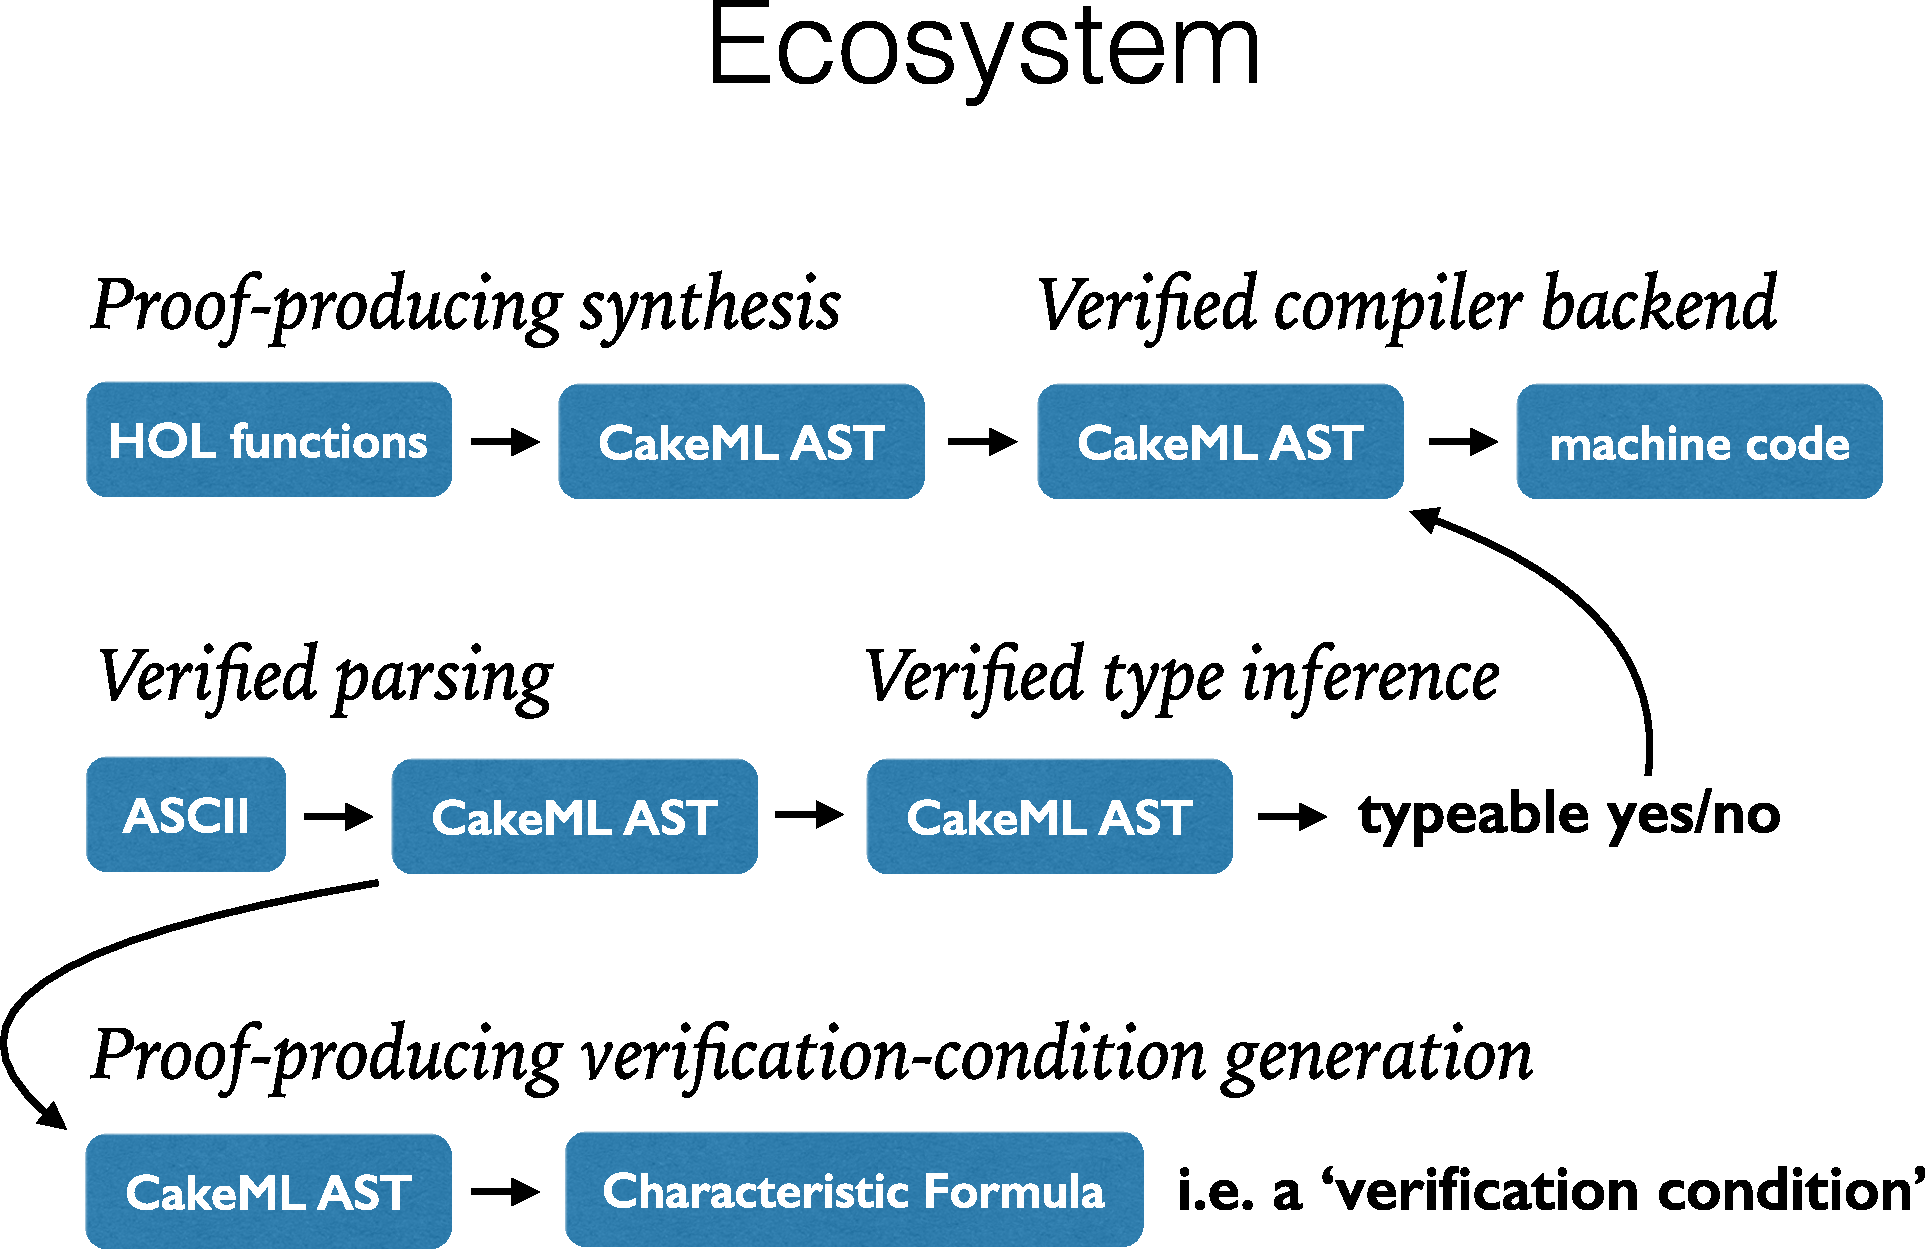
\includegraphics[width=\linewidth]{img/ecosystem.pdf}
  \caption[The CakeML ecosystem]{The CakeML ecosystem\footnotemark}
  \label{fig:intro:cakeml}
\end{figure}
\footnotetext{Image source: \url{https://cakeml.org/ecosystem.png}, used with permission}

\emph{CakeML} is a verified implementation of a subset of Standard ML \cite{kumar2014cakeml,tan2016cakeml}.
To quote the website, it is supplemented by ``an ecosystem of proofs and tools built around the language'' with the ``ecosystem [including] a proven-correct compiler that can bootstrap itself''.\footnote{\url{https://cakeml.org/}}
At time of writing, the project sports over forty developers and contributors.

\cref{fig:intro:cakeml} gives an overview over the ecosystem.
The verified part comprises a parser, type checker, formal semantics and backend for machine code.
The correctness proofs are carried out in the \emph{HOL4} system \cite{hol2014description}.
HOL4 is a proof assistant in the LCF family, similar to Isabelle.

CakeML is an integral part of this work.
My compiler produces CakeML abstract syntax trees and the correctness theorems are justified against its semantics.

\subsection{Semantics}

\begin{code}
  \centering
  \begin{subcode}{.4\linewidth}
    \begin{lstlisting}[language=ML]
type lit =
  | IntLit of integer
  | Char of char
  | StrLit of string
  | Word8 of word8
  | Word64 of word64\end{lstlisting}
  \end{subcode}
  \begin{subcode}{.4\linewidth}
    \begin{lstlisting}
datatype lit =
    IntLit int
  | Char char
  | StrLit string
  | Word8 (8 word)
  | Word64 (64 word)\end{lstlisting}
  \end{subcode}
  \caption{Lem specification of CakeML's type of literals and the resulting Isabelle text}
  \label{code:intro:cakeml:literals}
\end{code}

CakeML's semantics has been specified in \emph{Lem} \cite{mulligan2014lem}, ``a tool for lightweight executable mathematics''.\footnote{\url{https://www.cl.cam.ac.uk/~pes20/lem/}}
It provides a formal specification language that has features comparable to Isabelle/HOL; notably, definition of recursive types, functions and (inductive) predicates.
Lem is capable of compiling these specifications to other specification languages, including Isabelle, HOL4, and Coq.

The remainder of the CakeML ecosystem is implemented in HOL4.
For that, the developers maintain the CakeML semantics in Lem and compile it to HOL4.
Consequently, assuming trust in Lem, the version of the semantics that I use in Isabelle can be considered identical to the one in HOL4.
The Isabelle theories are available in the Archive of Formal Proofs~\cite{hupel2018cakeml}.

The CakeML formalization in Lem consists of multiple parts:
\begin{description}
  \item[Foundation libraries]
    Lem provides a standard library, notably for machine words.
  \item[Abstract syntax]
    As is usual in formalizations of programming languages, datatypes for expressions and values are provided.
  \item[Semantics]
    There are three flavours of semantics: (relational) big step, small step, and functional big step~\cite{owens2016functional}.
    For this thesis, only the big-step semantics is relevant.
\end{description}

\noindent
Note the absence of parsing and printing (i.e., concrete syntax).
This has been developed in HOL4 without the help of Lem, so a translation to Isabelle would be a significant undertaking.

\subsection{Compiler}

The simplest way for a user to interact with CakeML is to write some source code as they would for any other language.
The CakeML project provides a compiler that can be executed on x86-64 systems, producing a binary that may run on a variety of hardware platforms.
That compiler has itself been extracted from a formal specification.
Assuming the correctness of HOL4, every compilation guarantees that the resulting binary works correctly according to the semantics of the source program; in other words, compilation preserves semantics.

Another way to produce a binary program is to use the code extraction facility from HOL4 that goes directly to CakeML abstract syntax trees.
This thesis provides a similar tool, but implemented based on a different approach and for Isabelle/HOL specifications.
% !TeX spellcheck = en_GB
% !TeX encoding = UTF-8

\section{Motivation}
\label{sec:intro:motivation}

The purpose of using an interactive theorem prover -- or, more generally, any kind of prover -- is to provide high assurance and trust in the produced artifacts.
The range of applications is vast: program and hardware verification, automata and formal languages, security and confidentiality guarantees, analysis and probability theory, topology, and even general relativity, to name just a few~\cite{avigad2018milestones}.
The Isabelle community also runs a peer-reviewed repository of formal proof developments, the \emph{Archive of Formal Proofs}.\footnote{\url{https://www.isa-afp.org/}}

As outlined in §\ref{sec:intro:isabelle}, Isabelle is designed in such a way that proofs of statements that are accepted by the system can generally be considered to hold.
However, a proof is just a proof; in absence of other mechanisms, they ``do nothing''.
This is why the \emph{extraction} of (or equivalently, transformation into) executable code is not just an afterthought, but rather an important area of research.

While Isabelle offers a rich toolkit for functional programming and mathematical specifications, so far, there is no trustworthy translation to executable code.
This means that the guarantees provided by the system end at its boundaries.
The generated code bears -- apart from an unverified algorithm having produced it -- no connection to the original specification.
This thesis aims to bridge the gap by developing a verified compiler from Isabelle/HOL to CakeML.

The compiler operates in multiple stages that can be roughly characterized as \emph{preprocessing,} \emph{deep embedding,} and \emph{compilation phases}.
All stages are either \keyword{certifying} or \keyword{verified}, i.e., an error in the implementation of the compiler would lead to an Isabelle error that is displayed to the user.
Under no circumstances will the system emit executable code that once compiled produces an erroneous result.
% !TeX spellcheck = en_GB
% !TeX encoding = UTF-8

\section{Contributions}
\label{sec:intro:contrib}

Many theorem provers -- including Isabelle -- have the ability to generate executable code in some (typically functional) programming language from definitions, lemmas and
proofs~\cite{BerghoferN-TYPES00,Letouzey02,BoespflugDG11,Shankar01,PVS-attachments,GreveKMMRRSVW08,BoyerM02}.
This makes code generation part of the trusted kernel of the system.
Myreen and Owens~\cite{myreen2014translation} closed this gap for the HOL4 system: they have implemented a tool that translates specifications from HOL4 into \emph{CakeML}, a subset of SML, and proves a theorem stating that a result produced by the CakeML code is correct with respect to the HOL functions.
They also have a verified implementation of CakeML~\cite{kumar2014cakeml,tan2016cakeml}.

Here, I go one step further and provide a once-and-for-all verified compiler from (deeply embedded) function definitions in Isabelle/HOL~\cite{nipkow2014semantics} into CakeML proving partial correctness of the generated CakeML code with respect to the original functions.
This is comparable to the step from ``dynamic'' to ``static'' type checking.
It also means that preconditions on the input to the compiler are explicitly given in the correctness theorem rather than implicitly by a failing translation.

My compiler is in principle applicable to other languages than Isabelle/HOL or even HOL:
Types are erased right away.
Hence, the type system of the source language is irrelevant.
I merely assume that the source language has a semantics based on \emph{equational logic}.

All topics discussed in this thesis have been formalized in Isabelle; definitions and proofs are machine-checked.

\paragraph{Publications}
The following publications stem from work in this thesis:

\begin{itemize}[label=\faFileTextO]
  \item \fullcite{hupel2017lazycase}
  \item \fullcite{hupel2017constructor}
  \item \fullcite{hupel2017dict}
  \item \fullcite{hupel2018dict}
  \item \fullcite{hupel2018compiler}
  \item \fullcite{hupel2018cakeml}
  \item \fullcite{hupel2019algebra}
\end{itemize}
% !TeX spellcheck = en_GB
% !TeX encoding = UTF-8

\section{Structure of this thesis}

\begin{figure}[t]
  \tikzstyle{line} = [draw, dotted, thick]
  \tikzstyle{block} = [rectangle, fill=blue!20, text centered, text width=5em, minimum height=3em]
  \tikzstyle{gblock} = [block, fill=red!20]
  \tikzstyle{mblock} = [block, fill=green!20]
  \centering
  \begin{tikzpicture}
    \path [line] (0.5, 6) node [left] { ML } -- +(13.5, 0) ;

    \node [mblock] (pp) at (3.75, 6) { Pre\-processing };
    \node [above of=pp] { (§\ref{sec:preproc}) };

    \node [mblock] (embed) at (7.25, 6) { Deep embedding };
    \node [above of=embed] { (§\ref{sec:deep}) };

    \path [line] (0.5, 3) node [left] { HOL } -- +(13.5, 0) ;

    \node [block] (user) at (2, 3) { User definitions };

    \node [gblock] (simpl) at (5.5, 3) { Simplified definitions };

    \path [draw, thick] ([xshift=.2cm]user.north) |- ([yshift=.3cm]pp.south west);
    \path [draw, thick, -latex'] ([yshift=.3cm]pp.south east) -| ([xshift=-.2cm]simpl.north);

    \path [line] (0.5, 0) node [left] { \shortstack{Terms \\ (§\ref{sec:terms})} } -- +(13.5, 0) ;

    \node [gblock] (embedded) at (9, 0) { Embedded definitions };

    \path [draw, thick] ([xshift=.2cm]simpl.north) |- ([yshift=.3cm]embed.south west);
    \path [draw, thick, -latex'] ([yshift=.3cm]embed.south east) -| ([xshift=-.2cm]embedded.north);

    \node [gblock] (cake) at (12.5, 0) { CakeML program };

    \node [mblock] (compiler) at (10.75, 3) { Term compiler };
    \node [above of=compiler] { (§\ref{sec:compiler}) };

    \path [draw, thick] ([xshift=.2cm]embedded.north) |- ([yshift=.3cm]compiler.south west);
    \path [draw, thick, -latex'] ([yshift=.3cm]compiler.south east) -| ([xshift=-.2cm]cake.north);

    \node [block, fill=white] at (10.75, 6) { \phantom{Simplifier} }; % hack because checkerboard is transparent
    \node [mblock, pattern=checkerboard, pattern color=green!20, draw=green!20] (simp) at (10.75, 6) { Simplifier };

    \path [draw=black!50, thick, densely dotted] ([yshift=-.3cm]compiler.north west) -- ([yshift=-.3cm,xshift=-.25cm]compiler.north west) |- ([yshift=.3cm]simp.south west);
    \path [draw=black!50, thick, densely dotted, -latex'] ([yshift=.3cm]simp.south east) -- ([yshift=.3cm,xshift=.25cm]simp.south east) |- ([yshift=-.3cm]compiler.north east);
  \end{tikzpicture}

  \small
  \vspace{1em}
  \begin{tabular}{ll}
    % <https://tex.stackexchange.com/a/171785/172786>
    \cellcolor{green!20} & implemented as part of this thesis \\
    \multirow{-2}{*}{\cellcolor{green!20}green} & (checkered: already available in Isabelle) \\
    \cellcolor{blue!20}blue & specified by user \\
    \cellcolor{red!20}red & generated object
  \end{tabular}

  \caption{Stages of the compiler from Isabelle to CakeML}
  \label{fig:overview:structure}
\end{figure}

After this introduction, a chapter on technical preliminaries will follow (§\ref{sec:background}).
Subsequently, the thesis is roughly structured according to the phases of the compiler (\cref{fig:overview:structure}).
The diagram shows the source object as specified by the user and its transformation into the target object.
Each phase is driven by an implementation, which can either be a certifying one in ML, or a verified one in Isabelle/HOL (the difference is explained in more detail in §\ref{sec:background:terminology}).

The preprocessing phase statically eliminates features that are not supported by the compiler (§\ref{sec:preproc}).
Most importantly, the \keyword{dictionary construction} (§\ref{sec:preproc:dict}) eliminates uses of an advanced type system feature.

There are various term types that are required for later stages in the compiler.
§\ref{sec:terms} introduces a term algebra and discusses the differences between those types.

The \keyword{deep embedding} phase (§\ref{sec:deep}) lifts Isabelle terms into an internal model.
This allows reasoning about Isabelle terms in Isabelle itself.

There are multiple \emph{compiler phases} that process defining equations until a CakeML expression is reached.
These phases are described in §\ref{sec:compiler}.
% !TeX spellcheck = en_GB
% !TeX encoding = UTF-8

\section{How to read this thesis}

\authorship{
  A paragraph with a pencil indicates that the following section -- or portions thereof -- has appeared previously in another publication (§\ref{sec:intro:contrib}).
  Unless stated otherwise, in publications with a coauthor, I have contributed the majority of the content, including implementation.
}

\remark{
  Particularly thorny issues, or complicated design decisions stemming from restrictions of Isabelle or CakeML, are described in a box decorated with Bourbaki's dangerous bend symbol.
  They are not crucial for understanding and can be safely skipped.
}

\noindent
When describing a formalization, I frequently refer to theories.\thyrefafp{CakeML}{Ast}
Such references (for example to the Archive of Formal Proofs) appear in the margin.
For other non-bibliographic references, for example to external tools, I use footnotes.

Some sections in this thesis consist of large quantities of definitions, lemmas, and proofs.
They have been simplified and streamlined for better presentation.
Their actual Isabelle representation can be found in the formalization.

\setchapterpreamble{\dictum[Jean Chrétien]{A proof is a proof.\\
What kind of a proof?\\
It's a proof.\\
A proof is a proof,\\
and when you have a good proof,\\
it's because it's proven.}}

\chapter{Background}

\label{sec:background}
\vspace{1em}
% !TeX spellcheck = en_GB
% !TeX encoding = UTF-8

\noindent
This chapter describes in detail necessary technical background on Isabelle that is relevant for understanding the remainder of this thesis.

\section{Isabelle design}

One of the defining features of Isabelle as compared to other proof assistants in the same family is its modular logic design~\cite{paulson1990isabelle}:
the kernel provides the minimal logic \emph{Pure,} on top of which other logics can be implemented by users.
Pure, in its essence, is a framework for natural deduction proofs.
Proved statements are internally represented as values of the abstract type \mltype{thm}.
Standard ML's typing discipline ensures that such values can only be constructed through a finite set of primitives that represent rules or axiom schemas of constructive logic.

The most basic rule is \emph{modus ponens:} two statements $P \implies Q$ and $P$ can be combined to deduce $Q$.
As is common in literature, this thesis will frequently express such inferences using the following notation:
\[
  \inferrule*{P \implies Q \\ P}{Q}
\]

\noindent
Based on such primitives, a variety of automated \emph{tactics} are provided.
Tactics in their most basic form are ML programs that transform theorems into theorems.
This can be used for user interaction when proving theorems:
\begin{enumerate}
  \item
    The user indicates that they would like to prove the statement $P$.
  \item
    Because the system does not know yet that $P$ holds, it generates the \emph{goal state} $P \implies P$.
    A goal state is an implication whose premises are called \emph{subgoals} and the conclusion is the statement that the user wants proved.
    Observe that $P \implies P$ holds for all $P$: it is an axiom schema.
  \item
    The user can apply tactics that manipulate some (or all) subgoals.
    For example, a goal state $Q_1 \wedge Q_2 \implies P$ can be transformed into $Q_1 \implies Q_2 \implies P$; an instance of conjunction introduction, where a conjunction is split into two separate subgoals.
  \item
    Eventually, if all subgoals disappear (have been \emph{discharged}) and the goal state is $P$, the system will accept this as a proved statement.
    Because the goal state is a value of type \mltype{thm} at all times, $P$ is directly usable as a theorem.
\end{enumerate}

\noindent
Isabelle comes equipped with a set of standard tactics, for example the simplifier, which is able to rewrite terms according to (possibly conditional) rewrite rules $t \equiv u$, and a classical reasoner based on a tableau calculus~\cite{paulson1999generic}.

System interaction can happen on two ``layers'': the raw ML programming environment, or the high-level language Isar~\cite{wenzel2002isar}.
For most purposes, users do not manipulate low-level ML values, but can instead use the abstract Isabelle/Isar syntax.

\begin{code}[t]
  \begin{lstlisting}
datatype $\alpha$ seq = Empty | Seq $\alpha$ ($\alpha$ seq)

fun conc :: $\alpha$ seq $\Rightarrow$ $\alpha$ seq $\Rightarrow$ $\alpha$ seq where
conc Empty //ys// = //ys//
conc (Seq //x// //xs//) //ys// = Seq //x// (conc //xs// //ys//)\end{lstlisting}
  \caption{A simple functional program in Isabelle/HOL}
  \label{code:background:isabelle}
\end{code}

The most commonly used logic of Isabelle is \emph{Higher-Order Logic} (\emph{HOL} for short) based on work by Gordon~\cite{gordon1993hol}.
Besides standard features of classical higher-order logic (definitions, quantifiers, connectives) it provides tools for functional programming, e.g.\ recursive datatypes and functions with pattern matching.

\section{Terminology}
\label{sec:background:terminology}

The term \keyword{theory} has two meanings:
on a physical level, files containing Isabelle/Isar sources; on a theoretical level, a collection of definitions, constants, theorems, and other logical content.
A theory file is a sequence of Isar \emph{commands} that alter the logical theory.
I will frequently refer to the actual Isabelle source files that accompany this thesis as \emph{the formalization}.

Higher-level tools in Isabelle are usually referred to as \emph{packages}.
For example, the two facilities that enable functional programming are the \holcommand{function}\holcommandindex{function} and the \holcommand{datatype}\holcommandindex{datatype} packages~\cite{krauss2010recursive,krauss2009fun,blanchette2014datatypes}.
A simple example of their interplay is given in \cref{code:background:isabelle}.
Because in the architecture of Isabelle, all of these tools need to justify their constructions against the Isabelle kernel.
An implementation error would not produce an unsound theory; instead, the kernel would print an error that some construction failed.

Besides theorems, the second foundational ingredient of an Isabelle theory are \emph{constants}.
Contrary to what the name suggests, the type of a constant can also be a function type.
The logical distinction between constants and \emph{variables} in Isabelle is that constants may have definition (or multiple, see §\ref{sec:background:types}), whereas variables may not.
Datatype constructors and functions, as in \cref{code:background:isabelle}, are also constants, as far as the kernel is concerned; even though they have no user-accessible definition.
Still, they are internally constructed and defined by their respective packages.

Internally, Isabelle keeps track of a special kind of variable: \emph{schematic variables}\index{schematic variable}.
Schematic variables can be instantiated with arbitrary terms.
This is an implementation trick to avoid quantifiers in many situations.

A theory can be augmented with arbitrary auxiliary data.
A particular extension is referred to as a \emph{proof context,} or \emph{context} for short.
Contexts, for example, keep track of fixed variables and their types, and local assumptions that are not valid on the global theory level.
Most frequently, Isabelle users encounter contexts when they write a structured proof.
Furthermore, contexts enable modular reasoning (§\ref{sec:terms:prelim:modularity}).

\paragraph{Certifying and verified routines}
Consider a routine that takes a value $x$, transforms it according to a function $f$, and ensures that the result $y = f\;x$ satisfies a predicate $P$.
In proof assistants, there are two ways to implement this:
\begin{enumerate}
  \item
    A block of ML code analyses the value $x$, defines a new object $y$ and carries out a proof that $P\;y$.
    This proof may fail if the ML code has an error, or if some precondition is not satisfied.
  \item
    The function $f$ is implemented inside the logic, together with a proof that $P\;(f\;x)$ holds for all $x$.
    This is less flexible, but the routine has been shown to be correct once and for all.
\end{enumerate}

\noindent
The first strategy is known as \keyword{certifying}, because after each run, it produces a single certificate that the generated object is valid.
Contrary to that, the second one is called as \keyword{verified}, because the implementer has given a full correctness proof.
Both approaches have their own (dis)advantages, which means they are often mixed, such as in this formalization.

\paragraph{Notational conventions}
As can be observed in \cref{code:background:isabelle}, Isar notation is similar to that of programming languages like Haskell or ML.
For easier readability, code samples are slightly modified from their actual representation that can be processed by Isabelle.

By convention, types and constants are set in \holconst{typewriter} font.
Term variables are, as is usual in mathematics, set in $\mathit{italics}$.

An actual Isabelle source file (a \keyword{theory}) is composed of a sequence of commands.
Commands are set in \holcommand{sans-serif}.
Special syntactic constructs in terms, like branching, are written as $\holkeyword{if}\;P\;\holkeyword{then}\;x\;\holkeyword{else}\;y$.

\section{Type system}
\label{sec:background:types}

Isabelle implements an ML-style \emph{simple type system} with \emph{schematic polymorphism}.
Types can be formed by type constructors (e.g.\ \holtype{list}) and type variables ($\alpha, \beta, \ldots$).
Composite types are written in postfix notation, i.e., a list of integers is written as $\holtype{int}\;\holtype{list}$.
All types in HOL are non-empty, that is, they have at least one inhabitant.

\paragraph{Polymorphism}
Isabelle supports \emph{type schemes}\index{type scheme} (or \emph{polytypes} in recent literature) \cite{milner1978polymorphism,hindley1969principal}:
types can be quantified at the outermost level.
For example, $\forall \tau.\; \tau\;\holconst{list}$ is a valid type scheme for the empty list $[]$.
In contrast, $(\forall \tau.\; \tau\;\holconst{list})\;\holconst{list}$ is not admissible as a type scheme for the list containing the empty list $[[]]$, because the quantifier is nested inside a type constructor; i.e., no second-rank polymorphism is allowed~\cite{botlan2003mlf}.

To implement this, Pure does not provide an explicit type quantifier; instead, it uses schematic polymorphism.
In addition to type variables, there are also \emph{schematic type variables} that can be instantiated.\index{schematic variable}
Those are prefixed with a question mark: $?\alpha$.
This distinction becomes important later for technical reasons (§\ref{sec:preproc:dict:elim:impl}).
Users can largely ignore schematic type variables, as the system automatically introduces them.

\begin{code}
  \begin{lstlisting}
consts size :: $\alpha$ $\Rightarrow$ nat

overloading size_list $\equiv$ size :: $\alpha$ list $\Rightarrow$ nat
begin

  definition size_list where
  size_list = List.length

end
  \end{lstlisting}
  \caption{Declaration of a constant and overloaded definitions}
  \label{code:background:overloading}
\end{code}

\paragraph{Overloading}
Isabelle supports \emph{overloading} of constants based on their type.
It is possible to declare a constant with a polymorphic type and then give definitions for a specific instantiation~\cite{kuncar2018consistent}.
As an example, consider \cref{code:background:overloading} that declares a function that should represent the ``size'' of a value.
As defined there, it works for lists and can be extended for other types.

This mechanism is very flexible, but is hardly employed directly by users.
Instead, the system implements \emph{type classes} based on overloading.
Type classes are widely used in the Isabelle community and require special treatment for the purpose of this thesis (§\ref{sec:preproc:dict}).

\section{Executability}
\label{sec:background:code}

\index{executability|see{executable}}
Specifications formalized in Isabelle/HOL -- a classical logic -- are not necessarily \keyword{executable}.
This affects proofs who may use classical constructs like law of excluded middle and Hilbert choice.
However, this thesis is concerned with generating a functional program that can be compiled to machine code from Isabelle specifications.

This mismatch can be reconciled by identifying an executable subset of types and definitions that can be translated into a functional program.
Importantly, this is not a new concept and can be traced back to previous work in this area, most recently by Haftmann~\cite{haftmann2010codegeneration,haftmann2010haskell}.
In general, that subset can be characterized as ``functional program in, functional program out''.
However, there are a few notable exceptions:
HOL is more expressive than programming languages; for example, it is possible to quantify over an infinite set, which is naturally not executable.
By default, specifications that are created by \holcommand{datatype}\holcommandindex{datatype} and \holcommand{function}\holcommandindex{function} and that only use other executable functions are themselves executable:
these packages have been designed with executability in mind.

Apart from \holcommand{function}, which enables definition of recursive functions, there is also the \holcommand{definition}\holcommandindex{definition} command.
It only supports non-recursive, non-pattern-matching definitions.
For the purposes of this thesis, their internal implementation differences are not relevant: both allow introducing constants into a theory based on \emph{defining equations}\index{equation, defining}.

Isabelle's code generator also supports post-hoc introduction of executability of a specification.
Sometimes it can be more convenient to specify a constant using the non-executable fragment, for example using an unconstrained quantifier.
Later on, a \emph{code equation}\index{equation, code} can be added to the theory, which will then be used instead of the original defining equation (§\ref{sec:preproc:dict:current}).
Code equations can override any existing definition.
In a nutshell, a specification is executable if its transitive set of code equations only use recursion and pattern matching.
In this thesis, the term \emph{defining equation} is preferred, because the point at which they are introduced into the theory does not matter to the compiler.

Even though the term ``executability'' suggests some form of efficient program on hardware, it is not necessary that executable code has to be executed outside of Isabelle.
Most notably, the simplifier can be set up to only use the defining equations, which could be used to emulate a graph-reduction style~\cite{hudak1989conception} evaluation inside the Isabelle kernel.\thyrefdist{HOL-Real_Asymp}{Lazy_Eval}

When designing a specification, it is advantageous to stay within the executable fragment of HOL.
Many Isabelle tools aimed at developer productivity work better (or only work) in such cases.
The prime example is \holcommand{quickcheck}~\cite{bulwahn2012quickcheck}\holcommandindex{quickcheck}, which is able to uncover flaws in theorem statements by running an automated counterexample finder.
This saves a lot of time by preventing one from trying to prove false statements.
Consequently, in many parts of this thesis, I made design decisions supporting these tools (for example in §\ref{sec:background:cakeml}), even though at times it complicates the specifications.

\section{Inductive predicates}
\label{sec:background:inductive}

\begin{code}
  \begin{subcode}[b]{.49\linewidth}
    \[
      \inferrule*{ }{\holconst{even}\;0} \qquad
      \inferrule*{\holconst{even}\;n}{\holconst{even}\;(n + 2)}
    \]
    \caption{Mathematical characterization}
  \end{subcode}\hfill
  \begin{subcode}[b]{.49\linewidth}
    \begin{lstlisting}
inductive even :: nat $\Rightarrow$ bool where
even $0$ |
even //n// $\implies$ even (//n// + $2$)\end{lstlisting}
    \caption{Isabelle notation}
  \end{subcode}
  \vspace{1em}

  \begin{subcode}{\linewidth}
    \[
      \inferrule*{
        \holconst{even}\;x \\
        P\;0\\
        (\forall n.\; \holconst{even}\;n \implies P\;n \implies P\;(\holconst{Suc}\;n))
      }{P\;x}
    \]
    \caption{Induction principle}
  \end{subcode}

  \caption{A simple inductively defined predicate}
  \label{code:background:inductive}
\end{code}

Both in formal and informal mathematics, the notion of \emph{inductively defined,} or \emph{inductive predicates}\index{predicate, inductive} is pervasive.
Winskel~\cite{winskel1993semantics} gives a comprehensive introduction into their mathematical background.
Parts of this will be revisited in later chapters, notably well-founded induction.

\cref{code:background:inductive} presents a simple inductive characterization of even numbers.
The two rules declare that $0$ is even, and if $n$ is even, so is $n+2$.
The result of this abstract specification is the smallest predicate $\holtypejudgement{\holconst{even}}{\holtype{nat}\Rightarrow\holconst{bool}}$ satisfying the given rules, i.e., the \emph{least fixed point}.
Literature commonly uses inductive sets instead of predicates; however, the types $\alpha\;\holconst{set}$ and $\alpha\Rightarrow\holconst{bool}$ are isomorphic to each other.

\remark*{
  In Isabelle post-2012 versions, sets and predicates are distinct types and many libraries are duplicated for both.
  In this formalization, predicates are preferred, unless finitary constraints need to be enforced.
}

\noindent
In Isabelle, the \holcommand{inductive}\holcommandindex{inductive} package can be used to introduce inductive predicates.
The \holcommand{inductive} command automates the internal construction of a least fixed-point based on the given rules, which are referred to as \emph{introduction rules}\index{introduction rule}.
Conversely, there are also \emph{elimination rules}\index{elimination rule}.
They can be used to prove properties like $\holconst{even}\;(n + 2) \implies \holconst{even}\;n$.

The command also generates an induction schema.
In the \holconst{even} example, it can be used to prove properties of the form $\holconst{even}\;n \implies P\;n$ for arbitrary $P$.
This is usually referred to as \keyword{rule induction}.

Inductively defined predicates are the most important ingredient for defining semantics.
Nipkow and Klein~\cite[§4.5]{nipkow2014semantics} give further explanations of how those work in Isabelle.
In fact, the example in \cref{code:background:inductive} is taken from their book.

Semantics for non-trivial languages, including CakeML, are not purely specified as inductive predicates.
Frequently, they are based on \emph{semantic functions}\index{semantic function} which are used to carry out substitution, matching, and other fundamental operations.

Inductive predicates are convenient to use because contrary to function definitions, users need not care about termination.
For example, one can define a big-step semantics for a programming language that admits non-terminating programs.
It is not possible to define this in an equational way without additional tricks~\cite{owens2016functional,spector2018haskell}.

\remark*{
  There are still constraints on the kinds of rules that can constitute a least-fixed point, but these can often be automatically discharged by the \holcommand{inductive} package.
  When higher-order predicates are involved (for example $\holtypejudgement{\holconst{pred}_{\holtype{list}}}{(\alpha \Rightarrow \holtype{bool}) \Rightarrow \alpha\;\holtype{list} \Rightarrow \holtype{bool}}$), monotonicity has to be proved by the user first.
}

\noindent
The obvious downside resulting from that convenience is that inductive predicates are by default not executable (§\ref{sec:background:code}).
Berghofer \etal~\cite{berghofer2009inductive} have introduced a \emph{predicate compiler} which can transform a large fragment of inductive specifications into executable code.
While it works mostly automatically, it is tricky to use and has several edge cases; as such, I consider it to be a feature of last resort and prefer equational definitions where possible.

\remark*{
  In the \holconst{even} example, the predicate compiler produces code equations that terminate for even numbers -- correctly answering \holconst{True} -- but fail to terminate for odd numbers.
  The reason is that the compiler does not know that the search for an $n'$ such that $n = n' + 2$ is bounded.
}

\noindent
The categorical dual, \emph{coinductive} predicates\index{predicate, coinductive}, are only needed at single point in the formalization (\cref{code:intermediate:ml:corr}).
Because of their only brief appearance, an explanation of coinduction is out of the scope for this thesis.
I refer the reader to the literature for more details \cite{sangiorgi2011coinduction,gordon1995coinduction}.

\section{Term rewriting}
\label{sec:background:rewriting}

\begin{code}
  \begin{subcode}{.3\linewidth}
    \begin{lstlisting}[language=Isabelle]
datatype term =
  Const string |
  Free string |
  Abs term |
  Bound nat |
  App term term
    \end{lstlisting}
    \caption{Abstract syntax of de~Bruijn terms}
    \label{code:background:rewriting:term}
  \end{subcode}
  \begin{subcode}{.7\linewidth}
    \[
      \inferrule*[left=Step]{(\mathit{lhs}, \mathit{rhs}) \in \R \\ \holconst{match}\;\mathit{lhs}\;t = \holconst{Some}\;\sigma}{\rewrite{\R}{t}{\holconst{subst}\;\sigma\;\mathit{rhs}}}
    \]
    \[
      \inferrule*[left=Beta]{ }{\rewrite{\R}{\app{(\Lambda t)}{t'}}{t[t']}} \quad
      \inferrule*[left=Fun]{\rewrite{\R}{t}{t'}}{\rewrite{\R}{\app t u}{\app{t'}{u}}}
    \]
    \[
      \inferrule*[left=Arg]{\rewrite{\R}{u}{u'}}{\rewrite{\R}{\app t u}{\app{t}{u'}}}
    \]
    \caption{Small-step semantics}
    \label{code:background:rewriting:semantics}
  \end{subcode}
  \caption{Overview of the deeply embedded de Bruijn \holtype{term} type}
\end{code}

\noindent
Based on the internal definition of terms in Isabelle/Pure, one can model terms as a datatype in HOL: the \emph{deeply embedded term language} is depicted in~\cref{code:background:rewriting:term}.
Similarly to the Pure type, it uses \emph{de~Bruijn indices}~\cite{debruijn1972lambda}\index{de Bruijn index}, but omits types and schematic variables.

The embedded HOL \holtype{term}\holtypeindex{term} type uses the same conventions as its ML counterpart.\holmlindex{term}
I write $\holconst{App}\;t\;u$\holconstindex{App} as $\app t u$\index{\$@\$ (symbol)} and $\holconst{Abs}\;t$\holconstindex{Abs} as $\Lambda\;t$\index{$\Lambda$@$\Lambda$ (symbol)}.
The notation $t [t']$ represents $\beta$-reduction\index{beta-reduction@$\beta$-reduction}, that is, substitution of the innermost bound variable (i.e.\ with index zero) in $t$ with $t'$ (the implementation of $\beta$-reduction will be revisited in §\ref{sec:terms:types:term}).
Throughout this thesis, I will use an upper-case $\Lambda$ to refer to the concrete syntax of abstraction in the embedded term language, whereas lower-case $\lambda$ is used for Pure abstractions.
More details on this and other term types can be found in §\ref{sec:terms}.

Observe that types are not preserved in this embedded language.
In Pure, the \holconst{Const}\holmlindex{Const}, \holconst{Free}\holmlindex{Free}, and \holconst{Abs}\holmlindex{Free} constructors carry type information, each for a different purpose:
constants can be polymorphic (the type specifies the instantiation of the type scheme), free variables are identified by their name and their type (there may be multiple variables with the same name but different types), and finally, abstractions specify the type of the bound variable.

\remark*{
  While type checking admits multiple variables with the same name and differing types, it rarely happens in practice because type inference rejects such terms.
  If a user was to feed, for example, the term $x\cons x$ into Isabelle (where $\cons$ is list cons)\index{\#@$\cons$ (symbol)}, type inference would report a unification failure, because $\alpha$ and $\alpha\;\holtype{list}$ cannot be unified.
  Consequently, it is no real restriction that the model presented here does not handle such odd terms.
}

\noindent
For abstractions, type erasure is unproblematic, because they are assumed to be parametric; i.e., for a polymorphic parameter, they may not behave differently depending on the concrete instantiation.
However, it becomes impossible to distinguish between different instantiations of constants.
This is problematic because of overloading (§\ref{sec:background:types}).
I employ the so-called dictionary construction (§\ref{sec:preproc:dict}) to avoid this problem.

\cref{code:background:rewriting:semantics} specifies the small-step semantics for terms.
It is reminiscent of \emph{higher-order term rewriting}, and modelled closely after equality in HOL.
The basic idea is that if the proposition $t = u$ can be proved equationally in HOL (without symmetry), then $\rewrite*\R{\embed t}{\embed u}$ holds, where \R\ contains all defining equations.
The angle brackets denote the deep-embedding operator that will be explained in more detail in §\ref{sec:deep}.

In the semantic for terms with de Bruijn indices, substitution under binders, i.e., rewriting below an abstraction, can be easily implemented: there are no bound variable names that could capture free variables of the term that is substituted.
Still, the semantics in \cref{code:background:rewriting:semantics} does not recurse below binders; only below application.
The reason for that is twofold:
\begin{enumerate}
  \item during the process of the compiler, new term types are introduced that carry explicit bound variable names (§\ref{sec:terms:types}), and
  \item in the CakeML semantics, substitution does not happen below binders (§\ref{sec:intermediate:cakeml}).
\end{enumerate}

\noindent
This model of term rewriting in HOL coincides by design with the notion of executability.
All defining equations can be lifted into the set \R, which will then be transformed in later stages of the compiler.

\section{CakeML/Isabelle integration}
\label{sec:background:cakeml}

Because the Lem specification of CakeML assumes some special features of HOL4, some adaptations were necessary:
\begin{itemize}
  \item
    Fabian Immler and Johannes Åman Pohjola have contributed to the adaptation of machine words and floating-point arithmetic.
  \item
    Pohjola has contributed the s-expression printer that converts CakeML programs into string form, which can subsequently be consumed by the CakeML compiler.
  \item
    The functional big step semantics is implemented using a special function to enforce monotonically decreasing clocks according to Kumar and Myreen \cite[§3.2]{kumar2018clocked}.\thyrefafp{CakeML}{Evaluate_Clock}
    This makes the termination proof simpler, but complicates reasoning about the semantics.\thyrefafp{CakeML}{Big_Step_Fun_Equiv}
    Proofs from HOL4 that rephrase the semantics without that function had to be ported to Isabelle.
    Additionally, the equivalence proofs between big step and functional big step semantics were ported.
  \item
    In general, Isabelle tools and automation work better with nested recursive definitions instead of mutually recursive definitions.\thyrefafp{CakeML}{Evaluate_Single}
    Additionally, my formalization ignores certain features of CakeML; notably mutable cells, modules, and literals.
    Consequently, I have derived a smaller, executable version of the original CakeML semantics, together with an equivalence proof, called \emph{CupCakeML} (§\ref{sec:intermediate:cakeml}).\thyrefmy{CupCake_Semantics}
    Portions of this have been implemented by Yu Zhang.
  \item
    Where necessary, I have set up code equations and \holcommand{quickcheck} for more rapid development of theories.\thyrefafp{CakeML}{CakeML_Quickcheck}
    In general, the functional big step semantics is better suited for executability than the relational variant, because it is defined as a \holcommand{function}.
\end{itemize}

\noindent In order to obtain a full toolchain from Isabelle definitions to machine code, I have implemented a small pretty-printer of the CupCakeML fragment to concrete CakeML syntax, which is part of the trusted code base.\thyrefafp{CakeML}{CakeML_Compiler}
The resulting source text can then be fed into the CakeML compiler.


\setchapterpreamble{\dictum[Old Isabelle proverb]{
  Axiomatic type classes are definitional.\\
  Type definitions are axiomatic.
}}

\chapter{Preprocessing definitions}
\minitoc

\label{sec:preproc}
% !TeX spellcheck = en_GB
% !TeX encoding = UTF-8

\noindent
Before definitions can be processed by the compiler, a \emph{preprocessing} phase needs to modify them to remove unsupported features.
This chapter explains these steps, starting with the elimination of type classes (§\ref{sec:preproc:dict}), followed by lazy evaluation of case combinators (§\ref{sec:preproc:lazy}) and partially applied constructors (§\ref{sec:preproc:constructor}).
Finally, it deals with restrictions on pattern matching (§\ref{sec:preproc:compatibility}) and other limitations (§\ref{sec:preproc:limitations}).
% !TeX spellcheck = en_GB
% !TeX encoding = UTF-8

\section{Dictionary construction}
\label{sec:preproc:dict}
\index{dictionary construction}

\authorship{
  Portions of this section appear in the AFP entry \citetitle{hupel2017dict} (\citeauthor{hupel2017dict}~\cite{hupel2017dict}), and the preprint \citetitle{hupel2018dict} (\citeauthor{hupel2018dict}~\cite{hupel2018dict}).
  Users are recommended to refer to that AFP entry for latest documentation.
}

\noindent
Isabelle/Pure features \emph{type classes}~\cite{haftmann2007typeclasses,wenzel1997typeclasses}.
These are built into the kernel and are used extensively in theory developments.
The code generator, when targeting Standard ML, performs the well-known dictionary construction or \emph{dictionary translation}~\cite{haftmann2010codegeneration}.
This works by replacing type classes with records, instances with values, and occurrences with explicit parameters.

Similarly to Standard ML, CakeML does not support type classes.
To avoid complicating the correctness proofs, I decided to also not support them in the embedded term language (§\ref{sec:background:rewriting}).
Instead, a \emph{dictionary construction} eliminates classes and instances before embedding into the term language.
This section deals with the chosen encoding of type classes and instances, the certifying translation, and treatment of partial functions.

\subsection{Preliminaries}
\label{sec:preproc:dict:prelim}

\index{class parameter|see{class constant}}
\index{type class|see{class}}

In Isabelle parlance, the term \keyword{class} refers to a type class; a concept known from Haskell~\cite{wadler1989adhoc,haftmann2007typeclasses}.
A class can fix a type $\alpha$ and some constants whose type contains $\alpha$.
Those constants are officially referred to as \emph{class parameters}.
Classes and parameters live in different name spaces.
In the example in \cref{code:preproc:dict}, \holconst{plus} is a parameter of the \holconst{plus} class.
In this section, I will use the term \keyword{class constant} instead of class parameter, to avoid the ambiguity with function parameters.

A set of classes is called a \keyword{sort}.
Type variables may carry \emph{sort constraints}\index{sort constraint}, which are preceded by double colons: $\holtypejudgement{\alpha}{\{ \holclass{plus}, \holclass{times} \}}$.
Formally, a sort is an intersection of classes: the set of types that satisfy the sort $\{ \holclass{plus}, \holclass{times} \}$ is the set of the types have both a \holclass{plus} and a \holclass{times} \keyword{instance}.
Constants are said to have sort constrains if their types contain type variables with sort constraints.
Sort constraints can be omitted by the user and will be inferred.
If they are provided by the user, it is sufficient to specify them once per type variable.

As an example, consider the function $\holconst f\;x = x + x$.
In HOL, the $+$ operator is defined in the type class \holclass{plus}.
This means that the type of \holconst{f} is $(\holtypejudgement{\alpha}{\holclass{plus}}) \Rightarrow \alpha$.

Classes can extend other classes, with the inheritance relationship forming a directed acyclic graph (and with it, a partial order).
Sorts can be normalized according to this partial order.
Assuming that the class \holclass{group} extends both \holclass{zero} and \holclass{plus}, the sort $\{ \holclass{group}, \holclass{zero} \}$ can equivalently be written as $\{ \holclass{group} \}$.
I always assume that sorts are \emph{normal.}

Largely, classes work similarly in Haskell -- Haskell98, to be specific -- and Isabelle (see also §\ref{sec:preproc:dict:related}).
Isabelle's type system does not admit type constructor classes, nor other extensions like multi-parameter classes or undecidable instances.
However, Isabelle offers major enhancements over Haskell:
\begin{itemize}
  \item
    Isabelle being a proof assistant allows \emph{class axioms}\index{class axiom} that must be proved for every type that wishes to instantiate the class.
    The precise axioms are irrelevant for the dictionary construction (§\ref{sec:preproc:dict:elim:encoding}); they are abstracted as a predicate.
  \item
    It is possible to add edges in the inheritance relationship after the definition of the classes, as long as the user is able to produce a proof that the subclass axioms imply the superclass axioms.
\end{itemize}

\remark*{
  While parts of the dictionary construction are implemented incrementally, modifications in the class graph after their records have already been generated are not supported.
}

\subsection{Elimination of classes}
\label{sec:preproc:dict:elim}
The basic idea is to replace classes by \emph{dictionaries}\index{dictionary} containing all class constants and to replace instances by values.
Constants with sort constraints are rewritten in a way that they require additional dictionary parameters.

This transformation is an integral part of Isabelle's code generator.
It is described in detail by Haftmann and Nipkow \cite[§4]{haftmann2010codegeneration}, together with an informal correctness proof.

\begin{code}
  \begin{subfigure}{\linewidth}
    \begin{lstlisting}[language=Isabelle]
class plus =
  fixes plus :: $\alpha$ $\Rightarrow$ $\alpha$ $\Rightarrow$ $\alpha$ (infixl + 65)

definition f :: $\alpha$::plus $\Rightarrow$ $\alpha$ where
f //x// = //x// + //x//
    \end{lstlisting}
    \vskip-1.5em
    \caption{Source program}
  \end{subfigure}

  \vspace*{1em}
  \begin{subfigure}{\linewidth}
    \begin{lstlisting}[language=ML]
type 'a plus = {plus : 'a -> 'a -> 'a};
val plus = #plus : 'a plus -> 'a -> 'a -> 'a;

fun f dict x = plus dict x x;
    \end{lstlisting}
    \vskip-1.5em
    \caption{Target program (Standard ML)}
  \end{subfigure}
  \caption{Dictionary construction in Isabelle (current state)}
  \label{code:preproc:dict}
\end{code}

A complete example for $\holconst f\;x = x + x$ is reproduced in \cref{code:preproc:dict}.
Note that this translation is only required for target languages that do not support type classes (OCaml, Standard ML).
For other languages (Haskell, Scala), type classes are preserved with only minor syntactic changes.

\subsubsection{Current state}
\label{sec:preproc:dict:current}

In the code generator, the dictionary construction happens outside the logic.
It starts with a set of defining equations that represent the program to be exported.
These equations are proper theorems and are generated automatically by various commands for datatype and function definitions.
To improve efficiency, the user may provide alternative (verified) equations, for example, to replace a naive recursive implementation of a function by a more stack-efficient tail-recursive definition.

Then, these equations are internalized into an intermediate language.
The dictionary construction then proceeds in this internal language, following the approach outlined by Hall \etal~\cite{hall1996classes}.

\subsubsection{Certifying translation}
\label{sec:preproc:dict:elim:cert}

In this work, dictionary translation is performed before internalizing the defining equations into the deeply embedded term language.
It is a procedure implemented in ML which takes existing HOL definitions and produces new, derived HOL definitions, coupled with theorems certifying their equivalence.

\begin{code}
  \begin{lstlisting}[language=Isabelle]
datatype $\alpha$ dict_plus = mk_plus (const_plus: $\alpha$ $\Rightarrow$ $\alpha$ $\Rightarrow$ $\alpha$)

definition cert_plus :: $\alpha$::plus dict_plus $\Rightarrow$ bool where
cert_plus //dict// = (const_plus //dict// = plus)

fun f' :: $\alpha$ dict_plus $\Rightarrow$ $\alpha$ $\Rightarrow$ $\alpha$ where
f' //dict// //x// = const_plus //dict// //x// //x//

lemma f'_eq: cert_plus //dict// $\implies$ f' //dict// = f
(* proof omitted *)
  \end{lstlisting}
  \caption{Source program after dictionary construction in HOL (certifying translation)}
  \label{code:preproc:dict:hol}
\end{code}

To continue with the above example:
My mechanism introduces a derived constant \holconst{f'} with an additional dictionary parameter $\holtypejudgement{\mathit{dict}}{\alpha\;\holtype{dict\_plus}}$.
Then, it proves a theorem stating that for any \emph{valid} dictionary $\mathit{dict}$, \holconst{f'} is equivalent to \holconst{f}:
\[ \holconst{cert\_plus}\;\mathit{dict} \implies \holconst{f'}\;\mathit{dict} = \holconst{f} \]
Validity of a dictionary is captured by the $\holconst{cert\_plus}$ predicate.
Intuitively, $\holconst{cert\_}c\;\mathit{dict}$ means that $\mathit{dict}$ represents a known and lawful instance of class $c$.
The precise notion of ``validity'' is mainly dictated by technical considerations and discussed in the following section.

Additionally, for each type class instance $\holtypejudgement{\kappa}{(s_1, \ldots, s_k)\;c}$, where $\kappa$ is an $k$-ary type constructor and $s_i = \{c_{i,1}, \ldots, c_{i,n_i}\}$ are sorts, a new constant $\holconst{inst\_}c\holconst{\_}\kappa$ is defined.
Given the dictionaries for the $s_i$, it computes the dictionary for $\holtypejudgement{\kappa}{c}$.
Its correctness theorem is of the form
\[
  \left(\bigwedge\limits_{i=1}^{k} \bigwedge\limits_{j=1}^{n_i} \holconst{cert\_}c_{i,j}\;\mathit{dict}_{1,1}\right) \implies \holconst{cert\_}c\;(\holconst{inst\_}c\holconst{\_}\kappa\;\mathit{dict}_{1,1}\;\ldots\;\mathit{dict}_{1,n_1}\;\ldots\;\mathit{dict}_{k,1}\;\ldots\;\mathit{dict}_{k,n_k})
\]

\noindent For both instances and constants, each constituent class of each type variable's sort constraints gets assigned a dictionary argument and a premise certifying its validity.

The resulting program (as it would have been written by a user) is reproduced in \cref{code:preproc:dict:hol}.
My procedure defines the types and constants through the ML interfaces of various Isabelle packages, that is, users never see its results directly.
Instead, users would write \lstinline~declassify f~, which is a command that has the same effect as the hand-written definitions in \cref{code:preproc:dict:hol}.

\subsubsection{Possible encodings}
\label{sec:preproc:dict:elim:encoding}

The choice of the representation of dictionaries is straightforward:
I can model it as a datatype, along with functions returning values of that type.
The alternative here would have been to use Isabelle's extensible records \cite{naraschewski1998record}.
The obvious advantage of records is that I could easily model subclass relationships through record inheritance.
However, records do not support multiple inheritance.
Consequently, records offer no advantage over datatypes.
Instead, I opted for the more modern \holcommand{datatype} command \cite{blanchette2014datatypes}.
As of Isabelle2018, I have also introduced a \holcommand{datatype\_record} command that provides a subset of the syntax of records, but internally constructs a datatype.%
\thyrefdist{HOL-Library}{Datatype_Records}

A more controversial design question is how to represent dictionary certificates.
For example, given a value of type $\holtype{nat}\;\holtype{dict\_plus}$, how can one know that this is a faithful representation of the \holclass{plus} instance for \holtype{nat}?

\begin{enumerate}
  \item
    Florian Haftmann, in private communication, proposed a shallow encoding.
    It works by exploiting the internal treatment of constants with sort constraints in the Isabelle kernel.
    Constants themselves do not carry sort constraints, only their defining equations.
    The fact that a constant only appears with these constraints on the surface of the system is a feature of type inference.

    Instead, I can instruct the system to ignore these constraints.
    Isabelle's logic supports definitions of \emph{subtypes:}
    a type copy of an existing type that imposes additional constraints on values.
    For example, non-empty lists can be defined as a copy of lists with the constraint $\mathit{xs} \neq []$.
    Because HOL is a total logic, i.e., all types are non-empty, the system demands a witness satisfying the constraint.

    Applied to this situation, the key idea is to introduce a new type with a parameter $\alpha$ and the constraint that $\alpha$ implements a type class.
    However, this is ultimately futile:
    The nonemptiness proof requires a witness of a valid dictionary for an arbitrary, but fixed type $\alpha$, which is of course not possible, because type classes in general cannot be instantiated for all types.%
    \thyrefafp{Dict_Construction}{Impossibility}
  \item
    The certificates contain the class axioms directly.
    For example, the \holclass{semigroup\_add} class requires $(a + b) + c = a + (b + c)$.
    Such certificates are already defined for each class by Isabelle.
    Transferred to this setting, they would like this:
    %
    \begin{lstlisting}[language=Isabelle]
definition cert_plus :: $\alpha$ dict_plus $\Rightarrow$ bool where
cert_plus //dict// = ($\forall$//x// //y// //z//. const_plus //dict// (const_plus //dict// //x// //y//) //z// =
                               const_plus //dict// //x// (const_plus //dict// //y// //z//))\end{lstlisting}
    %
    Proving that instances satisfy this certificate is trivial.
    However, the equality proof of a constant before and after the construction is impossible: they are simply not equal in general.
    Nothing would prevent someone from defining an alternative dictionary using multiplication instead of addition and the certificate would still hold; but obviously functions using \holconst{plus} on numbers would expect addition.
    Intuitively, this makes sense: the above notion of certificate establishes no connection between original instantiation and newly generated dictionaries.

    Instead of proving equality, one would need to lift all existing theorems over the old constants to the new constants.
    This requires proof terms and replaying all proofs accordingly, which would be prohibitively expensive.
  \item
    In order for equality between new and old constants to hold, the certificate needs to capture that the dictionary corresponds exactly to the class constants.
    This is achieved by the representation in \cref{code:preproc:dict:hol}.
    It literally states that the fields of the dictionary are equal to the class constants.
    The condition of the resulting equation can only be instantiated with dictionaries corresponding to existing class instances.
    This constitutes a \emph{closed world} assumption, i.e., callers of generated code may not invent own instantiations.
\end{enumerate}

\noindent
My choice of representation is the third of these possibilities:
I expect dictionaries to be identical to the class constants.
For the user, that means that the conditions of the equivalence theorems ($\holconst{f'}\;\mathit{dict} = \holconst{f}$) can only be instantiated with existing class instantiations.
Unconditional equivalences can be achieved by monomorphizing constants.
Applied to the example in \cref{code:preproc:dict}, that would mean defining a constant $\holtypejudgement{\holconst{f}_\holtype{nat}}{\holtype{nat} \Rightarrow \holtype{nat}}$.
Its correctness theorem is unconditional, because no sort constraints occur in the type of \holconst{f}.

\subsection{Implementation}
\label{sec:preproc:dict:elim:impl}

The mechanism that transforms defining equations is similar to the one described by Haftmann and Nipkow~\cite[\S 4]{haftmann2010codegeneration}, which is presently used by the code generator to target OCaml and Standard ML.

\begin{figure}[t]
  \begin{subfigure}{.49\linewidth}
    \begin{lstlisting}[language=Isabelle]
class plus =
  fixes plus :: $\alpha$ $\Rightarrow$ $\alpha$ $\Rightarrow$ $\alpha$

instantiation nat :: plus
begin

fun plus_nat where
$0$ + //n// = (//n//::nat)
Suc //m// + //n// = Suc (//m// + //n//)

instance ..

end

definition f :: $\alpha$::plus $\Rightarrow$ $\alpha$ where
f //x// = //x// + //x//

(* f specialized to nat *)
definition g :: nat $\Rightarrow$ nat where
g //x// = f //x//
    \end{lstlisting}
  \end{subfigure}
  \begin{subfigure}{.49\linewidth}
    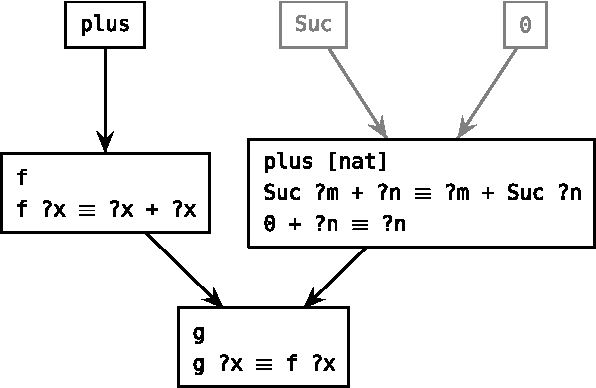
\includegraphics[width=\linewidth]{img/code-deps.pdf}
  \end{subfigure}
  \caption[A slightly extended source program and its code graph]{A slightly extended (from \cref{code:preproc:dict}) source program and its code graph}
  \label{fig:preproc:graph}
\end{figure}

Translating constants is the top-level operation in the dictionary construction.
The user invokes it with a set of constants.
Internally, the procedure uses existing mechanisms in Isabelle to obtain the \emph{code graph} of that set.
That graph contains all defining equations of the set and of all its transitive dependencies (i.e., other constants).
Each of these dependencies has to be re-defined as a new constant in some way, depending on whether or not it is a class constant.

\remark*{
  Strictly speaking, data constructors are also constants that may have class constraints.
  The dictionary construction does not support those in general.
  Additionally, the underlying type definition based on bounded natural functors largely ignores sort constraints.\footnote{\url{https://lists.cam.ac.uk/pipermail/cl-isabelle-users/2018-May/msg00065.html}}
  Consequently, they do not participate in the dictionary construction and are not relevant for this section.
}

\noindent
Along the way, auxiliary objects must be defined, for example the dictionary types for classes.
Unlike with the existing code generator, all of these steps need to be carried out inside the logic and are hence bound by its constraints.
Most notably, all definitions must be sequentialized to avoid forward references.
This means the implementation comprises mutually recursive, state-updating functions.

The code graph of a small program is given in \cref{fig:preproc:graph}.
As can be seen, the constant \holconst{g} depends on the constant \holconst{f} and the instance \holtypejudgement{\holtype{nat}}{\holclass{plus}}.
The data constructors \holconst{Suc} and \holconst{0} are greyed out.
The graph has to be traversed in topological order.

\remark*{
  Readers familiar with Isabelle's internals will notice that the code graph has been slightly redacted: The zero constructor for \holtype{nat} is actually the overloaded constant \holconst{zero} from the type class \holconst{zero}.
  This introduces technical complications, but does not in principle affect the dictionary construction.
}

\noindent
Throughout this section, the overloaded notations $\dict{\cdot}$ and $\dictinst{\cdot}$ are used to describe the translation of various kinds of objects.
I will first explain how types and classes themselves are processed.
Then, assuming a translation for terms exists, I will give a translation for type schemes and constants.
Lastly, the knot is tied by explaining how terms are processed.
In the actual implementation, all of these steps are intertwined.

\subsubsection{Types}

Recall that Isabelle distinguishes between type variables and schematic type variables\index{schematic variable} (§\ref{sec:background:types}).
Simple types, i.e., types that contain no schematic type variables, can be translated very easily: $\dict{\tau}$ forgets all sort constraints.
This is possible because those cannot have intrinsic sort constraints; those are imposed from the context and will be introduced accordingly when dealing with type schemes, which will be explained later.

\begin{code}[t]
  \begin{lstlisting}
datatype $\alpha$ dict_//c// = mk_//c//
  (super_$c_1$: $\alpha$ dict_$c_1$) (super_$c_2$: $\alpha$ dict_$c_2$) $\ldots$ (super_$c_n$: $\alpha$ dict_$c_n$)
  (const_$f_1$: $\dict{\tau_1}$) (const_$f_2$: $\dict{\tau_2}$) $\ldots$ (const_$f_m$: $\dict{\tau_m}$)

definition cert_//c// :: $\alpha$:://c// dict_//c// $\Rightarrow$ bool where
cert_//c// //dict// =
  (cert_$c_1$ (super_$c_1$ //dict//) $\wedge$ cert_$c_2$ (super_$c_2$ //dict//) $\wedge$ $\ldots$ cert_$c_n$ (super_$c_n$ //dict//) $\wedge$
   const_$f_1$ //dict// = $f_1$ $\wedge$ const_$f_2$ //dict// = $f_2$ $\wedge$ $\ldots$ $\wedge$ const_$f_m$ //dict// = $f_m$)
  \end{lstlisting}
  \caption{Dictionary datatype and certificate predicate}
  \label{code:datatype-cert}
\end{code}

\subsubsection{Classes}

A class $c$ over a type variable $\alpha$ may have superclasses $c_1, c_2, \ldots, c_n$ and constants $\holtypejudgement{f_1}{\tau_1}, \ldots, \holtypejudgement{f_m}{\tau_m}$.
Assuming the set $\{ c_1, c_2, \ldots, c_n\}$ is normal, this generates the definitions in \cref{code:datatype-cert}.
Note that the only type variable that may occur in the $\tau_i$ is $\alpha$ itself, which is an Isabelle restriction.
Consequently, it is not necessary to perform a recursive dictionary translation on the class constants, and I can get away with using the translation for simple types.

This newly introduced constructor and its fields have the following types:
\begin{align*}
  \holconst{mk\_}c &\holdoublecolon \alpha\;\holconst{dict\_}c_1 \Rightarrow \ldots \Rightarrow \alpha\;\holconst{dict\_}c_n \Rightarrow \alpha\;\holconst{dict\_}c \\
  \holconst{const\_}f_i &\holdoublecolon \alpha\;\holconst{dict\_}c \Rightarrow \dict{\tau_i} \\
  \holconst{super\_}c_i &\holdoublecolon \alpha\;\holconst{dict\_}c \Rightarrow \alpha\;\holconst{dict\_}c_i \\
  \holconst{cert\_}c &\holdoublecolon \holtypejudgement{\alpha}{c} \Rightarrow \holtype{bool}
\end{align*}
Apart from the certificate definition (which is only required for the correctness proofs), no sort constraints are left.

For any class constant $f$ of a class $\holconst{c}$, let \dictinst{f} denote the corresponding constant field.
If $d$ is a direct superclass of $c$, I use $\dictinst{c \leadsto d}$ to denote the corresponding superclass field.
In other words, $\dictinst{f} = \holtype{c}.\holconst{const\_}f$ and $\dictinst{c \leadsto d} = \holtype{c}.\holconst{super\_}d$.%

\begin{figure}[t]
  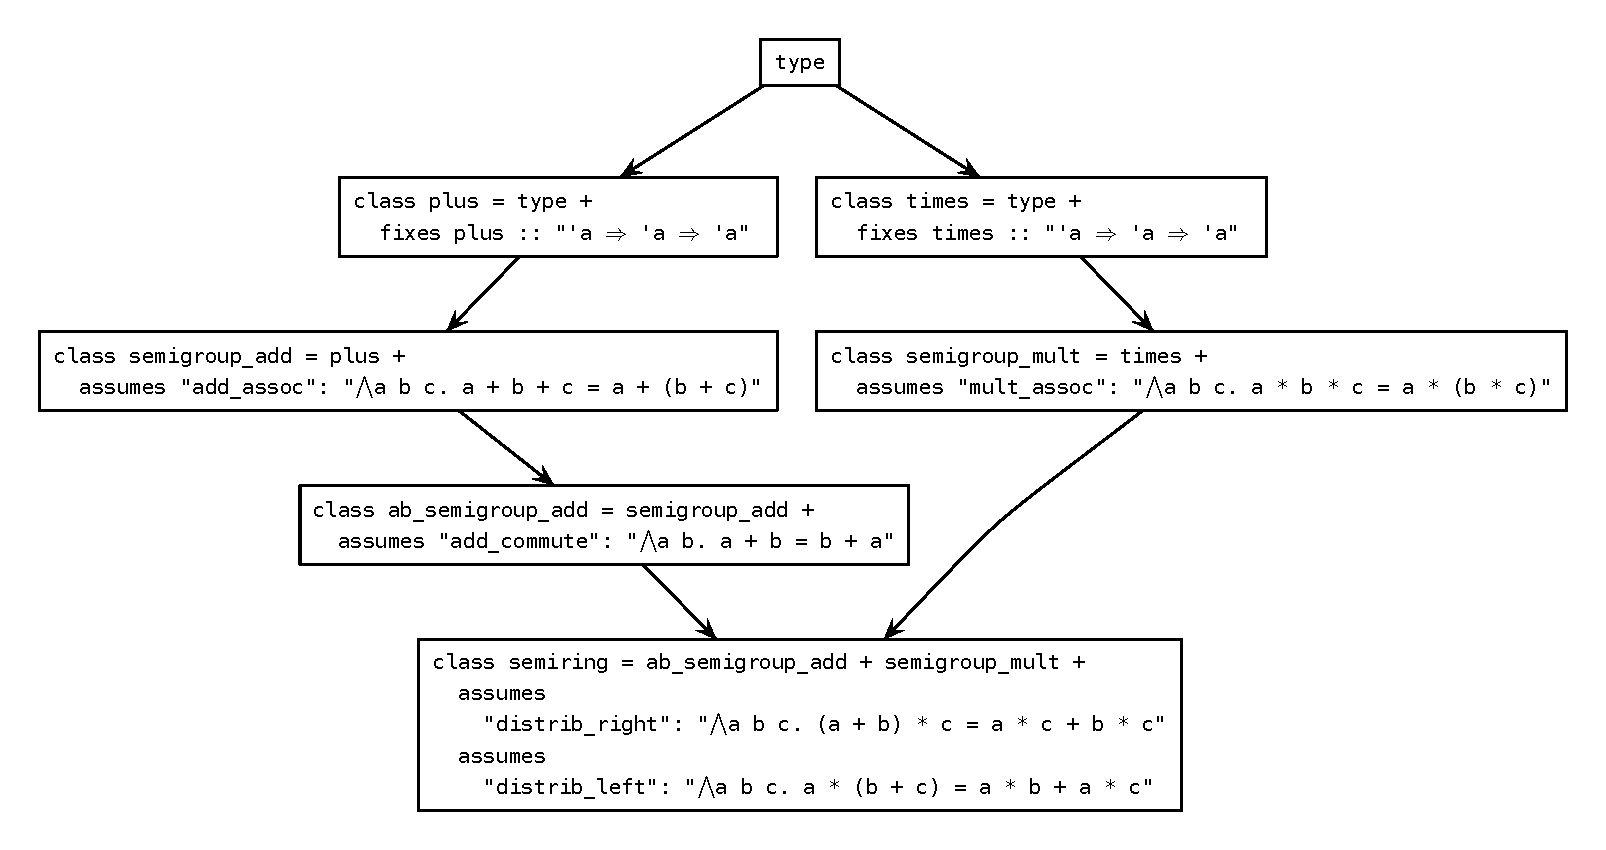
\includegraphics[width=\linewidth]{img/class-deps.pdf}
  \caption{Class hierarchy for the \holclass{comm\_semigroup\_add} class}
  \label{fig:preproc:hierarchy}
\end{figure}

\subsubsection{Superclass paths}

The class hierarchy in HOL is rather complex.
An excerpt, relating to the running example, is reproduced in \cref{fig:preproc:hierarchy}.
For example, to obtain the \holconst{plus} operation from a \holclass{semiring} constraint, one has to follow three subclass--superclasses edges.

In general, for any two classes $c$ and $d$, there may be multiple different paths from the subclass $c$ and the (possibly indirect) superclass $d$.
It is not obvious that the choice of path is irrelevant for the semantics of the generated program, i.e., that the system is \emph{coherent} according to Jones~\cite{jones1994types}. Isabelle's type system guarantees coherence \cite{nipkow1991typeclasses,nipkow1995reconstruction}, which the dictionary construction assumes.
If that assumption were violated, the equivalence proof (§\ref{sec:preproc:dict:equiv}) would fail.
Coherence is consequently a meta-theorem and not internalised in the logic.

For the purpose of this presentation, it is sufficient to assume that the implementation uses the ``first'' path according to the kernel-defined order of superclasses.
It is straightforward to extend the notation $\holtypejudgement{\dictinst{c \leadsto d}}{\alpha\;\holconst{dict\_}c \Rightarrow \alpha\;\holconst{dict\_}d}$ for an indirect superclass $d$ of $c$, where the edges are conjoined using the function composition operator $\circ$.

\subsubsection{Non-class constants}

Class constants can be easily distinguished from non-class ones:
The former have no defining equations.
They are only given meaning by an instance of a class.

In the example in \cref{fig:preproc:graph}, the constants \holconst{f}, \holconst{g} and \holconst{plus\_nat} are non-class constants, whereas \holconst{plus} is a class constant.
This is reflected in the graph: the box for \holconst{plus} has no defining equations.
Note that while \holconst{plus\_nat} participates in the instantiation of a type class, it is itself not considered to be a class constant.

Assume a transformation of a non-class constant $f$ with a set of defining equations $\mathit{eq}_i$.
Each of the $\mathit{eq}_i$ is of the form $f\;p_{i,1}\;p_{i,2}\;\ldots\;p_{i,n_i} \equiv \mathit{rhs}_i$, with the $p_{i,j}$ being constructor patterns.
Furthermore, the type of $f$ is a type scheme, i.e., it is of the form $\forall \holtypejudgement{\alpha_1}{s_1} \ldots \forall \holtypejudgement{\alpha_k}{s_k}.\; \tau$.
Each of the schematic type variables $\alpha_i$ may carry a sort constraint $s_i = \{ c_{i,1}, \ldots, c_{i,m_i} \}$ that is assumed to be normal.

Let $\dict{t}_\Gamma$ denote the translation of terms in a context $\Gamma$ (to be defined later).
Also, let \dictinst{f} mean a fresh name, e.g.\ $f'$ to refer to the newly defined constant.

I can now explain the translation of the defining equations.
Each equation $\mathit{eq}_i$ gives rise to a new equation $\dict{\mathit{eq}_i}$ as follows:
\begin{itemize}
  \item For every class constraint of every type variable, a new parameter is introduced.
  \item The existing parameters stay unchanged, because data constructors do not participate in the dictionary construction.
  \item The right-hand side is translated with all new parameters as context.
\end{itemize}

\noindent
Formally:
\begin{align*}
  \dict{\mathit{eq}_i} &= (\mathit{lhs}'_i \equiv \dict{\mathit{rhs}_i}_\Gamma) \\
  \Gamma &= [ \mathit{dict}\_c_{1,1}, \ldots, \mathit{dict}\_c_{k,m_k} ] \\
  \mathit{lhs}'_i &= \dictinst{f}\;(\holtypejudgement{\mathit{dict}\_c_{1,1}}{\alpha_1\;\holconst{dict}\_c_{1,1}})\;\ldots\;(\holtypejudgement{\mathit{dict}\_c_{k,m_k}}{\alpha_k\;\holconst{dict}\_c_{k,m_k}})\;p_{i,1}\;p_{i,2}\;\ldots\;p_{i,n_i}
\end{align*}

\noindent
Note that the translation for left-hand and right-hand sides differs:
left-hand sides, consisting only of patterns, need no context.

All resulting equations are considered as defining equations for \dictinst{f}.
Subsequently, they are fed into the internal interface of the \holcommand{function} command to produce a new logical constant.
The additional technical challenges of this are documented in the following sections.

\subsubsection{Instance definitions and composition}

An instance $\holtypejudgement{\kappa}{(s_1, \ldots, s_k)\;c}$ is treated as if it is a (non-class) constant with no arguments, returning a dictionary containing instantiations of all class constants.
Consequently, each instance gives rise to a new definition that I refer to as $\dictinst{\holtypejudgement{\kappa}{c}}$.

However, it is also necessary to compose instances from contexts.
This might mean a combination of following along superclass paths and applying instance definitions to arguments.
I use $\dict{\holtypejudgement{\tau}{c}}_\Gamma$ as notation for this, where $\tau$ is a simple type and $\Gamma$ a context.

I will first describe the (deterministic) algorithm to obtain $\dict{\holtypejudgement{\tau}{c}}_\Gamma$.
\begin{enumerate}
  \item
    If $\tau$ is a type variable, find an instance $\mathit{dict}$ for $\holtypejudgement{\tau}{c'}$  in $\Gamma$ where $c'$ is a subclass of $c$.
    Then, $\dict{\holtypejudgement{\tau}{c}}_\Gamma = \dictinst{c' \leadsto c}\;\mathit{dict}$.
  \item
    Otherwise, $\tau$ is of the form $(\tau_1, \ldots, \tau_k)\;\kappa$, i.e., a $k$-ary type constructor $\kappa$ applied to $k$ types.
    Find an instance definition $\holtypejudgement{\kappa}{(s_1, \ldots, s_k)\;c'}$ where:
    \begin{itemize}
      \item $c'$ is a subclass of $c$ and
      \item for each constraint $\holtypejudgement{\tau_i}{c_{i,j}}$ stemming from the $s_i$, $r_{i,j} = \dict{\holtypejudgement{\tau_i}{c_{i,j}}}_\Gamma$ is defined
    \end{itemize}
    Then, $\dict{\holtypejudgement{\tau}{c}}_\Gamma = \dictinst{c' \leadsto c}\;(\dictinst{\holtypejudgement{\kappa}{c'}}\;r_{1,1}\;\ldots\;r_{k,m_k})$.
  \item
    If no suitable instance exists, fail.
\end{enumerate}

\noindent For any well-sorted judgement $\holtypejudgement{\tau}{c}$, this algorithm is guaranteed to find at least one composed instance.
Similar to finding superclass paths, the choice of instance is irrelevant.
This is a meta-theorem based on the \emph{coregularity} property that is guaranteed by Isabelle's type system \cite{nipkow1991typeclasses,nipkow1995reconstruction}.

It remains to treat instance definitions $\dictinst{\holtypejudgement{\kappa}{c}}$.
Assuming the same naming conventions as above, the generated definition is of the following form:
\[
  \dictinst{\holtypejudgement{\kappa}{c}}\;\mathit{dict}_{1,1}\;\ldots = \holconst{mk\_}c\;\dict{\holtypejudgement{(\alpha_1, \ldots, \alpha_k)\;\kappa}{c_1}}_\Gamma\;\ldots\;\;\dict{\holtypejudgement{(\alpha_1, \ldots, \alpha_k)\;\kappa}{c_n}}_\Gamma\;\dict{f_1}_\Gamma\;\ldots\;\dict{f_m}_\Gamma
\]

\subsubsection{Terms}

I define the translation of terms \dict{t} that are not constants recursively as follows:
\begin{align*}
  \dict{x}_\Gamma &= x &\text{(where $x$ is a variable)} \\
  \dict{t\;u}_\Gamma &= \dict{t}_\Gamma\;\dict{u}_\Gamma \\
  \dict{\lambda x.\,t}_\Gamma &= \lambda x.\,\dict{t}_\Gamma
\end{align*}
The rule for constants is a bit more involved.
Let $f$ be a constant with $k$ type parameters, i.e., of type scheme $\forall \holtypejudgement{\alpha_1}{s_1} \ldots \forall \holtypejudgement{\alpha_k}{s_k}$.
In any occurrence of $f$ in a term, these type parameters are instantiated with simple types $\tau_1, \ldots, \tau_k$.
\[
  \dict{f}_\Gamma = \dictinst{f}\;\dict{\holtypejudgement{\tau_1}{c_{1,1}}}_\Gamma\;\ldots\;\dict{\holtypejudgement{\tau_k}{c_{k,m_k}}}_\Gamma
\]

\subsubsection{Challenges}

In the standard case, where the user has not performed a custom code setup, the resulting function looks similar to its original definition.
But the user may have also changed the implementation of a function significantly afterwards.
This poses some challenges:

\begin{itemize}
  \item
    The new constants need to be proven terminating.
    The routine heuristically transfers the original termination proof to the new definitions (§\ref{sec:preproc:dict:termination}).
    This only works when the termination condition does not rely on class axioms.
  \item
    The domain of functions must be tracked, because even though HOL is a total logic, functions may be under-specified.
    Congruence rules are used to construct an inductive predicate (§\ref{sec:background:inductive}) representing the \emph{side condition} of a function (§\ref{sec:preproc:dict:partial}).
  \item
    In order to fine-tune executable code, the code generator allows users to specify different constructors of a datatype than those it has been defined with, or even to introduce constructors for non-datatypes.
    However, the \holcommand{function} command does not support that in general (§\ref{sec:preproc:limitations}).
    But even if it did, the equivalence of old and new definition may become conditional on invariants, which is conceptually not supported (§\ref{sec:preproc:limitations}).
  \item
    The set of defining equations must be non-overlapping to ensure determinism.
    Additionally, to accommodate for later phases in the compiler (§\ref{sec:intermediate:elim}), some pattern variables need to be renamed (§\ref{sec:preproc:compatibility}).
\end{itemize}


\subsection{Preservation of termination}
\label{sec:preproc:dict:termination}

\begin{code}[t]
  \begin{lstlisting}
fun f :: nat $\Rightarrow$ nat where
f $0$ = $0$
f (Suc //n//) = f //n//

lemma [code]: f //x// = f //x// by simp\end{lstlisting}
  \caption{Pathological example of a non-terminating defining equation}
  \label{code:non-terminating}
\end{code}

As indicated above, the newly defined functions must be proven terminating.
In general, I cannot reuse the original termination proof, as the example in \cref{code:non-terminating} illustrates.
While the original function is primitively recursive, and hence trivially proved to be terminating, the user has added a defining equation that characterizes a non-terminating implementation.
My construction cannot deal with such pathological cases, but fortunately they are rare in practice.
The invocation of the dictionary construction would just fail for this example.

Instead, based on my experience, the most common cases are that users either
\begin{itemize}
  \item do not adapt the defining equations at all,
  \item adapt them without changing the termination scheme, or
  \item adapt them to use different recursive calls, while still being terminating.
\end{itemize}

\noindent
For the last case, it is impossible to port the existing termination proof, because it is not applicable any more.
Hence, the construction falls back to use the same automated proof method as the \holcommand{function} package.

However, the other cases are more interesting.
In the remainder of this section, I will illustrate the first case, which is a specialization of the second one.%
\thyrefafp{Dict_Construction}{Termination}
The original termination proof should intuitively be still applicable.

The running example will be a function that sums up values in a list.
%
\begin{lstlisting}
fun sum_list :: $\alpha$::{plus,zero} list $\Rightarrow$ $\alpha$ where
sum_list [] = //0//
sum_list (//x// # //xs//) = //x// + sum_list //xs//
\end{lstlisting}
%
This function carries two distinct class constraints -- arising from the use of addition and zero, both of which are provided by a class in Isabelle -- which are translated into two dictionary parameters:
%
\begin{lstlisting}[language=Isabelle]
sum_list' //dict_plus// //dict_zero// [] =
    const_zero //dict_zero//
sum_list' //dict_plus// //dict_zero// (//x// # //xs//) =
    const_plus //dict_plus// //x// (sum_list' //dict_plus// //dict_zero// //xs//)
\end{lstlisting}
%
Here, the termination argument has not changed:
While two additional parameters have been introduced, they remain unchanged in between recursive calls.
Observe that whenever sort constraints are present, the dictionary construction always introduces new arguments, but keeps the termination scheme.

Now, the termination of \holconst{sum\_list'} must be proved.
The \holcommand{function} package analyses the structure of recursive calls and collects them into a set of constraints.

As a notation for constraints, I will use $\bar{p} \leadsto \bar{x}$.
$\bar{p}$ stands for the (tupled) patterns on the left-hand side of an equation and $\bar{x}$ for the (also tupled) actual parameters passed to a recursive invocation.
Only variables bound in $\bar{p}$ may appear in $\bar{x}$.

\remark*{
  The \holcommand{function} command not only tracks the parameters passed to a recursive call, but also, under which conditions such a call appears.
  For example, a recursive call may appear in a \holkeyword{then} or \holkeyword{else} branch.
  To properly represent that, the notation needs to be extended to allow for arbitrary predicates.
  For explaining the termination heuristics, this generality is not needed; but it will be revisited for another purpose in §\ref{sec:preproc:dict:partial}.
}

\noindent
For the above example, this looks as follows:
%
\begin{align}
  \{ (x \cons \mathit{xs}) &\leadsto \mathit{xs} \} \tag{\holconst{sum\_list}} \\
  \{ (\mathit{dict\_plus}, \mathit{dict\_zero}, x \cons \mathit{xs}) &\leadsto (\mathit{dict\_plus}, \mathit{dict\_zero}, \mathit{xs})\} \tag{\holconst{sum\_list'}}
\end{align}
%
Internally, for every function $\holtypejudgement{f}{\sigma_1 \Rightarrow \sigma_2 \Rightarrow \ldots \Rightarrow \sigma_n \Rightarrow \tau}$, the package defines an inductive relation $\holtypejudgement{f\_\holconst{rel}}{(\sigma_1, \sigma_2, \ldots, \sigma_n) \Rightarrow (\sigma_1, \sigma_2, \ldots, \sigma_n) \Rightarrow \holtype{bool}}$ with one introduction rule per constraint.
Note that the arguments are tupled, i.e.\ all function arguments participate in the definition of this \emph{termination relation.}

In the example, the predicate \holconst{sum\_list\_rel} is defined by the following introduction rule:
\[
  \inferrule*{ }{
    \holconst{sum\_list\_rel}\;\mathit{xs}\;(x \cons \mathit{xs})
  }
\]

\noindent
For details on how the \holcommand{function} package assembles the termination relation based on the constraints, in particular for more complicated recursion schemes, refer to Krauss' thesis~\cite{krauss2009fun}.

To prove that a function terminates, it is sufficient to show that its termination relation is \emph{well-founded.}
In the majority of cases, this happens by supplying a suitable \emph{measure function} that maps the arguments to natural numbers and decreases for each recursive call.
The \holcommand{function} package is able to try out various measure functions automatically.

In this setting however, the termination of $f$ has already been proved, either automatically or by the user.
The construction tries to re-use that proof, i.e., the well-foundedness theorem of $f\_\holconst{rel}$, for the proof of well-foundedness of $f'\_\holconst{rel}$, where $f'$ is the result of applying the dictionary construction to $f$.
Except for the additional (unchanging) dictionary arguments, these relations are more or less equivalent to each other.

\begin{lemma}[Well-founded simulation]
  Let $\holtypejudgement{P}{\tau \Rightarrow \tau \Rightarrow \holtype{bool}}$ be a well-founded relation and $\holtypejudgement{g}{\sigma \Rightarrow \tau}$ a function such that
  \[
    \forall x\; y.\; P'\;x\;y \implies P\;(g\;x)\;(g\;y)
  \]
  Then, $\holtypejudgement{P'}{\sigma \Rightarrow \sigma \Rightarrow \holtype{bool}}$ is also a well-founded relation.
\end{lemma}

\begin{figure}[t]
  \centering
  \tikzstyle{r} = [circle, fill=gray!10, text width=1.5em, text height=1em, text centered, node distance=2cm]
  \tikzstyle{rprime} = [circle, fill=gray!30, text width=1.5em, text height=1em, text centered, node distance=2cm]
  \tikzstyle{simline} = [draw, -latex', densely dashed, thick]
  \tikzstyle{line} = [draw, -latex]

  \begin{tikzpicture}
    \node [r] (rx1) {$x_1$};
    \node [r, right of=rx1] (rx2) {$x_2$};
    \node [r, right of=rx2] (rx3) {$x_3$};
    \node [left of=rx1, node distance=2cm] {$P$};
    \node [right of=rx3, node distance=1.5cm] (rx4) {$\ldots$};

    \node [rprime, below of=rx1, node distance=3cm] (rpx1) {$x_1'$};
    \node [rprime, right of=rpx1] (rpx2) {$x_2'$};
    \node [rprime, right of=rpx2] (rpx3) {$x_3'$};
    \node [left of=rpx1, node distance=2cm] {$P'$};
    \node [right of=rpx3, node distance=1.5cm] (rpx4) {$\ldots$};

    \path [simline] (rpx1) -- (rx1) node [midway, right] {$g$};
    \path [simline] (rpx2) -- (rx2) node [midway, right] {$g$};
    \path [simline] (rpx3) -- (rx3) node [midway, right] {$g$};
    \path [line] (rx1) -- (rx2);
    \path [line] (rx2) -- (rx3);
    \path [line] (rx3) -- (rx4);
    \path [line] (rpx1) -- (rpx2);
    \path [line] (rpx2) -- (rpx3);
    \path [line] (rpx3) -- (rpx4);
  \end{tikzpicture}
  \caption{Well-founded simulation}
  \label{fig:preproc:dict:wfsim}
\end{figure}

\noindent
This theorem allows to \emph{simulate} the structure of the recursive calls of $f'$ with those of $f$ (depicted in \cref{fig:preproc:dict:wfsim}).
There is an important difference, though: $f\_\holconst{rel}$ may have sort constraints, $f'\_\holconst{rel}$ does not.

Instantiating the above lemma with the two termination relations entails choosing a suitable function $g$ that maps arguments of \holconst{sum\_list'} to arguments of \holconst{sum\_list}, i.e., a function of type
\[ (\alpha\;\holtype{dict\_plus} \times \alpha\;\holtype{dict\_zero} \times \alpha\;\holtype{list}) \Rightarrow (\holtypejudgement{\beta}{\{ \holclass{plus}, \holclass{zero} \}}) \;\holtype{list} \]
for an arbitrary type $\beta$.
Obviously, $g$ can drop the first two elements of the tuple.
The challenge arises when trying to map a list with element type $\alpha$ to one with element type $\beta$.
I cannot instantiate $\beta = \alpha$, because $\beta$ carries a sort constraint.

In a parametric setting, this would be the end of it, because it is impossible to write such a function~\cite{reynolds1983parametric,lochbihler2016probabilistic,gilcher2017parametricity}.
Isabelle however offers an escape hatch: recall that all types are non-empty.
The polymorphic constant $\holtypejudgement{\holconst{undefined}}{\alpha}$\holconstindex{undefined} can serve as a witness for an arbitrary type.
Assuming that there is at least one concrete type $\tau$ that satisfies the sort constraints of $\beta$, I can instantiate $\beta = \tau$.
The desired mapping function can now be specified as follows:
\[ g\;(\_, \_, \mathit{xs}) = \holconst{map}\;(\lambda \_.\;\holtypejudgement{\holconst{undefined}}{\tau})\;\mathit{xs} \]
In case there is no such concrete $\tau$, the above expressions fails to type check, causing the heuristic to fail.%

It remains to show how the premise of the well-founded simulation theorem is proved in this particular case:
\[
  \forall x\; y.\; \holconst{sum\_list'\_rel}\;x\;y \implies \holconst{sum\_list\_rel}\;(g\;x)\;(g\;y)
\]
The proof proceeds by induction using the induction principle of the \holconst{sum\_list'\_rel} inductive predicate, which gives one case per introduction rule, that is:
\[
  \forall \mathit{d\_plus}\;\mathit{d\_zero}\;x\;\mathit{xs}.\;\holconst{sum\_list\_rel}\;(g\;(\mathit{d\_plus}, \mathit{d\_zero}, \mathit{xs}))\;(g\;(\mathit{d\_plus}, \mathit{d\_zero}, x \cons \mathit{xs}))
\]
After unfolding the definition of $g$:
\[
  \forall \mathit{xs}.\;\holconst{sum\_list\_rel}\;(\holconst{map}\;(\lambda \_.\;\holconst{undefined})\;\mathit{xs})\;(\holconst{undefined}\cons \holconst{map}\;(\lambda \_.\;\holconst{undefined})\;\mathit{xs})
\]
This can now trivially be proved by using the introduction rule of \holconst{sum\_list\_rel}.

\remark*{
  This construction critically depends on the non-emptiness of types and that there is at least one type satisfying the sort constraints of a function.
  In that sense, it only works because HOL admits non-parametric definitions~\cite{reynolds1983parametric,lochbihler2016probabilistic,gilcher2017parametricity}.
}

\noindent
More generally, this construction allows the proof of well-foundedness of any relation
\[\holtypejudgement{R'}{(\beta_1 \times \ldots \times \beta_n \times (\alpha_1, \ldots, \alpha_k)\;\tau) \Rightarrow (\beta_1 \times \ldots \times \beta_n \times (\alpha_1, \ldots, \alpha_k)\;\tau) \Rightarrow \holtype{bool}}\]
given a well-founded relation
\[\holtypejudgement{R}{(\alpha_1, \ldots, \alpha_k)\;\tau' \Rightarrow (\alpha_1, \ldots, \alpha_k)\;\tau' \Rightarrow \holtype{bool}}
\]
where $\tau$ is a suitable type constructor equipped with a functorial $\holconst{map}_\tau$, $\tau$ and $\tau'$ differ only in sort constraints, $R$ and $R'$ are structurally equivalent and parametric in all $\alpha_i$.

\remark*{
  The precise nature of ``suitability'' is not relevant for the discussion.
  In the implementation, bounded natural functors as introduced by Blanchette~\etal~\cite{blanchette2017bnf,blanchette2014datatypes} without dead variables are considered suitable.
}

\noindent
The mapping function $g$ is defined as follows:
\begin{align*}
  &\holtypejudgement{g}{(\beta_1 \times \ldots \times \beta_n \times (\alpha_1, \ldots, \alpha_k)\;\tau) \Rightarrow (\alpha_1, \ldots, \alpha_k)\;\tau'} \\
  &g\;(\_, \ldots, \_, t) = \holconst{map}_\tau\;\underbrace{(\lambda \_.\; \holconst{undefined})\;\ldots\;(\lambda \_.\; \holconst{undefined})}_{\text{one for each $\alpha_i$}}\;t
\end{align*}

\subsection{Partially specified functions}
\label{sec:preproc:dict:partial}

HOL is a total logic, that is, it is always possible to assign a value to a function $\holtypejudgement{f}{\alpha \Rightarrow \beta}$ applied to any argument $\holtypejudgement{x}{\alpha}$.
This immediately raises the question how to represent \emph{partially specified} (or \emph{under-specified}) functions, e.g.\ to obtain the head of a list:
%
\begin{lstlisting}[language=Isabelle]
fun hd :: $\alpha$ list $\Rightarrow$ $\alpha$ where
hd (//x// # //xs//) = //x//
\end{lstlisting}
%
Obviously, in this function definition, the case for the empty list is omitted.
Note that under-specification and non-termination are different kinds of partiality; the latter of which is not supported by this work.

\remark*{
  It is possible to define and reason about non-terminating functions in Isabelle.
  However, both the dictionary construction and the deep embedding steps~(§\ref{sec:deep}) are unable to process such definitions.
  Other steps of the pipeline, in particular the verified part~(§\ref{sec:compiler}), do not presuppose termination of the original equations.
}

\noindent
There are various ways to deal with under-specification (a more detailed survey is given in §\ref{sec:preproc:dict:related}):

\begin{enumerate}
  \item
    Lift the result type into \holtype{option}, i.e.\ $\alpha \Rightarrow \beta$ turns into $\alpha \Rightarrow \beta\;\holtype{option}$.
    Arguments for which the function is not specified get assigned a \holconst{None} value.
    The domain of the function $\holconst{dom}_f$ can conveniently be expressed as a set $\{ x \mid f\;x \neq \holconst{None} \}$.
  \item
    Function definitions are ``artificially'' completed to be always specified.
    In HOL, \holconst{undefined} is an unspecified constant of arbitrary type.
    The meta-theorem about this unspecified constant is that for all predicates $P$, $P\;\holconst{undefined}$ is provable if and only if $P\;x$ is provable for all $x$.
  \item
    Based on the function equations, derive a set carrying the \emph{side condition} of the function and allow reasoning over a function application $f\;x$ only if $x \in \holconst{side}_f$ holds.
    This is comparable to refinement types \cite{gordon2010refinement}, but where the constraints are external and not part of the type.
\end{enumerate}

\noindent
I will examine the specification of the \holconst{hd} function for each of the different approaches.

\paragraph{Lifting}
This approach is preferred in many functional programming languages, like Haskell, where types may be non-empty (ignoring exceptions).
The major problem is that it may lead to complicated proof statements when reasoning about such functions.
%
\begin{lstlisting}[language=Isabelle]
fun hd :: $\alpha$ list $\Rightarrow$ $\alpha$ option where
hd (//x// # //xs//) = Some //x//
hd [] = None
\end{lstlisting}
%
In this setting, this would require non-trivial transformation of existing defining equations.
Wimmer \etal~\cite{wimmer2018memoization} solve a similar problem in the context of memoization: they lift functions into the state monad.
The main weakness is that higher-order functions need to be lifted manually.
Because many existing Isabelle formalizations make use of custom combinators, their approach is not feasible here.

\paragraph{Completion}
Isabelle's \holcommand{function} package uses this approach by default.
For any given function definition, a catch-all clause is added (a process called \emph{completion}):
%
\begin{lstlisting}[language=Isabelle]
fun hd :: $\alpha$ list $\Rightarrow$ $\alpha$ where
hd (//x// # //xs//) = //x//
hd _ = undefined
\end{lstlisting}
%
As far as the \holcommand{function} package is concerned, this function is now specified for all input values.

To avoid leaking this implementation detail to users, Isabelle's simplifier will not rewrite the term $\holconst{hd}\;[]$ to \holconst{undefined}.
But the completion is visible in the generated induction principle \holthm{hd.induct}:
\[
  \inferrule*{
    \forall x\;\mathit{xs}.\;P\;(x \cons \mathit{xs}) \\
    P \; []
  }{P\;a}
\]
The premise $P\;[]$ is necessary for this theorem to hold.
Otherwise, $P\;\mathit{xs} = (\mathit{xs} \neq [])$ would be a counterexample.

While this approach is conceptually simple, it poses a significant challenge for the dictionary construction and associated proof tactics.
The reason is as profound as it is technical:
Applications of functions to values on which they are not specified are practically ``opaque''; in the sense that it is difficult to rewrite or prove anything about them.
To make matters worse, identities like $\holconst{undefined}\;x = \holconst{undefined}$ are unprovable, meaning \holconst{undefined} behaves differently than e.g.\ $\bot$ in Haskell (where $\bot\;x = \bot$ holds).
It is hence an insufficient approximation of under-specification for the purposes of code generation.

\paragraph{Side conditions}
To avoid modifying the internal mechanics of the \holcommand{function} package, and consistent with Myreen and Owens' approach \cite{myreen2014translation}, I have chosen to track side conditions of functions.
They are represented as inductive predicates.
In the case of the head function, the predicate is specified as follows:
\[
  \inferrule*{ }{\holconst{hd\_side}\;(x \cons \mathit{xs})}
\]

\noindent
When producing a certificate for the dictionary translation (§\ref{sec:preproc:dict:elim:cert}) for an under-specified function \holconst{f}, the routine introduces a new premise:
\[ \holconst{cert\_plus}\;\mathit{dict} \implies \holconst{f\_side}\;x \implies \holconst{f'}\;\mathit{dict}\;x = \holconst{f}\;x \]
A more subtle change is that the theorem now has to be stated in $\eta$-expanded form.
This may limit its applicability in higher-order position, e.g.\ $\holconst{map}\;\holconst{f}$.

Before describing the construction of the inductive predicates for side conditions, I will rehash the concept of \emph{congruence rules}.

\subsubsection{Congruence rules}
\label{sec:preproc:dict:partial:cong}

The notion of \emph{congruence rules}\index{congruence rule} goes back to the literature on term rewriting~\cite{felty1992rewriting,felty1992conditional}.
Later, they have become instrumental in the context of admitting recursive definitions in higher-order logics~\cite{slind1999terminating,krauss2009fun,krauss2010recursive}.

\begin{definition}[Congruence rule]
  A \emph{congruence rule} for the function \holconst{c} is a theorem of the form
  \[
    \inferrule{
      P_1 \\
      \cdots \\
      P_n
    }{
      \holconst{c}\;x_1\;\ldots\;x_n = \holconst{c}\;y_1\;\ldots\;y_n
    }
  \]
  where the $P_i$ may refer to arbitrary $x_i$ and $y_i$.
\end{definition}

\noindent
Usually, the $P_i$ takes either of these two forms:
\begin{itemize}
  \item $Q_i \implies x_i = y_i$, when $\holtypejudgement{x_i}{\tau}$ and $\tau$ is not a function type
  \item $\forall \bar{z}.\;Q_i\;\bar{z} \implies x_i\;\bar{z} = y_i\;\bar{z}$, otherwise
\end{itemize}

\noindent
Slind \cite[§2.7.1]{slind1999terminating} calls a congruence rule where no functions are passed as arguments \emph{simple}.
Two examples of those are given below:

\[
  \inferrule*{
    C_1 = C_2 \\
    C_1 \implies x_1 = x_2 \\
    \neg C_1 \implies y_1 = y_2
  }{
    \holkeyword{if}\;C_1\;\holkeyword{then}\;x_1\;\holkeyword{then}\;y_1 =
    \holkeyword{if}\;C_2\;\holkeyword{then}\;x_2\;\holkeyword{then}\;y_2
  }
\]
\[
  \inferrule*{
    A_1 = A_2 \\
    A_1 \implies B_1 = B_2
  }{
    A_1 \wedge B_1 = A_2 \wedge B_2
  }
\]

\noindent
The purpose of these rules is to track \emph{evaluation context.}
This is important because HOL itself has no notion of evaluation order, but target languages do.
In particular, both in Slind's \holcommand{recdef} and Krauss' \holcommand{function} package, congruence rules are used to determine the termination relation of a function.
Both take the $Q_i$ of the rules into account to guard recursive invocations, like in the following example:
%
\begin{lstlisting}[language=Isabelle]
fun fac :: nat $\Rightarrow$ nat where
fac //n// = (||if|| //n// = $0$ ||then|| $1$ ||else|| //n// * fac (//n// - $1$))
\end{lstlisting}
%
A naive termination analysis would complain that \holconst{fac} never terminates, because there is always a recursive call.
The \holcommand{function} package however derives the following termination relation:

\[
  \inferrule*{n \neq 0}{\holconst{fac\_rel}\;(n - 1)\;n}
\]

\noindent
This is clearly well-founded, i.e.\ \holconst{fac} terminates on all inputs, because there is no $n'$ such that $\holconst{fac\_rel}\;n'\;0$.

Extending the notation from §\ref{sec:preproc:dict:termination} with arbitrary conditions, the above relation can be more succinctly expressed as:
\[
  \{ n \stackrel{n \neq 0}{\leadsto} (n-1) \}
\]

\noindent
More complex cases arise when higher-order recursion is present.
Consider this datatype and function:
%
\begin{lstlisting}[language=Isabelle]
datatype $\alpha$ tree = Fork ($\alpha$ tree list) | Leaf $\alpha$

fun map_tree where
map_tree //f// (Fork //ts//) = Fork (map (map_tree //f//) //ts//)
map_tree //f// (Leaf //x//) = Leaf (//f// //x//)
\end{lstlisting}
%
It takes more work to understand this \emph{nested} recursion principle.
It is not directly obvious on which values \holconst{map\_tree} is called recursively, because it only appears in partially applied form in the function body.
The \holcommand{function} package uses the higher-order congruence rule for \holconst{map} to deduce the termination relation:

\[
  \inferrule*{
    \forall x.\; x \in \holconst{set}\;\mathit{xs} \implies f\;x = g\;x\\
    \mathit{xs} = \mathit{ys}
  }{\holconst{map}\;f\;\mathit{xs} = \holconst{map}\;g\;\mathit{ys}}
\]

\noindent
Intuitively speaking, this represents the fact that the function passed to \holconst{map} is applied to each element in the set of $\mathit{xs}$, where $\holconst{set}$ is a function that turns a list into a set.
Consequently, the termination relation states exactly that:
%
\[
  \inferrule*{t \in \holconst{set}\;\mathit{ts}}{\holconst{map\_tree\_rel}\;(f, t)\;(f, \holconst{Fork}\;\mathit{ts})}
\]

\noindent
The $\leadsto$ notation starts to break down for this example, because the recursive call depends on a variable (here: $t$) that is not bound by the patterns of the defining equation (here: $\mathit{ts}$).
Consequently, in the remainder of this section, I will only use the rule-based notation to represent inductive predicates.

Well-foundedness can be proved by appealing to the size of the arguments.
The \holcommand{datatype} package provides a $\holconst{size}_\tau$ function for each type constructor $\tau$ that counts the number of data constructors in the value.
Consequently, if $t$ is an element of $\mathit{ts}$, then the size of $t$ is smaller than the size of $\holconst{Fork}\;\mathit{ts}$.

All of the necessary infrastructure for this is fully automated in Isabelle:
\begin{itemize}
  \item generation of $\holconst{map\_}\tau$ and $\holconst{set\_}\tau$ functions for datatypes and bounded natural functors $\tau$,
  \item proof of a suitable higher-order congruence rule,
  \item generation of $\holconst{size\_}\tau$ functions for datatypes $\tau$,
  \item setup of the \holcommand{function} package.
\end{itemize}

\noindent
The only occasion when a user has to adjust the setup is when they introduce a custom higher-order recursion combinator, or when a function definition uses a more complicated termination measure than the size of the inputs.

\subsubsection{Specifiedness}
\label{sec:preproc:dict:partial:spec}

Congruence rules can also be used to determine on which inputs functions are specified.
A similar routine as in the \holcommand{function} package can be employed to analyse function definitions.
Here, the goal is to construct an inductive predicate capturing the set of arguments for which a function is specified.

For example, consider the following (contrived) function definition:
\begin{lstlisting}[language=Isabelle]
fun hd_tl :: $\alpha$ list list $\Rightarrow$ $\alpha$ list
hd_tl [] = []
hd_tl (//x// # //xs//) = map hd //xs//
\end{lstlisting}

\noindent
The function itself has no obvious unspecified behaviour, because all possible inputs are covered by pattern matching.
However, the function \holconst{hd} is unspecified for empty lists.
The desired side condition is:

\[
  \inferrule*{
  }{\holconst{hd\_tl\_side}\;[]}\qquad
  \inferrule*{
    \forall x.\;x \in \holconst{set}\;\mathit{xs} \implies \holconst{hd\_side}\;x
  }{\holconst{hd\_tl\_side}\;(x \cons \mathit{xs})}
\]

\noindent
This can further be simplified by noting that $\holconst{hd\_side}\;x \biimplies x \neq []$.
This inductive definition can be obtained by performing a recursive analysis on the defining equations of a constant.
Each equation of \holconst{f} gives rise to a rule in \holconst{f\_side}.

Note that as far as Isabelle's total logic is concerned, this function is total:
The \holconst{hd} function just returns \holconst{undefined} on empty lists.
Because of this, any notion of \emph{specifiedness} cannot be fully formalized and has to be -- to some extent -- a heuristic.
A good intuition is that I want to characterize all inputs $x$ to a function $\holconst{f}$ such that evaluation after code generation to a target language does not yield a run-time exception.

\begin{code}[t]
  \begin{lstlisting}[language=ML]
type rule = {rule: thm, concl: term, prems: term list, proper: bool}

type ctx = (string * typ) list * term list

datatype ctx_tree = Tree of (term * (rule * (ctx * ctx_tree) list) option)
  \end{lstlisting}
  \caption{Type of context trees}
  \label{code:preproc:ctxtree}
\end{code}

\begin{figure}[t]
  \centering
  \tikzset{
    sibling distance=8em, level distance=5em,
    tree/.style = {shape=rectangle, draw, align=center, minimum height=2em, text depth=.25ex}
  }
  \begin{subfigure}[b]{.45\linewidth}
    \centering
    \begin{tikzpicture}
      \node [tree] (empty) {$[]$};
      \node [tree, right of=empty, node distance=4em] {$\holconst{map}\;\textcolor{Blue}{\holconst{hd}}\;\textcolor{OliveGreen}{\mathit{xs}}$}
        child [color=Blue] { node [tree] {$\holconst{hd}\;x$} edge from parent node [left, xshift=-1em, align=center] {$\holtypejudgement{x}{\alpha}$ \\ $x \in \holconst{set}\;\mathit{xs}$} }
        child [color=OliveGreen] { node [tree] {$\mathit{xs}$} };
    \end{tikzpicture}
    \caption{Forest with congruence rule for \holconst{map}}
    \label{fig:preproc:ctxtree:forest_with}
  \end{subfigure}
  \begin{subfigure}[b]{.53\linewidth}
    \small
    \[
      \inferrule*{
      }{\holconst{hd\_tl\_side}\;[]}
    \]
    \[
      \inferrule*{
        \holconst{map\_side}\;\holconst{hd}\;\mathit{xs}\\
        \forall x.\;x \in \holconst{set}\;\mathit{xs} \implies \holconst{hd\_side}\;x
      }{\holconst{hd\_tl\_side}\;(x \cons \mathit{xs})}
    \]
    \caption{Side condition with congruence rule for \holconst{map}}
    \label{fig:preproc:ctxtree:condition_with}
  \end{subfigure}
  \vspace{1em}

  \begin{subfigure}[b]{.45\linewidth}
    \centering
    \begin{tikzpicture}[sibling distance=6em]
      \node [tree] (empty) {$[]$};
      \node [tree, right of=empty, node distance=4em] {$\textcolor{BrickRed}{\holconst{map}}\;\textcolor{Blue}{\holconst{hd}}\;\textcolor{OliveGreen}{\mathit{xs}}$}
        child [color=BrickRed] { node [tree] {$\holconst{map}$} }
        child [color=Blue] { node [tree] {$\holconst{hd}$} }
        child [color=OliveGreen] { node [tree] {$\mathit{xs}$} };
    \end{tikzpicture}
    \caption{Forest without congruence rule for \holconst{map}}
    \label{fig:preproc:ctxtree:forest_without}
  \end{subfigure}
  \begin{subfigure}[b]{.53\linewidth}
    \small
    \[
      \inferrule*{
      }{\holconst{hd\_tl\_side}\;[]}
    \]
    \[
      \inferrule*{
        \holconst{map\_side}\;\holconst{hd}\;\mathit{xs}\\
        \textcolor{Brown}{\forall x.}\;\holconst{hd\_side}\;\textcolor{Brown}{x}
      }{\holconst{hd\_tl\_side}\;(x \cons \mathit{xs})}
    \]
    \caption{Side condition without congruence rule for \holconst{map}}
    \label{fig:preproc:ctxtree:condition_without}
  \end{subfigure}

  \caption{Context forests and resulting side conditions of \holconst{hd\_tl}}
  \label{fig:preproc:ctxtree}
\end{figure}

\paragraph{Transformation to forest}
The routine starts by importing the (unstructured) set of congruence rules into a dedicated data structure (\cref{code:preproc:ctxtree}).
Then, the right-hand sides of all defining equations are converted into a \emph{context tree.}
Each node of the tree is labelled with a term and optionally, a congruence rule, and may have arbitrarily many children.
An edge from a node to a child is labelled with a \emph{context:}
a list of variables and of assumptions.

\remark*{
  In usual Isabelle parlance, a ``context'' would refer to a \texttt{Proof.context} that may contain arbitrary data; in this case, it is just fixed variables and assumptions.
}

\noindent
An example based on the $\holconst{hd\_tl}$ function is given in \cref{fig:preproc:ctxtree}.
It illustrates how the congruence rule of \holconst{map} participates in the transformation.

The transformation algorithm itself can be summarized as follows.
For a term $t$, a node is generated.
Then, it adds children to the node by case distinction on the shape of $t$:
\begin{itemize}
  \item
    If $t$ is atomic, it becomes a leaf node.
  \item
    If $t$ is a function application $\holconst{f}\;x_1\;\ldots\;x_n$, it tries to find a congruence rule that matches the term.
    $k$ children are added to the node according to the $k$ premises of the rule, tracking their variables and assumptions as context of the respective child.
    If there is no matching rule, the function and its arguments are considered separately, hence creating $n+1$ children.
  \item
    Otherwise, $t$ is an abstraction $\lambda x.\;u$.
    One child for $u$ is added with $x$ as context.
\end{itemize}

\noindent
In \cref{fig:preproc:ctxtree:forest_with}, there are two trees.
\begin{itemize}
  \item $\holconst{hd\_tl}\;[] = []$ gives rise to the tree with just a leaf node $[]$, because $[]$ is an atomic constant.
  \item $\holconst{hd\_tl}\;(x \cons \mathit{xs}) = \holconst{map}\;\holconst{hd}\;\mathit{xs}$ produces a node with two children, after applying the congruence rule for \holconst{map}.
    The left child has a context enriched with a variable and assumption, whereas the right child is the atomic $\mathit{xs}$.
\end{itemize}

\noindent
Ignoring the congruence rule results in the forest in \cref{fig:preproc:ctxtree:forest_without}, where three children are generated for the binary call to \holconst{map}.

\paragraph{Transformation to predicate}
Finally, the tree is transformed into a set of introduction rules for the inductive predicate representing the specifiedness.
\cref{fig:preproc:ctxtree:condition_with} illustrates the result of the transformation.
In a tree, each path from root to the side condition generates one assumption in the side condition based on the pre-existing side conditions, unless:
\begin{itemize}
  \item it is the first child of a function application with no matching congruence rule (nothing is known about that function call), or
  \item it is a free variable (always specified), or
  \item no side condition is known about the term (assumed total).
\end{itemize}

\noindent
Crucially, each layer of the tree still contributes to the side condition.
In the running example, this means that the root node contributes the assumption $\holconst{map\_side}\;\holconst{hd}\;\mathit{xs}$.

A special case arises in \cref{fig:preproc:ctxtree:condition_without}, where an assumption is generated for the node \holconst{hd}.
Because the forest has been created without a suitable congruence rule, there is no variable in the context of the node.
The transformation hence introduces a synthetic variable and universally quantifies over it (marked brown in the figure).
It can be proved that $\forall x.\;\holconst{hd\_side}\;x$ is false, because there is a list that violates $\holconst{hd\_side}$: the empty list.
In general, absence of congruence rules or congruence rules that are too weak may lead to vacuous side conditions.

The side condition for \holconst{undefined} is a prime example for being vacuous by definition:
there are no defining equations, hence no context trees, hence the inductive predicate is the empty least-fixed point.
The \holcommand{inductive} package admits such empty predicates.
They are logically vacuous, i.e., $\holconst{undefined\_side} \biimplies \holconst{False}$.

\paragraph{Simplification}
To avoid overly complicated side conditions, there are two strategies to simplify them.
The routine tries to:
\begin{enumerate}
  \item prove totality, i.e.\ $\forall x_1 \ldots x_n.\;\holconst{f\_side}\;x_1\;\ldots\;x_n$, and
  \item discharge auxiliary side conditions, e.g.\ $\holconst{hd\_side}\;(x \cons \mathit{xs}) = \holconst{True}$.
\end{enumerate}

\noindent
Both work by suitable preprocessing of the goal, then running Isabelle's full simplifier.
While this can make the result unpredictable, I have found that this prevents many redundant assumptions.

For the example in \cref{fig:preproc:ctxtree}, this removes the assumption $\holconst{map\_side}\;\holconst{hd}\;\mathit{xs}$, because $\holconst{map\_side}$ can be proved to be total.

\remark*{
  It is important to note that the generated side conditions are \emph{shallow}, that is, they only characterize the specifiedness of one function, but not any other non-constant functions, i.e.\ functions that are passed in as parameters, that are called along the way.
  This is nicely illustrated by this example:
  While the \holconst{map} function is obviously fully specified, it can be used in a partially specified way; namely, when the mapping function is only partially specified.
  The challenges to fully capture specifiedness are described in §\ref{sec:preproc:limitations}.
}

\subsubsection{Differences to Krauss' routine}

As indicated above, the \holcommand{function} package employs a similar routine.
The differences are mainly technical in nature, but are significant enough to prevent code reuse.
\begin{itemize}
  \item
    The internally produced congruence tree is not exported as a data structure.
  \item
    Traversal happens on an intermediate constant that represents all functions in a mutually recursive bundle with tupled arguments.
    For example, simultaneous recursive definitions of \holconst{odd} and \holconst{even} functions would internally be presented as a single function of type $(\holtype{nat} + \holtype{nat}) \Rightarrow (\holtype{bool} + \holtype{bool})$, where $\alpha + \beta$ denotes the sum type of $\alpha$ and $\beta$.
  \item
    Side conditions of auxiliary constants (in the running example: \holconst{map} and \holconst{hd}) are not considered: after defining and proving a function to be terminating, it is ``total'' by virtue of completion.
\end{itemize}

\noindent
Notably, the extraction of a termination relation -- just like specifiedness -- critically depends on the presence of appropriate congruence rules.
Similarly to the special case described above, absence of congruence rules may lead to unprovable termination relations.
Consequently, it is reasonable to assume that a user of the \holcommand{function} package is aware of this required setup; hence, it is not an extra burden to require the same setup for the dictionary construction.

\subsection{Correctness proofs}
\label{sec:preproc:dict:equiv}

There are two kinds of propositions that need to be proved in the routine:
dictionary certificates and equivalence theorems (§\ref{sec:preproc:dict:elim:encoding}).
In general, they are of the form:
\begin{align*}
  \ldots &\implies \holconst{cert\_}c\;(\holconst{inst\_}c\holconst{\_}\kappa\;\mathit{dict}_1\;\ldots) \\
  \ldots &\implies \holconst{f'}\;\mathit{dict_1}\;\ldots\;x_1\;\ldots = \holconst{f}\;x_1\;\ldots
\end{align*}
Both can carry preconditions for auxiliary dictionary certificates, and in the case of the equivalence theorems, also side conditions of the arguments $x_i$ (§\ref{sec:preproc:dict:partial}).
The proof strategies for both kinds of theorems differ, so I will discuss them separately.
Both strategies have in common that they require the proofs to happen in exactly the same (topological) order as the dictionary construction itself (\cref{fig:preproc:graph}).
At any point during a sequence of proofs, the previous correctness theorems are referred to as \emph{base theorems.}

\paragraph{Dictionary certificates}
Recall the definition of $\holconst{cert}\_c$ and $\dictinst{\holtypejudgement{\kappa}{c}}$.
The latter is a plain constructor application ($\holconst{mk}\_c$); the former inspects each field.
In other words, $\dictinst{\holtypejudgement{\kappa}{c}}$ ``bundles'' existing constants into a dictionary.
Consequently, the proof proceeds by simple application of the base theorems.

\paragraph{Equivalence theorems}
In general, these theorems need to be proved by induction using the induction scheme generated by the side condition, or if the side condition is trivial, the termination relation of the function.
Both are similar, so I focus on the latter.

Applying the induction principle creates one proof obligation per defining equation.%
Recall the \holconst{sum\_list} function from §\ref{sec:preproc:dict:termination}.
The proof obligations after induction are (dictionary certificates omitted):
\begin{align*}
  \holconst{sum\_list'}\;\mathit{d}_1\;\mathit{d}_2\;[] &= \holconst{sum\_list}\;[] \\
  \holconst{sum\_list'}\;\mathit{d}_1\;\mathit{d}_2\;\mathit{xs} = \holconst{sum\_list}\;\mathit{xs} \implies \holconst{sum\_list'}\;\mathit{d}_1\;\mathit{d}_2\;(x\cons\mathit{xs}) &= \holconst{sum\_list}\;(x\cons\mathit{xs})
\end{align*}
These can be discharged by first unfolding the defining equations of \holconst{sum\_list'} and \holconst{sum\_list}.
Then, base theorems and induction hypotheses are applied by walking the congruence tree.
Note that the base theorems include equivalences for class constants and the corresponding dictionary fields.

\remark*{
  The reality is a bit more complicated:
  one equation may create multiple defining equations, because the \holcommand{function} command disambiguates equations.
  For example, consider the definition $\holconst{single}\;[x] = \holconst{True}$ and $\holconst{single}\;\mathit{xs} = \holconst{False}$.
  The package instantiates the second equation ($\mathit{xs} = y\cons\mathit{ys}$ and $\mathit{xs} = []$) to avoid ambiguities.
}

\subsection{Related work}
\label{sec:preproc:dict:related}

\paragraph{Dictionary construction}
Type classes have been pioneered by the Haskell programming language~\cite{morris2013classes,wadler1989adhoc}.
There, a very similar construction to here is used, replacing classes by records and instances by functions~\cite{peternson1993typeclasses,augustsson1993overloading,chen1992parametric}.
Additional complications arise because Haskell admits cyclic dependencies between class instances~\cite{laemmel2005syb}, which are prohibited in Isabelle and hence pose no problem for this work.
A further simplification compared with Haskell is that Isabelle only features an ML-style simply typed polymorphic lambda calculus without constructor or multi-parameter classes.

Idris, a dependently typed functional language, generalizes the concept of type classes to classes that can be parametrized by any value.
In more recent versions of Idris, they are called \emph{interfaces}.
Still, the elaboration of expressions with class constraints and class and instance declarations is surprisingly similar to here~\cite{brady2013idris}.

In Scala, type classes are represented in an object-oriented style with objects and implicits~\cite{oliveira2010typeclasses}.
Type classes are just regular classes that are subject to the same compilation process to the Java Virtual Machine (and other backends).
Instances are also regular functions and constraints regular function arguments.
However, programmers do not need to pass instances manually; the compiler fills them in automatically.
The end result again is similar to that of Haskell and Idris, albeit it is mostly visible in the surface syntax instead of hidden in some intermediate compiler representation.

For Isabelle, Haftmann and Nipkow give a pen-and-paper correctness proof of the dictionary construction construction \cite[§4.1]{haftmann2010codegeneration}, based on a notion of \emph{higher-order rewrite systems}.
The resulting theorem states that any well-typed term is reduction-equivalent before and after class elimination.
In this work, the dictionary construction is performed in a certified fashion, that is, the equivalence is a theorem inside the logic.

\paragraph{Partially specified functions}
The notion of functions that are not defined universally for all possible (i.e.\ type-correct inputs) is pervasive in programming languages.
For example, major functional languages, like Haskell, Scala, and OCaml admit introduction of unspecified behaviour by allowing incomplete pattern matches.
The respective run-time environments throw an exception which can be caught by the caller of an underspecified function.
This is not generally how it works in total logics, where it is impossible to carry out non-trivial proofs about unspecified values.

However, much work on modelling partiality in proof assistants is centred around partiality induced by non-termination, instead of under-specification.
Finn \etal~\cite{finn1997partial} introduce an approach for the \emph{LAMBDA} system that tackles both issues in a similar way as Isabelle/HOL.
The undefined or arbitrary constant can be defined in terms of Hilbert's choice operator: under the assumption that $\tau$ is inhabited, $\epsilon \holtypejudgement{x}{\tau}.\;\holconst{False}$ delivers a value of type $\tau$ that is otherwise unspecified.
The authors use a similar example (head of a list) and point out that the usual axioms of classical logic still apply; for example, $\holconst{hd}\;[] = 5 \vee \holconst{hd}\;[] \neq 5$ is provable regardless of the unspecified result of retrieving the head of an empty list.
They also give a routine that, given a set of recursive equations, defines a domain predicate and a function that is qualified on that predicate.
My approach (§\ref{sec:preproc:dict:partial:spec}) is similar to the one by Finn \etal, with the notable improvement that I support higher-order recursion.

Cheng and Jones~\cite{cheng1991usability} give a survey of the treatment of partial functions, with the focus on usability.
They examine a total of eight different approaches:
restricting functions to a set while defining them,
treating functions as relations,
employing a different notion of equality,
extending logical operators to handle undefined values,
three-valued logics,
introducing a distinction between strict and total and non-strict and non-commutative connectives,
introducing a distinction between computation and reasoning, and finally,
adding a separate judgement for definedness.
My approach is most closely related to the last of these, which has initially been described by Plotkin as \emph{Partial Function Logic}~\cite[§9]{cheng1991usability}.
The notable difference is that the definedness judgement is represented as ``normal'' boolean predicates in the logics.

% !TeX spellcheck = en_GB
% !TeX encoding = UTF-8

\section{Lazy evaluation}
\label{sec:preproc:lazy}

\authorship{
  Portions of this section appear in the AFP entry \citetitle{hupel2017lazycase}, authored by \citeauthor{hupel2017lazycase}~\cite{hupel2017lazycase}.
  Users are recommended to refer to that AFP entry for the latest documentation.
}

\noindent
HOL has no built-in notion of pattern matching.
Since my initial \holtype{term} type (§\ref{sec:background:rewriting}) is modelled after it, this restriction applies there too.

Instead, what looks like pattern matching in the input syntax, is in fact syntax sugar for \holkeyword{case} functions.
For example, the expression
%
  \[\holkeyword{case}\;\mathit{xs}\;\holkeyword{of}\;[] \Rightarrow a \mid y\cons ys \Rightarrow b\;y\;\mathit{ys}\]
is internally represented as
  \[ \holconst{case\_list}\;a\;b\;xs \]

Every datatype $\tau$ comes equipped with a corresponding \holkeyword{case} function $\holconst{case\_}\tau$.
Nested pattern matches are translated to nested case function applications.
\holkeyword{if}-\holkeyword{then}-\holkeyword{else} expressions are a special case of pattern matching, namely it can be directly represented as a $\holconst{case\_bool}$.

A naive translation of nested function applications would yield strict evaluation of matches and \holkeyword{if}-\holkeyword{then}-\holkeyword{else}.
This is in conflict to the semantics of these constructs in CakeML.
Therefore, I introduce \holtype{unit}-abstraction to defer evaluation of the cases.%
\thyrefafp{Lazy_Case}{Lazy_Case}

For a datatype $\tau$, the type of $\holconst{case\_}\tau$ is $(\kappa_{1,1} \Rightarrow \ldots \Rightarrow \kappa_{1,n_1} \Rightarrow \alpha) \Rightarrow \ldots \Rightarrow (\kappa_{k,1} \Rightarrow \ldots \Rightarrow \kappa_{k,n_1} \Rightarrow \alpha) \Rightarrow \tau \Rightarrow \alpha$.
That is, it is a higher-order function, where the first $k$ arguments are functions from $n_i$ constructor parameters to $\alpha$.
I insert a ``dummy'' unit argument for each constructor that has no parameters.

Consider the factorial function:
%
  \[ \holconst{fact}\;n = \holkeyword{if}\;n = 0\;\holkeyword{then}\;1\;\holkeyword{else}\;n * \holconst{fact}\;(n - 1) \]
%
It can be rewritten to use pattern matching:
%
  \[ \holconst{fact}\;n = (\holkeyword{case}\;n = 0\;\holkeyword{of}\;\holconst{True} \Rightarrow 1\mid\holconst{False}\;n * \holconst{fact}\;(n - 1)) \]
%
After preprocessing:
%
  \[ \holconst{fact}\;n = \holconst{case\_bool'}\;(\lambda (\holtypejudgement{u}{\holtype{unit}}).\;1)\;(\lambda (\holtypejudgement{u}{\holtype{unit}}).\;n * \holconst{fact}\;(n - 1))\;(n = 0) \]
%
The definition of $\holconst{case\_bool'}$ itself is straightforward:
  \[
  \begin{array}{ll}
    \holconst{case\_bool'}\;\holconst{True}\;t\;f &= t\;() \\
    \holconst{case\_bool'}\;\holconst{False}\;t\;f &= f\;()
  \end{array}
  \]
%
This scheme means that CakeML's conditional expressions will never occur in generated code.
However, pattern matching will be used, because \holkeyword{case} functions are regular functions and as such subjects to the pattern compilation phase (§\ref{sec:intermediate:elim}).

Another way to avoid the problem of strict evaluation would be to add a pattern-matching construction inside the \holtype{term} type.
However, this would instead have meant special treatment of the \holkeyword{case} functions in the deep embedding (§\ref{sec:deep}), because Isabelle's \texttt{term} type also does not have pattern matching.
% !TeX spellcheck = en_GB
% !TeX encoding = UTF-8

\section{Constructor functions}
\label{sec:preproc:constructor}

\authorship{
  Portions of this section appear in the AFP entry \citetitle{hupel2017constructor}, authored by \citeauthor{hupel2017constructor}~\cite{hupel2017constructor}.
  Users are recommended to refer to that AFP entry for the latest documentation.
}

\noindent
For each data constructor $\holconst{C}_i$ of datatype $\tau$ (as exemplified above), Isabelle generates a function $\holtypejudgement{\holconst{C}_i}{\kappa_{i,1} \Rightarrow \ldots \Rightarrow \kappa_{i,n_i} \Rightarrow \tau}$.
It behaves like a regular function, in that it can be passed to a higher-order function, partially applied, and generally be treated as a value.

In implementations of programming languages, data constructors behave differently:
An application of $\holconst{C}_i$ to $n_i$ arguments cannot be reduced further, but instead creates an ``atomic'' value.
Hence, the question arises on how to represent partially applied constructors.

Different functional languages answer this question differently.
OCaml disallows partial application and forces users to explicitly write an anonymous function, e.g.\ $\lambda x.\; \holconst{C}_i\;t_1\;\ldots\;t_{n_i-1}\;x$, as does CakeML.
Standard ML however allows that and internally constructs such a function.
The naive approach of plain eta-expansion does not work in Isabelle, because many routines, including code preprocessing, spontaneously eta-contract terms.

To bridge the gap, preprocessing introduces synthetic \emph{constructor functions}.
For each data constructor $\holconst{C}_i$, it defines an additional function $\holconst{C'}\!\!\!_i$ as $\holconst{C'}\!\!\!_i\;t_1\;\ldots\;t_{n_i} = \holconst{C}_i\;t_1\;\ldots\;t_{n_i}$, having the same type as $\holconst{C}_i$.
Every occurrences of $\holconst{C}_i$ is replaced by $\holconst{C'}\!\!\!_i$, except in the definition of $\holconst{C'}\!\!\!_i$.
Thus, it is statically guaranteed that each constructor call is fully applied.

For example, the term $\holconst{map}\;((\#)\;1)$ is rewritten to $\holconst{map}\;((\#')\;1)$.
Unfolding the synthetic definition of $(\#')$ yields the expression $\holconst{map}\;(\lambda x.\; 1 \cons x)$.
There, $\#$ appears in fully-applied form.
% !TeX spellcheck = en_GB
% !TeX encoding = UTF-8

\section{Pattern compatibility}
\label{sec:preproc:compatibility}

The pattern elimination phase of the compiler (§\ref{sec:intermediate:elim}) demands a stronger guarantee than non-overlapping patterns.
The reason for that is deferred until that section, whereas here, I will explain how this requirement is ensured during preprocessing.

\begin{definition}[Overlapping patterns]\label{def:preproc:compatibility:overlapping}\index{pattern overlap}
  Two patterns $t_1$ and $t_2$ \emph{overlap} if there is a term $u$ that is matched by both $t_1$ and $t_2$.
\end{definition}

\remark*{
  The definition for overlapping patterns given above differs from the one used in the formalization.
  A refined version based on different primitives is presented in §\ref{sec:terms:algebra:thy:subst}.
}

\begin{definition}[Pattern compatibility]\index{pattern compatibility}\label{def:preproc:compatibility}
  Two patterns $t$ and $u$ are compatible:
  \begin{itemize}
    \item
      if both are applications, i.e., there are $t_1$, $t_2$, $u_1$, and $u_2$ such that $t = t_1\;t_2$ and $u = u_1\;u_2$, then
      \begin{enumerate}
        \item $t_1$ and $u_1$ must be compatible, and
        \item if $t_1 = u_1$, then $t_2$ and $u_2$ must be compatible,
      \end{enumerate}
    \item
      otherwise,
      \begin{enumerate}
        \item $t = u$, or
        \item $t$ and $u$ do not overlap.
      \end{enumerate}
  \end{itemize}
\end{definition}

\noindent
For example, the following function definition does not satisfy pattern compatibility, because the first parameter is named differently in the two equations:
%
\begin{lstlisting}[language=Isabelle]
fun map where
map //f// [] = []
map //g// (//x// # //xs//) = (* ... *)
\end{lstlisting}

\begin{lemma}[Reflexivity]
  $t$ is compatible to itself.
\end{lemma}

\begin{lemma}\label{thm:preproc:compatibility:cases}
  For two compatible patterns $t$ and $u$, they are either equal or do not overlap.
\end{lemma}

\begin{proof}
  I first prove the weaker result that $t$ and $u$ are equal or do not overlap by induction on the definition of pattern compatibility.
  The actual lemma follows together with reflexivity.

  Consider the case where both $t$ and $u$ are not applications.
  Then, by definition, $t = u$ or $t$ and $u$ do not overlap.

  The remaining case is where both are applications, i.e., $t = t_1\;t_2$ and $u = u_1\;u_2$.
  By definition, $t_1$ and $u_1$ must be compatible.
  I perform a case distinction on $t_1 = u_1 \wedge u_1 = u_2$.
  \begin{itemize}
    \item
      If $t_1 = u_1 \wedge u_1 = u_2$, then $t = u$.
    \item
      If $t_1 = u_1$, then $t_2 \neq u_2$.
      By definition, $t_2$ and $u_2$ are also compatible.
      Applying the induction hypothesis yields that $t_2 = u_2$ (contradiction) or $t_2$ and $u_2$ do not overlap.
      Hence, $t_1\;t_2$ and $u_1\;u_2$ do not overlap.
    \item
      Otherwise, I know that $t_1 \neq u_1$.
      Applying the induction hypothesis on the fact that $t_1$ and $u_1$ are compatible yields that $t_1 = u_1$ (contradiction) or $t_1$ and $u_1$ do not overlap.
      Hence, $t_1\;t_2$ and $u_1\;u_2$ do not overlap. \qedhere
  \end{itemize}
\end{proof}

\noindent
The preprocessing will rename $g$ to $f$ to ensure that matching sub-patterns are also equal.
This does not work in all cases (§\ref{sec:preproc:limitations}).

The algorithm itself is rather simple:
starting out with an empty set of defining equations, each defining equation gets added to the set.
Before adding, it is compared with all existing equations in the set and variables are renamed if necessary and possible.
The resulting set are the new defining equations.

A more formal definition of pattern compatibility will be given in §\ref{sec:terms:algebra:thy:matching}.
% !TeX spellcheck = en_GB
% !TeX encoding = UTF-8

\section{Limitations}
\label{sec:preproc:limitations}

This section discusses the limitations of the preprocessing phase.
Here, \emph{limitation} can either mean that a particular step in preprocessing fails to work on a particular set of definitions, or that it produces a result that is less general than expected.
Most limitations can be avoided with specific workarounds.

\subsection{Specifiedness}

A particularly thorny issue is presented by functions that return other functions.
While \emph{currying} itself is a common idiom in functional programming, manipulation of partially applied functions would require a non-trivial data flow analysis.
As a synthetic example, consider the expression $\holtypejudgement{\holconst{map}\;(\holconst{div})\;\mathit{xs}}{(\holtype{nat} \Rightarrow \holtype{nat})\;\holtype{list}}$, with \holconst{div} being the division operator on natural numbers.
Clearly, the expression is fully specified for all $\mathit{xs}$, but its resulting list of functions is not:
Passing in $0$ to any of the resulting functions yields unspecified behaviour, or at run-time in a target language, throw an exception.

The underlying problem is that the congruence rule for \holconst{map} can only be used to extract side conditions when the return type of the function that is passed to it is not itself a function type.
More formally, the heuristic requires that no type variables are instantiated with a function type in order to work correctly.

A similar situation arises in practice in the commonly used \holconst{show} derivation framework by Sternagel and Thiemann~\cite{sternagel2014show}.
They employ Hughes' difference list representation of strings~\cite{hughes1986dlist}.
Luckily, all these functions are fully specified, i.e.\ the side condition is always true.

\begin{code}[t]
  \begin{subcode}{\linewidth}
    \begin{lstlisting}
datatype $\alpha$ list = Cons $\alpha$ ($\alpha$ list) | Nil

fun append :: $\alpha$ list $\Rightarrow$ $\alpha$ list $\Rightarrow$ $\alpha$ list where
append Nil //ys// = //ys//
append (Cons //x// //xs//) //ys// = Cons //x// (append //xs// //ys//)

fun Snoc :: $\alpha$ list $\Rightarrow$ $\alpha$ $\Rightarrow$ $\alpha$ list where
Snoc //xs// //x// = append //xs// [//x//]

code_datatype Nil Snoc\end{lstlisting}
    \caption{Full definition of a ``cons list''}
  \end{subcode}
  \begin{subcode}{\linewidth}
    \begin{lstlisting}[language=ML]
datatype 'a list = Snoc of 'a list * 'a | Nil;\end{lstlisting}
    \caption{Generated datatype definition in Standard ML}
  \end{subcode}
  \begin{subcode}{\linewidth}
    \begin{lstlisting}
lemma [code]:
  append //xs// Nil = //xs//
  append //xs// (Snoc //ys// //y//) = Snoc (append //xs// //ys//) //y//
(* proof *)\end{lstlisting}
    \caption{Defining equations for \holconst{append}}
  \end{subcode}

  \caption{Adapting a datatype to a different representation}
  \label{code:snoc}
\end{code}

\subsection{Patterns in function definitions}

The \holcommand{function} package, by default, allows only function definitions where the left-hand side matches on constructors.
Consider as an example treating list as ``snoc lists'' instead of ``cons lists'', i.e., a pair of \emph{init} and \emph{last} instead of \emph{head} and \emph{tail}.
A complete example is given in \cref{code:snoc}.
It first introduces the datatype for cons lists and defines the \holconst{append} and \holconst{Snoc} functions.
Then, it instructs the code generator to use \holconst{Nil} and \holconst{Snoc} in the target language representation.

However, the code generator cannot export code for the \holconst{append} function, because it is defined in terms of \holconst{Cons}, and aborts with an error message that \holconst{Cons} is not a constructor on the left-hand side of the defining equation.

To fix this, \cref{code:snoc} demonstrates how to add defining equations for \holconst{append} that are defined in terms of \holconst{Snoc}.
But now the \holcommand{function} package would not accept such a definition of \holconst{append}, because while \holconst{Snoc} is a constructor as far as the code generator is concerned, it is still not a constructor as far as the \holcommand{datatype} package is concerned.
The key problem is that both subsystems may have diverging notions of exactly which constructors a datatype is comprised of.

The workaround for this problem is that it is possible to use the \holcommand{function} package in a mode which allows to use arbitrary patterns on the left-hand side of a defining equation.
It is only a workaround because the package demands some additional proofs (exhaustiveness, well-definedness) that are tedious to do by hand and impossible to automate in general.

For that reason, any type adaptations, including data refinement \cite{haftmann2013refinement}, are not supported by this work.

\subsection{Pattern compatibility}\index{pattern compatibility}

The classic example for a set of equations with patterns that are difficult to deal with is the \holconst{diagonal} function~\cite{slind1999terminating,peytonjones1987implementation}:
%
\begin{lstlisting}[language=Isabelle]
fun diagonal :: bool $\Rightarrow$ bool $\Rightarrow$ bool $\Rightarrow$ nat where
diagonal //x// True False = 1
diagonal False //y// True = 2
diagonal True False //z// = 3
\end{lstlisting}
%
The difficulty arises from the overlapping patterns.
There is no possible renaming of variables such that this set of equations satisfies the pattern compatibility constraint.
Consequently, the preprocessing step will produce an error message.

The workaround is to instantiate the first two equations with $\{\holconst{True}, \holconst{False}\}$, which can be achieved with modest effort in Isabelle:
%
\begin{lstlisting}[language=Isabelle]
diagonal True True False = 1
diagonal False True False = 1
diagonal False True True = 2
diagonal False False True = 2
diagonal True False //z// = 3
\end{lstlisting}
%
The process could also be automated, but because it is potentially an expensive operation, the user has the choice how to deal with the situation.

\subsection{Congruence rules with constraints}

Consider a variant of the \holconst{sum\_list} function that first applies a function before summing up the values:
%
\begin{lstlisting}
fun sum_by :: ($\alpha$ $\Rightarrow$ $\beta$::{plus,zero}) $\Rightarrow$ $\alpha$ by $\Rightarrow$ $\beta$ where
sum_by _ [] = //0//
sum_by //f// (//x// # //xs//) = //f// //x// + sum_by //f// //xs//
\end{lstlisting}
%
In order to use this function in a higher-order recursion, a congruence rule needs to be proved.
The resulting rule is very similar to the congruence rule of \holconst{map}:
\[
  \inferrule*{
    \forall x.\; x \in \holconst{set}\;\mathit{xs} \implies f\;x = g\;x\\
    \mathit{xs} = \mathit{ys}
  }{\holconst{sum\_by}\;f\;\mathit{xs} = \holconst{sum\_by}\;g\;\mathit{ys}}
\]
%
Since \holconst{sum\_by} has sort constraints, the dictionary construction will introduce additional parameters.

Now suppose that another function \holconst{h} uses \holconst{sum\_by}.
Dictionary construction replaces occurrences of \holconst{sum\_by} in \holconst{h} by \holconst{sum\_by'}.
But \holconst{sum\_by'} has no congruence rule, which means that the termination proof of \holconst{h} must fail.

Besides the termination heuristic, I have also implemented a heuristic method to transfer congruence rules to the new constants.
The \holcommand{function} package only accepts unconditional congruence rules; consequently, this only works when function equipped with a congruence rule is fully specified and has no visible sort constraints.

For that reason, a function like \holconst{sum\_by} cannot be used as a higher-order recursion combinator.
Instead, it needs to be split into two parts: mapping and summing.
This can be registered in the code generator as follows:
%
\begin{lstlisting}
lemma sum_by[code_unfold]: sum_by //f// = sum_list $\circ$ sum_by //f//
(* proof *)
\end{lstlisting}

\subsection{Preservation of termination}
The following pathological example exhibits the problem that some functions cannot be proved to terminate after elimination of sort constraints:
%
\begin{lstlisting}[language=Isabelle]
function sum_set :: $\alpha$::{finite,comm_monoid_add,linorder} set $\Rightarrow$ $\alpha$ where
sum_set //S// = (if //S// = {} then $0$ else Min //S// + sum_set (//S// - {Min //S//}))
\end{lstlisting}
%
This function, analogously to \holconst{sum\_list}, should compute the sum of a set.
It can only be proved terminating because of the sort constraints:
otherwise, there may be infinitely many elements in $S$, no well-defined minimum element, or the result may be depending on the order.
With the constraint, the termination relation is the cardinality of the set which decreases with each recursive call.

However, the termination heuristics cannot cope with this example.
The dictionary construction removes all sort constraints from the type variables; instead introducing value parameters.
The dictionary type for \holclass{finite} would be isomorphic to \holtype{unit}, because the class does not have any parameters.
But now, the new termination relation cannot be simulated by the old one:
it has to deal with arbitrary, possibly infinite sets.

Fortunately, function definitions like this are rare.
If necessary, they can be replaced by a recursion on lists as follows:
%
\begin{lstlisting}[language=Isabelle]
lemma sum_set_set[code_unfold]: sum_set (set //xs//) = sum_list (remdups //xs//)
(* proof *)
\end{lstlisting}
%
This replaces all occurrences of \holconst{sum\_set} applied to a finite set of elements $\mathit{xs}$ by an application of \holconst{sum\_list} (after removing duplicate elements).
After the automatic preprocessing phase of the code generator, no traces of recursion through sets will be left.
This pattern of replacing logical recursion on sets by executable recursion on lists is common in Isabelle's standard libraries.

Furthermore, the heuristic cannot prove all function definitions that are still terminating after class elimination to be terminating.
The following circumstances prevent a termination proof to be ported:
\begin{itemize}
  \item
    Recursive calls that receive the result of another recursive call as an argument.
    A classic example is \emph{McCarthy's 91 function} \cite{manna1970properties}, which is defined as follows:
      \[ \holconst{f91}\;n = (\holkeyword{if}\; 100 < n\; \holkeyword{then}\; n - 10 \;\holkeyword{else}\; \holconst{f91}\; (\holconst{f91}\; (n + 11))) \]
    The termination proof requires an additional lemma that gives an estimate on the return value.
    Krauss' \holcommand{function} package can deal with this specification \cite[§2.7.2]{krauss2009fun}.
    My heuristic cannot, because the generated termination condition mentions the function itself.
  \item
    Functions with at least one polymorphic parameter that is not a suitable type constructor.
    The termination heuristic will ask the \holcommand{datatype} package to deliver a map function from the new relation to the old relation, which is impossible in some cases.
\end{itemize}

\noindent
When the heuristic fails, the system falls back to an automatic termination proof using the lexicographic order method.
Presently, for technical reasons, it is impossible to give a manual proof when the automatic proof also fails.


\setchapterpreamble{\dictum[Every business, ever.]{
  Terms and conditions apply.
}}

\chapter{Terms, patterns, and values}
\minitoc

\label{sec:terms}
% !TeX spellcheck = en_GB
% !TeX encoding = UTF-8

\noindent
The compiler transforms the initial type of terms through various stages.
This section introduces necessary terminology (§\ref{sec:terms:prelim}) and gives an overview of the intermediate types (§\ref{sec:terms:types}).
All of them support similar notions such as ``free variables'', ``matching'' and ``substitution''.
This is abstracted in a \emph{term algebra} (§\ref{sec:terms:algebra}).
% !TeX spellcheck = en_GB
% !TeX encoding = UTF-8

\section{Preliminaries}
\label{sec:terms:prelim}

Throughout this chapter, the concept of \emph{mappings}\index{mapping} is pervasive.
I use the type notation $\alpha \holmap \beta$\index{$\rightharpoonup$@$\rightharpoonup$ (symbol)} to denote a function $\alpha \Rightarrow \beta\;\holtype{option}$ with a finite domain.
In certain contexts, a mapping may also be called an \keyword{environment}.

Mapping literals are written using brackets: $[a \mapsto x, b \mapsto y, \ldots]$.
If it is clear from the context that $\sigma$ is defined on $a$, the lookup $\sigma\;a$ can be treated as returning a value of type $\beta$.
The pair $(a, b)$ is also called an \keyword{entry} of the mapping.
A mapping can be constructed from a list or set of entries with the function \holconst{map\_of}\holconstindex{map\_of}.

The functions $\holtypejudgement{\holconst{dom}}{(\alpha \holmap \beta) \Rightarrow \alpha\;\holtype{set}}$\holconstindex{dom} and $\holtypejudgement{\holconst{range}}{(\alpha \holmap \beta) \Rightarrow \beta\;\holtype{set}}$\holconstindex{range} return the \keyword{domain} and \keyword{range} of a mapping, respectively.
In this context, \emph{domain} refers to the set of all keys in a mapping and is not to be confused with the domain of a function (§\ref{sec:preproc:dict:partial}).

Dropping entries from a mapping is denoted by $\sigma - k$, where $\sigma$ is a mapping and $k$ is either a single key or a set of keys.
I use $\sigma' \subseteq \sigma$ to denote that $\sigma'$ is a sub-mapping of $\sigma$, that is, the set of entries of $\sigma'$ is a subset of the set of entries of $\sigma$;
formally: $\holconst{dom}\;\sigma' \subseteq \holconst{dom}\;\sigma$ and $\forall a \in \holconst{dom}\;\sigma'.\; \sigma'\;a = \sigma\;a$.

Adding two mappings $\sigma$ and $\rho$ is denoted with $\envadd\sigma\rho$.
It constructs a new mapping with the union domain of $\sigma$ and $\rho$.
Entries from $\rho$ override entries from $\sigma$.
That is, $\rho \subseteq \envadd\sigma\rho$ holds, but not necessarily $\sigma \subseteq \envadd\sigma\rho$.

All mappings and sets are assumed to be finite.
In the formalization, this is enforced by using subtypes of $\holmap$ and \holtype{set}.%
\thyrefdist{HOL-Library}{Finite_Map}
In fact, nesting recursion through $\holmap$ and \holtype{set} would be unsound~\cite{gunter1992datatype,berghofer1999inductive,biendarra2017foundational}.
I leverage facilities of Blanchette \etal's \holcommand{datatype} command to construct the various term types~\cite{blanchette2014datatypes}.

The term \keyword{abstraction}, when used in the context of terms, refers to a $\lambda$-abstraction.
An abstraction -- in general of the form $\lambda x.\;t$ -- \emph{binds} a variable $x$ in $t$.
Variables that are not \emph{bound} are \emph{free}\index{variable, bound}\index{variable, free}.

\subsection{Names}
Constant and variable names are modelled as \holtype{string}s.
The full flexibility of that type (i.e.\ string manipulations) is only required where fresh names are being produced (§\ref{sec:intermediate:named:fresh}).

Otherwise, only a linear order on terms is needed, which in turn needs a linear order on names.
Conveniently, Sternagel and Thiemann \cite{sternagel2015deriving} provide tooling to automatically generate such a lexicographic order on types generated by the \holcommand{datatype} package.
It requires existing orderings for all constituent types of a datatype.

In Isabelle, \holtype{string} is a synonym for $\holtype{char}\;\holtype{list}$; i.e., a list of characters.
However, there is no default order on lists, as there could be multiple reasonable implementations: e.g.\ lexicographic and point-wise.
For both choices, users can import the corresponding instantiation.
In Isabelle, only at most one implementation of a given type class for a given type may be present in the same theory.
Consequently, I avoided importing a list ordering from the library, because it may cause conflicts with users who use another ordering.

The general approach for these situations is to introduce a type copy.
I have created a \holtype{name} type that wraps \holtype{string}s and requires no other instances to work.
For simplicity, I will use just \holtype{string} in this thesis.
The ordering on names is a copy of the lexicographic order on lists.

\subsection{Common functions}
All type constructors used in this formalization ($\holmap$, \holtype{set}, \holtype{list}, \holconst{option}, ...) support the common operations \holconst{map}\holconstindex{map} and \holconst{rel}\holconstindex{rel}.
For a type constructor $\tau$ with a single type variables $\alpha$, these two functions have the following types:
%
\begin{align*}
  \holtypejudgement{\holconst{map}_\tau}{&(\alpha \Rightarrow \beta) \Rightarrow \alpha\;\tau \Rightarrow \beta\;\tau} \\
  \holtypejudgement{\holconst{rel}_\tau}{&(\alpha \Rightarrow \beta \Rightarrow \holtype{bool}) \Rightarrow \alpha\;\tau \Rightarrow  \beta\;\tau \Rightarrow \holtype{bool}}\\
\end{align*}
%
If the type constructor is obvious from the context, it is omitted.

For parametrized datatypes like lists, $\holconst{map}_\tau$ is the usual functorial map.
The intuition behind $\holconst{rel}_\tau$ is to lift a binary predicate $\holtypejudgement{P}{\alpha \Rightarrow \beta \Rightarrow \holtype{bool}}$ to the type constructor $\tau$.
This lifted relation is the \keyword{relator} for a particular type.
Its definition is structural, based on the constructors:\index{rellist@$\holconst{rel}_{\holtype{list}}$ (definition)}
%
\[
  \inferrule*{
  }{\holconst{rel}_{\holtype{list}}\;P\;[]\;[]} \qquad
  \inferrule*{
    \holconst{rel}_{\holtype{list}}\;P\;\mathit{xs}\;\mathit{ys} \\
    P\;x\;y
  }{\holconst{rel}_{\holtype{list}}\;P\;(x \cons xs)\;(y \cons ys)}
\]

For other types, the situation is a bit more complicated.
The types of $\holconst{map}_{\holtype{set}}$ and $\holconst{rel}_{\holtype{set}}$ are as expected.
Mapping a set applies a function to all elements; an operation usually known as image of a function under a set.

\begin{definition}[Set relator]\index{rellist@$\holconst{rel}_{\holtype{set}}$ (definition)}
  For each element $a \in A$, there must be a corresponding element $b \in B$ such that $P\;a\;b$, and vice versa. Formally:
  \[ \holconst{rel}_{\holtype{set}}\;P\;A\;B \biimplies (\forall x \in A.\; \exists y \in B.\; P\;x\;y) \wedge (\forall y \in B.\; \exists x \in A.\; P\;x\;y) \]
\end{definition}

\noindent
Finally, consider mappings.
The map function has the type $(\beta \Rightarrow \gamma) \Rightarrow (\alpha \holmap \beta) \Rightarrow (\alpha \holmap \gamma)$.
It leaves the domain unchanged, but applies a function to the range of the mapping.
In other words, the keys do not participate in this operation.

\begin{definition}[Mapping relator]\index{rellist@$\holconst{rel}_{\holtype{map}}$ (definition)}
  Two maps $m_1$ and $m_2$ are related with respect to $P$ if for all values $k$:
    \[ \holconst{rel}_{\holtype{option}}\;P\;(m_1\;k)\;(m_2\;k) \]
\end{definition}

\begin{corollary}
  Related maps share a common domain.
  Formally:
  \[ \holconst{rel}_{\holmap}\;m\;n \implies \holconst{dom}\;m = \holconst{dom}\;n \]
\end{corollary}

\subsection{Modularity}
\label{sec:terms:prelim:modularity}

The formalization relies on two of Isabelle's modularization concepts: \emph{classes} and \emph{locales}~\cite{ballarin2018locales}\index{locale}.
Both of them represent named contexts:
they can be used to bundle one or more types together with operations and their properties.

Classes are briefly introduced in §\ref{sec:preproc:dict:prelim}, in the context of the dictionary construction.
Here, I will focus on them as a mechanism to organize a formalization abstractly.

\begin{code}[t]
  \begin{lstlisting}
locale simple_syntactic_and =
  fixes //P// :: $\alpha$::term $\Rightarrow$ bool
  assumes P_app: //P// (app //t// //u//) = //P// //t// $\wedge$ //P// //u//
begin

  lemma list_comb: //P// (list_comb //f// //xs//) = //P// //f// $\wedge$ list_all //P// //xs//
  (* proof *)

end

interpretation no_abs: simple_syntactic_and no_abs
(* proof *)
  \end{lstlisting}
  \caption{Example locale}
  \label{code:terms:preproc:locale}
\end{code}

Locales are a generalization of that concept.
They allow arbitrarily many fixed types and support more complex inheritance relationships.
In the formalization, this is used extensively to avoid duplication.

An example locale is shown in \cref{code:terms:preproc:locale}.
It introduces the locale \holconst{simple\_syntactic\_and} (§\ref{sec:terms:algebra:thy:preds}) that fixes a variable and assumes a property.
In the body (Isabelle parlance: \emph{locale context}), a lemma is stated; the proof may refer to the locale assumptions.
Finally, the locale is \emph{interpreted}\index{locale interpretation}, i.e., the variables instantiated and assumptions proved.

Interpretations may occur at various places in Isabelle theories.
Notably, they can appear in other locale contexts; then, they are called \keyword{sublocale} interpretations.
Sublocales do not suffer from the same restriction as subclasses: parameters can be instantiated freely and need not be shared.

\subsection{Monad syntax}
\label{sec:terms:prelim:monad}
Many operations on terms are partial, i.e., they are not specified on some inputs.
To avoid carrying around too many constraints, I have decided to model some as returning \holtype{option}s.
As a notational convenience, Isabelle provides \emph{monad syntax} that is similar to Haskell's \holkeyword{do} notation \cite[§3.14]{marlow2010haskell}.%
\thyrefdist{HOL-Library}{Monad_Syntax}

In the case of the \holtype{option} type constructor, the expression $\holkeyword{do} \;\{ x \leftarrow f;\; g \;x \}$ is desugared to $\holconst{bind}_{\holtype{option}}\;f\;(\lambda x.\;g\;x)$, where \holconst{bind}\holconstindex{bind} is defined as follows:
\begin{lstlisting}[language=Isabelle]
fun bind :: $\alpha$ option $\Rightarrow$ ($\alpha$ $\Rightarrow$ $\beta$ option) $\Rightarrow$ $\beta$ option
bind None //f// = None
bind (Some //x//) //f// = //f// //x//
\end{lstlisting}
%
The desugaring process is iterated until all statements in the $\holkeyword{do}$ block are replaced by \holconst{bind}.

In other words, a \holkeyword{do} block can be interpreted as a series of \holkeyword{let} expressions that ``short-circuit'' the expression to \holconst{None} if any of the statements evaluates to \holconst{None}.

The monad syntax also allows monads other than \holtype{option}.
In this chapter, only \holtype{option} is used; this choice will be revisited in §\ref{sec:intermediate:named}.
% !TeX spellcheck = en_GB
% !TeX encoding = UTF-8

\section{An algebra for terms}
\label{sec:terms:algebra}

\authorship{
  Portions of this section appear in the AFP entry \citetitle{hupel2019algebra}, authored by \citeauthor{hupel2019algebra}~\cite{hupel2019algebra}.
}

\noindent
Terms can be thought of as consisting of a \emph{generic} (free variables, constants, application) and a \emph{specific} part.
The generic part is shared, whereas the specific part varies across different term types.
This opens the opportunity to use a type class to abstract over these types.%
\thyrefafp{Higher_Order_Terms}{Term_Class}
In this section, I introduce the \holclass{term}\holclassindex{term} class, explain its axioms, and describe the resulting theory.

\remark*{
  In Isabelle, classes and types live in different namespaces. The \holtype{term} type and the \holtype{term} class are separate entities.
}

\subsection{Basic term operations}

\begin{code}[t]
  \setlength{\abovedisplayskip}{5pt}
  \setlength{\belowdisplayskip}{5pt}
  \setlength{\abovedisplayshortskip}{5pt}
  \setlength{\belowdisplayshortskip}{5pt}
  \begin{subcode}{.5\linewidth}
    \begin{align*}
      \holconst{app}\;t_1\;t_2 &\neq \holconst{const}\;x \\
      \holconst{app}\;t_1\;t_2 &\neq \holconst{free}\;x \\
      \holconst{const}\;y &\neq \holconst{free}\;x
    \end{align*}\holconstindex{app}\holconstindex{const}\holconstindex{free}
    \begin{align*}
      \holconst{free}\;x_1 = \holconst{free}\;x_2 &\implies x_1 = x_2 \\
      \holconst{const}\;x_1 = \holconst{const}\;x_2 &\implies x_1 = x_2 \\
      \holconst{app}\;t_1\;t_2 = \holconst{app}\;u_1\;u_2 &\implies t_1 = u_1 \wedge t_2 = u_2
    \end{align*}
    \caption{Free constructors}
    \label{code:terms:algebra:basic:free}
  \end{subcode}\hfill
  \begin{subcode}{.46\linewidth}
    \begin{align*}
      \holconst{unfree}\;(\holconst{free}\;x) &= \holconst{Some}\;x \\
      \holconst{unconst}\;(\holconst{const}\;x) &= \holconst{Some}\;x \\
      \holconst{unapp}\;(\holconst{app}\;t_1\;t_2) &= \holconst{Some}\;(t_1, t_2)
    \end{align*}\holconstindex{unapp}\holconstindex{unconst}\holconstindex{unfree}
    \begin{align*}
      \holconst{unfree}\;t = \holconst{Some}\;x &\implies t = \holconst{free}\;x \\
      \holconst{unconst}\;t = \holconst{Some}\;x &\implies t = \holconst{const}\;x \\
      \holconst{unapp}\;t = \holconst{Some}\;(t_1, t_2) &\implies t = \holconst{app}\;t_1\;t_2
    \end{align*}
    \caption{Destructors}
  \end{subcode}

  \begin{subcode}{\linewidth}
    \begin{minipage}{.48\linewidth}
      \begin{align*}
        \holconst{frees}\;(\holconst{free}\;x) &= \{ x \} \\
        \holconst{frees}\;(\holconst{const}\;x) &= \emptyset \\
        \holconst{frees}\;(\holconst{app}\;t_1\;t_2) &= \holconst{frees}\;t_1 \cup \holconst{frees}\;t_2
      \end{align*}\holconstindex{frees}
    \end{minipage}\hfill
    \begin{minipage}{.48\linewidth}
      \begin{align*}
        \holconst{consts}\;(\holconst{free}\;x) &= \emptyset \\
        \holconst{consts}\;(\holconst{const}\;x) &= \{ x \} \\
        \holconst{consts}\;(\holconst{app}\;t_1\;t_2) &= \holconst{consts}\;t_1 \cup \holconst{consts}\;t_2
      \end{align*}\holconstindex{consts}
    \end{minipage}

    \caption{Partial definitions}
  \end{subcode}

  \begin{subcode}{\linewidth}
    \[ \holconst{size}\;(\holconst{app}\;t_1\;t_2) = 1 + \holconst{size}\;t_1 + \holconst{size}\;t_2 \]
    \caption{Wellfoundedness}
    \label{code:terms:algebra:basic:size}
  \end{subcode}
  \caption{Axioms for the basic operations of the \holclass{term} class}
  \label{code:terms:algebra:basic}
\end{code}

\begin{code}
  \begin{align*}
    \holconst{const} &= \holconst{Const} & \holconst{frees}\;(\holconst{Abs}\;t) &= \holconst{frees}\;t\\
    \holconst{free} &= \holconst{Free} & \holconst{frees}\;(\holconst{Bound}\;n) &= \emptyset\\
    \holconst{app} &= \holconst{App} & \holconst{subst}\;\sigma\;(\holconst{Abs}\;t) &= \holconst{Abs}\;(\holconst{subst}\;\sigma\;t) \qquad\phantom{foo} \\
    \holconst{consts}\;(\holconst{Abs}\;t) &= \holconst{consts}\;t & \holconst{subst}\;\sigma\;(\holconst{Bound}\;n) &= \holconst{Bound}\;n\\
    \holconst{consts}\;(\holconst{Bound}\;n) &= \emptyset \\
    \omit\rlap{$\holconst{abs\_pred}\;P\;t = (
      (\forall n.\;t = \holconst{Bound}\;n \implies P\;t) \wedge
      (\forall t'.\;t = \holconst{Abs}\;t' \implies P\;t' \implies P\;t)
    )$}
  \end{align*}
  \caption{Implementation of the \holclass{term} operations for the \holtype{term} type}
  \label{code:terms:algebra:inst}
\end{code}

\begin{definition}
  A \emph{term type} $\tau$ supports the operations
  \begin{align*}
    \holtypejudgement{\holconst{const}&}{\holtype{string} \Rightarrow \tau} & \holtypejudgement{\holconst{frees}&}{\tau \Rightarrow \holtype{string}\;\holtype{set}} \\
    \holtypejudgement{\holconst{free}&}{\holtype{string} \Rightarrow \tau} & \holtypejudgement{\holconst{consts}&}{\tau \Rightarrow \holtype{string}\;\holtype{set}} \\
    \holtypejudgement{\holconst{app}&}{\tau \Rightarrow \tau \Rightarrow \tau} & \holtypejudgement{\holconst{subst}&}{(\holtype{string} \holmap \tau) \Rightarrow \tau \Rightarrow \tau} \\
    \holtypejudgement{\holconst{abs\_pred}&}{(\tau \Rightarrow \holtype{bool}) \Rightarrow (\tau \Rightarrow \holtype{bool})} & \holtypejudgement{\holconst{size}&}{\tau \Rightarrow \holtype{nat}}
  \end{align*}\holconstindex{subst}\holconstindex{match}\holconstindex{abs\_pred}
\end{definition}

\noindent
The \holconst{const}, \holconst{free}, and \holconst{app} functions are the \emph{generic constructors}\index{generic constructor}, that is, they behave like regular \holcommand{datatype} constructors, but are polymorphic in the constructed type.
I abbreviate $\holconst{app}\;t_1\;t_2$ as $\app{t_1}{t_2}$.
Conversely, there are also three corresponding destructors that can be defined in terms of Hilbert's choice operator:
\[ \holconst{unconst}\;t = (\holkeyword{if}\;\exists x. t = \holconst{const}\;x \;\holkeyword{then}\;\holconst{Some}\;(\holkeyword{SOME}\;x'.\; t = \holconst{const}\;x)\;\holkeyword{else}\;\holconst{None}) \]
In this formalization, I have instead opted to let instances define destructors directly, which is simpler for execution purposes (see §\ref{sec:background:code} for the advantages).

Consequently, the basic class axioms mandate that the three pairs of constructors and destructors behave -- except for exhaustiveness -- like a \emph{freely constructed} datatype (\cref{code:terms:algebra:basic}) \cite[§3]{blanchette2014datatypes}: they are distinct and injective.
The \emph{wellfoundedness} axiom is required so that functions over abstract terms that recurse into applications can be proved to be terminating.
Most other properties that would otherwise be generated by the \holcommand{datatype} package follow from these axioms.
Also, discriminators can be defined easily by checking if the corresponding destructor returns \holconst{Some}.

The \holconst{frees} and \holconst{consts} functions select the set of free variables and constants in a term.
For constants, abstractions need not be considered, because they only bind variables.
The basic axioms strictly prescribe the behaviour of both functions for the generic constructors.
For convenience, $\holconst{closed}\;t$\holconstindex{const} abbreviates $\holconst{frees}\;t = \emptyset$.

Types defined through \holcommand{datatype} are equipped with a \holconst{size} function that counts the number of constructors in the value.
\holconst{size} itself is a class constant from the \holconst{size} class.
Consequently, the \holconst{term} class extends \holconst{size} and assumes that the \holconst{size} constant behaves exactly like expected for \holconst{app}.

The \holconst{subst} function substitutes free variables in a term.
As arguments, it takes a mapping from names to terms and the term to be substituted.

\remark*{
  Substituting terms with free variables into a term is underspecified:
  some axioms (\cref{code:terms:algebra:subst}) require terms to be closed as a precondition.
  Term types are not required to implement $\alpha$-renaming to prevent capturing of variables.
  This is consistent with the assumptions on term rewriting outlined in §\ref{sec:background:rewriting}.
}

\noindent
Finally, \holconst{abs\_pred} is a partial induction predicate, covering the remaining cases not covered by \holconst{const}, \holconst{free} and \holconst{app}.
The reasoning behind this and the necessary axiom is explained in §\ref{sec:terms:algebra:subst}.

A sample implementation for the initial term type \holtype{term} (\cref{code:background:rewriting:term}) is given in \cref{code:terms:algebra:inst}.
For brevity, the cases that are fully specified by the axioms are omitted.

\subsection{Matching}
\label{sec:terms:algebra:matching}

Taking only the above definitions already admits a generic definition of \keyword{matching} a \keyword{pattern} with a term.
Importantly, the type of patterns is neither generic, nor a dedicated pattern type; instead, it is \holtype{term} itself.
I chose this representation for two reasons:
\begin{enumerate}
  \item
    Patterns are a proper subset of terms, with the restriction that no abstractions may occur and there must be at most a single occurrence of any variable (usually known as \keyword{linearity}).
    The first restriction can be modelled in a datatype, the second cannot.
    Hence, I define a predicate $\holtypejudgement{\holconst{linear}}{\holtype{term} \Rightarrow \holtype{bool}}$ that captures both properties.
  \item
    The logical requirements of patterns do not change throughout -- including the CakeML backend (§\ref{sec:intermediate:cakeml}) -- the formalization.
    In particular, it is never allowed to match against an abstraction.
    Consequently, it is not necessary to change types midway through the compilation pipeline.
\end{enumerate}

\noindent
The above reasoning notwithstanding, a dedicated \holtype{pat} type is present in the formalization and will be motivated and described in §\ref{sec:terms:types:pat}.

The linearity constraint is represented as a recursive function on \holtype{term}s:
%
\begin{lstlisting}[language=Isabelle]
fun linear :: term $\Rightarrow$ bool where
linear (Free _) $\biimplies$ True
linear (Const _) $\biimplies$ True
linear ($t_1$ $\${}$ $t_2$) $\biimplies$ linear $t_1$ $\wedge$ linear $t_2$ $\wedge$ disjoint (frees $t_1$) (frees $t_2$) $\wedge$ $\neg$ is_free $t_1$
linear _ $\biimplies$ False
\end{lstlisting}\holconstindex{linear}
%
Equipped with this, it becomes possible to define a generic matching function using monad syntax (§\ref{sec:terms:prelim:monad}):
%
\begin{lstlisting}[language=Isabelle]
fun match :: term $\Rightarrow$ $\alpha$ $\Rightarrow$ (string $\holmap$ $\alpha$) option where
match (Const //x//) //t// = ||do|| {
  //y// $\leftarrow$ unconst //t//
  ||if|| //x// = //y// ||then|| Some [] ||else|| None
}
match ($t_1$ $\$$ $t_2$) //u// = ||do|| {
  ($u_1$, $u_2$) $\leftarrow$ unapp //u//
  $\sigma_1$ $\leftarrow$ match $t_1$ $u_1$
  $\sigma_2$ $\leftarrow$ match $t_2$ $u_2$
  Some ($\envadd{\sigma_1}{\sigma_2}$)
}
match (Free //s//) //t// = Some [//s// $\mapsto$ //t//]
match _ _ = None
\end{lstlisting}\holconstindex{match}
%
The first argument denotes the pattern, the second the \keyword{object}.
Matching yields an optional mapping of type $\holtype{string} \holmap \alpha$ from free variable names to terms.
The object is traversed according to the destructors as defined by a concrete implementation of the \holclass{term} type.
In particular, it is only necessary to distinguish between constants, applications, and ``everything else''.
Taking free variables into account would enable defining a generic unification algorithm, which is not needed here, but would be an opportunity for future work.

\remark*{
  There are two notable deviations from term rewriting literature:
  \begin{enumerate}
    \item
      The result of matching is not directly a substitution $\holtypejudgement{\sigma}{\alpha \Rightarrow \alpha}$, but rather a mapping that needs to be applied by a substitution function.
    \item
      When joining the sub-results of matching a function application, there is no check that they are consistent.
      Luckily, consistency is a consequence of linearity.
      The result of matching any object against a non-linear pattern is unspecified; but no target language of the code generator even supports it.
  \end{enumerate}
}

\begin{corollary}[Domain of matching]\label{thm:terms:algebra:match-dom}
  If the object matches a pattern $t$ with environment $\sigma$, then $\holconst{dom}\;\sigma = \holconst{frees}\;t$.
\end{corollary}

\noindent
Naturally, the definitions of \holconst{linear} and \holconst{match} can be lifted to a list of terms:
%
\begin{lstlisting}[language=Isabelle]
definition freess :: $\alpha$ list $\Rightarrow$ string set where
freess //ts// = $\bigcup$ (set (map frees //ts//))

fun linears :: term list $\Rightarrow$ bool where
linears [] $\biimplies$ True
linears (//t// # //ts//) $\biimplies$ linear //t// $\wedge$ fdisjoint (frees //t//) (freess //ts//) $\wedge$ linears //ts//

fun matchs :: term list $\Rightarrow$ $\alpha$ list $\Rightarrow$ (string $\holmap$ $\alpha$) option where
matchs [] [] = Some []
matchs (//t// # //ts//) (//u// # //us//) = ||do|| {
  $\sigma_1$ $\leftarrow$ match //t// //u//
  $\sigma_2$ $\leftarrow$ matchs //ts// //us//
  Some ($\envadd{\sigma_1}{\sigma_2}$)
}
matchs _ _ = None
\end{lstlisting}\holconstindex{linears}\holconstindex{matchs}
%
An obvious consequence is that successful matching of two lists requires that both lists have the same length.

\subsection{Substitution axioms}
\label{sec:terms:algebra:subst}

\begin{code}[t]
  \setlength{\belowdisplayskip}{5pt}
  \setlength{\belowdisplayshortskip}{5pt}
  \begin{subcode}{\linewidth}
    \begin{align*}
      \holconst{subst}\;\sigma\;(\holconst{const}\;x) &= \holconst{const}\;x \\
      \holconst{subst}\;\sigma\;(\holconst{free}\;x) &= (\holkeyword{if}\;x \in \holconst{dom}\;\sigma\;\holkeyword{then}\;\sigma\;x\;\holkeyword{else}\;\holconst{free}\;x) \\
      \holconst{subst}\;\sigma\;(\app{t_1}{t_2}) &= \app{\holconst{subst}\;\sigma\;t_1}{\holconst{subst}\;\sigma\;t_2}
    \end{align*}
    \caption{Partial definition}
    \label{code:terms:algebra:subst:def}
  \end{subcode}

  \begin{subcode}{\linewidth}
    \begin{align}
      \holconst{id\_env}\;\sigma &\implies&\holconst{subst}\;\sigma\;t &= t
      \label{thm:terms:algebra:subst-id} \\
      x \notin \holconst{frees}\;t &\implies& \holconst{subst}\;(\sigma - x)\;t &= \holconst{subst}\;\sigma\;t
      \label{thm:terms:algebra:subst-drop} \\
      \holconst{closed}\;\sigma_2 \wedge \holconst{disjoint}\;\sigma_1\;\sigma_2 &\implies& \holconst{subst}\;(\envadd{\sigma_1}{\sigma_2})\;t &= \holconst{subst}\;\sigma_1\;(\holconst{subst}\;\sigma_2\;t)
      \label{thm:terms:algebra:subst-twice} \\
      \holconst{closed}\;\sigma &\implies& \holconst{frees}\;(\holconst{subst}\;\sigma\;t) &= \holconst{frees}\;t - \holconst{dom}\;\sigma
      \label{thm:terms:algebra:subst-vars} \\
      &&\holconst{consts}\;(\holconst{subst}\;\sigma\;t) &= \holconst{consts}\;t \cup \!\!\!\! \bigcup\limits_{\substack{x \in \holconst{frees}\;t \\ x \in \holconst{dom}\;\sigma}} \!\!\!\! \holconst{consts}\;(\sigma\;x)
      \label{thm:terms:algebra:subst-consts}
    \end{align}
    \setlength{\abovedisplayskip}{0pt}
    \setlength{\abovedisplayshortskip}{0pt}
    \begin{align*}
      \text{where:} &&\holconst{id\_env}\;\sigma &= (\forall x\;t.\;\sigma\;x = \holconst{Some}\;t \implies t = \holconst{free}\;x) \\
      &&\holconst{closed}\;\sigma &= (\forall t \in \holconst{range}\;\sigma.\;\holconst{frees}\;t = \emptyset) \\
      &&\holconst{disjoint}\;\sigma_1\;\sigma_2 &= \holconst{disjoint}\;(\holconst{dom}\;\sigma_1)\;(\holconst{dom}\;\sigma_2)
    \end{align*}\holconstindex{closed}
    \caption{Non-trivial properties}
    \label{code:terms:algebra:subst:props}
  \end{subcode}
  \caption{Axioms for the \holconst{subst} operation}
  \label{code:terms:algebra:subst}
\end{code}

\noindent
In contrast to matching, substitution cannot solely be defined in terms of the generic constructors of a term type, because the \holclass{term} class provides no combinators to work with abstractions.
Instead, \cref{code:terms:algebra:subst} provides two sets of axioms:
partial definition for the constructor cases, and additional, non-trivial properties that any implementation must adhere to.

To make proofs of the latter simpler, it is only required to prove them for the non-generic cases.
This works by requiring instantiations to provide the higher-order predicate \holconst{abs\_pred}, together with the following axiom:
\begin{align}
  \inferrule{
    \forall x.\;P\;(\holconst{const}\;x) \\
    \forall x.\;P\;(\holconst{free}\;x) \\
    \forall t_1\;t_2.\;P\;t_1 \implies P\;t_2 \implies P\;(\app{t_1}{t_2}) \\
    \forall t.\;\holconst{abs\_pred}\;P\;t
  }{P\;t}
  \label{thm:terms:algebra:induct}
\end{align}

\noindent
This axiom resembles an induction schema.
It also explains why \holconst{abs\_pred} was introduced earlier as a partial induction predicate:
it is used to establish exhaustiveness of the generic and specific parts of the concrete term type.
Compare this to the induction principle of \holtype{term}:
\[
  \inferrule{
    \forall x.\;P\;(\holconst{Const}\;x) \\
    \forall x.\;P\;(\holconst{Free}\;x) \\
    \forall t_1\;t_2.\;P\;t_1 \implies P\;t_2 \implies P\;(\holconst{App}\;t_1\;t_2) \\
    \forall t.\;P\;t \implies P\;(\holconst{Abs}\;t) \\
    \forall x.\;P\;(\holconst{Bound}\;x)
  }{P\;t}
\]
The \holconst{abs\_pred} predicate covers exactly the cases for \holconst{Abs} and \holconst{Bound}.

Interestingly, this axiom enables fully generic induction proofs on abstract terms.
The principle can be illustrated with an example property from \cref{code:terms:algebra:subst:props}.
The actual class axiom is not \cref{thm:terms:algebra:subst-id}:
\[
  \holconst{id\_env}\;\sigma \implies \holconst{subst}\;\sigma\;t = t
\]
but rather the more technical
\[
  \holconst{abs\_pred}\;(\lambda t.\; \forall \sigma.\; \holconst{id\_env}\;\sigma \implies \holconst{subst}\;t\;\sigma = t)\;t
\]
where the desired property is explicitly quantified and wrapped into \holconst{abs\_pred}.
This is similar for the other axioms: all of them are phrased in terms of \holconst{abs\_pred}.
The desired properties as given in \cref{code:terms:algebra:subst:props} can then be derived by induction using the above schema (\cref{thm:terms:algebra:induct}), together with the partial definitions (\cref{code:terms:algebra:subst:def}).
The notable exception is \cref{thm:terms:algebra:subst-twice}, which requires more background theory and will be revisited later (§\ref{sec:terms:algebra:thy:subst}).

It remains to explain how the technical \holconst{abs\_pred} axioms are proved in the instantiations.
In the case of \holtypejudgement{\holtype{term}}{\holclass{term}}, they can be easily discharged by simplification, because there, substitution needs not deal with bound variable names (\cref{code:terms:algebra:inst}).
For other term types, these properties require more complicated proofs, which will be explained in §\ref{sec:terms:types}.

\subsection{Derived operations \& theory}
\label{sec:terms:algebra:thy}

Based on the operations specified in the \holclass{term} class, a wide range of polymorphic functions can be defined.

\subsubsection{Combinators}
To simplify definition of functions performing a case analysis on terms, a \holkeyword{case} combinator is useful.
Its structure follows \holkeyword{case} combinators generated by the \holcommand{datatype} package; however, it has to ensure exhaustiveness by taking an additional default:
%
\begin{lstlisting}[language=Isabelle]
definition term_cases ::
  (string $\Rightarrow$ $\beta$) $\Rightarrow$ (string $\Rightarrow$ $\beta$) $\Rightarrow$ ($\alpha$ $\Rightarrow$ $\alpha$ $\Rightarrow$ $\beta$) $\Rightarrow$ $\beta$ $\Rightarrow$ $\alpha$ $\Rightarrow$ $\beta$ where
term_cases //if_const// //if_free// //if_app// //otherwise// //t// =
  (||case|| unconst //t// ||of||
    Some //name// $\Rightarrow$ //if_const// //name// |
    None $\Rightarrow$ (||case|| unfree //t// ||of||
      Some //name// $\Rightarrow$ //if_free// //name// |
      None $\Rightarrow$
        (||case|| unapp //t// ||of||
          Some (//t//, //u//) $\Rightarrow$ //if_app// //t// //u//
        | None $\Rightarrow$ //otherwise//)))
\end{lstlisting}\holconstindex{term\_cases}
%
Equipped with this function and corresponding congruence rule (§\ref{sec:preproc:dict:partial:cong}), it becomes possible to easily define a conversion functions between arbitrary term types:
%
\begin{lstlisting}[language=Isabelle]
fun convert_term :: $\alpha$ $\Rightarrow$ $\beta$ where
convert_term //t// = term_cases const free ($\lambda$//t// //u//. app (to_term //t//) (to_term //u//)) undefined //t//
\end{lstlisting}\holconstindex{convert\_term}
%
This function is partially specified (in the sense of §\ref{sec:preproc:dict:partial}).
Its domain can be characterized by the following function:
%
\begin{lstlisting}[language=Isabelle]
fun no_abs :: $\alpha$ $\Rightarrow$ bool where
no_abs //t// = term_cases ($\lambda$_. True) ($\lambda$_. True) ($\lambda$//t// //u//. no_abs //t// $\wedge$ no_abs //u//) False //t//
\end{lstlisting}\holconstindex{no\_abs}
%
Thanks to the wellfoundedness axiom (\cref{code:terms:algebra:basic:size}), termination of such functions can be proved automatically.

\remark*{
  The \holconst{no\_abs} function is a misnomer:
  judging by the name, it should be true for a term $t$ that does not contain an abstraction.
  But for the \holtype{term} instantiation, it is also false if the term contains a bound variable.
}

\begin{lemma}
  The image of \holconst{convert\_term} over its domain is its domain.
\end{lemma}

\begin{lemma}
  Assuming the arguments are in its domain, \holconst{convert\_term} is
  \begin{itemize}
    \item idempotent,
    \item injective, and
    \item for all type instantiations $\alpha = \beta$, the identity function.
  \end{itemize}
\end{lemma}

\begin{proof}
  Injectivity follows from the injectivity of the generic constructors (\cref{code:terms:algebra:basic:free}).
\end{proof}

\begin{lemma}[Preservation of matches]\label{thm:terms:algebra:match-convert}
  \[ \holconst{match}\;t\;u = \holconst{Some}\;\sigma \implies \holconst{match}\;t\;(\holconst{convert\_term}\;u) = \holconst{Some}\;(\holconst{map}\;\holconst{convert\_term}\;\sigma) \]
\end{lemma}

\noindent
Term conversions that are restricted to terms not containing abstractions becomes useful in parts of the compiler with complicated correspondence relations between terms.
It can be used to show that on terms without abstractions, they collapse to \holconst{convert\_term} (or equality, e.g. §\ref{sec:intermediate:elim:corr}).

\subsubsection{Applicative term structure}
\label{sec:terms:algebra:thy:applicative}

Function applications with multiple arguments can be expressed as repeated application with a single argument.
Operations to create and destructure those are named according to Isabelle terminology:\holconstindex{list\_comb}\holconstindex{strip\_comb}
%
\begin{lstlisting}[language=Isabelle]
fun list_comb :: $\alpha$ $\Rightarrow$ $\alpha$ list $\Rightarrow$ $\alpha$ where
list_comb //f// [] = //f//
list_comb //f// (//t// # //ts//) = list_comb (app //f// //t//) //ts//

fun strip_comb :: $\alpha$ $\Rightarrow$ $\alpha$ $\times$ $\alpha$ list where
strip_comb //t// =
  (||case|| unapp //t// ||of||
    Some (//t//, //u//) $\Rightarrow$ (||let|| (//f//, //args//) = strip_comb //t// ||in|| (//f//, //args// @ [//u//]))
  | None $\Rightarrow$ (//t//, []))
\end{lstlisting}\holconstindex{list\_comb}\holconstindex{strip\_comb}
%
The most common variant of \holconst{list\_comb} -- a constant is used as function -- is abbreviated with $\$\$$, i.e., $\listcomb{f}{\mathit{xs}} = \holconst{list\_comb}\;(\holconst{const}\;f)\;\mathit{xs}$.\index{\$\$@\$\$ (symbol)}
Left-hand sides of defining equations are structured in such a way, where $\mathit{xs}$ are patterns.
%
\begin{lemma}
  \holconst{strip\_comb} and \holconst{list\_comb} are inverses:
  \[ \holconst{list\_comb}\;(\holconst{fst}\;(\holconst{strip\_comb}\;t))\;(\holconst{snd}\;(\holconst{strip\_comb}\;t)) = t \]
  \vskip-2em
  \begin{align*}
    \holconst{strip\_comb}\;(\holconst{list\_comb}\;f\;\mathit{ys}) &= (\holconst{fst}\;(\holconst{strip\_comb}\;f),\holconst{snd}\;(\holconst{strip\_comb}\;f) \mathbin{@} ys) \\
    \holconst{strip\_comb}\;(\listcomb{f}{\mathit{ys}}) &= (\holconst{const}\;f, \mathit{ys})
  \end{align*}
\end{lemma}

\noindent
Observe that \holconst{list\_comb} produces applications that are nested to the left.
With the following definition, it is possible to prove that \holconst{list\_comb} is injective in its second argument:
%
\begin{definition}[Left nesting]
  A term has a \emph{left nesting} of $n$ if \holconst{None} is reached after $n$ recursive applications of \holconst{unapp}, proceeding with the left branch.
  Formally:
  \[
    \holconst{left\_nesting}\;t = \holconst{term\_cases}\;(\lambda\_.\;0)\;(\lambda\_.\;0)\;(\lambda t\;u.\;1 + \holconst{left\_nesting}\;t)\;0\;t
  \]
\end{definition}\holconstindex{left\_nesting}
%
\begin{lemma}[Conditional injectivity]
  Assuming that $\holconst{left\_nesting}\;f = \holconst{left\_nesting}\;g$ and $\holconst{list\_comb}\;f\;\mathit{xs} = \holconst{list\_comb}\;g\;\mathit{ys}$, then $f = g$ and $\mathit{xs} = \mathit{ys}$.
\end{lemma}
%
\begin{proof}
  By induction on $\mathit{xs}$, generalizing all other variables.
  Injectivity follows from \cref{code:terms:algebra:basic:free}.
\end{proof}
%
\begin{corollary}[Injectivity]\label{thm:terms:algebra:inj}
  The (partially applied) function $\holconst{list\_comb}\;f$ is injective.
\end{corollary}
%
\begin{corollary}\label{thm:terms:algebra:semi-inj}
  If $\mathit{xs}$ and $\mathit{ys}$ have the same length and $\holconst{list\_comb}\;f\;\mathit{xs} = \holconst{list\_comb}\;g\;\mathit{ys}$, then $f = g$ and $\mathit{xs} = \mathit{ys}$.
\end{corollary}

\noindent
Of course, it is possible to establish a connection between $\holconst{match}$ and $\holconst{matchs}$ using $\holconst{list\_comb}$:
%
\begin{lemma}\label{thm:terms:algebra:match-matchs}
  \[ \holconst{match}\;(\listcomb{\mathit{name}}{\mathit{xs}})\;(\listcomb{\mathit{name}}{\mathit{ys}}) = \holconst{matchs}\;\mathit{xs}\;\mathit{ys} \]
\end{lemma}

\noindent
This lemma is a consequence of a more general statement for arbitrary functions, which is too technical to be reproduced here.
Observe that this lemma requires the instantiation $\holtypejudgement{\holtype{term}}{\holclass{term}}$, because it uses $\holconst{list\_comb}$ as a pattern.
But like the other results on $\holconst{list\_comb}$, it is polymorphic (here: in $\holtypejudgement{\mathit{ys}}{\holtypejudgement{\alpha}{\holclass{term}}}$).

\subsubsection{Syntactic predicates and relations}
\label{sec:terms:algebra:thy:preds}

\begin{figure}[t]
  \tikzstyle{block} = [rectangle, fill=blue!10, text width=11em, text centered, node distance=2cm, minimum height=2em]
  \tikzstyle{explanation} = [rectangle, node distance=8cm, align=left, fill=green!10, minimum width=9.5cm, minimum height=3.5em, anchor=west, text width=9cm]
  \tikzstyle{line} = [draw, -latex', thick]
  \tikzstyle{explline} = [draw, densely dashed, thick, color=black!40]
  \centering
  \begin{tikzpicture}
    \node [block] (and) {\holconst{simple\_syntactic\_and}};
    \node [block, below of=and, node distance=3cm] (struct) {\holconst{term\_struct\_rel}};
    \node [block, below of=struct, node distance=3cm] (struct-strong) {\holconst{term\_struct\_rel\_strong}};

    \path [line] (struct-strong) -- (struct);

    \node [explanation, right of=and] (expland) {
      $\holtypejudgement{P}{\alpha \Rightarrow \holtype{bool}}$ \\
      $P\;(\app t u) = P\;t \wedge P\;u$
    };
    \path [explline] (and) -- (expland);

    \node [explanation, right of=struct] (explstruct) {
      $\holtypejudgement{P}{\alpha \Rightarrow \beta \Rightarrow \holtype{bool}}$ \\
      $P\;t\;(\holconst{const}\;x) \implies t = \holconst{const}\;x$ \\
      $P\;(\holconst{const}\;x)\;(\holconst{const}\;x)$ \\
      $P\;t\;(\app{u_1}{u_2}) \implies \exists t_1\;t_2.\;t = \app{t_1}{t_2} \wedge P\;t_1\;u_1 \wedge P\;t_2\;u_2$ \\
      $P\;t_1\;u_1 \implies P\;t_2\;u_2 \implies P\;(\app{t_1}{t_2})\;(\app{u_1}{u_2})$
    };
    \path [explline] (struct) -- (explstruct);

    \node [explanation, right of=struct-strong] (explstruct-strong) {
      $P\;(\holconst{const}\;x)\;t \implies t = \holconst{const}\;x$ \\
      $P\;(\app{u_1}{u_2})\;t \implies \exists t_1\;t_2.\;t = \app{t_1}{t_2} \wedge P\;t_1\;u_1 \wedge P\;t_2\;u_2$
    };
    \path [explline] (struct-strong) -- (explstruct-strong);

    \node [above of=and, node distance=1cm] {\bfseries Locale};
    \node [above of=expland, node distance=1cm] {\bfseries Parameters \& Assumptions};
  \end{tikzpicture}

  \small \tikz[baseline=-.3em] \path[line] (0, 0) -- (1, 0); sublocale

  \caption{Syntactic locales on terms}
  \label{fig:terms:algebra:locales}
\end{figure}

\noindent
Predicates and relations on term types that can follow a simple syntactic structure admit lifting of theorems through \holconst{match}.
\cref{fig:terms:algebra:locales} gives an overview over the locales and their relationships.

\begin{corollary}
  The predicates \holconst{closed} and \holconst{no\_abs} implement \holconst{simple\_syntactic\_and}.
\end{corollary}

\begin{lemma}\label{thm:terms:algebra:preds:match}
  For all predicates $P$ implementing \holconst{simple\_syntactic\_and}:
  If an object $t$ for which $P\;t$ holds matches a pattern with resulting environment $\sigma$, then $P$ holds for the range of $\sigma$.
\end{lemma}

\begin{proof}
  By induction on the termination relation of \holconst{match}.
  The object gets decomposed only according to \holconst{unapp}.
  If $P$ holds for the entire object, it also holds for all such sub-terms.
\end{proof}

\noindent
The assumptions of \holconst{term\_struct\_rel} are right-biased:
it means that the structure of the second argument determines the structure of the first argument.
The locale \holconst{term\_struct\_rel\_\allowbreak{}strong} strengthens this to work symmetrically.

\begin{lemma}
  For all relations $P$ implementing \holconst{term\_struct\_rel}:
  If $P\;t_1\;t_2$ and matching $t_2$ against a pattern $p$ yields an environment $\sigma_2$, then matching $t_1$ against $p$ yields an environment $\sigma_1$ where $\holconst{rel}\;P\;\sigma_1\;\sigma_2$.
\end{lemma}

\noindent
The statement becomes stronger when assuming the symmetric locale:
\begin{lemma}\label{thm:terms:algebra:match-rel}
  For all relations $P$ implementing \holconst{term\_struct\_rel\_strong}:
  If $P\;t_1\;t_2$, then $\holconst{rel}\;(\holconst{rel}\;P)\;(\holconst{match}\;p\;t_1)\;(\holconst{match}\;p\;t_2)$.
\end{lemma}

\noindent
Unfortunately, no general relational properties about \holconst{subst} can be proved, because neither the locales nor the \holclass{term} class assume any behaviour on terms with abstractions.
A counterexample would be a predicate $P$ ensuring that there are no nested abstractions.
A term containing an abstraction could be substituted below an abstraction in another term, creating a term that contains nested abstractions.
Proving a restricted result on terms that contain no abstractions however is possible, but not useful enough.

\subsubsection{Substitution}
\label{sec:terms:algebra:thy:subst}

The lack of general relational results about substitution notwithstanding (§\ref{sec:terms:algebra:thy:preds}), it is possible to prove some equational properties of substitution.

\begin{corollary}[Substitution of non-occurring variables]\label{thm:terms:algebra:disjoint}
  If $\holconst{frees}\;t$ and $\holconst{dom}\;\sigma$ are disjoint, then $\holconst{subst}\;\sigma\;t = t$.
\end{corollary}

\begin{proof}
  Iterate \cref{thm:terms:algebra:subst-drop} until the empty environment is reached.
  $\holconst{id\_env}\;[]$ obviously holds, hence $\holconst{subst}\;\sigma\;t = t$ with \cref{thm:terms:algebra:subst-id}.
\end{proof}

\begin{corollary}[Substitution of a closed term]\label{thm:terms:algebra:subst-closed}
  Substituting any environment into a closed term yields the same term.
\end{corollary}

\noindent
The above results are properties on substitutions that ignore variables that occur freely in a term, leaving the term unchanged.
Conversely, it is also possible to restrict substitutions to the set of free variables, having the same result as substituting the full environment.
$\holconst{restrict}\;S\;\sigma$\holconstindex{restrict} restricts the domain of a map $\sigma$ to the set $S$, i.e., mappings outside of $S$ are dropped.

\begin{lemma}[Substitution of restricted environment]\label{thm:terms:algebra:subst-restrict}
  Let $\sigma' = \holconst{restrict}\;(\holconst{frees}\;t)\;\sigma$.
  Then, $\holconst{subst}\;\sigma'\;t = \holconst{subst}\;\sigma\;t$.
\end{lemma}

\begin{proof}
  Clearly, the variables dropped from $\sigma$ are not in $\holconst{frees}\;t$.
  In other words, $\sigma' = \sigma - (\holconst{dom}\;\sigma - \holconst{frees}\;t)$.
  Iterate \cref{thm:terms:algebra:subst-drop} until $\sigma'$ is reached.
\end{proof}

\begin{corollary}[Substitution congruence]\label{thm:terms:algebra:subst-cong}
  If $\sigma_1$ and $\sigma_2$ agree on all free variables in $t$, then $\holconst{subst}\;\sigma_1\;t = \holconst{subst}\;\sigma_2\;t$.
  Formally:
  \[
    \forall x \in \holconst{frees}\;t.\;\sigma_1\;x = \sigma_2\;x \implies \holconst{subst}\;\sigma_1\;t = \holconst{subst}\;\sigma_2\;t
  \]
\end{corollary}

\noindent
Recall \cref{thm:terms:algebra:subst-twice}:
\[
  \holconst{closed}\;\sigma_2 \wedge \holconst{disjoint}\;\sigma_1\;\sigma_2 \implies \holconst{subst}\;(\envadd{\sigma_1}{\sigma_2})\;t = \holconst{subst}\;\sigma_1\;(\holconst{subst}\;\sigma_2\;t)
\]
It is now possible to prove this, assuming only the \holconst{abs\_pred} case that needs to be proved individually for all term instantiations:

\begin{proof}
  By induction using \cref{thm:terms:algebra:induct}.
  \begin{induction}
    \item[Const/App] Structural using partial definition axioms (\cref{code:terms:algebra:subst:def}).
    \item[Free]
      Let $t = \holconst{free}\;x$.
      Proof by case distinction on $x \in \holconst{dom}\;\sigma_2$.
      \begin{itemize}
        \item
          If $x \in \holconst{dom}\;\sigma_2$, then let $u = \sigma\;x$.
          But because $\sigma_2$ is closed, so is $u$.
          With \cref{thm:terms:algebra:subst-closed}, obtain $u = \holconst{subst}\;\sigma_1\;u$.
        \item
          Otherwise, show that $\holconst{subst}\;(\envadd{\sigma_1}{\sigma_2})\;t = \holconst{subst}\;\sigma_1\;t$.
          This follows directly from another case distinction on $x \in \holconst{dom}\;\sigma_1$. \qedhere
      \end{itemize}
  \end{induction}
\end{proof}

\noindent
In a second step, the assumption that both environments are disjoint can be discharged:

\begin{lemma}[Substitution independence]\label{thm:terms:algebra:subst-indep}
  \[ \holconst{closed}\;\sigma_2 \implies \holconst{subst}\;(\envadd{\sigma_1}{\sigma_2})\;t = \holconst{subst}\;\sigma_1\;(\holconst{subst}\;\sigma_2\;t) \]
\end{lemma}

\begin{proof}
  \begin{align*}
    &\holconst{subst}\;(\envadd{\sigma_1}{\sigma_2})\;t \\
    &= \holconst{subst}\;(\holconst{restrict}\;(\holconst{frees}\;t)\;(\envadd{\sigma_1}{\sigma_2}))\;t && \text{(\cref{thm:terms:algebra:subst-restrict})} \\
    &= \holconst{subst}\;(\envadd{\holconst{restrict}\;(\holconst{frees}\;t)\;\sigma_1}{\sigma_2})\;t && \text{(\cref{thm:terms:algebra:subst-cong})} \\
    &= \holconst{subst}\;(\envadd{\holconst{restrict}\;(\holconst{frees}\;t - \holconst{dom}\;\sigma_2)\;\sigma_1}{\sigma_2})\;t && \text{(\cref{thm:terms:algebra:subst-cong})} \\
    &= \holconst{subst}\;(\holconst{restrict}\;(\holconst{frees}\;t - \holconst{dom}\;\sigma_2)\;\sigma_1)\;(\holconst{subst}\;\sigma_2\;t) && \text{(\cref{thm:terms:algebra:subst-twice})\raisebox{3pt}[0pt]{\footnotesize\textdagger}} \\
    &= \holconst{subst}\;(\holconst{restrict}\;(\holconst{frees}\;(\holconst{subst}\;\sigma_2\;t))\;\sigma_1)\;(\holconst{subst}\;\sigma_2\;t) && \text{(\cref{thm:terms:algebra:subst-vars})} \\
    &= \holconst{subst}\;\sigma_1\;(\holconst{subst}\;\sigma_2\;t) && \text{(\cref{thm:terms:algebra:subst-restrict})}
  \end{align*}

  \noindent
  Applying the independence axiom requires proving its assumption (\textdagger):
  I need to show that $\holconst{restrict}\;(\holconst{frees}\;t - \holconst{dom}\;\sigma_2)\;\sigma_1$ and $\sigma_2$ are disjoint.
  This follows because $\sigma_1$ is restricted to a set that does not contain the domain of $\sigma_2$.
\end{proof}

\noindent
The reason why it is kept as an assumption in \cref{thm:terms:algebra:subst-twice} is that it makes the instantiation proofs simpler.

Finally, it is possible to prove abstractly that matching and substitution behave as expected:
\begin{itemize}
  \item If an object matches a pattern, substituting the resulting environment into the pattern should yield the object.
  \item Otherwise, there is no substitution that yields the object.
\end{itemize}

\noindent
In this formalization, the naive translation of this proposition into Isabelle type checks, but is not as general as expected:
%
\[ \holconst{match}\;t\;u = \holconst{Some}\;\sigma \implies \holconst{subst}\;t\;\sigma = u \]
%
Because of the premise, the pattern $t$ is fixed to be of type \holtype{term} and because of the conclusion, $t$ and $u$ must have the same type.
But the desired property should work for all term types, i.e. $\holtypejudgement{u}{\holtypejudgement{\alpha}{\holclass{term}}}$.
The key idea is to use \holconst{convert\_term} to transfer the pattern into an arbitrary term type.
Additionally, both parts of the correctness property must be stated simultaneously; otherwise the induction is not general enough.

\begin{lemma}[Correctness of matching and substitution]\label{thm:terms:algebra:match-subst}
  \setlength{\abovedisplayskip}{5pt}
  \setlength{\abovedisplayshortskip}{5pt}
  Let $\holtypejudgement{t}{\holtype{term}}$ be a linear pattern.
  The following property holds:
  \begin{align*}
    &\holkeyword{case}\;\holconst{match}\;t\;u\;\holkeyword{of} \\
    &\quad\holconst{None}\Rightarrow \forall \sigma.\; \holconst{subst}\;\sigma\;(\holconst{convert\_term}\;t) \neq u\\
    &\quad\holconst{Some}\;\sigma\Rightarrow \holconst{subst}\;\sigma\;(\holconst{convert\_term}\;t) = u
  \end{align*}
\end{lemma}

\begin{proof}
  By induction on $t$, generalizing $u$.
  Note that because $t$ is linear, it falls within the domain of $\holconst{convert\_term}$.
  \begin{induction}
    \item[Const/Free]
      Trivial.
    \item[Abs]
      If $t$ is an abstraction, then $t$ cannot be linear. Contradiction.
    \item[App]
      Let $t = \app{t_1}{t_2}$.
      Hence, $t' = \holconst{subst}\;\sigma\;(\holconst{convert\_term}\;t)$ is an application for arbitrary $\sigma$.
      This case can be proved by a series of case distinctions.
      \begin{itemize}
        \item
          If $u$ is not an application, then matching fails.
          But because $t'$ is always an application, $t' \neq u$.
        \item
          Otherwise, $u = \app{u_1}{u_2}$.

          If $t_1$ and $u_1$ do not match, then there is no $\sigma_1$ that transforms $t_1$ into $u_1$, according to the induction hypothesis.
          With injectivity (\cref{code:terms:algebra:basic:free}), there can be no $\sigma$ that transforms $t$ into $u$.

          Similarly for the case when $t_2$ and $u_2$ do not match.
        \item
          Otherwise, $t_1$ matches $u_1$ with $\sigma_1$ and $t_2$ matches $u_2$ with $\sigma_2$.
          I know from the induction hypotheses that $\holconst{subst}\;\sigma_i\;(\holconst{convert\_term}\;t_i) = u_i$.
          It remains to show that the environment resulting from matching $t$ and $u$, namely $\sigma = \envadd{\sigma_1}{\sigma_2}$, transforms $t$ into $u$.
          From \cref{thm:terms:algebra:match-dom}, I know that $\holconst{dom}\;\sigma_i = \holconst{frees}\;t_i$.
          Consequently, $\holconst{restrict}\;(\holconst{frees}\;t_i)\;\sigma = \sigma_i$.
          With \cref{thm:terms:algebra:subst-restrict}, the substitution of $t_i$ can be lifted from $\sigma_i$ to $\sigma$. \qedhere
      \end{itemize}
  \end{induction}
\end{proof}

\noindent
Recall \cref{def:preproc:compatibility:overlapping} (overlapping patterns).
It was defined on a high level:
two patterns and overlap if there is an object that is matched by both.
In fact, this is not how it is defined in the formalization, but it is a consequence of the actual definition.
The underlying primitives are defined as follows:
%
\begin{lstlisting}[language=Isabelle]
definition matches :: $\alpha$ $\Rightarrow$ $\alpha$ $\Rightarrow$ bool (infix $\lesssim$ 50) where
//t// $\lesssim$ //u// $\biimplies$ ($\exists$$\sigma$. subst $\sigma$ //t// = //u//)

definition overlapping :: $\alpha$ $\Rightarrow$ $\alpha$ $\Rightarrow$ bool where
overlapping //s// //t// $\biimplies$ ($\exists$//u//. //s// $\lesssim$ //u// $\wedge$ //t// $\lesssim$ //u//)
\end{lstlisting}\holconstindex{matches}\holconstindex{overlapping}
%
Observe that the \holconst{match} function does not appear there.
The advantage of that phrasing is that it works for arbitrary term types.
The desired definition of overlapping patterns now follows as a corollary:

\begin{corollary}[Overlapping patterns]\label{thm:terms:algebra:overlap}
  If two linear patterns both match the same object, then they overlap.
\end{corollary}

\begin{proof}
  First, let $p_1$ and $p_2$ be linear patterns and $u$ be the object; assume that matching with $p_1$ and $p_2$ yields the environments $\sigma_1$ and $\sigma_2$.
  Observe that $u$ is polymorphic, and so are $\sigma_1$ and $\sigma_2$.
  Define $\sigma_i' = \holconst{map}\;\holconst{convert\_term}\;\sigma_i$, where the target type of the conversion is \holtype{term}.
  Using \cref{thm:terms:algebra:match-convert}, obtain that $\holconst{match}\;p_i\;(\holconst{convert\_term}\;u) = \holconst{Some}\;\sigma_i'$.
  The conclusion follows from \cref{thm:terms:algebra:match-subst}.
\end{proof}

\begin{corollary}\label{thm:terms:algebra:compatible-eq}
  If two linear and compatible patterns (\cref{def:preproc:compatibility}) both match the same object, then they are equal to each other.
\end{corollary}

\begin{proof}
  \cref{thm:terms:algebra:overlap} establishes that the two patterns overlap.
  But since they are compatible by assumption, \cref{thm:preproc:compatibility:cases} implies that they are equal to each other.
\end{proof}

\subsubsection{Matching and rewriting}
\label{sec:terms:algebra:thy:matching}

The matching operation can be lifted to a list of pairs of patterns and arbitrary data.
If the data are terms -- which is usually the case --, this list is referred to as \emph{clauses}\index{clause}.
The first matching pattern is selected.
%
\begin{lstlisting}[language=Isabelle]
fun find_match :: (term $\times$ $\alpha$) list $\Rightarrow$ $\alpha$ $\Rightarrow$ ((string $\holmap$ $\alpha$) $\times$ term $\times$ $\alpha$) option where
find_match [] _ = None
find_match ((//pat//, //rhs//) # //cs//) //t// =
  (||case|| match //pat// //t// ||of|| Some $\sigma$ $\Rightarrow$ Some ($\sigma$, //pat//, //rhs//) | None $\Rightarrow$ find_match //cs// //t//)
\end{lstlisting}\holconstindex{find\_match}
%
Results from §\ref{sec:terms:algebra:thy:preds}, in particular \cref{thm:terms:algebra:match-rel}, can be lifted from \holconst{match} to \holconst{find\_match}.

A particularly noteworthy consequence of \cref{thm:terms:algebra:compatible-eq} is that the result of \holconst{find\_match} is uniquely determined:
%
\begin{lemma}\label{thm:terms:algebra:thy:find-match-compat}
  Let $\mathit{cs}$ be clauses such that:
  \begin{itemize}
    \item all patterns are mutually compatible,
    \item all patterns are linear, and
    \item there are no two clauses with equal pattern but different terms.
  \end{itemize}
  Furthermore, let $(p, u) \in \mathit{cs}$ be a clause.
  If $t$ matches $p$ yielding environment $\sigma$, then \holconst{find\_match} returns $(\sigma, p, u)$.
\end{lemma}

\noindent
A single rewrite step comprises matching a term $t_1$ against a pattern $p$, producing an environment $\sigma$, and subsequent substitution of a term $t_2$ with that environment.
This notion occurs frequently in the formalization.

Recall §\ref{sec:terms:algebra:thy:applicative}.
There, operations to split and combine terms and patterns were introduced.
This can be used to define \emph{equations} in the context of term rewriting\index{equation (rewriting)}:

\begin{definition}\label{def:terms:algebra:thy:eq}
  An \emph{equation} is a pair of a pattern \emph{(left-hand side)} and a term \emph{(right-hand side)}, where the pattern is of the form $\listcomb{f}{\mathit{ps}}$.
  $f$ is referred to as the \keyword{head} of the equation.
\end{definition}

\noindent
Following term rewriting terminology, I sometimes refer to an equation as \keyword{rule}, and a collection thereof as \emph{rules} or \keyword{rule set}.
Mostly, it is assumed that the left-hand side of a rule is linear.

Note that this definition of equation is largely similar to the kind of equations other tools in Isabelle expect (i.e., the \holcommand{function} package and the code generator, §\ref{sec:background:code}).

In a particular compiler phase (§\ref{sec:intermediate:elim}), equations need to be transformed according to the structure of their left-hand sides.
For that, it is necessary to split those into a pair of head and patterns.
In this section, I will now establish a connection between pattern compatibility and the match operation lifted to lists (§\ref{sec:terms:algebra:matching}).

Recall the informal definition of pattern compatibility (\cref{def:preproc:compatibility}).
Formally, it is defined as follows:
\begin{lstlisting}
fun pattern_compatible :: term $\Rightarrow$ term $\Rightarrow$ bool where
pattern_compatible ($t_1$ $\${}$ $t_2$) ($u_1$ $\${}$ $u_2$) $\biimplies$
  pattern_compatible $t_1$ $u_1$ $\wedge$ ($t_1$ = $u_1$ $\implies$ pattern_compatible $t_2$ $u_2$)
pattern_compatible t u $\biimplies$
  t = u $\vee$ $\neg$ overlapping t u
\end{lstlisting}\holconstindex{pattern\_compatible}\index{pattern compatibility}
%
Note that pattern compatibility could logically be defined on arbitrary term types.
However, it is only ever used on \holtype{term}; consequently, I have restricted it to \holtype{term}.

This notion can also be lifted to lists, using a predicate combinator:
%
\[
  \inferrule*{
  }{\holconst{rev\_accum\_rel}\;R\;[]\;[]} \qquad
  \inferrule*{
    \mathit{xs} = \mathit{ys} \implies R\;x\;y \\
    \holconst{rev\_accum\_rel}\;R\;\mathit{xs}\;\mathit{ys}
  }{\holconst{rev\_accum\_rel}\;R\;(\mathit{xs}\append[x])\;(\mathit{ys}\append[y])}
\]\holconstindex{rev\_accum\_rel}
%
\begin{lstlisting}
definition patterns_compatible :: term list $\Rightarrow$ term list $\Rightarrow$ bool where
patterns_compatible = rev_accum_rel pattern_compatible
\end{lstlisting}\holconstindex{patterns\_compatible}

\noindent
This definition is admittedly non-obvious.
It can be justified by the structure of $\holconst{list\_comb}$ and pattern compatibility.
In fact, I have defined it in such a way that the following lemma is provable:
%
\begin{lemma}\label{thm:terms:algebra:compatible-comb}
  \[
    \inferrule*{
      \holconst{patterns\_compatible}\;\mathit{xs}\;\mathit{ys} \\
      \holconst{pattern\_compatible}\;f\;g
    }{
      \holconst{pattern\_compatible}\;(\holconst{list\_comb}\;f\;\mathit{xs})\;(\holconst{list\_comb}\;g\;\mathit{ys})
    }
  \]
\end{lemma}

\noindent
The proof works by rule induction on \holconst{rev\_accum\_rel} and requires \cref{thm:terms:algebra:semi-inj}.

Finally, the main result can be proved:
%
\begin{corollary}\label{thm:terms:algebra:compatibles-eq}
  Let $\mathit{ts}_1$ and $\mathit{ts}_2$ two linear and compatible lists of terms.
  If $\holconst{matchs}\;\mathit{ts}_i\;\mathit{us} = \holconst{Some}\;\sigma_i$ for $i \in \{1,2\}$, then $\mathit{ts}_1 = \mathit{ts}_2$.
\end{corollary}
%
\begin{proof}
  This can be proved using dummy heads.
  Let $\mathit{name}$ be an arbitrary string that will serve as a dummy head.
  Using \cref{thm:terms:algebra:match-matchs}, establish that $\holconst{match}\;(\listcomb{\mathit{name}}{\mathit{ts}_i})\;(\listcomb{\mathit{name}}{\mathit{us}}) = \holconst{Some}\;\sigma_i$.
  Also, from assumptions, deduce that $\mathit{ts}_1$ and $\mathit{ts}_2$ have the same length.
  With \cref{thm:terms:algebra:compatible-comb}, obtain that $\listcomb{\mathit{name}}{\mathit{ts}_1}$ and $\listcomb{\mathit{name}}{\mathit{ts}_2}$ are compatible.

  Because these two patterns are compatible, linear, and match the same object, I can use \cref{thm:terms:algebra:compatible-eq} to show that they must be equal to each other.
  It remains to show that $\mathit{ts}_1 = \mathit{ts}_2$.
  This follows from injectivity of $\lambda \mathit{ts}.\;\listcomb{\mathit{name}}{\mathit{ts}}$ (\cref{thm:terms:algebra:inj}).
\end{proof}

% !TeX spellcheck = en_GB
% !TeX encoding = UTF-8

\section{Term types}
\label{sec:terms:types}

\authorship{
  Portions of this section are based on the publications \citetitle{hupel2018compiler}, authored by \citeauthor{hupel2018compiler}~\cite{hupel2018compiler}, and the AFP entry \citetitle{hupel2019algebra}, authored by \citeauthor{hupel2019algebra}~\cite{hupel2019algebra}.
}

\begin{code}
  \begin{subfigure}[t]{.4\linewidth}
    \begin{lstlisting}[language=Isabelle]
datatype nterm =
  Nconst string |
  Nvar string |
  Nabs string nterm |
  Napp nterm nterm\end{lstlisting}\holtypeindex{nterm}
    \caption{Explicit bound variable names}
    \label{code:terms:intermediate:named}
  \end{subfigure}\hfill
  \begin{subfigure}[t]{.55\linewidth}
    \begin{lstlisting}[language=Isabelle]
datatype pterm =
  Pconst string |
  Pvar string |
  Pabs ((term $\times$ pterm) set) |
  Papp pterm pterm\end{lstlisting}\holtypeindex{pterm}
    \caption{Explicit pattern matching}
    \label{code:terms:intermediate:pabs}
  \end{subfigure}

  \begin{subfigure}[t]{.4\linewidth}
    \begin{lstlisting}[language=Isabelle]
datatype sterm =
  Sconst string |
  Svar string |
  Sabs ((term $\times$ sterm) list) |
  Sapp sterm sterm\end{lstlisting}\holtypeindex{sterm}
    \caption{Ordered clauses}
    \label{code:terms:intermediate:seq}
  \end{subfigure}\hfill
  \begin{subfigure}[t]{.55\linewidth}
    \begin{lstlisting}[language=Isabelle]
datatype value =
  Vconstr string (value list) |
  Vabs ((term $\times$ sterm) list)
       (string $\holmap$ value) |
  Vrecabs (string $\holmap$ ((term $\times$ sterm) list))
          string
          (string $\holmap$ value)\end{lstlisting}\holtypeindex{value}
    \caption{Values}
    \label{code:terms:intermediate:value}
  \end{subfigure}
  \caption{Intermediate term types}
  \label{code:terms:intermediate}
\end{code}

\noindent
The original \holtype{term} type was already given in \cref{code:background:rewriting:term}.
The intermediate types are depicted in \cref{code:terms:intermediate}.
In this section, I will briefly describe them and explain how they differ from each other.
The proofs of the term algebra laws (§\ref{sec:terms:algebra}) are mostly technical, so I omit them here.

\subsection{de~Bruijn terms (\holtype{term})}
\label{sec:terms:types:term}

\begin{code}
  \begin{lstlisting}[language=Isabelle]
definition shift_nat :: nat $\Rightarrow$ int $\Rightarrow$ nat where
shift_nat //n// //k// = ||if|| //k// $\geq$ $0$ ||then|| //n// + nat //k// ||else|| //n// - nat |//k//|

fun incr_bounds :: int $\Rightarrow$ nat $\Rightarrow$ term $\Rightarrow$ term where
incr_bounds //inc// //lev// (Bound //i//) =
  (if //i// $\geq$ //lev// then Bound (shift_nat //i// //inc//) else Bound //i//)
incr_bounds //inc// //lev// ($\Lambda$ //u//) = $\Lambda$ incr_bounds //inc// (//lev// + $1$) //u//
incr_bounds //inc// //lev// ($t_1$ $\$$ $t_2$) = incr_bounds //inc// //lev// $t_1$ $\$$ incr_bounds //inc// //lev// $t_2$
incr_bounds _ _ //t// = //t//

fun replace_bound :: nat $\Rightarrow$ term $\Rightarrow$ term $\Rightarrow$ term where
replace_bound //lev// (Bound //i//) //t// =
  ||if|| //i// < //lev// ||then|| Bound //i//
  ||else if|| //i// = //lev// ||then|| incr_bounds (int //lev//) $0$ //t//
  ||else|| Bound (//i// - $1$)
replace_bound //lev// ($t_1$ $\$$ $t_2$) //t// = replace_bound //lev// $t_1$ //t// $\$$ replace_bound //lev// $t_2$ //t//
replace_bound //lev// ($\Lambda$ //u//) //t// = $\Lambda$ replace_bound (//lev// + $1$) //u// //t//
replace_bound _ //t// _ = //t//

abbreviation $\beta$_reduce :: term $\Rightarrow$ term $\Rightarrow$ term (_ [_]) where
//t// [//u//] $\equiv$ replace_bound $0$ t u\end{lstlisting}\index{beta-reduce@{$\beta\_\holconst{reduce}$ (constant)}}\index{beta-reduction@$\beta$-reduction}
  \caption{$\beta$-reduction on \holtype{term}s using index shifting}
  \label{code:terms:types:beta}
\end{code}

\holtypeindex{term}
The definition of \holtype{term} is almost an exact copy of Isabelle's internal term type, with the notable omissions of type information (§\ref{sec:background:rewriting}).
The implementation of $\beta$-reduction is straightforward via index shifting of bound variables (\cref{code:terms:types:beta}).
Substitution of free variables does not require any additional assumptions, because capture is impossible.
The full instantiation of the \holtype{term} class has already been given in \cref{code:terms:algebra:inst}.

\subsection{Explicit names (\holtype{nterm})}

\holtypeindex{nterm}
The \holtype{nterm} type is similar to \holtype{term}, but removes the distinction between \emph{bound} and \emph{free} variables (\cref{code:terms:intermediate:named}).
Instead, there are only named variables.
To avoid capture during substitution, there is an additional constraint that only closed terms may be substituted into terms.
This is reflected in the precondition of \cref{thm:terms:algebra:subst-vars} of the \holclass{term} class.

Looking at the bigger picture, this is reasonable, because substitutions are only performed with closed terms.
However, for proofs, it might still be necessary, so appropriate preconditions need to control when substitution is safe.

The instantiation \holtypejudgement{\holtype{nterm}}{\holclass{term}} is given below:
%
\begin{align*}
  \holconst{const} &= \holconst{Nconst}  &  \holconst{consts}\;(\holconst{Nabs}\;x\;t) &= \holconst{consts}\;t \\
  \holconst{free} &= \holconst{Nvar} & \holconst{frees}\;(\holconst{Nabs}\;x\;t) &= \holconst{frees}\;t - \{x\} \\
  \holconst{app} &= \holconst{Napp} & \holconst{subst}\;\sigma\;(\holconst{Nabs}\;x\;t) &= \holconst{Nabs}\;(\holconst{subst}\;(\sigma - x)\;t) \\
  \omit\rlap{$\holconst{abs\_pred}\;P\;t = (\forall x\;t'.\;t = \holconst{Nabs}\;x\;t' \implies P\;t' \implies P\;t)$}
\end{align*}

\noindent
The main difference to the \holtype{term} type is that the bound variable name affects substitution, i.e., it needs to be dropped from the environment.

\subsection{Explicit pattern matching (\holtype{pterm})}
\label{sec:terms:types:pterm}
\holtypeindex{pterm}

Functions in Isabelle are usually defined using \emph{implicit} pattern matching, that is, the terms $p_i$ occurring on the left-hand side $f\;p_1\;\ldots\;p_n$ of an equation may be constructor patterns.
This is also common among functional programming languages like Haskell or OCaml.
CakeML only supports \emph{explicit} pattern matching using case expressions.
A function definition consisting of multiple defining equations must hence be translated to the form $f = \lambda x.\;\holkeyword{case}\;x\;\holkeyword{of}\;\ldots$.
The elimination proceeds by iteratively removing the last parameter in the block of equations until none are left (§\ref{sec:intermediate:elim}).

In my formalization, I have decided to conflate the notion of ``abstraction'' and ``case expression'', yielding \emph{case abstractions,} represented as the \holconst{Pabs} constructor in \cref{code:terms:intermediate:pabs}.
This is similar to the \texttt{fn} construct in Standard ML, which denotes an anonymous function that immediately matches on its argument~\cite{milner1997definition}.
The same construct also exists in Haskell with the \texttt{LambdaCase} language extension in Haskell.\footnote{\url{https://downloads.haskell.org/~ghc/7.8.4/docs/html/users_guide/syntax-extns.html}}
As in §\ref{sec:terms:algebra:thy:matching}, the pairs of patterns and terms are referred to as \emph{clauses}.

I chose this representation for these reasons:
\begin{enumerate}
  \item
    It allows for a simpler language grammar because there is only one (shared) constructor for abstraction and case expression.
  \item
    The elimination procedure outlined above does not need to introduce fresh names in the process.
    Later, when translating to CakeML syntax, fresh names are introduced and proved correct in a separate step (§\ref{sec:intermediate:cakeml}).
\end{enumerate}

\noindent
Furthermore, observe that the clauses are unordered and are hence a set.
This stems from the unordered nature of the term-rewriting semantics (\cref{code:background:rewriting:semantics}): if a rule matches, it can be applied, no matter what order the rules were defined in.

As a short-hand notation, $\Lambda\{ p_1 \Rightarrow t_1, p_2 \Rightarrow t_2, \ldots \}$ represents $\holconst{Pabs}\;\{ (p_1, t_1), (p_2, t_2), \ldots \}$.

The instantiation \holtypejudgement{\holtype{pterm}}{\holclass{term}} is a bit more complicated than for \holtype{nterm}, because it has to take multiple clauses into account:
\begin{align*}
  \holconst{consts}\;(\holconst{Pabs}\;\cs) &= \bigcup\limits_{(p, t) \in \cs} \holconst{consts}\;t \\
  \holconst{frees}\;(\holconst{Pabs}\;\cs) &= \bigcup\limits_{(p, t) \in \cs} \holconst{frees}\;t - \holconst{frees}\;p \\
  \holconst{subst}\;\sigma\;(\holconst{Pabs}\;\cs) &= \holconst{Pabs}\;\{ (p, \holconst{subst}\;(\sigma - \holconst{frees}\;p)\;t) \mid (p, t) \in \cs \} \\
  \holconst{abs\_pred}\;P\;t &= (\forall \cs.\;t = \holconst{Pabs}\;\cs \implies (\forall\;p\;t.\;(p, t) \in \cs \implies P\;t) \implies P\;t)
\end{align*}
%
As for \holtype{nterm}s, substitution is only supported for closed terms.

\subsection{Ordered clauses (\holtype{sterm})}
\label{sec:terms:types:sterm}
\holtypeindex{sterm}

For CakeML, the clauses need to be applied in a deterministic order, i.e., sequentially.
The \holtype{sterm} type only differs from \holtype{pterm} by using \holtype{list} instead of \holtype{set} (\cref{code:terms:intermediate:seq}).
Hence, case abstractions use list brackets: $\Lambda[p_1 \Rightarrow t_1, p_2 \Rightarrow t_2, \ldots]$.

The instantiation \holtypejudgement{\holtype{sterm}}{\holclass{term}} is largely similar to above.

The proofs of \cref{thm:terms:algebra:subst-vars,thm:terms:algebra:subst-consts} can be shared between \holtype{sterm} and \holtype{pterm} with a simple trick.
First, I define a function that converts from \holtype{sterm} to \holtype{pterm}; call it \holconst{sterm\_to\_pterm} (the implementation is given in \cref{code:intermediate:seq:convert}).
This is always possible, because one can always discard an ordering, i.e., turn a list into a set.
Next, I prove that this conversion function is total and that the free variables and constants are preserved by it.
Finally, the following lemma allows to transfer results from \holtype{sterm} to \holtype{pterm}:
%
\begin{lemma}
  \[ \holconst{subst}\;(\holconst{map}\;\holconst{sterm\_to\_pterm}\;\sigma)\;(\holconst{sterm\_to\_pterm}\;t) = \holconst{sterm\_to\_pterm}\;(\holconst{subst}\;\sigma\;t) \]
\end{lemma}

\noindent
Taken to its conclusion, this trick could eventually be used to define \holtype{pterm} as a quotient type of \holtype{sterm}~\cite{huffman2013lifting}.

\remark*{
  For all terms that do not contain abstractions, \holconst{sterm\_to\_pterm} coincides with \holconst{convert\_term}.
  This applies to all conversion functions between term types that are used in the compiler (§\ref{sec:compiler}).
}

\subsection{Irreducible terms (\holtype{value})}
\label{sec:terms:types:value}
\holtypeindex{value}

CakeML distinguishes between \emph{expressions} and \emph{values}.
Whereas expressions may contain free variables or $\beta$-redexes, values are closed and fully evaluated.
Both have a notion of abstraction, but values differ from expressions in that they contain an environment binding free variables.

Consider the expression $(\lambda x. \lambda y. x)\;(\lambda z. z)$, which can be rewritten to $\lambda y. \lambda z. z$ by $\beta$-reduction.
Note how the bound variable $x$ disappears, since it gets substituted.
This is contrary to how programming languages are usually implemented:
Evaluation does not happen by substituting the argument term $t$ for the bound variable $x$, but by recording the binding $x \mapsto t$ in an environment \cite{kumar2014cakeml}.
A pair of an abstraction and an environment is usually called a \keyword{closure}~\cite{landin1964mechanical,turner2013history}.
Similarly to \holtype{pterm} and \holtype{sterm}, pattern matching is immediate, which is why the body of a closure is a list of clauses.

In CakeML, this means that evaluation of the above expression results in the closure $(\lambda y. x, \left[\texttt{"x"} \mapsto (\lambda z. z, []) \right])$.
Note the nested structure of the closure, whose environment itself contains a closure.

To reflect this in the formalization, I introduce a \holtype{value} type (\cref{code:terms:intermediate:value}) which distinguishes between:
\begin{induction}
  \item[Vconstr] constructor values: a data constructor applied to multiple values
  \item[Vabs] closures: clauses combined with an environment mapping variables to values
  \item[Vrecabs] recursive closures: a group of mutually recursive function bodies with an environment mapping variables to values
\end{induction}

\noindent
The above example evaluates to the closure
%
\[ \holconst{Vabs}\;\big[\embed y \Rightarrow \embed x\big]\;\big[\texttt{"x"} \mapsto \holconst{Vabs}\;[\embed z \Rightarrow \embed z]\;[]\big] \]
%

\paragraph{Recursive closures}\index{closure, recursive}
The third case for recursive closures only becomes relevant late in the compiler (§\ref{sec:intermediate:ml}).
In the initial term-rewriting semantics, there is a clear distinction between constants and variables.
Constants and their definitions are recorded in the rule set \rs.
Consequently, recursive calls are straightforward:
The appropriate definition for the constant can be looked up there.
CakeML knows no such distinction between constants and variables, hence everything has to reside in a single environment $\sigma$.

This can be illustrated with the following example.
Consider the defining equations of \holconst{odd} and \holconst{even}:
\begin{align*}
  \holconst{odd}\;0 &= \holconst{False} \\
  \holconst{odd}\;(\holconst{Suc}\;n) &= \holconst{even}\;n \\
  \holconst{even}\;0 &= \holconst{True} \\
  \holconst{even}\;(\holconst{Suc}\;n) &= \holconst{odd}\;n
\end{align*}

\noindent
When evaluating the term $\holconst{odd}\;k$, the definitions of \holconst{even} and \holconst{odd} themselves must be available in the environment captured in the definition of \holconst{odd}.
However, there is no way in Isabelle to inductively construct such a \holconst{Vabs} that refers to itself, because that would be an infinite object.
Instead, the expressions used to define \holconst{odd} and \holconst{even} are captured in a recursive closure.
There might be an alternative design using coinduction, but I have chosen to follow the same path as CakeML, where it is modelled in a similar way as here.

For the above example, this would result in the following global environment:
%
\[
  [\texttt{"odd"} \mapsto \holconst{Vrecabs}\;\css\;\texttt{"odd"}\;[], \texttt{"even"} \mapsto \holconst{Vrecabs}\;\css\;\texttt{"even"}\;[]]
\]
\[
  \begin{aligned}
    \text{where } \css = [&\texttt{"odd"} \mapsto [ \embed0 \Rightarrow \embed{\holconst{False}}, \embed{\holconst{Suc}\;n} \Rightarrow \embed{\holconst{even}\;n}], \\
                          &\texttt{"even"} \mapsto [ \embed0 \Rightarrow \embed{\holconst{True}}, \embed{\holconst{Suc}\;n} \Rightarrow \embed{\holconst{odd}\;n}]]
  \end{aligned}
\]

\noindent
Note that in the first line, the right-hand sides are values, but in \css{}, they are expressions.
The additional string argument denotes the \emph{active} function\index{function, active}.
The semantics then takes care to add those to the environment as appropriate.

\subsubsection{Conversions}
\label{sec:terms:types:value:conv}

The lack of a suitable \holclass{term} instantiation notwithstanding, it is possible to establish a relationship with \holtype{sterm}s by defining conversion functions.
Similar to how \holconst{linear} characterizes \holtype{term}s that lie within the pattern fragment, \holconst{is\_value}\holconstindex{is\_value} characterizes \holtype{sterm}s that lie within the value fragment.
%
\[
  \inferrule*{
  }{\holconst{is\_value}\;(\Lambda\;\cs)} \quad
  \inferrule*{
    \mathit{name} \in \C \\
    \forall t \in \mathit{ts}.\; \holconst{is\_value}\;t
  }{\holconst{is\_value}\;(\listcomb{\mathit{name}}{\mathit{ts}})}
\]
%
\noindent
Informally, a term that satisfies that predicate is referred to as a \keyword{term-value}.
Observe that this definition is parametrized on \C, which is the set of all constructor names in any given theory.
This set is automatically generated during deep embedding (§\ref{sec:deep:rel}).

The actual conversion from values to terms can be described as executing the substitution from the captured environments:
%
\begin{lstlisting}
fun value_to_sterm :: value $\Rightarrow$ sterm where
value_to_sterm (Vconstr //name// //vs//) =
  list_comb (Sconst //name//) (map value_to_sterm //vs//)
value_to_sterm (Vabs //cs// $\sigma$) =
  $\Lambda$ [(//pat//, subst (map value_to_sterm $\sigma$ $-$ frees pat) //t//)) | (//pat//, //t//) $\leftarrow$ //cs//]
value_to_sterm (Vrecabs //css// //name// $\sigma$) =
  $\Lambda$ [(//pat//, subst (map value_to_sterm $\sigma$ $-$ frees pat) //t//)) | (//pat//, //t//) $\leftarrow$ //css// //name//]
\end{lstlisting}\holconstindex{value\_to\_sterm}

\noindent
The opposite direction does not need to perform any substitution, but it has to traverse a term according to its applicative structure (§\ref{sec:terms:algebra:thy:applicative}):
%
\begin{lstlisting}
fun sterm_to_value :: sterm $\Rightarrow$ value where
sterm_to_value //t// = ||case|| strip_comb //t// ||of||
  (Sconst //name//, //args//) $\Rightarrow$ Vconstr //name// (map sterm_to_value //args//)
  (Sabs //cs//, []) $\Rightarrow$ Vabs cs [])
\end{lstlisting}\holconstindex{sterm\_to\_value}
%
\noindent
Note that if the term is an abstraction, the result is a closure with an empty environment.

\remark*{
  That function to convert from terms to values is underspecified.
  Its domain is a superset of all terms-values; specifically, terms that contain non-constructor constants are allowed.
  All other terms yield an unspecified result.
  For the purpose of this thesis, it is sufficient to assume that \holconst{is\_value} is the domain of \holconst{sterm\_to\_value}.
}

\begin{lemma}
  For all term-values $t$, $\holconst{value\_to\_sterm}\;(\holconst{sterm\_to\_value}\;t) = t$.
\end{lemma}

\noindent
Unfortunately, the converse direction does not hold: when transforming values to terms, the distinction between recursive and non-recursive closures is lost.

\subsubsection{Syntactic predicates and relations}
\label{sec:terms:types:value:rel}

\begin{figure}[t]
  \tikzstyle{block} = [rectangle, fill=blue!10, text width=9em, text centered, node distance=2cm, minimum height=2em]
  \tikzstyle{explanation} = [rectangle, node distance=8cm, align=left, fill=green!10, minimum width=10.5cm, minimum height=3.5em, anchor=west, text width=10cm]
  \tikzstyle{line} = [draw, -latex', thick]
  \tikzstyle{explline} = [draw, densely dashed, thick, color=black!40]
  \centering
  \begin{tikzpicture}
    \node [block] (pred) {\holconst{value\_pred}};
    \node [block, below of=pred, node distance=2cm] (sterm-pred) {\holconst{value\_sterm\_pred}};

    \path [line] (sterm-pred) -- (pred);

    \node [explanation, right of=pred] (explpred) {
      $\holtypejudgement{P}{(\holtype{string}\holmap\holtype{value}) \Rightarrow (\holtype{term} \times \holtype{sterm})\;\holtype{list} \Rightarrow \holtype{bool}}$ \\
      $\holtypejudgement{Q}{\holtype{string} \Rightarrow \holtype{bool}}$ \\
      $\holtypejudgement{R}{\holtype{string}\;\holtype{set} \Rightarrow \holtype{bool}}$
    };
    \path [explline] (pred) -- (explpred);

    \node [explanation, right of=sterm-pred] (explsterm-pred) {
      $\holtypejudgement{S}{\holtype{sterm} \Rightarrow \holtype{bool}}$ \\
      $\holconst{pred}\;v \implies S\;(\holconst{value\_to\_sterm}\;v)$
    };
    \path [explline] (sterm-pred) -- (explsterm-pred);

    \node [above of=pred, node distance=1.2cm] {\bfseries Locale};
    \node [above of=explpred, node distance=1.2cm] {\bfseries Parameters \& Assumptions};
  \end{tikzpicture}
  {\small\tikz[baseline=-.3em] \path[line] (0, 0) -- (1, 0); sublocale}
  \begin{flalign*}
    \text{where:} &&
    \holconst{pred}\;(\holconst{Vconstr}\;\mathit{name}\;\mathit{vs}) &= Q\;\mathit{name} \wedge (\forall v \in \mathit{vs}.\;\holconst{pred}\;v) \\
    && \holconst{pred}\;(\holconst{Vabs}\;\cs\;\Gamma) &= P\;\Gamma\;\cs \wedge (\forall v \in \holconst{ran}\;\Gamma.\; \holconst{pred}\;v) \\
    && \holconst{pred}\;(\holconst{Vrecabs}\;\css\;\mathit{name}\;\Gamma) &= (\forall v \in \holconst{ran}\;\Gamma.\; \holconst{pred}\;v) \wedge \mathit{name} \in \holconst{dom}\;\css \wedge \phantom{foo} \\
    &&& \qquad R\;(\holconst{dom}\;\css) \wedge (\forall \mathit{name} \in \holconst{dom}\;\css.\; P\;\Gamma\;(\Gamma\;\mathit{name}))
  \end{flalign*}

  \caption{Syntactic locales on values (predicates)}
  \label{fig:terms:types:value:pred}
\end{figure}

\begin{figure}[t]
  \tikzstyle{block} = [rectangle, fill=blue!10, text width=9em, text centered, node distance=2cm, minimum height=2em]
  \tikzstyle{explanation} = [rectangle, node distance=8cm, align=left, fill=green!10, minimum width=10.5cm, minimum height=3.5em, anchor=west, text width=10cm]
  \tikzstyle{line} = [draw, -latex', thick]
  \tikzstyle{explline} = [draw, densely dashed, thick, color=black!40]
  {
  \centering
  \begin{tikzpicture}
    \node [block] (rel) {\holconst{value\_struct\_rel}};

    \node [explanation, right of=rel] (explrel) {
      $\holtypejudgement{Q}{\holtype{value} \Rightarrow \holtype{value} \Rightarrow \holtype{bool}}$ \\
      $Q\;t_1\;t_2 \implies t_1 \simeq t_2$ \\
      $\holconst{Vconstr}\;\mathit{name}_1\;\mathit{ts}_1 \simeq \holconst{Vconstr}\;\mathit{name}_2\;\mathit{ts}_2 \biimplies$ \\
      \quad$\mathit{name}_1 = \mathit{name}_2 \wedge \holconst{rel}\;Q\;\mathit{ts}_1\;\mathit{ts}_2$
    };
    \path [explline] (rel) -- (explrel);

    \node [above of=rel, node distance=1.6cm] {\bfseries Locale};
    \node [above of=explrel, node distance=1.6cm] {\bfseries Parameters \& Assumptions};
  \end{tikzpicture}
  }

  where:
  \[
    \inferrule*{
    }{\holconst{Vabs}\;\cs_1\;\Gamma_1 \simeq \holconst{Vabs}\;\cs_2\;\Gamma_2} \quad
    \inferrule*{
    }{\holconst{Vrecabs}\;\css_1\;\mathit{name}_1\;\Gamma_1\simeq\holconst{Vrecabs}\;\css_2\;\mathit{name}_2\;\Gamma_2}
  \]
  \[
    \inferrule*{\holconst{rel}\;(\simeq)\;\mathit{ts}\;\mathit{us}
    }{\holconst{Vconstr}\;\mathit{name}\;\mathit{ts} \simeq \holconst{Vconstr}\;\mathit{name}\;\mathit{us}}
  \]

  \caption{Syntactic locale on values (relation)}
  \label{fig:terms:types:value:rel}
\end{figure}

§\ref{sec:terms:algebra:thy:preds} describes locales providing syntactic predicates on term types.
Unfortunately, the \holtype{value} type cannot be made an instance of the \holclass{term} class, because it has no notion of free variables: values are always thought to be closed.

Nonetheless, just like for terms, there needs to be some predicate that can be used to enforce syntactic properties on values, because the clauses in a closure may be of arbitrary shape.
\cref{fig:terms:types:value:pred} lists two locales:
\holconst{value\_pred} introduces a generic predicate \holconst{pred} for wellformedness checks (§\ref{sec:intermediate:wellformed}) on values and \holconst{value\_sterm\_pred} establishes a connection to predicates on \holtype{sterm}s.
Contrary to the locales on terms, \holconst{value\_pred} is used to construct a predicate of type $\holtype{value} \Rightarrow \holtype{bool}$, instead of providing more results about existing predicates.
The motivation behind this is that recursion on values -- because of their complicated structure -- is cumbersome and repetitive, especially termination proofs.
This locale avoids such duplication.

The locale parameters and the definition of \holconst{pred} itself is sufficiently technical to warrant a high-level explanation.
$P$ checks a list of clauses against an environment.
This can, for example, be used to ensure that all free variables in the clauses are bound in the environment.
Consequently, the instantiation
%
\begin{align*}
  P\;\Gamma\;\cs &= (\forall (p, t)\in\cs.\;\holconst{frees}\;t \subseteq (\holconst{dom}\;\Gamma \cup \holconst{frees}\; p)) \\
  Q\;\mathit{name} &= \holconst{True} \\
  R\;\mathit{names} &= \holconst{True}
\end{align*}
%
yields a predicate that is true if and only if a value is closed.

$Q$ and $R$ check the names of the constructor and the closures.
This is used to avoid collisions with other kinds of constants.
In the compiler, this becomes relevant at multiple stages; for example, to ensure that no constant with a definition is also, say, a data constructor (see also §\ref{sec:deep} for details).

\remark*{
  The \holconst{pred} meta-predicate always checks, regardless of the concrete instantiation, that in a recursive closure, the active function is present.
  This has merely been done for convenience.
}

\noindent
Continuing with the above example, the second locale \holconst{value\_sterm\_pred} can be instantiated by defining $S = \holconst{closed}$.
It remains to be proved that $\holconst{pred}\;v$ implies $\holconst{closed}\;(\holconst{value\_to\_sterm}\allowbreak\;v)$, which is mostly technical and uninteresting.

\cref{fig:terms:types:value:rel} introduces a locale for structural relations between values.
The $\simeq$ relation represents a basic structural equality that only considers the shape of the value; and in the case of constructors, recursively.
%
\begin{lemma}
  If $t \simeq u$ and $t$ or $u$ contain no closures, then $t = u$.
\end{lemma}
%
\begin{corollary}\label{thm:terms:types:value:rel:collapse}
  If $Q\;t\;u$ and $t$ or $u$ contain no closures, then $t = u$.
\end{corollary}
%
\begin{corollary}
  $\simeq$ itself is a structural value relation.
\end{corollary}

\noindent
A predicate that ensures the absence of closures can be easily obtained by instantiating \holconst{pred} as follows:
%
\begin{align*}
  P\;\Gamma\;\cs &= \holconst{False} \\
  Q\;\mathit{name} &= \holconst{True} \\
  R\;\mathit{names} &= \holconst{False}
\end{align*}
%
All three locales provide further results about matching, but this requires additional material on patterns.
I will revisit this in §\ref{sec:terms:types:pat}.

\subsubsection{Extensional equivalence}
\label{sec:terms:types:value:ext}

\begin{code}[t]
  \[
    \inferrule*{
      \holconst{rel}\;(\approx_\text{e})\;\mathit{vs}\;\mathit{us}
    }{
      \corre{\holconst{Vconstr}\;\mathit{name}\;\mathit{vs}}{\holconst{Vconstr}\;\mathit{name}\;\mathit{us}}
    }
  \]
  \[
    \inferrule*{
      \forall x \in \holconst{ids}\;(\Lambda\;\cs).\; \corre{\sigma_1\;x}{\sigma_2\;x}
    }{
      \corre{\holconst{Vabs}\;\cs\;\sigma_1}{\holconst{Vabs}\;\cs\;\sigma_2}
    }
    \qquad
    \inferrule*{
      \forall \cs \in \holconst{range}\;\css.\; \forall x \in \holconst{ids}\;(\Lambda\;\cs).\; \corre{\sigma_1\;x}{\sigma_2\;x}
    }{
      \corrv{\holconst{Vrecabs}\;\css\;\mathit{name}\;\sigma_1}{\holconst{Vrecabs}\;\css\;\mathit{name}\;\sigma_2}
    }
  \]
  \caption{Extensional equivalence of \holtype{value}s}
  \label{code:terms:types:value:ext}
\end{code}

A special kind of structural relation on terms is extensionality (\cref{code:terms:types:value:ext}).
It compares the captured environments based on the \emph{identifiers}\emph{identifier} that occur in the body of the closure.
The set of identifiers comprises the sets of free variables and constants: $\holconst{ids}\;t = \holconst{frees}\;t \cup \holconst{consts}\;t$.\holconstindex{ids}

As outlined earlier in this section, the closures cases of the \holtype{value} type are thought to contain environments mapping variables to values.
This is only true up until a particular phase in the compiler (§\ref{sec:intermediate:ml}).
From that part on, the environments contain mappings for both variables and constants.
This explains why the extensional equivalence relation uses the set of identifiers to compare the environments.

\begin{lemma}
  Extensional equivalence is reflexive and a structural value relation.
\end{lemma}

\subsection{Proper patterns (\holtype{pat})}
\label{sec:terms:types:pat}
\holtypeindex{pat}

\begin{code}[t]
  \begin{lstlisting}[language=Isabelle]
datatype pat =
  Patvar string |
  Patconstr string (pat list)

fun mk_pat :: term $\Rightarrow$ pat where
mk_pat //pat// = ||case|| strip_comb //pat// ||of||
  (Const //s//, //args//) $\Rightarrow$ Patconstr //s// (map mk_pat //args//)
  (Free //s//, []) $\Rightarrow$ Patvar //s//\end{lstlisting}\holconstindex{mk\_pat}
  \caption{Proper patterns}
  \label{code:terms:types:pat}
\end{code}

The \holtype{value} type, instead of using binary function application as all other term types, uses $n$-ary constructor application.
This introduces a conceptual mismatch between (binary) patterns and values.
To make some proofs easier, and to introduce an intermediate layer between \holtype{term} patterns and CakeML patterns, I have introduced a \emph{dedicated pattern} type of $n$-ary patterns (\cref{code:terms:types:pat}).
The function $\holtypejudgement{\holconst{mk\_pat}}{\holtype{term} \Rightarrow \holtype{pat}}$ converts from binary to $n$-ary patterns.

\remark*{
  Note that the function is underspecified.
  Its domain is a superset of all linear terms; specifically, terms that are ``almost'' linear but in which the same variable occurs twice are allowed.
  All other terms yield an unspecified result.
}

\noindent
The remainder of this section is concerned with defining a matching function and establishing a correspondence to \holconst{match}; more specifically, for the \holtype{sterm} instantiation of \holconst{match}.
This works in two steps:
first, I define a function that matches a \holtype{pat} and an \holtype{sterm},
then, a function for \holtype{pat} and \holtype{value}.

Because patterns have a nested recursion structure, it becomes necessary to introduce some library functions that deal with lists:
\begin{align*}
  \holtypejudgement{\holconst{those}&}{\alpha\;\holtype{option}\;\holtype{list} \Rightarrow \alpha\;\holtype{list}\;\holtype{option}} \\
  \holtypejudgement{\holconst{map2}&}{(\alpha \Rightarrow \beta \Rightarrow \gamma) \Rightarrow \alpha\;\holtype{list} \Rightarrow \beta\;\holtype{list} \Rightarrow \gamma\;\holtype{list}}
\end{align*}
%
With them, it is now possible to define the intermediate matching function:
%
\begin{lstlisting}
fun match' :: pat $\Rightarrow$ sterm $\Rightarrow$ (string $\holmap$ sterm) option where
match' (Patvar //name//) //t// = Some [//name// $\mapsto$ //t//]
match' (Patconstr //name// //ps//) //t// = ||case|| strip_comb //t// ||of||
  (Sconst //name'//, //vs//) $\Rightarrow$
    ||if|| //name// = //name'// $\wedge$ length //ps// = length //vs// ||then||
      map (foldl ($\envadd{}{}$) []) (those (map2 match' //ps// //vs//))
    ||else||
      None
  _ $\Rightarrow$
    None
\end{lstlisting}
%
\begin{lemma}\label{thm:terms:types:pat:eq}
  For all linear patterns $p$ and term-values $t$: $\holconst{match}\;p\;t$ is equal to $\holconst{match'}\allowbreak\;(\holconst{mk\_pat}\allowbreak\;p)\allowbreak\;t$.
\end{lemma}

\noindent
The proof requires a custom induction rule on linear patterns:
%
\begin{lemma}[Linear induction]
  \[
    \inferrule*{
      \holconst{linear}\;t \\
      \forall s.\; P\;(\holconst{Free}\;s) \\
      \forall \mathit{name}\;\mathit{args}.\; \holconst{linears}\;\mathit{args} \implies (\forall \mathit{arg} \in \mathit{args}.\; P\;\mathit{arg}) \implies P\;(\listcomb{\mathit{name}}{\mathit{args}})
    }{P\;t}
  \]
\end{lemma}
%
\begin{proof}
  The proof proceeds by well-founded induction on the size measure.
  Clearly, in the recursive case, all constituent patterns are smaller than their combination.
  Because $t$ is linear, the cases are exhaustive.
\end{proof}

\noindent
Finally, the desired matching function, together with its correctness statement, can be defined:
%
\begin{lstlisting}
fun vmatch :: pat $\Rightarrow$ value $\Rightarrow$ (string $\holmap$ value) option where
vmatch (Patvar //name//) //v// = Some [//name// $\mapsto$ //v//]
vmatch (Patconstr //name// //ps//) (Vconstr //name'// //vs//) =
  ||if|| //name// = //name'// $\wedge$ length //ps// = length //vs// ||then||
    map (foldl op $\envadd{}{}$ []) (those (map2 vmatch //ps// //vs//))
  ||else||
    None
vmatch _ _ = None
\end{lstlisting}\holconstindex{vmatch}
%
\begin{lemma}[$n$-ary vs. binary patterns]
  For all linear patterns, the result of \holconst{vmatch} corresponds (with respect to \holconst{value\_to\_sterm}) to \holconst{match}. Formally:
  \begin{align*}
    \holconst{linear}\;p \implies &\holconst{rel}\;(\holconst{rel}\;(\lambda v\; t.\; t = \holconst{value\_to\_sterm}\;v))\;\sigma_1\;\sigma_2 \\
    \text{where } &\sigma_1 = \holconst{vmatch}\;(\holconst{mk\_pat}\;p)\;v \\
    &\sigma_2 = \holconst{match}\;p\;( \holconst{value\_to\_sterm}\;v)
  \end{align*}
\end{lemma}

\noindent
The proof first establishes a correspondence between \holconst{match'} and \holconst{vmatch} and then composes the result with \cref{thm:terms:types:pat:eq}.

Having introduced proper patterns and matching of values with patterns, \cref{thm:terms:algebra:preds:match} can be adapted accordingly in the context of the predicate locale (\cref{fig:terms:types:value:pred}):
%
\begin{lemma}
  If a value $v$ for which $\holconst{pred}\;v$ holds matches a pattern with resulting environment $\sigma$, then \holconst{pred} holds for the range of $\sigma$.
\end{lemma}

\noindent
Similarly to §\ref{sec:terms:algebra:thy:preds}, the relation locale (\cref{fig:terms:types:value:rel}) admits relational results on matching.
For example, the equivalent to \cref{thm:terms:algebra:match-rel} is:
%
\begin{lemma}
  For all structural value relations $Q$:
  If $Q\;t_1\;t_2$, then
  \[ \holconst{rel}\;\allowbreak(\holconst{rel}\;Q)\allowbreak\;(\holconst{vmatch}\;p\;t_1)\;(\holconst{vmatch}\;p\;t_2) \]
\end{lemma}
% !TeX spellcheck = en_GB
% !TeX encoding = UTF-8

\section{Related work}

\paragraph{Term rewriting}
The field of term rewriting is a rich area of research.
For the purpose of this thesis, I would like to restrict the analysis of related work to Isabelle formalizations.
Most notably in this space is the \isafor/\ceta\ project: ``An Isabelle/HOL Formalization of Rewriting for Certified Tool Assertions''.%
\footnote{\url{http://cl-informatik.uibk.ac.at/isafor/}}
The project consists of multiple modules, some of which are available in the Archive of Formal Proofs:

\begin{description}
  \item[Abstract Rewriting]
    Sternagel and Thiemann~\cite{sternagel2010rewriting} give abstract characterizations of term rewriting systems, in particular definitions of properties like completeness and normalization.
    There is no fixed type of terms that are prescribed for rewriting; all definitions operate on arbitrary relations.
  \item[First-Order Terms]
    The same authors~\cite{sternagel2018terms} provide a general definition of first-order terms, i.e., composed of variables and function applications.
    Based on this, they introduce matching and unification algorithms.
  \item[Z Property]
    Felgenhauer \etal~\cite{felgenhauer2016z} formalized the \emph{Z property} based on work by Dehornoy and van Oostrom~\cite{dehornoy2008z}.
    As an example application, they prove that lambda calculus has the Church--Rosser property~\cite{church1936conversion}.
    Unfortunately, this formalization of higher-order terms does not include the notion of \emph{constants}.
\end{description}

\paragraph{Term algebras}
Schmidt-Schauß and Siekmann~\cite{schmidt1988unification} discuss the concept of \emph{unification algebras}.
They generalize terms to \emph{objects} and substitutions to \emph{mappings}.
A unification problem can be rephrased to finding a mapping such that a set of objects are mapped to the same object.
The advantage of this generalization is that other -- superficially unrelated -- problems like solving algebraic equations or querying logic programs can be seen as unification problems.

In particular, the authors note that among the similarities of such problems are that ``objects [have] variables'' whose ``names do not matter'' and ``there exists an operation like substituting objects into variables''~\cite[§1]{schmidt1988unification}.
The major difference between my formalization in §\ref{sec:terms:algebra} and the work by Schmidt-Schauß and Siekmann is that I use concrete types for variables and mappings.
Otherwise, some similarities to here can be found.

Eder~\cite{eder1985properties} discusses properties of substitutions with a special focus on a partial ordering between substitutions.
However, Eder constructs and uses a concrete type of first-order terms, similarly to Sternagel and Thiemann~\cite{sternagel2018terms}.

Williams~\cite{williams1991instantiation} defines substitutions as elements in a monoid.
In this setting, instantiations can be represented as \emph{monoid actions}.
Williams then proceeds to define -- for arbitrary sets of terms and variables -- the notion of \emph{instantiation systems,} heavily drawing on notation from Schmidt-Schauß and Siekmann.
Some of the presented axioms~\cite[§2]{williams1991instantiation} are also present in my formalization.
Consequently, generic theorems can be derived from those axioms:
for example \cref{thm:terms:algebra:disjoint},\footnote{Corollary 3.8B: $t\sigma = t$, if $\mathrm{var}(t) \cap \mathrm{dom}(a) = \emptyset$}
\cref{thm:terms:algebra:subst-restrict},\footnote{Corollary 3.8A: $t\sigma = t(\sigma|\mathrm{var}(t))$} or
\cref{thm:terms:algebra:subst-twice}.\footnote{Corollary 3.8D: $\sigma + \tau = \sigma \tau$, if $\mathrm{cdm}(\sigma) \cap \mathrm{dom}(\tau) = \emptyset$}

\paragraph{Higher-order terms}
Blanchette \etal\ have formalized $\lambda$-free higher-order terms in Isabelle~\cite{becker2016lambda,blanchette2016lambda}.
Their main application are term orders that are used in automated theorem proving.
The formalization is relevant insofar as their term type can be made an instance of the generic \holtype{term} class.\thyrefafp{Higher_Order_Terms}{Lambda_Free_Compat}

% !TeX spellcheck = en_GB
% !TeX encoding = UTF-8

\section{Conclusion}

In this section, I have presented a formalization of a term algebra that abstracts over operations that are common in term rewriting.
This itself is not a novel idea, but it -- to the best of my knowledge -- the first implementation in a proof assistant.
I have demonstrated its applicability to other term formalizations, too, which could then benefit from a wealth of results.

Further work in this topic includes a generalized implementation of unification.
While this is not strictly necessary for this formalization, it would avoid duplicated formalization efforts for other applications.

The algebra also allows pain-free definition of different varieties of term types.
This simplifies the correctness proofs of the compiler phases, because each phase can use a tailored term type.

\setchapterpreamble{\dictum[Pat Paulsen]{
  Deep down, I happen to be very shallow.
}}

\chapter{Deep embedding of terms}

\label{sec:deep}
\vspace{1em}
% !TeX spellcheck = en_GB
% !TeX encoding = UTF-8

\noindent
The \keyword{deep embedding} phase happens after preprocessing (§\ref{sec:preproc}) and is special:
whereas preprocessing stays entirely within the realm of ML to alter (or derive new) HOL definitions and the compiler (§\ref{sec:compiler}) stays entirely within the realm of term languages modelled in Isabelle, deep embedding lifts definitions into a model.
It bridges the gap between the ML and the HOL world.

Starting with a HOL definition, this phase constructs a \emph{reified}\index{reification} definition in the deeply embedded term language given in \cref{code:background:rewriting:term}.
This term language corresponds closely to the \texttt{term} data type of Isabelle's implementation (using de~Bruijn indices \cite{debruijn1972lambda}), but without types and schematic variables.
To establish a formal connection between the original and the reified definitions, a ``family of relations'' is used, ``defined by induction on types'' \cite{tait1967interpretations}.
This concept of a \emph{logical relation} is well-understood in literature \cite{hermida2014logical,tait1967interpretations} and can be nicely implemented in HOL using type classes.

This compiler phase can be structured into three parts:
the mapping -- implemented in ML -- between raw Isabelle terms and deeply-embedded \holtype{term}s (§\ref{sec:deep:operation}),
the HOL relations that certify correspondence between both representations (§\ref{sec:deep:rel}),
and the proof tactics -- also implemented in ML -- that establish theorems about concrete mappings (§\ref{sec:deep:proofs}).
% !TeX spellcheck = en_GB
% !TeX encoding = UTF-8

\section{Embedding operation}
\label{sec:deep:operation}

The embedding operations lifts HOL definitions into the \holtype{term} type.
I use angle brackets to denote an embedded term: \embed{t}\index{$\langle\rangle$@$\langle\rangle$ (symbol)}, where $t$ is an arbitrary HOL expression of any type and the result \embed{t} is a HOL value of type \holtype{term}.
It is a purely syntactic transformation, without preliminary evaluation or reduction, and discards type information.
The following examples illustrate the operation and its typographical conventions:
%
\begin{align*}
  \embed{x} &= \holconst{Free}\;\texttt{"x"} \\
  \embed{\holconst{f}} &= \holconst{Const}\;\texttt{"f"} \\
  \embed{x\;\#\;\mathit{xs}} &= \app{\app{\holconst{Const}\;\texttt{"List.list.Cons"}}{\embed x}}{\embed{\mathit{xs}}} \\
  \embed{\lambda x y.\; \holconst{f}\;y\;x} &= \Lambda\;(\Lambda\;(\app{\app{\embed{\holconst{f}}}{\holconst{Bound}\; 0}}{\holconst{Bound}\;1}))
\end{align*}
%
\noindent
Contrary to the formalization, I will use the \embed{t} notation in a more flexible way and allow it to also represent values of the other term types (§\ref{sec:terms:types}), e.g.\ \holconst{pterm}.

The correspondence between an embedded term $t$ to a HOL term $a$ of type $\tau$ is expressed with the syntax $\evalr\R t a$.
The relation can be described as ``using the rule set \R, the term $t$ can be rewritten to $\embed{a}$''.
Most importantly, this means the correspondence relation is aware of the term-rewriting semantics of \holtype{term} (\cref{code:background:rewriting:semantics}), where \R\ is the set of all known defining equations.
Furthermore, the notation $\evalr\R t a$ actually represents a family of relations.
Abstractly, it is defined in the \holclass{embed} type class.

Before the relations are discussed in detail in §\ref{sec:deep:rel}, I will show an example of the embedding operation and explain its implementation.

\paragraph{Example}
Consider the \holconst{map} function on lists:
\[
  \begin{array}{lllcl}
    \holconst{map}&f&[] &=& [] \\
    \holconst{map}&f&(x \cons \mathit{xs}) &=& f\;x \cons \holconst{map}\;f\;\mathit{xs}
  \end{array}
\]

\noindent
The result of embedding this function is a set of rules \holconst{map'}.
If written directly by the user, it would look as follows:
\begin{lstlisting}[basicstyle=\footnotesize\ttfamily,keywordstyle=\sffamily\bfseries\small\color{Blue}]
definition map' :: (term $\times$ term) set where
map' =
  {(Const "List.list.map" $\$$ Free "f" $\$$ (Const "List.list.Cons" $\$$ Free "x" $\$$ Free "xs"),
      Const "List.list.Cons" $\$$ (Free "f" $\$$ Free "x") $\$$ $\ldots$),
   (Const "List.list.map" $\$$ Free "f" $\$$ Const "List.list.Nil",
      Const "List.list.Nil")}
\end{lstlisting}
%
Additionally, the theorem $\evalr{\holconst{map'}}{\holconst{Const}\;\texttt{"List.list.map"}}{\holconst{map}}$ is proved using a custom tactic (§\ref{sec:deep:proofs}).
Constant names like \holconst{List.list.map} come from the fully qualified internal names in Isabelle.

\begin{code}
  \begin{lstlisting}[mathescape=false,language=ML]
fun embed schematic t =
  let
    fun
      aux (Const (n, _)) = @{term Const} $ HOLogic.mk_string n
    | aux (Free (n, _)) =
        if schematic then
          error "free variables are not supported"
        else
          @{term Free} $ HOLogic.mk_string n
    | aux (Bound i) = @{term Bound} $ HOLogic.mk_number @{typ nat} i
    | aux (t $ u) = @{term App} $ aux t $ aux u
    | aux (Abs (_, _, t)) = @{term Abs} $ aux t
    | aux (Var ((n, i), _)) =
        if schematic then
          @{term Free} $ HOLogic.mk_string (n ^ "." ^ Value.print_int i)
        else
          error "schematic variables are not supported"
  in aux t end
  \end{lstlisting}

  \caption{Full ML implementation of the embedding operation on terms}
  \label{code:deep:embed}
\end{code}

\paragraph{Implementation}
\cref{code:deep:embed} shows the Isabelle/ML implementation of the embedding operation on terms.
It lifts the Pure term constructors to their equivalents in the \holconst{term} type.

Note that the \holconst{term} type only knows free variables, but no schematic variables.
Depending on the context where this function is used, either schematic or free variables are mapped to free variables in \holconst{term}.

This function can then be subsequently used to lift sets of equations.
As illustrated by the example, the resulting type is $(\holtype{term} \times \holtype{term})\;\holtype{set}$: equations are split into left- and right-hand side (\cref{def:terms:algebra:thy:eq}).
The set contains all transitive dependencies according to the code graph (§\ref{sec:preproc:dict:elim:impl}).

Because the set of embedded defining equations is now subject to a term-rewriting semantics, I will refer to it as a rule set\index{rule set} (§\ref{sec:terms:algebra:thy:matching}).

\begin{code}[t]
  \begin{lstlisting}
type_synonym c_info = nat $\times$ string

locale constructors =
  fixes C_info :: string $\holmap$ c_info
begin

definition C :: string set where
C = dom //C_info//

end

locale constants = constructors +
  fixes heads :: string set
  assumes heads $\cap$ C = $\emptyset$
begin

definition all_consts :: string set where
all_consts = heads $\cup$ C

end\end{lstlisting}\holconstindex{C}\holconstindex{C\_info}\holconstindex{heads}\holconstindex{all\_consts}
  \caption{Definitions of the \holconst{constructors} and \holconst{constants} locales}
  \label{code:deep:constructors}
\end{code}

Observe that both constructor names (e.g.\ \holconst{Cons}) and function names (e.g.\ \holconst{map}) look the same in this representation.
But just like in the dictionary construction (§\ref{sec:preproc:dict}), they require different treatment in some phases of the compiler.
For that reason, the deep embedding also produces a set of constructor names, which is a subset of all constants that occur.
This is captured in the \holconst{constructors} locale (\cref{code:deep:constructors}).
The constructor information consists of name, arity, and name of the type that it belongs to.

Additionally, there is also a locale that fixes a rule set and assumes some wellformedness conditions (§\ref{sec:intermediate:wellformed}).
It is a sublocale of \holconst{constants}, which ensures that there are no constants that are both constructors and head of a defining equation.
More broadly speaking, the embedding operation does not just define a set of equations, but declares an interpretation of the locale and proves all conditions.
Ill-formed rule sets would be flagged at this point.

\remark*{
  Deep embedding -- being a purely syntactic operation -- does not respect \emph{referential transparency} \cite{sep2017quotation,quine1960word}.
  In particular, constants' names become part of the embedded definition.
  As an example, consider the two functions $\holconst{id}_1\;x = x$ and $\holconst{id}_2\;x = x$.
  Both can be proved to be equal according to HOL's extensional function equality.
  However, their deep embeddings differ from each other.
  For practical purposes, this bears little relevance, because users of the compiler would not routinely alter either the embedding or the generated theorems.
}

% !TeX spellcheck = en_GB
% !TeX encoding = UTF-8

\section{Embedding relations}
\label{sec:deep:rel}

\begin{code}
	\begin{lstlisting}[language=Isabelle]
class embed =
  fixes embed :: (term $\times$ term) set $\Rightarrow$ term $\Rightarrow$ $\alpha$ $\Rightarrow$ bool (_ $\vdash$ _ $\approx$ _)
  assumes //R// $\vdash$ //t// $\approx$ //a// $\implies$ wellformed //t//
begin
	
definition embed' :: (term $\times$ term) set $\Rightarrow$ term $\Rightarrow$ $\alpha$ $\Rightarrow$ bool (_ $\vdash$ _ $\downarrow$ _) where
//R// $\vdash$ //t// $\downarrow$ //a// $\biimplies$ wellformed //t// $\wedge$ ($\exists$ $t'$. //R// $\vdash$ //t// $\longrightarrow^*$ $t'$ $\wedge$ //R// $\vdash$ $t'$ $\approx$ //a//)
	
end
	\end{lstlisting}
	\caption{\holconst{embed} class}
	\label{code:deep:class}
\end{code}

The \holclass{embed} type class (\cref{code:deep:class}) introduces two distinct relations: $\approx$ \emph{(ground embedding)}\index{embedding, ground} and $\downarrow$ \emph{(equational embedding)}\index{embedding, equational}.
The latter has already been briefly introduced in the previous section.
To make the type explicit, both relations can be indexed: $\approx_\tau$ and $\downarrow_\tau$.
Both also use the same syntax: An embedded term corresponds to a HOL term $a$ of type $\tau$ with respect to a rule set $\R$ is written as $\eval\R t a$ or $\evalr\R t a$.
However, both differ in the sets of terms $t$ that correspond to $a$.

\remark*{
  The definitions for $\downarrow$ and $\approx$ are part of the trusted base, i.e., one needs to be confident in them in order to be confident of the main theorems.
}

\paragraph{Ground embedding}\index{embedding, ground}
For ground types, an embedding relation can be defined easily.
For example, the following two rules define $\approx_{\holtype{nat}}$:
\[
  \inferrule*
    { }
    {\eval[\holtype{nat}]{\R}{\embed{\holconst{Groups.zero\_class.zero}}}{0}}
  \qquad
  \inferrule*
    {\eval[\holtype{nat}]{\R}{\embed t}{n}}
    {\eval[\holtype{nat}]{\R}{\embed{\holconst{Nat.Suc}\;t}}{\holconst{Suc}\;n}}
\]

\noindent
Definitions of $\approx$ for arbitrary data types without nested recursion can be derived mechanically in the same fashion as for \holtype{nat}, where they constitute one-to-one relations.
Every datatype is defined by a set of constructors:
\[
  (\alpha_1, \ldots, \alpha_n) \;\tau = \holconst{C}_1\;\kappa_{1,1}\;\ldots\;\kappa_{1,n_1} \mid \cdots \mid \holconst{C}_k\;\kappa_{1,k}\;\ldots\;\kappa_{1,n_k}
\]
Consequently, the predicate
\[
  \holtypejudgement{\approx_\tau}{(\holtype{term} \times \holtype{term})\;\holtype{set} \Rightarrow \holtype{term} \Rightarrow (\holtypejudgement{\alpha_1}{\holclass{embed}}, \ldots, \holtypejudgement{\alpha_n}{\holclass{embed}}) \;\tau \Rightarrow \holtype{bool}}
\]
is defined with one rule per constructor:
\[
  \inferrule*{
   	\eval\R{t_1}{x_1} \\
   	\cdots \\
   	\eval\R{t_{n_i}}{x_{n_i}}
  }{
   	\eval[\tau]\R{\app{\app{\app{\embed{\holconst{C}_i}}{t_1}}{\ldots}}{t_{n_i}}}{\holconst{C}_i\;x_1\;\ldots\;x_{n_i}}
  }
\]
%
Proving the axiom of the type class is trivial, because it only requires wellformedness of \holtype{term}s.
A \holtype{term} is wellformed if there are no dangling de~Bruijn indices.
In this case, no bound variables occur in the definition of $\approx_\tau$.

An implementation restriction is that currently, nested recursion is not supported.
Instead, such datatypes must be expressed with mutual recursion~\cite{gunter1992datatype}, which is supported by the current \holcommand{datatype} command~\cite[§2]{blanchette2014datatypes}.

Note that for such types, $\approx$ ignores \R, because no rewriting happens.
The reason why $\approx$ must be parametrized on $\R$ will become clear in a moment.

For function types, I follow Myreen and Owen's approach \cite{myreen2014translation}.
The statement $\eval\R t f$ can be interpreted as ``$\app{t}{\embed{a}}$ can be rewritten to $\embed{f\;a}$''.
Because this might involve applying a function definition from $\R$ and beta reduction, the $\approx$ relation must be indexed by the rule set.
This is where equational embedding comes into play.

\paragraph{Equational embedding}\index{embedding, equational}
The equational embedding relation $\evalr\R t x$ is defined to mean that there is a $t'$ such that $t$ can be rewritten to $t'$ in $\R$ where $\eval\R{t'}x$.
This is apparent in the formalization (\cref{code:deep:class}).
Formally:
\[ \evalr\R t a \biimplies \holconst{wellformed}\;t \wedge (\exists t'.\; \rewrite*\R t t' \wedge \eval R{t'}a) \]

\noindent
Equipped with this, it becomes possible to define $\approx$ for function types:

\[
  \inferrule*{
    \holconst{wellformed}\;t \\
    \forall\;x\;u.\; \evalr[\tau_1]\R{u}{x} \implies \evalr[\tau_2]\R{\app{t}{u}}{f\;x}
  }{
    \eval[\tau_1 \Rightarrow \tau_2]\R{t}{f}
  }
\]

\noindent This definition is easily motivated:
Embedding a constant \holconst{f} yields a rule set $\R$, containing rewrite rules for \holconst{f} and all other required constants.
The embedding routine will produce the theorem $\eval\R{\embed{\holconst{f}}}{\holconst{f}}$.
After applying extensionality, one still needs to apply the rewrite rules to obtain the corresponding function values.
Note that $\embed{\holconst{f}}$ itself, without being applied to parameters, cannot be rewritten.
% !TeX spellcheck = en_GB
% !TeX encoding = UTF-8

\section{Embedding proofs}
\label{sec:deep:proofs}

The proofs for the correctness of the embedding are fully automatic.
To illustrate the mechanics, I will prove the embedding for a list concatenation function:
%
\begin{align*}
  \holconst{append}\;[]\;\mathit{ys} &= \mathit{ys} \\
  \holconst{append}\;(\mathit{x} \cons \mathit{xs})\;\mathit{ys} &= \mathit{x} \cons \holconst{append}\;\mathit{xs}\;\mathit{ys}
\end{align*}
%
In this simple example, the function is total (according to §\ref{sec:preproc:dict:partial}).
Consequently, the final theorem is unconditional and in $\eta$-contracted form:
%
\[ \eval\R{\embed{\holconst{append}}}{\holconst{append}} \]
%
In order to prove this statement, the definition of $\approx$ for functions needs to be unfolded twice:
%
\[
  \inferrule*{
    \evalr\R{t_\mathit{xs}}{\mathit{xs}} \\
    \evalr\R{t_\mathit{ys}}{\mathit{ys}}
  }{
    \exists t'.\;\rewrite*\R{\app{\app{\embed{\holconst{append}}}{t_{\mathit{xs}}}}{t_{\mathit{ys}}}}t' \wedge \eval R{t'}{\holconst{append}\;\mathit{xs}\;\mathit{ys}}
  }
\]
%
The \holconst{append} function now appears in fully-expanded application form.

\remark*{
  The variables $\holtypejudgement{t_\mathit{xs}}{\holtype{term}}$ and $\holtypejudgement{t_\mathit{ys}}{\holtype{term}}$ are \emph{metavariables}.
  As such, they do not stand for \holtype{term}-level variables $\holconst{Free}\;\mathit{xs}$ or $\holconst{Free}\;\mathit{ys}$, but rather for arbitrary terms.
  The naming is chosen to illustrate the relationship between $t_x$ and $x$.
}

\noindent
However, the term $\app{\app{\embed{\holconst{append}}}{t_{\mathit{xs}}}}{t_{\mathit{ys}}}$ cannot be rewritten, because no rule in $\R$ matches.
In this case, applying induction on $\mathit{xs}$ is sufficient; in general, induction on the termination relation of the function is required.

Consider the case where $\mathit{xs} = []$.
The assumption for $t_\mathit{xs}$ is instantiated as $\evalr\R{t_\mathit{xs}}{[]}$.
Expanding $\downarrow$ means that there is a $t'$ such that $t_\mathit{xs}$ can be rewritten to $t'$ and $\eval\R{t'}{[]}$.
According to the definition of $\approx_{\holtype{list}}$, i.e., the ground embedding of \holtype{list}, $t' = \embed{[]} = \holconst{Const}\;\mathtt{"List.list.Nil"}$.
Now, consider the rewriting of $\app{\app{\embed{\holconst{append}}}{t_{\mathit{xs}}}}{t_{\mathit{ys}}}$ again:
%
\begin{align*}
  \app{\app{\embed{\holconst{append}}}{t_{\mathit{xs}}}}{t_{\mathit{ys}}} &\longrightarrow^* \app{\app{\embed{\holconst{append}}}{\embed{[]}}}{t_{\mathit{ys}}} \\
  &\longrightarrow^* t_{\mathit{ys}}
\end{align*}
%
Since $\evalr\R{t_\mathit{ys}}{\mathit{ys}}$ is known, the existential quantifier in the conclusion can be instantiated by $t' = t_\mathit{ys}$, solving the case.

For the case $\mathit{xs} = \app{z}{\mathit{zs}}$, the approach is similar.
The only difference is that unfolding the definition of $\approx_{\holtype{list}}$ reveals information on both $z$ and $\mathit{zs}$, meaning the final rewrite chain becomes longer.
% !TeX spellcheck = en_GB
% !TeX encoding = UTF-8

\section{Related work}

Fallenstein and Kumar~\cite{fallenstein2015reflection} have presented a model of HOL inside HOL including a reflection proof principle.
The principle states that for any proposition $\varphi$, if the syntactic encoding of $\varphi$ is provable, then $\varphi$ holds.
This covers the entirety of of higher-order logic and requires the existence of a large cardinal.
The work has been carried out in HOL4.
In this thesis, I restrict myself to only the term-rewriting fragment of higher-order logic, meaning that the full generality of the reflection principle is not required.

Kunčar and Popescu~\cite{kuncar2018consistent,kuncar2018types} introduce a mechanism to turn statements on types into statements on sets, exploiting the common set-theory-based semantics of higher-order logic.
They perform a low-level dictionary construction using an extension of the logic.
In this work, no extension is required; instead, derived constants are re-defined through the \holcommand{function} package (§\ref{sec:preproc:dict}).

\setchapterpreamble{\dictum[Lewis Carroll, \emph{The Walrus and The Carpenter}]{
``The time has come'', the Walrus said,\\
``To talk of many things''
}}

\chapter{Compiling HOL terms to CakeML expressions}
\minitoc

\label{sec:compiler}
% !TeX spellcheck = en_GB
% !TeX encoding = UTF-8

\authorship{
  Portions of this chapter are based on the publication \citetitle{hupel2018compiler}, authored by \citeauthor{hupel2018compiler}~\cite{hupel2018compiler}.
}

\noindent
In this section, I will discuss the progression from the de~Bruijn based term language with its small-step semantics given in \cref{code:background:rewriting:term} to the final CakeML semantics.
The compiler starts out with a term-rewrite system on type \holtype{term} and applies multiple phases to eliminate features that are not present in the CakeML source language.
The types \holtype{term}, \holtype{nterm} and \holtype{pterm} each have a small-step semantics only.
The type \holtype{sterm} has a small-step and several intermediate big-step semantics that bridge the gap to CakeML.
An overview of the intermediate semantics and compiler phases is given in \cref{fig:intermediate}.
The left-hand column gives an overview of the different phases.
The right-hand column gives the types of the rule set and the syntax and semantics for each phase.

\begin{figure}[p]
  \captionsetup{format=simple}

  \tikzstyle{block} = [rectangle, fill=blue!10, text width=5em, text centered, node distance=2cm, minimum height=2em]
  \tikzstyle{explanation} = [rectangle, node distance=7cm, align=left, fill=green!10, minimum width=9cm, minimum height=3.5em, anchor=west, text width=8.5cm]
  \tikzstyle{line} = [draw, -latex', thick]
  \tikzstyle{explline} = [draw, densely dashed, thick, color=black!40]
  \tikzstyle{relline} = [draw, densely dotted, thick]
  \centering
  \begin{tikzpicture}
    \node [block] (rules) {\holtype{rules}};
    \node [block, below of=rules] (nrules) {\holtype{nrules}};
    \node [block, below of=nrules] (crules) {\holtype{crules}};
    \node [block, below of=crules] (irules) {\holtype{irules}};
    \node [block, below of=irules, node distance=2.5cm] (prules) {\holtype{prules}};
    \node [block, below of=prules] (srules) {\holtype{srules}};
    \node [block, below of=srules, node distance=4.4cm] (vrules) {\holtype{vrules}};
    \path [line] (rules) -- (nrules) node [midway, left] {§\ref{sec:intermediate:named}};
    \path [line] (nrules) -- (crules) node [midway, left] {§\ref{sec:intermediate:elim:impl}};
    \path [line] (crules) -- (irules) node [midway, left] {§\ref{sec:intermediate:elim:impl}};
    \path [line] (irules.south west) +(.2, 0) |- ++ (-.4, -.4) |- ($(irules.south west) +(0, .2)$) node [pos=.2, left] {§\ref{sec:intermediate:elim:proc}};
    \path [line] (irules) -- (prules) node [midway, left] {§\ref{sec:intermediate:elim:impl}};
    \path [line] (prules) -- (srules) node [midway, left] {§\ref{sec:intermediate:seq}};
    \path [line, densely dotted] (srules) -- (vrules);

    \node [explanation, right of=rules] (explrules) {
      $\holtypejudgement\R{(\holtype{term} \times \holtype{term})\;\holtype{set}}$, $\holtypejudgement{t, t'}{\holtype{term}}$ \\
      $\rewrite\R{t}{t'}$
    };
    \path [explline] (rules) -- (explrules);

    \node [explanation, right of=nrules] (explnrules) {
      $\holtypejudgement\R{(\holtype{term} \times \holtype{nterm})\;\holtype{set}}$, $\holtypejudgement{t, t'}{\holtype{nterm}}$ \\
      $\rewrite\R{t}{t'}$
    };
    \path [explline] (nrules) -- (explnrules);

    \node [explanation, right of=crules, pattern=checkerboard, draw=green!10, pattern color=green!10] (explcrules) {
      $\holtypejudgement\R{(\holtype{string} \times (\holtype{term}\;\holtype{list} \times \holtype{nterm})\;\holtype{set})\;\holtype{set}}$ \\
      \emph{(no semantics, combined proof with next phase)}
    };
    \path [explline] (crules) -- (explcrules);

    \node [explanation, right of=irules] (explirules) {
      $\holtypejudgement\R{(\holtype{string} \times (\holtype{term}\;\holtype{list} \times \holtype{pterm})\;\holtype{set})\;\holtype{set}}$ \\
      $\holtypejudgement{t, t'}{\holtype{nterm}}$ \\
      $\rewrite\R{t}{t'}$
    };
    \path [explline] (irules) -- (explirules);

    \node [explanation, right of=prules] (explprules) {
      $\holtypejudgement\R{(\holtype{string} \times \holtype{pterm})\;\holtype{set}}$, $\holtypejudgement{t, t'}{\holtype{pterm}}$ \\
      $\rewrite\R{t}{t'}$
    };
    \path [explline] (prules) -- (explprules);

    \node [explanation, right of=srules] (explsrules) {
      $\holtypejudgement\rs{(\holtype{string} \times \holtype{pterm})\;\holtype{list}}$, $\holtypejudgement{t, t'}{\holtype{sterm}}$ \\
      $\rewrite\rs{t}{t'}$
    };
    \path [explline] (srules) -- (explsrules);

    \node [explanation, below of=explsrules, node distance=2.2cm] (explseval) {
      $\holtypejudgement\rs{(\holtype{string} \times \holtype{sterm})\;\holtype{list}}$, $\holtypejudgement\sigma{\holconst{string} \holmap \holconst{sterm}}$ \\
      $\holtypejudgement{t, u}{\holtype{sterm}}$ \\
      $\seval\rs\sigma{t}{u}$
    };
    \path [explline] (srules.south) +(.6, 0) |- (explseval) node [color=black, pos=.82, above] {§\ref{sec:intermediate:bigstep}};

    \node [explanation, right of=vrules] (explveval) {
      $\holtypejudgement\rs{(\holtype{string} \times \holtype{value})\;\holtype{list}}$, $\holtypejudgement\sigma{\holconst{string} \holmap \holconst{value}}$ \\
      $\holtypejudgement{t}{\holtype{sterm}}$, $\holtypejudgement{u}{\holtype{value}}$ \\
      $\seval\rs\sigma{t}{u}$
    };
    \path [explline] (vrules) -- (explveval) node [color=black, midway, above] {§\ref{sec:intermediate:value}};

    \node [explanation, below of=explveval, node distance=2.2cm] (explveval') {
      $\holtypejudgement\sigma{\holconst{string} \holmap \holconst{value}}$ \\
      $\holtypejudgement{t}{\holtype{sterm}}$, $\holtypejudgement{u}{\holtype{value}}$ \\
      $\seval*\sigma{t}{u}$
    };
    \path [explline] (vrules.south) +(.6, 0) |- (explveval') node [color=black, pos=.82, above] {§\ref{sec:intermediate:ml}};

    \node [above of=rules, node distance=1cm] {\bfseries Locale};
    \node [above of=explrules, node distance=1cm] {\bfseries Types \& Semantics};

    \path [relline] (explrules) -- (explnrules) node [midway, right] {\cref{thm:intermediate:named,thm:intermediate:named-compl}};
    \path [relline] (explirules.south east) +(-.2, 0) -- ($(explirules.south east) +(-.2, -.4)$) node [midway, left] {\cref{thm:intermediate:elim:correctness,thm:intermediate:elim:completeness}} -- ($(explirules.south east) +(.4, -.4)$) |- ($(explirules.south east) +(0, .2)$);
    \path [relline] (explprules) -- (explsrules) node [midway, right] {\cref{thm:intermediate:seq:correctness,thm:intermediate:seq:completeness}};
    \path [relline] (explnrules.east) -- ($(explnrules.east) +(.8, 0)$) -- ($(explprules.east) +(.8, 0)$) node [midway, right] {§\ref{sec:intermediate:elim:discussion}} -- (explprules.east);
    \path [relline] (explsrules) -- (explseval) node [midway, right] {\cref{thm:intermediate:bigstep}};
    \path [relline] (explseval) -- (explveval) node [midway, right] {\cref{thm:intermediate:value}};
    \path [relline] (explveval) -- (explveval') node [midway, right] {\cref{thm:intermediate:ml}};
  \end{tikzpicture}

  \small \tikz[baseline=-.3em] \path[line] (0, 0) -- (1, 0); compiler phase; \tikz[baseline=-.3em] \path [line, densely dotted] (0, 0) -- (1, 0); pseudo-phase \\
  \tikz[baseline=-.3em] \path[explline] (0, 0) -- (1, 0); locale belonging to the semantics; \tikz[baseline=-.3em] \path [relline] (0, 0) -- (1, 0); correctness/completeness proof

  \caption{Intermediate semantics and compiler phases}
  \label{fig:intermediate}
\end{figure}
% !TeX spellcheck = en_GB
% !TeX encoding = UTF-8

\section{Side conditions}
\label{sec:intermediate:wellformed}

All of the semantics presented in this chapter require some side conditions on the rule set.
These conditions are purely syntactic.
For example, these are the conditions for the correctness of the first compiler phase:

\begin{itemize}
  \item Patterns must be linear, and constructors in patterns must be fully applied.
  \item Definitions must have at least one parameter on the left-hand side (§\ref{sec:intermediate:value}).
  \item The right-hand side of an equation refers only to free variables occurring in patterns on the left-hand side and contains no dangling de~Bruijn indices.
  \item There are no two defining equations $\mathit{lhs} = \mathit{rhs}_1$ and $\mathit{lhs} = \mathit{rhs}_2$ such that $\mathit{rhs}_1 \neq \mathit{rhs}_2$.
  \item For each pair of equations that define the same constant, their arity must be equal and their patterns must be compatible (§\ref{sec:intermediate:elim}).
  \item There is at least one equation.
  \item Variable names occurring in patterns must not overlap with constant names (§\ref{sec:intermediate:ml}).
  \item Any occurring constants must either be defined by an equation or be a constructor.
\end{itemize}

\noindent
The conditions for the subsequent phases are sufficiently similar that I do not list them again.

In the formalization, I use locales to fix the rules and assumptions over them.
Each phase has its own locale, together with a sublocale proof that after compilation, the conditions are preserved in the new semantics.
Some of the correspondence relations are defined within the locale, so that they can access the fixed rules (and potentially additional parameters).
For technical reasons, the semantics are usually defined outside of the locales.
In the subsequent sections, the modelling as locales and the sublocale proofs are largely ignored, since they offer no new insights into the formalization.
% !TeX spellcheck = en_GB
% !TeX encoding = UTF-8

\section{Naming bound variables}
\label{sec:intermediate:named}

\authorship{
  Some proofs in this section have been contributed by Yu Zhang.

  \medskip
  Portions of this section appear in the AFP entry \citetitle{hupel2019algebra}, authored by \citeauthor{hupel2019algebra}~\cite{hupel2019algebra}.
}

\begin{code}[t]
  \[
    \inferrule*[left=Step]{(\mathit{lhs}, \mathit{rhs}) \in \R \\ \holconst{match}\;\mathit{lhs}\;t = \holconst{Some}\;\sigma}{\rewrite{\R}{t}{\holconst{subst}\;\sigma\;\mathit{rhs}}}
    \quad
    \inferrule*[left=Beta]{ }{\rewrite{\R}{\app{(\Lambda x.\;t)}{t'}}{\holconst{subst}\left[x \mapsto t'\right]\;t}} \quad
  \]
  \[
    \inferrule*[left=Fun]{\rewrite{\R}{t}{t'}}{\rewrite{\R}{\app t u}{\app{t'}{u}}}
    \quad
    \inferrule*[left=Arg]{\rewrite{\R}{u}{u'}}{\rewrite{\R}{\app t u}{\app{t}{u'}}}
  \]
  \caption{Small-step semantics with explicit bound variable names}
  \label{code:intermediate:named}
\end{code}

\noindent
Isabelle uses de~Bruijn indices in the term language for the following two reasons:
First, for substitution, there is no need to rename bound variables.
Second, $\alpha$-equivalent terms are equal.

In implementations of programming languages, these advantages are not required:
Typically, substitutions do not happen inside abstractions, and there is no notion of equality of functions.
CakeML is no exception and therefore it uses named variables.
In this compilation step, de~Bruijn indices are removed.

The \emph{named} semantics is based on the \holtype{nterm} type (\cref{code:terms:intermediate}).
The rules are given in \cref{code:intermediate:named}.
Notably, $\beta$-reduction\index{beta-reduction@$\beta$-reduction} reuses the substitution function.

For the correctness proof, I establish a correspondence between \holtype{term}s and \holtype{nterm}s.
Translation from \holtype{nterm} to \holtype{term} is trivial:
Replace bound variables by the number of abstractions between occurrence and where they were bound in, and keep free variables as they are.
This function is called \holconst{nterm\_to\_term}\holconstindex{nterm\_to\_term}.

The other direction is not unique and requires introduction of \keyword{fresh} names for bound variables.
In the formalization, I have chosen to use a \emph{monad} to produce these names (§\ref{sec:intermediate:named:fresh}).
This function is called \holconst{term\_to\_nterm}\holconstindex{term\_to\_nterm}.

Both functions should behave in such a way that conversion back and forth yields the same term.
For converting from \holtype{term} to \holtype{nterm} and back, this is trivial to ensure (§\ref{sec:intermediate:named:trans}).
However, the other direction is harder, because when converting from \holtype{nterm} to \holtype{term}, the original variable names get lost.

\subsection{The \texttt{fresh} monad}
\label{sec:intermediate:named:fresh}

Generation of fresh names in general can be thought of as picking a string that is not an element of a (finite) set of already existing names.
For Isabelle, the \emph{Nominal} framework \cite{urban2008nominal,urban2013nominal} provides support for reasoning over fresh names, but unfortunately, its definitions are not executable.

Instead, I chose to model generation of fresh names as a monad $\alpha\;\holtype{fresh}$\holtypeindex{fresh} with the following high-level interface:
%
\begin{align*}
  \holtypejudgement{\holconst{Fresh.create}}{&\holtype{string}\;\holtype{fresh}} \\
  \holtypejudgement{\holconst{Fresh.return}}{&\alpha \Rightarrow \alpha \;\holtype{fresh}} \\
  \holtypejudgement{\holconst{Fresh.bind}}{&\alpha\;\holtype{fresh} \Rightarrow (\alpha \Rightarrow \beta \;\holtype{fresh}) \Rightarrow \beta \;\holtype{fresh}} \\
  \holtypejudgement{\holconst{Fresh.run}}{&\alpha\;\holtype{fresh} \Rightarrow \holtype{string}\;\holtype{set} \Rightarrow \alpha}
\end{align*}\holconstindex{Fresh.create}\holconst{Fresh.return}\holconst{Fresh.run}\holconst{Fresh.bind}
%
With this, it becomes possible to write programs using \holkeyword{do}-notation.
Note that such a program only tracks the known names via the argument passed into \holconst{run}; it is not possible to declare further names inside the program.
This is sufficient for the compiler, because the set of all reserved names is known in advance:
I take the union of all known constant names, including constructors.

In the formalization, this is implemented using the state monad, i.e., $\alpha\;\holtype{fresh}$ is a type synonym for a function $\holtype{string} \Rightarrow (\alpha \times \holtype{string})$.
Perhaps counter-intuitively, the state type is just a single \holtype{string} instead of a $\holtype{string}\;\holtype{set}$.
It is used to track the highest used name according to the lexicographic order of strings.

Abstractly, this is modelled as a locale that expects two operations $\holtypejudgement{\holconst{next}}{\alpha \Rightarrow \alpha}$\holconstindex{next} and $\holtypejudgement{\holconst{arb}}{\alpha}$\holconstindex{arb} with the axiom $\holconst{next}\;x > x$.
The high-level \holconst{Fresh.create} operation can then be defined as $\lambda x.\;(\holconst{next}\;x, \holconst{next}\;x)$.

It remains to be explained how \holconst{run} can be implemented, i.e., how the highest used name is computed.
The locale expects $\alpha$ to be a \holclass{linorder}.
Using the $\holtypejudgement{\holconst{Max}}{\alpha \Rightarrow \alpha\;\holtype{set}}$ combinator from Isabelle's library and the \holconst{arb} operation, a derived operation to compute the successor of a set of names can be defined as follows:
%
\begin{lstlisting}
definition Next :: $\alpha$ set $\Rightarrow$ $\alpha$ where
Next //S// = (||if|| //S// = $\emptyset$ ||then|| arb ||else|| next (Max //S//))
\end{lstlisting}\holconstindex{Next}
%
Consequently, \holconst{Fresh.run} is merely an abbreviation for first computing the successor of the input set of names, then running the state function with that successor.

\begin{definition}[Freshness]\index{fresh}
  A name $s'$ is fresh in a set $S$ if all $s \in S$ are smaller than $s'$.
\end{definition}

\begin{lemma}
  $\holconst{Next}\;S$ is fresh in $S$, i.e., $\forall s \in S.\; \holconst{Next}\;S > s$.
\end{lemma}

\begin{corollary}
  $\holconst{Next}\;S \not\in S$.
\end{corollary}

\noindent
This abstract specification of fresh name generation has multiple advantages:
\begin{itemize}
  \item
    There may be multiple implementations for a single type; here, I chose suffixing an underscore to the highest name for computing the successor.
  \item
    All existing combinators and lemmas on the state monad can be reused.
  \item
    Reasoning about freshness of names can be reduced to monotonicity arguments.
\end{itemize}

\noindent
The disadvantage is that it is harder to provide an implementation that uses a fixed scheme for fresh names, e.g.\ $\mathtt{"a"}$ with a suffixed number.
In particular, it requires a modified linear order for names.

\subsection{Translations between \holtype{term} and \holtype{nterm}}
\label{sec:intermediate:named:trans}

\begin{code}[t]
  \begin{lstlisting}[language=Isabelle]
fun term_to_nterm :: string list $\Rightarrow$ term $\Rightarrow$ nterm fresh where
term_to_nterm _ (Const //name//) = Fresh.return (Nconst //name//)
term_to_nterm _ (Free //name//) = Fresh.return (Nvar //name//)
term_to_nterm $\Gamma$ (Bound //n//) = Fresh.return (Nvar ($\Gamma$ ! //n//))
term_to_nterm $\Gamma$ ($\Lambda$ //t//) = ||do|| {
  //n// $\leftarrow$ Fresh.create;
  //e// $\leftarrow$ term_to_nterm (//n// # $\Gamma$) t;
  Fresh.return ($\Lambda$ //n//. //e//)
}
term_to_nterm $\Gamma$ ($t_1$ $\${}$ $t_2$) = ||do|| {
  $e_1$ $\leftarrow$ term_to_nterm $\Gamma$ $t_1$;
  $e_2$ $\leftarrow$ term_to_nterm $\Gamma$ $t_2$;
  Fresh.return ($e_1$ $\${}$ $e_2$)
}

fun nterm_to_term :: string list $\Rightarrow$ nterm $\Rightarrow$ term where
nterm_to_term _ (Nconst //name//) = Const //name//
nterm_to_term $\Gamma$ (Nvar //name//) = ||case|| find_first //name// $\Gamma$ ||of||
    Some //n// $\Rightarrow$ Bound //n//
    None $\Rightarrow$ Free //name//
nterm_to_term $\Gamma$ (//t// $\${}$ //u//) = nterm_to_term $\Gamma$ //t// $\${}$ nterm_to_term $\Gamma$ //u//
nterm_to_term $\Gamma$ ($\Lambda$ //x//. //t//) = $\Lambda$ nterm_to_term (//x// # $\Gamma$) //t//\end{lstlisting}\holconstindex{term\_to\_nterm}\holconstindex{nterm\_to\_term}
  \caption{Translations between \holtype{term}s and \holtype{nterm}s}
  \label{code:intermediate:named:translation}
\end{code}

\noindent
Both translations are recursive functions on the structure of the input terms, with an additional parameter $\Gamma$ that records the context of bound variable names (\cref{code:intermediate:named:translation}).

For terms that contain no abstractions, \holconst{term\_to\_nterm} coincides with \holconst{convert\_term} for all $\Gamma$; the opposite direction coincides only for $\Gamma = []$.

\begin{lemma}
  \label{thm:intermediate:named:translate}
  Let $t$ be a wellformed \holconst{term} (i.e., without dangling de~Bruijn indices).
  Then, the translation of $t$ from \holtype{term} to \holtype{nterm} is reversible:
  \[ \holconst{nterm\_to\_term}\;[]\;(\holconst{run}\;(\holconst{term\_to\_nterm}\;[]\;t)\;S) = t, \]
  where $\holconst{frees}\;t \subseteq S$.
\end{lemma}

\noindent
The basic proof idea is to use induction over $t$ after suitable generalization for an arbitrary context $\Gamma$.

\begin{code}[t]
  \[
    \inferrule*{
    }{\Gamma \vdash \holconst{Nconst}\;x \approx_\alpha \holconst{Nconst}\;x} \quad
    \inferrule*{
      x \not\in \holconst{dom}\;\Gamma \\
      x \not\in \holconst{range}\;\Gamma
    }{\Gamma \vdash \holconst{Nvar}\;x \approx_\alpha \holconst{Nvar}\;x} \quad
    \inferrule*{
      \Gamma\;x = \holconst{Some}\;y
    }{\Gamma \vdash \holconst{Nvar}\;x \approx_\alpha \holconst{Nvar}\;y}
  \]
  \[
    \inferrule*{
      \envadd\Gamma{[ x \mapsto y ]} \vdash t \approx_\alpha u
    }{\Gamma \vdash \Lambda x.\; t \approx_\alpha \Lambda y.\; u} \quad
    \inferrule*{
      \Gamma \vdash t_1 \approx_\alpha u_1 \\
      \Gamma \vdash t_2 \approx_\alpha u_2
    }{\Gamma \vdash \app{t_1}{t_2} \approx_\alpha \app{u_1}{u_2}}
  \]
  \caption{$\alpha$-equivalence between terms}
  \label{code:intermediate:named:alpha}
\end{code}

As already indicated earlier, the correctness property of the opposite direction requires $\alpha$-equivalence.
Its definition is given in \cref{code:intermediate:named:alpha}.
A slight deviation from literature is that I use an explicit context of renamings instead of substituting directly.
This is merely for convenience.
Two terms can be said to be $\alpha$-equivalent if there is a context of renamings that transforms one into the other.

\begin{corollary}[Reflexivity]\label{thm:intermediate:named:refl}
  For all terms $t$, $[] \vdash t \approx_\alpha t$ holds.
\end{corollary}

\noindent
The correctness property can now be phrased accordingly.
Because the term that is translated may not be closed, it is necessary for this direction to take contexts into account:

\begin{lemma}
  Let $t$ be a \holtype{nterm} and $\Gamma$, $\Gamma'$ be contexts with the same length and $\holconst{frees}\;t \subseteq \Gamma$.
  Then, the translation of $t$ from \holtype{nterm} to \holtype{term} (with context $\Gamma'$) and back (with context $\Gamma$) is $\alpha$-equivalent to $t$.
  The corresponding renaming is the pairing of $\Gamma$ and $\Gamma'$.
  Formally:
  \[ \holconst{map\_of}\;(\holconst{zip}\;\Gamma\;\Gamma') \vdash \holconst{Fresh.run}\;(\holconst{term\_to\_nterm}\;\Gamma'\;(\holconst{nterm\_to\_term}\;\Gamma\;t))\;S \approx_\alpha t \]
\end{lemma}

\noindent
Note that this lemma also constructs the renaming.
For closed terms, the following simplified corollary can be obtained:

\begin{corollary}
  Let $t$ be a closed \holtype{nterm}.
  Then, the translation of $t$ from \holtype{nterm} to \holtype{term} and back is $\alpha$-equivalent to $t$:
  \[ [] \vdash \holconst{Fresh.run}\;(\holconst{term\_to\_nterm}\;[]\;(\holconst{nterm\_to\_term}\;[]\;t))\;S \approx_\alpha t \]
\end{corollary}

\noindent
Furthermore, it is possible to prove that two translation runs from \holconst{term} to \holconst{nterm} with different contexts yield $\alpha$-equivalent terms.

\begin{lemma}
  Let $\Gamma_1$ and $\Gamma_2$ be two contexts with the same length such that both $\Gamma_1$ and $\Gamma_2$ have no duplicate elements.
  Let $t$ be a closed \holtype{term}.
  Let $s_1$ and $s_2$ be names that are fresh in $\Gamma_1$ and $\Gamma_2$, respectively.
  Then:
  \[ \holconst{map\_of}\;(\holconst{zip}\;\Gamma_1\;\Gamma_2) \vdash \holconst{fst}\;(\holconst{term\_to\_nterm}\;\Gamma_1\;t\;s_1) \approx_\alpha \holconst{fst}\;(\holconst{term\_to\_nterm}\;\Gamma_2\;t\;s_2) \]
\end{lemma}
%
\remark*{
  In the above statement, \holconst{term\_to\_nterm} is used as a function with three arguments, because \holtype{fresh} is implemented as a state monad, which is in turn a function of one argument.
  In this case, the third argument is a simple \holtype{string}.
  \holconst{Fresh.run} is not used, because it expects a $\holtype{string}\;\holtype{set}$.

  An instantiated version of this lemma with $\Gamma_1 = \Gamma_2 = []$ would make little sense: it yields a special case of \cref{thm:intermediate:named:refl}.
}

\noindent
As usual, the proof proceeds by generalization and subsequent induction over the term.

In the remainder of this section, I will explain the relationship between terms and their translations with respect to matching and substitution.

\begin{definition}\label{def:intermediate:named:rel}
  A \holtype{term} $t$ and an \holtype{nterm} $u$ are related wrt $\Gamma$ if $t = \holconst{nterm\_to\_term}\;\Gamma\;u$.
\end{definition}

\begin{corollary}\label{thm:intermediate:named:rel}
  \cref{def:intermediate:named:rel} is a strong structural term relation (§\ref{sec:terms:algebra:thy:preds}) for all $\Gamma$.
\end{corollary}

\noindent
From this corollary, it follows that matching behaves identically on terms and their translations.
However, there are no generic lemmas over substitution (§\ref{sec:terms:algebra:thy:preds}).

\begin{lemma}\label{thm:intermediate:named:subst}
  Let $\sigma_1$ and $\sigma_2$ be closed and related environments wrt $\Gamma$.
  If $\Gamma$ and the domain of $\sigma_1$ are disjoint, then \holconst{nterm\_to\_term} and \holconst{subst} commute.
  Formally:
  \[ \holconst{subst}\;\sigma_1\;(\holconst{nterm\_to\_term}\;\Gamma\;t) = \holconst{nterm\_to\_term}\;\Gamma\;(\holconst{subst}\;\sigma_2\;t) \]
\end{lemma}

\noindent
The proof proceeds by induction on $t$ and crucially depends on the $\sigma_i$ being closed.

The next lemma establishes a connection between $\beta$-reduction (§\ref{sec:background:rewriting}) and substitution:

\begin{lemma}\label{thm:intermediate:named:beta}
  If $t'$ is closed, then:
  \[
    \holconst{nterm\_to\_term}\;\Gamma\;(\holconst{subst}\;\left[x \mapsto t'\right]\;t) =
    (\holconst{nterm\_to\_term}\;(x \cons \Gamma)\;t) [\holconst{nterm\_to\_term}\;\Gamma\;t']
  \]
\end{lemma}

\noindent
Informally speaking, this means that one can either substitute $t'$ for $x$ in $t$ and then translate the resulting term back, or translate both $t$ and $t'$ back and then perform $\beta$-reduction.

\subsection{Compilation, correctness, \& completeness}
\label{sec:intermediate:named:compilation}

Having established a low-level translation function from \holtype{term} to \holtype{nterm} that invents bound variable names based on names from a context, it remains to explain how full rule sets are compiled.
The idea is rather straightforward:
translate the right-hand side of all rules while leaving the left-hand sides unchanged.
The left-hand side is still represented as \holtype{term}, for the reason outlined in §\ref{sec:terms:algebra:matching}.

Formally, compilation is defined as follows:
\[
  \holconst{compile}\;\R = \{ (p, \holconst{Fresh.run}\;(\holconst{term\_to\_nterm}\;[]\;t)\;(\holconst{all\_consts} \cup \holconst{frees}\;p)) \mid (p, t) \in \R \}
\]
%
The fresh monad receives two sets of known names.
Naturally, names bound by the patterns must be avoided ($\holconst{frees}\;p$).
To avoid collisions of names further down in the compilation pipeline, additionally all the known constant names are supplied (\holconst{all\_consts}).
Recall that that set comprises two subsets (\cref{code:deep:constructors}):
\begin{itemize}
  \item the names of all constructors from the \holconst{constructors} locale
  \item the names of all equation heads ($\holconst{heads\_of}\;\R$)
\end{itemize}
%
The side conditions of the locale (§\ref{sec:intermediate:wellformed}) ensure that $\holconst{heads\_of}\;\R$ is equal to the set \holconst{heads} defined during deep embedding (\cref{code:deep:constructors}).

\begin{corollary}[Invariance of heads]
  The heads of $\R$ remain unchanged after compilation.
\end{corollary}

\begin{theorem}[Correctness of compilation]\label{thm:intermediate:named}
  Assuming a step can be taken with the compiled rule set, this step can be reproduced with the original rule set.
  \[
    \inferrule{
      \rewrite{\holconst{compile}\;\R}{t}{t'} \\
      \holconst{closed}\;t
    }{
      \rewrite\R{\holconst{nterm\_to\_term}\;t}{\holconst{nterm\_to\_term}\;t'}
    }
  \]
\end{theorem}

\begin{proof}
  By rule induction over the semantics (\cref{code:intermediate:named}).
  The interesting cases are \textsc{Step} and \textsc{Beta}.

  \begin{induction}
    \item[Step]
      This follows from \cref{thm:intermediate:named:rel,thm:intermediate:named:subst}.
    \item[Beta]
      This follows from \cref{thm:intermediate:named:beta}. \qedhere
  \end{induction}
\end{proof}

\begin{theorem}[Completeness of compilation]\label{thm:intermediate:named-compl}
  Assuming a step can be taken in the original rule set, this step can be reproduced in the compiled rule set to obtain an $\alpha$-equivalent term.
  Formally: if $\rewrite\R{t}{t'}$ where $t$ is closed and wellformed, then there is a term $u'$ such that:
  \[
    \rewrite{\holconst{compile}\;\R}{\holconst{term\_to\_nterm}\;[]\;t\;s}{u'} \wedge [] \vdash u' \approx_\alpha \holconst{term\_to\_nterm}\;[]\;t'\;s'
  \]
\end{theorem}

% !TeX spellcheck = en_GB
% !TeX encoding = UTF-8

\section{Explicit pattern matching}
\label{sec:intermediate:elim}

In this step, rule sets are transformed from implicit to explicit pattern matching (§\ref{sec:terms:types:pterm}).
This is an iterative algorithm that requires two fundamental invariants:
all defining equations of one function must
\begin{enumerate}
  \item have the same number of parameters (guaranteed by the \holcommand{function} command during preprocessing) and
  \item be pattern-compatible (\cref{def:preproc:compatibility})
\end{enumerate}
If either invariant is violated, the result of an iteration is unspecified; therefore, they form additional assumptions (§\ref{sec:intermediate:wellformed}).

Defining equations after elimination of implicit patterns will have the form $\embed{\holconst{f}} = \Lambda\;\C$, where \C{} is a set of clauses.
The right-hand side contains $n$ nested abstractions, where $n$ is the number of parameters of the defining equations of \holconst{f}.

The implementation strategy requires successive elimination of a single parameter from right to left, in a similar fashion as Slind's pattern matching compiler \cite[§3.3.1]{slind1999terminating}.
There is an alternative implementation that will be discussed in §\ref{sec:intermediate:elim:discussion}.
Explanation of the semantics in this phase is dependent upon understanding of the elimination procedure, which is why I defer this to §\ref{sec:intermediate:elim:impl}.

The running example in this section is the \holconst{map} function from §\ref{sec:deep:operation}.
It has arity 2.
I omit the brackets \embed{} for brevity.
Recall its definition:
\[
  \begin{array}{lllcl}
    \holconst{map}&f&[] &=& [] \\
    \holconst{map}&f&(x \cons \mathit{xs}) &=& f\;x \cons \holconst{map}\;f\;\mathit{xs}
  \end{array}
\]
%
First, the list parameter is eliminated:
%
\begin{align*}
  \holconst{map}\;f = \lambda\; &[] \Rightarrow [] \\
  |\;&x \cons \mathit{xs} \Rightarrow f\;x \cons \holconst{map}\;f\;\mathit{xs}
\end{align*}
%
Finally, the function parameter is eliminated:
%
\begin{align*}
  \holconst{map} = \lambda\; f \Rightarrow \big(\lambda\; &[] \Rightarrow [] \\
  |\;&x \cons \mathit{xs} \Rightarrow f\;x \cons \holconst{map}\;f\;\mathit{xs}\big)
\end{align*}
%
This final equation has arity zero and is defined by a twice-nested abstraction.

From this example, it becomes obvious why the first invariant has to hold:
the elimination procedure would get stuck for jagged arrays.
The second invariant is more subtle.
Consider an equivalent definition of \holconst{map}, where the function parameter has a different name in the second equation:
%
\[
  \begin{array}{lllcl}
    \holconst{map}&f&[] &=& [] \\
    \holconst{map}&g&(x \cons \mathit{xs}) &=& g\;x \cons \holconst{map}\;g\;\mathit{xs}
  \end{array}
\]
%
Through elimination, this would turn into:
%
\begin{align*}
\holconst{map} = \lambda\; &f \Rightarrow \big(\lambda\; [] \Rightarrow []\big) \\
|\;&g \Rightarrow \big(\lambda\; x \cons xs \Rightarrow f\;x \cons \holconst{map}\;f\;xs\big)
\end{align*}
%
Even though the original equations were non-overlapping, the resulting abstraction has overlapping patterns.
Slind observed a similar problem \cite[§3.3.2]{slind1999terminating} in his algorithm.
Therefore, he only permits \emph{uniform} equations, as defined by Wadler \cite[§5.5]{peytonjones1987implementation}.
In the formalization, I am able to give a formal characterization of the requirements as a computable function on pairs of patterns (§\ref{sec:terms:algebra:thy:matching}).
This compatibility constraint ensures that any two overlapping patterns at the same parameter position are equal and are thus appropriately grouped together in the elimination procedure.

While this rules out some theoretically possible pattern combinations (see also §\ref{sec:preproc:limitations}), in practice, I have not found this to be a problem.
If a function's parameters cannot be renamed accordingly, users can transform a set of equations into a single equation using \holkeyword{case} combinators with the \holcommand{case\_of\_simps} command by Noschinski and Klein.\thyrefdist{HOL-Library}{Simps_Case_Conv}

\subsection{Elimination procedure}
\label{sec:intermediate:elim:proc}

The elimination procedure can be described as an iterative matrix transformation.
Functions are processed one at a time.
In a similar fashion as Slind's pattern matching compiler \cite[§3.3.1]{slind1999terminating}, I view the set of defining equations of \holconst{c} as a matrix where each row represents an equation.
%
\[
  \begin{array}{lccl}
    \holconst{c} & p_{1,1}\;\ldots\;p_{1,n} &=& \mathit{rhs_1} \\
    \holconst{c} & p_{2,1}\;\ldots\;p_{2,n} &=& \mathit{rhs_2} \\
    &&\vdots& \\
    \holconst{c} & p_{m,1}\;\ldots\;p_{m,n} &=& \mathit{rhs_m}
  \end{array}
  \;
  \rightsquigarrow
  \quad
  \left(
    \begin{array}{cccc|c}
    p_{1,1} & p_{1,2} & \cdots & p_{1,n} & \mathit{rhs}_1 \\
    p_{2,1} & p_{2,2} & \cdots & p_{2,n} & \mathit{rhs}_2 \\
    \vdots & \vdots & \ddots & \vdots & \vdots \\
    p_{m,1} & p_{m,2} & \cdots & p_{m,n} & \mathit{rhs}_m
    \end{array}
  \right)
\]
%
\begin{definition}[Arity]
  The \keyword{arity} of a function is the unique number of patterns in each of its defining equations, if it exists, or unspecified otherwise.
  Two equations are \emph{arity-compatible}\index{arity compatibility} if they define different functions or have the same number of patterns.
\end{definition}

\noindent
Applied to the above example, the arity of \holconst{c} is $n$.

In each step, the equations are grouped by the initial $n-1$ patterns (the \emph{prefix}).
More formally, I treat a row in the matrix as an $(n+1)$-tuple $(p_{i,1}, \ldots, p_{i,n}, \mathit{rhs}_i)$ and define an equivalence relation $\equiv_p$ such that
%
\[ (p_{i,1}, \ldots, p_{i,n}, \mathit{rhs}_i) \equiv_p (p_{j,1}, \ldots, p_{j,n}, \mathit{rhs}_j) \biimplies (p_{i,1}, \ldots, p_{i,n-1}) = (p_{j,1}, \ldots, p_{j,n-1}) \]
%
The new matrix is constructed from the set of equivalence classes.
It consists of $n$ columns and one row per equivalence class.
The first $n-1$ columns contain the unique $p_{i,1},\ldots,p_{i,n-1}$, whereas the last column is an abstraction with the set $S_i$ of all $(p_{k,n}, \mathit{rhs}_k)$ in the equivalence class as the set of clauses.
%
\[
  \left(
    \begin{array}{cccc|c}
    p'_{1,1} & p'_{1,2} & \cdots & p'_{1,n-1} & \Lambda\;S_1 \\
    p'_{2,1} & p'_{2,2} & \cdots & p'_{2,n-1} & \Lambda\;S_2 \\
    \vdots & \vdots & \ddots & \vdots & \vdots \\
    p'_{m',1} & p'_{m',2} & \cdots & p'_{m',n-1} & \Lambda\;S_{m'}
    \end{array}
  \right)
\]

\begin{lemma}[Invariant]
  Given a set of arity- and pattern-compatible equations, the elimination procedure produces another set of arity- and pattern-compatible equations.
\end{lemma}

\begin{proof}
  Consider a set of equations with the same head \holconst{c}.
  Assume arity of \holconst{c} is nonzero.
  \begin{enumerate}
    \item
      Obvious from the matrix construction.
    \item
      Let $\holtypejudgement{\R_{\holconst{c}}}{(\holtype{term}\;\holtype{list} \times \holtype{pterm})\;\holtype{set}}$ be all equations for \holconst{c}.
      Also, let $\R_{\holconst{c}}'$ be the set after a single elimination.
      To establish pattern compatibility of a set, pick any two equations $(\mathit{ps}_1, \mathit{rhs}_1)$ and $(\mathit{ps}_2, \mathit{rhs}_2)$ in $\R_{\holconst{c}}'$ and prove their pattern compatibility.
      Consider the origin of these two equations:
      There must be (at least) one equation $(\mathit{ps}_i \append [p_i'], \mathit{rhs}_i') \in \R_{\holconst{c}}$ that gave rise to $(\mathit{ps}_1, \mathit{rhs}_1)$ for $i \in \{1, 2\}$.
      Consequently, using the invariant for $\R_\holconst{c}$, $\mathit{ps}_1 \append [p_1']$ and $\mathit{ps}_2 \append [p_2']$ must be compatible.

      It remains to be proved that $\mathit{ps}_1$ and $\mathit{ps}_2$ are compatible.
      This follows directly from the definition of \holconst{rev\_accum\_rel} (§\ref{sec:terms:algebra:thy:matching}).
      \qedhere
  \end{enumerate}
\end{proof}

\begin{lemma}[Termination]
  For each function in a rule set \R, its arity is zero or decreases by one after a single elimination step.
\end{lemma}

\begin{corollary}\label{thm:intermediate:elim:iter}
  Let \holconst{c} be the function with the maximum arity $n$ in a rule set \R.
  Eliminating patterns in $\R$ for $n$ times yields a rule set $\R'$ where each function has arity zero.
\end{corollary}

\subsection{Compilation}
\label{sec:intermediate:elim:impl}

\begin{code}[t]
  \begin{subcode}{\linewidth}
    \[
      \inferrule*[left=Step]{(\mathit{name}, \C) \in \R \\ ([p_1, \ldots, p_n], \mathit{rhs}) \in C \\ \holconst{match}\;(\holconst{Pconst}\;\mathit{name}\mathbin\$p_1\mathbin\$\ldots\mathbin\$p_n)\;t = \holconst{Some}\;\sigma}{\rewrite{\R}{t}{\holconst{subst}\;\sigma\;\mathit{rhs}}}
    \]
    \[
      \inferrule*[left=Beta]{(\mathit{pat}, \mathit{rhs}) \in \C \\ \holconst{match}\;\mathit{pat}\;t = \holconst{Some}\;\sigma \\ \holconst{closed}\;t}{\rewrite{\R}{\app{(\Lambda\; \C)}{t}}{\holconst{subst}\;\sigma\;\mathit{rhs}}}
    \]
    \[
      \inferrule*[left=Fun]{\rewrite{\R}{t}{t'}}{\rewrite{\R}{\app t u}{\app{t'}{u}}}
      \quad
      \inferrule*[left=Arg]{\rewrite{\R}{u}{u'}}{\rewrite{\R}{\app t u}{\app{t}{u'}}}
    \]
    \caption{Combined implicit and explicit pattern matching}
  \end{subcode}
  \vspace{1em}

  \begin{subcode}{\linewidth}
    \[
      \inferrule*[left=Step']{(\mathit{name}, \mathit{rhs}) \in \R}{\rewrite{\R}{\holconst{Pconst}\;\mathit{name}}{\mathit{rhs}}}
    \]
    \caption{Modified \textsc{Step} rule for explicit-only pattern matching}
    \label{code:intermediate:elim:explicit}
  \end{subcode}

  \caption{Small-step semantics with pattern matching}
  \label{code:intermediate:elim}
\end{code}

After transformation to \holtype{nterm}, equations are represented as a tuple $\holtype{term} \times \holtype{nterm}$.
But recall from \cref{fig:intermediate} that the type of $\R$ in this phase is $(\holtype{string} \times (\holtype{term}\;\holtype{list} \times \holtype{pterm})\;\holtype{set})\;\holtype{set}$.
The full compilation goes through multiple sub-phases:

\begin{enumerate}
  \item
    The left-hand side of each equation (of type \holtype{term}) is destructured into a tuple $\holtypejudgement{(\mathit{name}, \allowbreak\mathit{pats})\allowbreak}{\holtype{string} \times \holtype{term}\;\holtype{list}}$, where $\mathit{name}$ represents the head of the equation and $\mathit{pats}$ the list of patterns.
  \item
    The right-hand side (of type \holtype{nterm}) can be trivially embedded into \holtype{pterm}:
    An \holtype{nterm}-abstraction $\Lambda x.\;t$ is translated to the \holtype{pterm}-abstraction $\Lambda \{\embed x \Rightarrow t\}$, i.e., a case abstraction with the single clause $(\holconst{Pvar}\;x, t)$.
  \item
    Equations with the same head are grouped together.
    Different groups are processed separately.
    A single group has the type $(\holtype{term}\;\holtype{list} \times \holtype{pterm})\;\holtype{set}$.
    This corresponds to the initial matrix representation as depicted in §\ref{sec:intermediate:elim:proc}.
  \item
    For each function (i.e.\ for each group) that has an arity greater than zero, the elimination procedure is applied.
    The type does not change here.
    This can be iterated until all functions have arity zero (\cref{thm:intermediate:elim:iter}).
\end{enumerate}
%
For correctness and completeness purposes, all but the last step have purely syntactic proofs, that is, they do not require arguing about the semantics.

The target semantics has two variants and is given in \cref{code:intermediate:elim}.
The first variant with the \textsc{Step} rule performs both implicit and explicit pattern matching, to account for functions that may have nonzero arity.

The second variant applies after a post-processing step.
When all functions in the rule set are of arity zero, the implicit pattern lists are all empty.
Consequently, the rule set can be trivially converted to type $(\holtype{string} \times \holtype{pterm})\;\holtype{set}$ by stripping the pattern lists.
To accommodate for this, the modified \textsc{Step'} rule merely replaces a constant by its definition, without taking arguments into account.
Only the \textsc{Beta} rule performs pattern matching.

The remainder of this section is concerned with the proofs for the elimination procedure.
I will briefly revisit the initial and post-processing steps in §\ref{sec:intermediate:elim:discussion}.

\subsection{Correspondence relation}
\label{sec:intermediate:elim:corr}


\begin{code}[t]
  \[
    \inferrule*[left=Const]{ }{\corrp{\holconst{Pconst}\;n}{\holconst{Pconst}\;n}} \quad
    \inferrule*[left=Var]{ }{\corrp{\holconst{Pvar}\;n}{\holconst{Pvar}\;n}} \quad
    \inferrule*[left=Comb]{\corrp{t_1}{t_2} \\ \corrp{u_1}{u_2}}{\corrp{\app{t_1}{u_1}}{\app{t_2}{u_2}}}
  \]
  \[
    \inferrule*[left=Ext]{
      \holconst{rel}\;(\lambda (p_1, t_1)\;(p_2, t_2).\; p_1 = p_2 \wedge \corrp{t_1}{t_2})\;\C_1\;\C_2
    }{\corrp{\Lambda\;\C_1}{\Lambda\;\C_2}}
  \]
  \[
    \inferrule*[left=Defer]{
      \forall i.\;\holconst{closed}\;t_i \\
      (f, \R_f) \in \R \\
      \holconst{arity}\;\R_f > 0 \\
      \holconst{rel}\;(\lambda (p_1, t_1)\;(p_2, t_2).\; p_1 = p_2 \wedge \corrp{t_1}{t_2})\;(\holconst{deferred}\;[t_1, \ldots, t_n]\;\R_f)\;\C
    }{\corrp{\holconst{Pconst}\;f\mathbin\$t_1\mathbin\$\ldots\mathbin\$t_n}{\Lambda\;\C}}
  \]
  \begin{align*}
    \holconst{deferred}\;\mathit{ts}\;R_f = \{(p_{n+1}, &\holconst{subst}\;\sigma\;\mathit{rhs}) \mid\\
    &([p_1, p_2, \ldots, p_{n+1}], \mathit{rhs}) \in \R_f \wedge \holconst{matchs}\;[p_1, \ldots, p_n]\;\mathit{ts} = \holconst{Some}\;\sigma \}
  \end{align*}
  \caption{Left-deferred correspondence}
  \label{code:intermediate:elim:corr}
\end{code}

The statement of the semantic correctness property is more difficult than in the previous phase.
The obvious property does not hold:
%
\[
  \inferrule{
    \rewrite{\holconst{compile}\;\R}{t}{u} \\
    \holconst{closed}\;t
  }{
    \rewrite\R t u
  }
\]
%
Consider the \holconst{map} function again.
After eliminating once, the defining equation of \holconst{map} is of the form $\embed{\holconst{map}\;f} = \Lambda\;C$, which means that the term $\embed{\holconst{map}\;\holconst{id}}$ can be rewritten to $\Lambda\;C$.
However, this rewrite step cannot be taken in the original rule set, because the second argument is missing.

Because of the absence of a direct correspondence, I have introduced a relation $\approx_\text{p}$ (\cref{sec:intermediate:elim:corr}).
The ultimate goal is that the following correctness property holds:
%
\[
  \inferrule{
    \rewrite{\holconst{compile\_single}\;\R}{u}{u'} \\
    \corrp{t}{u} \\
    \holconst{closed}\;t
  }{
    \exists t'.\;\rewrite*\R t t' \wedge \corrp{t'}{u'}
  }
\]
%
where \holconst{compile\_single} is a single application of the elimination procedure.
For this to work, $\approx_\text{p}$ must take the rule set into account.

I will illustrate the meaning of this relation based on the \holconst{map} example.
Consider its matrix representation:
\[
  R_{\holconst{map}} =
    \left(\begin{array}{cc|c}
      \embed f & \embed{[]} & \embed{[]} \\
      \embed f & \embed{x \cons \mathit{xs}} & \embed{f\;x \cons \holconst{map}\;f\;\mathit{xs}}
    \end{array}\right)
\]
%
After an elimination step:
%
\[
  R'_{\holconst{map}} =
    \left(\begin{array}{c|c}
      \embed f &
        \embed{\begin{aligned}
                 \lambda\; &[] \Rightarrow [] \\
                 |\;&x \cons \mathit{xs} \Rightarrow (\lambda y.\;y)\;x \cons \holconst{map}\;(\lambda y.\;y)\;\mathit{xs}
               \end{aligned}}
    \end{array}\right)
\]
%
In this modified rule set, the term $\embed{\holconst{map}\;(\lambda y.\;y)}$ can be rewritten.
In the original rule set, it cannot.
I refer to such a rewriting as a \emph{half-step}.
Using the \textsc{Defer} rule, the un-reduced and the reduced term are related:
%
\[
  \corrp{
    \embed{\holconst{map}\;(\lambda y.\;y)}
  }{
    \embed{\begin{aligned}
      \lambda\; &[] \Rightarrow [] \\
      |\;&x \cons \mathit{xs} \Rightarrow (\lambda y.\;y)\;x \cons \holconst{map}\;(\lambda y.\;y)\;\mathit{xs}
    \end{aligned}}
  }
\]
%
The \textsc{Defer} rule can be explained by examining the \holconst{deferred} function.
Given a function application for $n$ parameters $\embed{\holconst{c}\;t_1\;\ldots\;t_n}$ of a function with arity $n+1$, it selects all defining equations that so far match these arguments (minus the $n+1$-st one).
Each of these equations $\embed{\holconst{c}\;p_1\;\ldots\;p_n\;p_{n+1} = t}$ carries an additional pattern $p_{n+1}$ for the $(n+1)$st argument which has to be supplied eventually.
From these equations, I construct a $\Lambda$-abstraction comprising pairs $(\embed{p_{n+1}}, \holconst{subst}\;\sigma\embed t)$, where $\sigma$ is the result of matching the initial $n$ patterns.

Based on this understanding, the $\approx_\text{p}$ can be described as a \emph{left-deferred} or a \emph{right-extensional} correspondence.

In the case of abstraction-free terms, the relation collapses to equality:

\begin{lemma}\label{thm:intermediate:elim:eq}
  If $\corrp t u$ and $u$ is abstraction-free, then $t = u$.
\end{lemma}

\begin{proof}
  By rule induction on $\approx_\text{p}$.
  Neither the \textsc{Ext} nor the \textsc{Defer} rule are applicable; consequently, only \textsc{Const}, \textsc{Var}, and \textsc{Comb} are left.
  They describe an equality relation.
\end{proof}

\noindent
This lemma becomes important when considering the iterated elimination, because $\approx_\text{p}$ is not transitive.

\begin{lemma}\label{thm:intermediate:elim:rel-struct}
  $\approx_\text{p}$ is reflexive. $\approx_\text{p}$ is a structural term relation (§\ref{sec:terms:algebra:thy:preds}).
\end{lemma}

\remark{
  $\approx_\text{p}$ is an example of a structural term relation that is not also a strong structural relation:
  If $t$ and $u$ are related through the \textsc{Defer} rule, then $t$ may be an application or a constant, whereas $u$ is an abstraction, hence having different shapes.
  Consequently, \cref{thm:terms:algebra:match-rel} would be violated.
}

\begin{lemma}[Substitution]\label{thm:intermediate:elim:subst}
  Let $t_1$ and $t_2$ be related terms.
  Also, let $\sigma_1$ and $\sigma_2$ be closed and related environments.
  Then, the results of substitution are also related.
  Formally: $\corrp{\holconst{subst}\;\sigma_1\;t_1}{\holconst{subst}\;\sigma_2\;t_2}$.
\end{lemma}

\subsection{Correctness}

Recall the desired correctness property as stated in §\ref{sec:intermediate:elim:corr}:

\begin{theorem}\label{thm:intermediate:elim:correctness}
  \[
    \inferrule{
      \rewrite{\holconst{compile\_single}\;\R}{u}{u'} \\
      \corrp{t}{u} \\
      \holconst{closed}\;t
    }{
      \exists t'.\;\rewrite*\R t t' \wedge \corrp{t'}{u'}
    }
  \]
\end{theorem}

\noindent
Observe that the conclusion uses the starred rewrite relation, i.e., its reflexive-transitive closure.
The reason is simple:
one step in the transformed rule set may correspond to zero or one step in the original rule set.

\begin{proof}
  By rule induction over the semantics (\cref{code:intermediate:elim}).
  Similarly to the proof of \cref{thm:intermediate:named}, the interesting cases are \textsc{Step} and \textsc{Beta}.

  \begin{induction}
    \item[Step]
      In this case, $u$ is an application of a constant to a number of arguments.
      It holds that $\rewrite{\holconst{compile\_single}\;R}{\embed{\holconst{c}\;u_1\;\ldots\;u_n}}u'$ for some $u'$ and $u_i$.
      Case distinction on \holconst{c}'s arity in \R:

      \begin{itemize}
        \item
          If \holconst{c} already had arity zero, nothing changed during compilation.
          In particular, there is a rule in $\R$ that matches and can rewrite the function application to $u'$.
          The same rewrite step needs to be taken from a $t$ where $\corrp{t}{u}$.
          This follows from \cref{thm:intermediate:elim:subst,thm:intermediate:elim:rel-struct}.
          Consequently, $\rewrite\R{\embed{\holconst{c}\;t_1\;\ldots\;t_n}}t'$ where $\corrp{t'}{u'}$ with a single rewrite step.
        \item
          If not, the arity of \holconst{c} decreased.
          This case requires establishing the correctness of the \holconst{deferred} set:
          the transformed rule set is able to perform a half-step, whereas $\R$ cannot.
          Hence, set $t' = t$ with $\rewrite*\R{t}{t'}$ because of the reflexive-transitive closure.
          It remains to be shown that $\corrp{t}{u'}$.
          This requires \cref{thm:intermediate:elim:subst,thm:terms:algebra:compatibles-eq}.
      \end{itemize}
    \item[Beta]
      In this case, $u$ is an application where the function is a case abstraction, i.e., there is an $x$ such that $u = \app{(\Lambda\;C)}{x}$ and $\rewrite{\holconst{compile\_single}\;R}{(\Lambda\;C)\;x}{u'}$ for some $u'$.
      $u'$ is the result of matching $x$ to a pattern $p$ in $C$ and subsequent substitution.
      Now, $t$ is a term such that $\corrp{t}{\app{(\Lambda\;C)}{x}}$.
      Using the \textsc{Comb} rule, there must be $t_1$ and $t_2$ with $t = \app{t_1}{t_2}$ and $\corrp{t_1}{\Lambda\;C}$ and $\corrp{t_2}{x}$.
      There are two possible cases in $\approx_\text{p}$ that could give rise to $\corrp{t_1}{\Lambda\;C}$:
      \begin{semantics}
        \item[Ext]
          This is the simple case, because it reveals that $t_1$ has an identical structure to $\Lambda\;C$.
          Hence, there is an equivalent pattern $p'$ in $t_1$ as in $C$.
          The result follows from \cref{thm:intermediate:elim:subst,thm:intermediate:elim:rel-struct}.
        \item[Defer]
          The situation is that $t_1$ is an application of a constant to a list of arguments.
          The rewrite step could not be completed because the number of arguments is one less than the arity of that constant.
          However, since $t = \app{t_1}{t_2}$, the step can now be completed, because $t_2$ is available as an extra argument.
          On the other side, $\Lambda\;C$ are precisely the clauses that have been deferred.
          It now remains to find the matching pattern $p$ in $C$ and establish the existence of a corresponding equation in \R.
          The technical challenge is that the right-hand sides in $C$ have already been partially substituted by the half-step.
          This can be solved by using \cref{thm:terms:algebra:match-matchs,thm:terms:algebra:subst-indep}, which allow to split the matching and substitution into two parts: first the $n$-ary prefix and then the additional pattern $p$. \qedhere
      \end{semantics}
  \end{induction}
\end{proof}

\noindent
Combining this result with \cref{thm:intermediate:elim:eq} yields:

\begin{corollary}[Correctness for abstraction-free results]
  \[
    \inferrule{
      \rewrite{\holconst{compile\_single}\;\R}{t}{u} \\
      \holconst{closed}\;t \\
      \holconst{no\_abs}\;u
    }{
      \rewrite*\R t u
    }
  \]
\end{corollary}

\noindent
This corollary can be lifted to \holconst{compile}, i.e., the iterated application of \holconst{compile\_single}.

\subsection{Completeness}

\authorship{
  The proof in this section has been contributed by Yu Zhang.
}

\noindent
The opposite direction can be stated directly, without the use of an additional relation:

\begin{theorem}\label{thm:intermediate:elim:completeness}
  \[
    \inferrule{
      \rewrite\R t t' \\
      \holconst{closed}\;t
    }{
      \rewrite*{\holconst{compile\_single}\;\R}{t}{t'}
    }
  \]
\end{theorem}

\noindent
Whereas the correctness requires the original semantics to perform zero or one step, completeness requires the new semantics to perform one or two steps:
if the arity of one constant has been reduced during pattern elimination, both half-steps need to be executed in order.
This is also the idea of the proof for the \textsc{Step} case; the other cases are trivial.

\subsection{Discussion}
\label{sec:intermediate:elim:discussion}

This compilation phase is both non-trivial and has some minor restrictions on the set of function definitions that can be processed.
Instead of eliminating patterns from right to left, patterns could also alternatively be grouped into tuples.
The \holconst{map} example would be translated into:
%
\begin{align*}
  \holconst{map} = \lambda\; &(f, []) \Rightarrow [] \\
  |\;&(f, x \cons \mathit{xs}) \Rightarrow f\;x \cons \holconst{map}\;f\;\mathit{xs}
\end{align*}
%
The compilation of patterns would then be left for the CakeML compiler, which has no pattern compatibility restriction.

Despite the simpler idea behind the algorithm, there are two disadvantages:
\begin{itemize}
  \item the compiler phase would require the knowledge of a tuple type in the term language, which is otherwise unaware of concrete datatypes
  \item the correspondence relation would be harder to specify, because the alternative translation goes directly from arity $n$ to $0$.
\end{itemize}

\noindent
Finally, I will review the complexity of the proofs in this section.
Recall the detailed structure of this compiler phase as outlined in §\ref{sec:intermediate:elim:impl}.

The vast majority of the complexity is caused by the iterative elimination procedure.
The other parts, namely the massaging of \holtype{nterm}s to arrive at a syntactically equivalent rule set of \holtype{pterm}s, and similarly to remove empty implicit pattern lists, only require some basic reasoning on sets.
But all steps share the requirement for classical logic.
Frequently, I have resorted to using choice operators, for example, when determining the arity of a function definition.
Nonetheless, the entire routine is executable (§\ref{sec:background:code}).
% !TeX spellcheck = en_GB
% !TeX encoding = UTF-8

\section{Sequentialization}
\label{sec:intermediate:seq}

\authorship{
  Some proofs in this section have been contributed by Yu Zhang.
}

\begin{code}[t]
  \[
    \inferrule*[left=Step]{(\mathit{name}, \mathit{rhs}) \in \rs}{\rewrite{\rs}{\holconst{Sconst}\;\mathit{name}}{\mathit{rhs}}}
    \quad
    \inferrule*[left=Beta]{\holconst{find\_match}\;\cs\;t = \holconst{Some}\;(\sigma, \mathit{rhs})}{\rewrite{\rs}{\app{(\Lambda\; \cs)}{t}}{\holconst{subst}\;\sigma\;\mathit{rhs}}}
  \]
  \[
    \inferrule*[left=Fun]{\rewrite{\rs}{t}{t'}}{\rewrite{\rs}{\app t u}{\app{t'}{u}}}
    \quad
    \inferrule*[left=Arg]{\rewrite{\rs}{u}{u'}}{\rewrite{\rs}{\app t u}{\app{t}{u'}}}
  \]
  \caption{Small-step semantics with ordered clauses}
  \label{code:intermediate:seq}
\end{code}

\noindent
The semantics of \holtype{pterm} and \holtype{sterm} (\cref{code:intermediate:seq}) differ only in rule \textsc{Beta}.
Instead of any matching clause, the first matching clause in a case abstraction is picked.
For technical reasons, the \textsc{Step} rule is phrased using an additional inductive relation in the formalization.
Because the rule set is now a rule list, I use the naming convention $\rs$ instead of \R.

For the correctness proof, the order of clauses does not matter:
I only need to prove that a step taken in the sequential semantics can be reproduced in the unordered semantics.
As long as no rules are dropped, this is trivially true.
For that reason, the compiler can choose an arbitrary ordering.

\remark*{
  This semantics only sequentializes pattern matching:
  Rewriting may still be non-deterministic because if there are multiple redexes in a term, either can be picked.
}

\subsection{Translations between \holtype{pterm} and \holtype{sterm}}

\begin{code}[t]
  \begin{lstlisting}[language=Isabelle]
fun pterm_to_sterm :: pterm $\Rightarrow$ sterm where
pterm_to_sterm (Pconst //name//) = Sconst //name//
pterm_to_sterm (Pvar //name//) = Svar //name//
pterm_to_sterm (//t// $\${}$ //u//) = pterm_to_sterm //t// $\${}$ pterm_to_sterm //u//
pterm_to_sterm (Pabs //cs//) = Sabs (ordered_map {(//p//, pterm_to_sterm //t//) | (//p//, //t//) $\in$ //cs//})

fun sterm_to_pterm :: sterm $\Rightarrow$ pterm where
sterm_to_pterm (Sconst //name//) = Pconst //name//
sterm_to_pterm (Svar //name//) = Pvar //name//
sterm_to_pterm (t $\${}$ u) = sterm_to_pterm //t// $\${}$ sterm_to_pterm //u//
sterm_to_pterm (Sabs //cs//) = Pabs (set (map ($\holconst{map}_\holtype{prod}$ id untranslate_sterm) //cs//))\end{lstlisting}\holconstindex{pterm\_to\_sterm}\holconstindex{sterm\_to\_pterm}
  \caption{Translations between \holtype{pterm}s and \holtype{sterm}s}
  \label{code:intermediate:seq:convert}
\end{code}

Similarly to §\ref{sec:intermediate:named:trans}, both directions are recursive functions on the structure of the input terms (\cref{code:intermediate:seq:convert}).
However, no name context is required.
For terms that contain no abstractions, both directions also coincide with \holconst{convert\_term}.

I will first explain the technically more interesting conversion from \holtype{pterm} to \holtype{sterm}, as this requires imposing an ordering on the unordered set of clauses.
For simplicity, I have chosen to use the lexicographic order on the patterns, i.e., \holtype{term}s.
Then, the problem can be generalized to finding a function $((\holtypejudgement\alpha{\holclass{linorder}}) \times \beta)\;\holtype{set} \Rightarrow (\alpha \times \beta)\;\holtype{list}$.
%
\begin{lstlisting}[language=Isabelle]
definition ordered_map :: ($\alpha$::linorder $\times$ $\beta$) set $\Rightarrow$ ($\alpha$ $\times$ $\beta$) list where
ordered_map //S// = [
  (//k//, the_elem {(//k'//, //v//) | (//k'//, //v//) $\in$ //S// $\wedge$ //k// = //k'//}) |
  //k// $\leftarrow$ sorted_list_of_set {//k// | (//k//, //v//) $\in$ //S//})
]
\end{lstlisting}\holconstindex{ordered\_map}
%
\noindent
The functions $\holtypejudgement{\holconst{the\_elem}}{\alpha\;\holtype{set} \Rightarrow \alpha}$ and $\holtypejudgement{\holconst{sorted\_list\_of\_set}}{\holtypejudgement\alpha{\holclass{linorder}}}\;\holtype{set} \Rightarrow \alpha\;\holtype{list}$ are defined in the Isabelle library and return the element of a singleton set and the sorted list of elements of a set.
Using these functions, \holconst{ordered\_map} first produces an ordered list of keys, which are then associated with the values from the input set.

Naturally, this requires that the input set is a set of pairs where the first elements are unique.
This is guaranteed by a side condition (§\ref{sec:intermediate:wellformed}).
Otherwise, the result is unspecified.
%
\begin{lemma}
  For suitable $S$, $\holconst{set}\;(\holconst{ordered\_map}\;S) = S$.
\end{lemma}
%
\noindent
The opposite direction is much simpler and has already been explained in §\ref{sec:terms:types:sterm}.
%
\begin{corollary}
  For wellformed $t$, $\holconst{sterm\_to\_pterm}\;(\holconst{pterm\_to\_sterm}\;t) = t$.
\end{corollary}
%
\noindent
The reverse property does not hold directly, because an \holtype{sterm} may contain non-ordered clause lists.
This property would require some form of $\alpha$-equivalence that disregards ordering.

Similarly to §\ref{sec:intermediate:named:trans}, I have used the translation functions to establish term correspondence.

\begin{definition}\label{def:intermediate:seq:rel1}
  A \holtype{pterm} $t$ is related to an \holtype{sterm} $u$ if $t = \holconst{sterm\_to\_pterm}\;u$.
\end{definition}

\begin{definition}\label{def:intermediate:seq:rel2}
  An \holtype{sterm} $u$ is related to a \holtype{pterm} $t$ if $\holconst{pterm\_to\_sterm}\;t = u$.
\end{definition}

\begin{corollary}
  \cref{def:intermediate:seq:rel1,def:intermediate:seq:rel2} are strong structural term relations (§\ref{sec:terms:algebra:thy:preds}).
\end{corollary}

\noindent
Corresponding versions of \cref{thm:intermediate:named:subst} can also be proved for these relations.

\subsection{Compilation, correctness, \& completeness}

At the same time the terms are translated, the rules also have to be converted from type $(\holtype{string}\times \holtype{pterm})\;\holtype{set}$ to $(\holtype{string}\times \holtype{sterm})\;\holtype{list}$.
Fortunately, the same \holconst{ordered\_map} function can be used for that, because \holtypejudgement{\holtype{string}}{\holclass{lexorder}}:
%
\begin{lstlisting}[language=Isabelle]
definition compile :: (string $\times$ pterm) set $\Rightarrow$ (string $\times$ sterm) list where
compile //R// = ordered_map {(//name//, pterm_to_sterm //t//) | (//name//, //t//) $\in$ //R//}
\end{lstlisting}
%
\noindent
This looks very similar to the \holconst{Pabs} case in \holconst{pterm\_to\_sterm} (\cref{code:intermediate:seq:convert}).

\remark*{
  Observe that the \holconst{ordered\_map} function is used twice in this section, but with different type instantiations.
  This is the reason why this compiler phase and the proofs are not parametrized on the concrete sequentialization strategy, because locales in Isabelle do not allow polymorphic parameters.
}

\noindent
Luckily, both the correctness and the completeness property of this phase are easily stated and proved:

\begin{theorem}[Correctness]\label{thm:intermediate:seq:correctness}
  \[
    \inferrule*{
      \rewrite{\holconst{compile}\;\R}{t}{u}
    }{\rewrite\R{\holconst{sterm\_to\_pterm}\;t}{\holconst{sterm\_to\_pterm}\;u}}
  \]
\end{theorem}

\begin{proof}
  By rule induction on the new semantics (\cref{code:intermediate:seq}).
  As described in the introduction, any step taken in the sequential semantics can trivially be taken in the unordered semantics too.
\end{proof}

\begin{theorem}[Completeness]\label{thm:intermediate:seq:completeness}
  \[
    \inferrule*{
      \rewrite\R{t}{u}
    }{\rewrite{\holconst{compile}\;\R}{\holconst{pterm\_to\_sterm}\;t}{\holconst{pterm\_to\_sterm}\;u}}
  \]
\end{theorem}

\begin{proof}
  By rule induction on the previous semantics (\cref{code:intermediate:elim:explicit}).
  The challenge here lies within the \textsc{Beta} case, where it needs to be proved that the arbitrary step taken by the previous semantics also corresponds to the first matching clause in the ordered term.
  But this is guaranteed by \cref{thm:terms:algebra:thy:find-match-compat}.
\end{proof}
% !TeX spellcheck = en_GB
% !TeX encoding = UTF-8

\section{Big-step semantics}
\label{sec:intermediate:bigstep}

\begin{code}[t]
  \[
    \inferrule*[left=Const]{(\mathit{name}, \mathit{rhs}) \in \rs}{\seval{\rs}{\sigma}{\holconst{Sconst}\;\mathit{name}}{\mathit{rhs}}}\quad
    \inferrule*[left=Var]{\sigma\;\mathit{name} = \holconst{Some}\;v}{\seval{\rs}{\sigma}{\holconst{Svar}\;\mathit{name}}{v}}
  \]
  \[
    \inferrule*[left=Abs]{ }{\seval\rs\sigma{\Lambda\;\cs}{\Lambda \left[ (\mathit{pat}, \holconst{subst}\;(\sigma - \holconst{frees}\;\mathit{pat})\;t \mid (\mathit{pat}, t) \leftarrow cs \right]}}
  \]
  \[
    \inferrule*[left=Comb]{
      \seval\rs\sigma{t}{\Lambda\;\cs} \\
      \seval\rs\sigma{u}{u'} \\
      \holconst{find\_match}\;\cs\;u' = \holconst{Some}\;(\sigma', \mathit{rhs}) \\
      \seval\rs{\envadd{\sigma}{\sigma'}}{\mathit{rhs}}{v}
    }{\seval\rs\sigma{\app t u}{v}}
  \]
  \[
    \inferrule*[left=Constr]{
      \mathit{name} \in \holconst{C} \\
      \seval\rs\sigma{t_1}{u_1} \\
      \cdots \\
      \seval\rs\sigma{t_n}{u_n}
    }{\seval\rs\sigma{\holconst{Sconst}\;\mathit{name}\mathbin\$t_1\mathbin\$\ldots\mathbin\$t_n}{\holconst{Sconst}\;\mathit{name}\mathbin\$u_1\mathbin\$\ldots\mathbin\$u_n}}
  \]
  \caption{Big-step semantics for \holtype{sterm}}
  \label{code:intermediate:bigstep}
\end{code}

This big-step semantics for \holtype{sterm} is not a compiler phase but moves towards the desired evaluation semantics.
In this step, I reuse the \holconst{sterm} type for evaluation results, instead of evaluating to the separate type \holtype{value} (§\ref{sec:terms:types:value}).
This means that I can ignore environment capture in closures for now.

All previous $\longrightarrow$ relations were parametrized by a rule set.
Now the big-step predicate is of the form $\seval{\rs}{\sigma}{t}{t'}$ where $\holtypejudgement{\sigma}{\holtype{string}\rightharpoonup\holtype{sterm}}$ is a variable environment.
The intended invariant is that evaluated terms are closed when $\sigma$ is closed.

This semantics also requires the distinction between constructors and defined constants, which I have already touched on in §\ref{sec:deep:operation}.
If \holconst{c} is a constructor, the term $\embed{\holconst{c}\;t_1\;\ldots\;t_n}$ is evaluated to $\embed{\holconst{c}\;t'_1\;\ldots\;t'_n}$ where the $t_i'$ are the results of evaluating the $t_i$.
This imposes additional restrictions on the rule set:
A constant must not be a constructor and a definition at the same time.
The semantics is parametrized on the set \holconst{C} of all data constructors via the \holconst{constructors} locale (\cref{code:deep:constructors}).

The full set of rules is shown in \cref{code:intermediate:bigstep}.
They deserve a short explanation:

\begin{semantics}
  \item[Const]
    Constants are retrieved from the rule set \rs.
  \item[Var]
    Variables are retrieved from the environment $\sigma$.
  \item[Abs]
    In order to achieve the intended invariant, abstractions are evaluated to their fully substituted form.
    Observe the obvious similarity between this rule and the definition of substitution for \holtype{sterm} (§\ref{sec:terms:types:sterm}).
  \item[Comb]
    Function application $\app t u$ first requires evaluation of $t$ into an abstraction $\Lambda\;\cs$ and evaluation of $u$ into an arbitrary term $u'$.
    Afterwards, a clause matching $u'$ in $\cs$ is searched, which produces a local variable environment $\sigma'$, possibly overwriting existing variables in $\sigma$.
    Finally, the right-hand side of the clause is evaluated with the combined global and local variable environment.
  \item[Constr]
    For a constructor application $\embed{\holconst{c}\;t_1\;\ldots}$, evaluate all $t_i$.
\end{semantics}

\begin{lemma}[Closedness invariant]
  If $\sigma$ is closed, $\holconst{frees}\;t \subseteq \holconst{dom}\;\sigma$ and $\seval{\rs}{\sigma}{t}{t'}$, then $t'$ is closed.
\end{lemma}

\noindent
Because of the unchanged term type in this and the previous semantics, the generalized correctness property is easily phrased:

\begin{lemma}
  For any closed environment $\sigma$ with $\holconst{frees}\;t \subseteq \holconst{dom}\;\sigma$,
  \[ \seval\rs{\sigma}{t}{u} \implies \rewrite*{\rs}{\holconst{subst}\;\sigma\;t}{u} \]
\end{lemma}

\noindent
This can be proved easily by rule induction on the big-step semantics.
The correctness theorem can be obtained by instantiating $\sigma = []$:

\begin{theorem}[Correctness]
  \label{thm:intermediate:bigstep}
  $\seval\rs{[]}{t}{u} \wedge \holconst{closed}\;t \implies \rewrite*{\rs}{t}{u}$
\end{theorem}

\noindent
The semantics also satisfies some further properties.
Even though they are only required in the subsequent proofs, I will describe the statements and their proofs here, because they frequently refer to the rules of the semantics.

\begin{lemma}[Idempotence]\label{thm:intermediate:bigstep:idem}
  For all closed term-values (§\ref{sec:terms:types:value:conv}), big-step evaluation is idempotent.
  Formally: $\seval\rs\sigma t t$.
\end{lemma}

\begin{proof}
  By rule induction on term-values.
  The \textsc{Abs} case requires \cref{thm:terms:algebra:subst-closed}.
\end{proof}

\begin{lemma}[Pre-substitution]\label{thm:intermediate:bigstep:pre}
  Let $\sigma$ be a closed term-value environment.
  Big-step evaluation of a term $t$ with $\sigma$ does not change if $t$ is first substituted with a environment $\sigma' \subseteq \sigma$.
  Formally:
  \[\seval\rs\sigma t t' \implies \seval\rs\sigma{\holconst{subst}\;\sigma'\;t}t'\]
\end{lemma}

\begin{proof}
  By rule induction on the semantics.

  \begin{induction}
    \item[Var]
      If the variable $\mathit{name}$ is defined in $\sigma'$, then substitution of $\holconst{Svar}\;\mathit{name}$ yields $\sigma'\;\mathit{name}$, which then will be evaluated again.
      But since $\sigma'$ is a term-value environment, \cref{thm:intermediate:bigstep:idem} guarantees that it evaluates to itself.
    \item[Const]
      Substituting a constant results in the same constant, therefore the induction hypothesis immediately applies.
    \item[Abs]
      It must hold that
      \[
        \seval\rs\sigma{\holconst{subst}\;\sigma'\;(\Lambda\;\cs)}{\Lambda \left[ (\mathit{pat}, \holconst{subst}\;(\sigma - \holconst{frees}\;\mathit{pat})\;t \mid (\mathit{pat}, t) \leftarrow cs \right]}
      \]

      This can be proved in two steps:
      \begin{enumerate}
        \item
          By applying the \textsc{Abs} rule and unfolding the definition of \holconst{subst}, obtain
          \[\seval\rs\sigma{\holconst{subst}\;\sigma'\;(\Lambda\;\cs)}{\holconst{subst}\;\sigma\;(\holconst{subst}\;\sigma'\;(\Lambda\;cs))}\]
        \item
          Generalize the necessary equality
          \[\holconst{subst}\;\sigma\;(\holconst{subst}\;\sigma'\;(\Lambda\;cs)) = \holconst{subst}\;\sigma\;(\Lambda\;\cs)\]
          to arbitrary terms.
          This follows from \cref{thm:terms:algebra:subst-cong,thm:terms:algebra:subst-indep} and the representation of the larger environment $\sigma$ as $\envadd\sigma\sigma'$.
      \end{enumerate}
  \end{induction}

  \noindent
  The other cases are uninteresting.
\end{proof}

\begin{lemma}[Environment coincidence]\label{thm:intermediate:bigstep:agree}
  Let $\sigma, \sigma'$ be two closed environments who coincide on the set $S$. Formally:
  \[ S\subseteq \holconst{dom}\;\sigma \wedge S\subseteq \holconst{dom}\;\sigma' \wedge \forall a \in S.\;\sigma\;a = \sigma'\;a \]
  Then, if $\holconst{frees}\;t \subseteq S$, evaluation in both environments yields the same result:
  \[\seval\rs\sigma{t}{u} \biimplies \seval\rs{\sigma'}{t}{u} \]
\end{lemma}

\noindent
The lemma itself is obvious and even desirable for the semantics of a programming language.
Its proof is mainly technical; it requires set-theoretic reasoning about domains of mappings.
% !TeX spellcheck = en_GB
% !TeX encoding = UTF-8

\section{Evaluation semantics}
\label{sec:intermediate:value}

\begin{code}[t]
  \[
    \inferrule*[left=Const]{(\mathit{name}, \mathit{rhs}) \in \rs}{\seval{\rs}{\sigma}{\holconst{Sconst}\;\mathit{name}}{\mathit{rhs}}}
    \inferrule*[left=Var]{\sigma\;\mathit{name} = \holconst{Some}\;v}{\seval{\rs}{\sigma}{\holconst{Svar}\;\mathit{name}}{v}}
    \inferrule*[left=Abs]{ }{\seval\rs\sigma{\Lambda\;\cs}{\holconst{Vabs}\;\cs\;\sigma}}
  \]
  \[
    \inferrule*[left=Comb]{
      \seval\rs\sigma{t}{\holconst{Vabs}\;\cs\;\sigma'} \\
      \seval\rs\sigma{u}{v} \\
      \holconst{find\_match}\;\cs\;v = \holconst{Some}\;(\sigma'', \mathit{rhs}) \\
      \seval\rs{\envadd{\sigma'}{\sigma''}}{\mathit{rhs}}{v'}
    }{\seval\rs\sigma{\app t u}{v'}}
  \]
  \[
    \inferrule*[left=RecComb]{
      \seval\rs\sigma{t}{\holconst{Vrecabs}\;\css\;\mathit{name}\;\sigma'} \\
      \css\;\mathit{name} = \holconst{Some}\;\cs \\
      \seval\rs\sigma{u}{v} \\
      \holconst{find\_match}\;\cs\;v = \holconst{Some}\;(\sigma'', \mathit{rhs}) \\
      \seval\rs{\envadd{\sigma'}{\sigma''}}{\mathit{rhs}}{v'}
    }{\seval\rs\sigma{\app t u}{v'}}
  \]
  \[
    \inferrule*[left=Constr]{
      \mathit{name} \in \C \\
      \seval\rs\sigma{t_1}{v_1} \\
      \cdots \\
      \seval\rs\sigma{t_n}{v_n}
    }{\seval\rs\sigma{\holconst{Sconst}\;\mathit{name}\mathbin\$t_1\mathbin\$\ldots\mathbin\$t_n}{\holconst{Vconstr}\;\mathit{name}\;[v_1, \ldots, v_n]}}
  \]
  \caption{Evaluation semantics}
  \label{code:intermediate:value}
\end{code}

The previous big-step semantic evaluates \holtype{sterm}s to \holtype{sterm}s.
Now, I introduce the concept of values into the semantics, while still keeping the rule set (for constants) and the environment (for variables) separate.
The evaluation rules are specified in \cref{code:intermediate:value}.
They represent a departure from the original rewriting semantics:
a term does not evaluate to another term but to an object of a different type, a \holtype{value}.
I still use $\downarrow$ as notation, because big-step and evaluation semantics can be disambiguated by their types.

The evaluation model itself is fairly straightforward.
As explained in §\ref{sec:terms:types:value}, abstraction terms are evaluated to closures capturing the current variable environment.

I will now examine each rule that has changed substantially from the previous semantics.

\begin{semantics}
  \item[Abs]
    Abstraction terms are evaluated to a closure capturing the current environment.
    The resulting value $\holconst{Vabs}\;\cs\;\sigma$ is closed if $\sigma$ is closed and the free variables occurring in $\cs$ are a subset of $\holconst{dom}\;\sigma$.
  \item[Comb]
    As before, in an application $\app t u$, $t$ must evaluate to a closure $\holconst{Vabs}\;\cs\;\sigma'$.
    The evaluation result of $u$ is then matched against the clauses $\cs$, producing an environment $\sigma''$.
    The right-hand side of the clause is then evaluated using $\envadd{\sigma'}{\sigma''}$; the original environment $\sigma$ is effectively discarded.
  \item[RecComb]
    Similar to \textsc{Comb}.
    Finding the matching clause is a two-step process:
    First, the appropriate clause list is selected by name of the currently active function.
    Then, matching is performed.
\end{semantics}

\remark*{
  In this semantics, recursive closures are not treated differently from non-recursive closures.
  In a later stage, when $\rs$ and $\sigma$ are merged, this distinction becomes relevant (§\ref{sec:intermediate:ml}).
}

\noindent
The semantics uses a variant of \holconst{find\_match} that matches a \holtype{value} against a pattern by first converting it from \holtype{term} to \holtype{pat} (§\ref{sec:terms:types:pat}).
This merely simplifies proofs and could be removed completely by fusing the \holconst{vmatch} and \holconst{mk\_pat} functions.

The translations between \holtype{sterm} and \holtype{value} have already been discussed in §\ref{sec:terms:types:value:conv}.

Recall the definition of \holconst{value\_to\_sterm}.
The translation rules for \holconst{Vabs} and \holconst{Vrecabs} are intentionally similar to the \textsc{Abs} rule from the big-step semantics (\cref{code:intermediate:bigstep}).
Roughly speaking, the big-step semantics always keeps terms fully substituted, whereas the evaluation semantics defers substitution.

\subsection{Correctness}

The proof of the correctness theorem requires many of the properties proved in §\ref{sec:intermediate:bigstep}.

\begin{theorem}
  \label{thm:intermediate:value}
  Let $\sigma$ be a closed environment and $t$ a term which only contains free variables in $\holconst{dom}\;\sigma$.
  Then, an evaluation to a value $\seval\rs\sigma{t}{v}$ can be reproduced in the big-step semantics as $\seval{\rs_0}{\sigma_0}{t}{\holconst{value\_to\_sterm}\;v}$, where
  \begin{align*}
    \rs_0 &= \holconst{map}\;(\holconst{map}_{\holtype{prod}}\;\holconst{id}\;\holconst{value\_to\_sterm})\;\rs \\
    \sigma_0 &= \holconst{map}\;\holconst{value\_to\_sterm}\;\sigma
  \end{align*}
\end{theorem}

\begin{proof}
  By rule induction on the evaluation semantics.
  The interesting cases are \textsc{Comb} and \textsc{RecComb}.
  Both are roughly identical, save for the additional complication that \textsc{RecComb} has an extra selection step to find the clause set.
  I will omit that for brevity and focus on the \textsc{Comb} case.

  In this case, I need to show that function application behaves the same way in both semantics.
  Formally:
    \[ \seval{\rs_0}{\holconst{map}\;\holconst{value\_to\_sterm}\;\sigma}{\app t u}{\holconst{value\_to\_sterm}\;v'} \]
  The following induction hypotheses are available (side conditions omitted):
  \begin{align*}
    &\seval{\rs_0}{\holconst{map}\;\holconst{value\_to\_sterm}\;\sigma}{t}{\holconst{value\_to\_sterm}\;(\holconst{Vabs}\;\cs\;\sigma')} \\
    &\seval{\rs_0}{\holconst{map}\;\holconst{value\_to\_sterm}\;\sigma}{u}{\holconst{value\_to\_sterm}\;v} \\
    &\seval{\rs_0}{\holconst{map}\;\holconst{value\_to\_sterm}\;(\envadd{\sigma'}{\sigma''})}{\mathit{rhs}}{\holconst{value\_to\_sterm}\;v'}
  \end{align*}
  as well as these premises stemming from the \textsc{Comb} rule:
  \begin{align*}
    &\seval\rs\sigma{t}{\holconst{Vabs}\;\cs\;\sigma'} \\
    &\seval\rs\sigma{u}{v} \\
    &\seval\rs{\envadd{\sigma'}{\sigma''}}{\mathit{rhs}}{v'}
  \end{align*}
  Furthermore, it is known that $\holconst{find\_match}\;\cs\;v = \holconst{Some}\;(\sigma'', \mathit{rhs})$.
  Obtain the corresponding pattern $\mathit{pat}$ such that $(\mathit{pat}, \mathit{rhs}) \in \cs$.

  The first two facts from the hypotheses and the premises line up nicely.
  The major difference between the two different \textsc{Comb} rules is that in the evaluation semantics, the evaluation of $t$ to a closure reveals a hidden environment $\sigma'$ that is subsequently used in the evaluation of $\mathit{rhs}$.
  That hidden environment may bear no relation to the active environment $\sigma$ which is used in the big-step semantics.
  Hence, I use a trick:
  Pre-substitute in $\mathit{rhs}$ (\cref{thm:intermediate:bigstep:pre}).
  Then use \cref{thm:intermediate:bigstep:agree} to replace $\sigma'$ for $\sigma$:

  {\small\[
    \inferrule*[left=Comb]{
      \cdots\raisebox{3pt}[0pt]{\footnotesize\textdagger} \\
      \inferrule*[left={\normalfont \cref{thm:intermediate:bigstep:agree}}]{
        \inferrule*[Left={\normalfont \cref{thm:intermediate:bigstep:pre}}]{
          \inferrule*[Left=IH]{ }
          {\seval{\rs_0}{\holconst{map}\;\holconst{value\_to\_sterm}\;(\envadd{\sigma'}{\sigma''})}{\mathit{rhs}}{\holconst{value\_to\_sterm}\;v'}}
        }
        {\seval{\rs_0}{\holconst{map}\;\holconst{value\_to\_sterm}\;(\envadd{\sigma'}{\sigma''})}{\mathit{rhs}_{\sigma'}}{\holconst{value\_to\_sterm}\;v'}}
      }
      {\seval{\rs_0}{\holconst{map}\;\holconst{value\_to\_sterm}\;(\envadd{\sigma}{\sigma''})}{\mathit{rhs}_{\sigma'}}{\holconst{value\_to\_sterm}\;v'}}
    }
    {\seval{\rs_0}{\holconst{map}\;\holconst{value\_to\_sterm}\;\sigma}{\app t u}{\holconst{value\_to\_sterm}\;v'}}
  \]}

  \noindent where $\mathit{rhs}_{\sigma'} = \holconst{subst}\;(\holconst{map}\;\holconst{value\_to\_sterm}\;\sigma' - \holconst{frees}\;\mathit{pat})\;\mathit{rhs}$.
  I specifically chose this value for $\mathit{rhs}_{\sigma'}$ to be able to combine both lemmas and to coincide with the definition of \holconst{value\_to\_sterm}.
  The evaluations of $t$ and $u$ in the \textsc{Comb} rule have been omitted ($\textdagger$), because they are trivial.

  Recall that the precondition for \cref{thm:intermediate:bigstep:pre} (instantiated to this case) is that $\sigma' - \holconst{frees}\;\mathit{pat} \subseteq \envadd{\sigma'}{\sigma''}$.
  However, when adding two environments, the entries on the right override the entries on the left.
  But from the premises and the \holclass{term} axioms, it is known that $\holconst{dom}\;\sigma'' = \holconst{frees}\;\mathit{pat}$.
  It follows that $\sigma' - \holconst{frees}\;\mathit{pat}$ contains no entries that are also contained in $\sigma''$, proving the precondition.

  The situation is similar for the application of \cref{thm:intermediate:bigstep:agree}.
  I can instantiate $S$ with $\holconst{frees}\;\mathit{pat}$ and must show that $\envadd{\sigma'}{\sigma''}$ and $\envadd{\sigma}{\sigma''}$ agree on this set.
  This again follows immediately from $\holconst{dom}\;\sigma'' = \holconst{frees}\;\mathit{pat}$.

  The remainder of the proof is mostly clerical and takes care of lining up further preconditions.
\end{proof}

\subsection{Discussion}
\label{sec:intermediate:value:sublocale}

The correctness theorem states that, for any given evaluation of a term $t$ with given $\rs, \sigma$ containing \holtype{value}s, that evaluation can be reproduced in the big-step semantics using a derived list of rules $\rs_0$ and an environment $\sigma_0$ containing \holtype{sterm}s that are generated by the $\holconst{value\_to\_sterm}$ function.
But recall the diagram in \cref{fig:intermediate}.
In the formalization, it starts with a given rule set of \holtype{sterm}s that has been compiled from a rule set of \holtype{term}s.
Hence, the correctness theorem only deals with the opposite direction.

It remains to construct a suitable $\rs$ such that applying \holconst{value\_to\_sterm} to it yields the given \holtype{sterm} rule set.
I exploit the side condition (§\ref{sec:intermediate:wellformed}) that all bindings define proper functions, i.e., the right-hand sides are abstractions:

\begin{definition}[Global clause set]\label{def:intermediate:value:global}\index{global clause set}\holconstindex{global\_css}
  The mapping
  \[ \holtypejudgement{\holconst{global\_css}}{\holtype{string} \rightharpoonup ((\holtype{term} \times \holtype{sterm})\;\holtype{list})} \]
  is obtained by stripping the \holconst{Sabs} constructors from all definitions and converting the resulting list to a mapping.
  For each non-constructor constant \holconst{c}, define its closure representation as
  \[ \holconst{v}_\holconst{c} = \holconst{Vrecabs}\; \holconst{global\_css} \;c\;[] \]
  where $c$ is the string representation of the name \holconst{c}.
\end{definition}

\noindent
In other words, each function is now represented by a recursive closure bundling all functions.

\begin{lemma}
  Let $(c, \Lambda\;\mathit{cs})\in\rs$.
  Applying \holconst{value\_to\_sterm} to $\holconst{v}_\holconst{c}$ returns the original definition of \holconst{c}.
  Formally: $\holconst{value\_to\_sterm}\;\holconst{v}_\holconst{c} = \Lambda\;\mathit{cs}$.
\end{lemma}

\noindent
Let $\rs$ denote the original \holtype{sterm} rule set and $\rs_\text{v}$ the environment mapping all constants to their closure representations.

\begin{corollary}\label{thm:intermediate:value:sublocale}
  $\rs = \holconst{map}\;(\holconst{map}_{\holtype{prod}}\;\holconst{id}\;\holconst{value\_to\_sterm})\;\rs_\text{v}$
\end{corollary}

\noindent
Furthermore, the variable environments $\sigma$ and $\sigma'$ can safely be set to the empty mapping, because top-level terms are evaluated without any free variable bindings.
Combined, this enables instantiation of \cref{thm:intermediate:value}:

\begin{corollary}[Correctness]
  $\seval{\rs_\text{v}}{[]}{t}{v} \implies \seval{\rs}{[]}{t}{\holconst{value\_to\_sterm}\;v}$
\end{corollary}

\noindent
Even though $\rs_\text{v}$ is executable (§\ref{sec:background:code}), this step is not part of the compiler.
Instead, it is a refinement of the semantics to support a more modular correctness proof.

\paragraph{Example}

Recall the \holconst{odd} and \holconst{even} example from~§\ref{sec:terms:types:value}.
After compilation to \holtype{sterm}, the rule set looks like this:
\[
  \begin{aligned}
    \rs = \{ &(\mathtt{"odd"},  \holconst{Sabs}\; [\embed0 \Rightarrow \embed{\holconst{False}}, \embed{\holconst{Suc}\;n} \Rightarrow \embed{\holconst{even}\;n}]), \\
             &(\mathtt{"even"}, \holconst{Sabs}\; [\embed0 \Rightarrow \embed{\holconst{True}}, \embed{\holconst{Suc}\;n} \Rightarrow \embed{\holconst{odd}\;n}])
    \}
  \end{aligned}
\]
This can be easily transformed into the following global clause set:
\begin{align*}
  \holconst{global\_css} = [&\mathtt{"odd"} \mapsto [ \embed0 \Rightarrow \embed{\holconst{False}}, \embed{\holconst{Suc}\;n} \Rightarrow \embed{\holconst{even}\;n}], \\
                            &\mathtt{"even"} \mapsto [ \embed0 \Rightarrow \embed{\holconst{True}}, \embed{\holconst{Suc}\;n} \Rightarrow \embed{\holconst{odd}\;n}]]
\end{align*}
Finally, $\rs_\text{v}$ is computed by creating a recursive closure for each function:
\begin{align*}
  \rs_\text{v} =
    [&\mathtt{"odd"} \mapsto \holconst{Vrecabs}\;\holconst{global\_css}\;\mathtt{"odd"}\;[], \\
     &\mathtt{"even"} \mapsto \holconst{Vrecabs}\;\holconst{global\_css}\;\mathtt{"even"}\;[]]
\end{align*}
% !TeX spellcheck = en_GB
% !TeX encoding = UTF-8

\section{Evaluation with recursive closures}
\label{sec:intermediate:ml}

\begin{code}[t]
  \[
    \inferrule*[left=Const]{\mathit{name} \notin \C \\ \sigma\;\mathit{name} = \holconst{Some}\;v}{\seval*{\sigma}{\holconst{Sconst}\;\mathit{name}}{v}}
  \]
  \[
    \inferrule*[left=Var]{\sigma\;\mathit{name} = \holconst{Some}\;v}{\seval*{\sigma}{\holconst{Svar}\;\mathit{name}}{v}} \quad
    \inferrule*[left=Abs]{ }{\seval*\sigma{\Lambda\;\cs}{\holconst{Vabs}\;\cs\;\sigma}}
  \]
  \[
    \inferrule*[left=Comb]{
      \seval*\sigma{t}{\holconst{Vabs}\;\cs\;\sigma'} \\
      \seval*\sigma{u}{v} \\
      \holconst{find\_match}\;\cs\;v = \holconst{Some}\;(\sigma'', \mathit{rhs}) \\
      \seval*{\envadd{\sigma'}{\sigma''}}{\mathit{rhs}}{v'}
    }{\seval*\sigma{\app t u}{v'}}
  \]
  \[
    \inferrule*[left=RecComb]{
      \seval*\sigma{t}{\holconst{Vrecabs}\;\css\;\mathit{name}\;\sigma'} \\
      \css\;\mathit{name} = \holconst{Some}\;\cs \\
      \seval*\sigma{u}{v} \\
      \holconst{find\_match}\;\cs\;v = \holconst{Some}\;(\sigma'', \mathit{rhs}) \\
      \seval*{\envadd{\sigma'}{\envadd{\holconst{mk\_rec\_env}\;\mathit{css}\;\sigma'}{\sigma''}}}{\mathit{rhs}}{v'}
    }{\seval*\sigma{\app t u}{v'}}
  \]
  \[
    \inferrule*[left=Constr]{
      \mathit{name} \in \C \\
      \seval*\sigma{t_1}{v_1} \\
      \cdots \\
      \seval*\sigma{t_n}{v_n}
    }{\seval*\sigma{\holconst{Sconst}\;\mathit{name}\mathbin\$t_1\mathbin\$\ldots\mathbin\$t_n}{\holconst{Vconstr}\;\mathit{name}\;[v_1, \ldots, v_n]}}
  \]

  \[
    \holconst{mk\_rec\_env}\;\mathit{css}\;\sigma = \holconst{map\_of}\;\{ \holconst{Vrecabs}\;\mathit{css}\;\mathit{name}\;\sigma \mid (\mathit{name}, \_) \in \mathit{css} \}
  \]\holconstindex{mk\_rec\_env}
  \caption{ML-style evaluation semantics}
  \label{code:intermediate:ml}
\end{code}

CakeML distinguishes between non-recursive and recursive closures \cite{myreen2014translation}.
This distinction is also present in the \holtype{value} type.
In this step, I will close that gap by conflating variables with constants.
This necessitates a special treatment of recursive closures.
Therefore I introduce a new predicate $\seval*\sigma t v$ (\cref{code:intermediate:ml}) that -- in contrast to the previous semantics -- only has one environment.

As usual, I will explain the rules that have changed significantly from the previous semantics here:
\begin{semantics}
  \item[Const/Var]
    Constant definition and variable values are both retrieved from the same environment $\sigma$.
    I have chosen to keep the distinction between constants and variables in the \holtype{sterm} type to avoid the introduction of another intermediate term type.
    This gap will be closed in the final phase (§\ref{sec:intermediate:cakeml}).
    For technical reasons, the \textsc{Const} case here now requires an additional check that it is a non-constructor constant, which was not required in the previous semantics.
  \item[Abs]
    Identical to the previous evaluation semantics.
    Evaluation never creates recursive closures at run-time.
    Anonymous functions, e.g.\ in the term $\embed{\holconst{map}\;(\lambda x.\;x)}$, are evaluated to non-recursive closures.
    Combined with the fact that in my source language, the set of definitions is fixed before running the compiler, it follows that the evaluation semantics never needs to construct a hitherto unseen \holconst{Vrecabs} value: these are constructed by the compiler (§\ref{sec:intermediate:value:sublocale}).
  \item[RecComb]
    Almost identical to the evaluation semantics.
    Additionally, for each function $(\mathit{name},\mathit{cs}) \in \css$, a new recursive closure $\holconst{Vrecabs}\;\css\;\mathit{name}\;\sigma'$ is constructed and inserted into the environment.
    Observe that the $\mathit{cs}$ is ignored during construction, because it is contained in $\css$ itself.
    This ensures that after the first call to a recursive function, the function itself is present in the environment to be called recursively, without having to introduce coinductive environments.
    Still, some proofs require coinductive reasoning at a later point (\cref{thm:intermediate:ml}).
    The strategy itself is similar to how it is implemented in the CakeML semantics.
\end{semantics}

\noindent
By merging the rule set $\rs$ with the variable environment $\sigma$, it becomes necessary to discuss possible clashes.
Previously, the syntactic distinction between \holconst{Svar} and \holconst{Sconst} meant that \embed{x} (the syntactic variable ``x'') and \embed{\holconst{x}} (the syntactic constant ``x'') are not ambiguous:
all semantics up to the evaluation semantics clearly specify where to look for the substitute.
This is not the case in functional languages where definitions and variables are not distinguished syntactically.

Instead, I rely on the fact that the initial rule set only defines constants.
All variables are introduced by matching before $\beta$-reduction (that is, in the \textsc{Comb} and \textsc{RecComb} rules).
The \textsc{Abs} rule does not change the environment.
Hence it suffices to assume that variables in patterns must not overlap with constant names, which is guaranteed by a side-condition (§\ref{sec:intermediate:wellformed}).

The following lemma shows the direct correspondence between $\rs_\text{v}$ (§\ref{sec:intermediate:value:sublocale}) and $\holconst{mk\_rec\_env}$ (\cref{code:intermediate:ml}).
%
\begin{lemma}\label{thm:intermediate:value:rs-mk-rec-env}
  $\holconst{map\_of}\;\rs_\text{v} = \holconst{mk\_rec\_env}\;\holconst{global\_css}\;[]$
\end{lemma}
%
\noindent
The proof is technical and requires no further assumptions about the rule set.

\begin{lemma}[Extensionality]\label{thm:intermediate:ml:ext}
  Evaluation is invariant under extensional equivalence (§\ref{sec:terms:types:value:ext}).
\end{lemma}

\paragraph{Example}
Reusing the example from §\ref{sec:intermediate:value:sublocale}, I will demonstrate the evaluation of the term $\embed{\holconst{odd}\;(\holconst{Suc}\;0)}$.
Since it is a closed term, there are no free variables that need to have a value.
Let $\sigma = \rs_\text{v}$ from that example.

\[
  \inferrule*[Left=RecComb]{
    \cdots \\
    \inferrule*[left=\textdagger]{
      \inferrule*[left=RecComb]{
        \cdots \\
        \inferrule*[left=Var]{ }{
          \seval*{\envadd{\sigma}{[n \mapsto \embed{0}]}}{\embed n}{\embed 0}
        }
      }
      {\seval*{\envadd{\sigma}{[n \mapsto \embed{0}]}}{\embed{\holconst{even}\;n}}{\embed{\holconst{True}}}}
    }
    {\seval*{\envadd{[]}{\envadd{\holconst{mk\_rec\_env}\;\css\;[]}{[n \mapsto \embed{0}]}}}{\embed{\holconst{even}\;n}}{\embed{\holconst{True}}}}
  }
  {\seval*\sigma{\embed{\holconst{odd}\;(\holconst{Suc}\;0)}}{\embed{\holconst{True}}}}
\]

\noindent
The tree is annotated with the rules from the semantics.
The step \textdagger{} is not a rule application, but a simplification, because $\holconst{mk\_rec\_env}\;\css\;[] = \sigma$.
This example illustrates that \holconst{mk\_rec\_env} allows recursive calls without introducing cyclic environments.

\subsection{Correspondence relation}

\begin{code}[t]
  \[
    \inferrule*{
      \holconst{rel}\;(\approx_\text{v})\;\mathit{vs}\;\mathit{us}
    }{
      \corrv{\holconst{Vconstr}\;\mathit{name}\;\mathit{vs}}{\holconst{Vconstr}\;\mathit{name}\;\mathit{us}}
    }
  \]
  \[
    \inferrule*{
      \forall x \in \holconst{frees}\;(\Lambda\;\cs).\; \corrv{\sigma_1\;x}{\sigma_2\;x} \\
      \forall x \in \holconst{consts}\;(\Lambda\;\cs).\; \corrv{\rs\;x}{\sigma_2\;x}
    }{
      \corrv{\holconst{Vabs}\;\cs\;\sigma_1}{\holconst{Vabs}\;\cs\;\sigma_2}
    }
  \]
  \[
    \inferrule*{
      \forall \cs \in \holconst{range}\;\css.\; \forall x \in \holconst{frees}\;(\Lambda\;\cs).\; \corrv{\sigma_1\;x}{\sigma_2\;x} \\
      \forall \cs \in \holconst{range}\;\css.\; \forall x \in \holconst{consts}\;(\Lambda\;\cs).\; \corrv{\rs_\text{v}\;x}{(\envadd{\sigma_2}{\holconst{mk\_rec\_env}\;\css\;\sigma_2})\;x}
    }{
      \corrv{\holconst{Vrecabs}\;\css\;\mathit{name}\;\sigma_1}{\holconst{Vrecabs}\;\css\;\mathit{name}\;\sigma_2}
    }
  \]
  \caption{Right-conflating correspondence (coinductive)}
  \label{code:intermediate:ml:corr}
\end{code}

Both constant definitions and values of variables are recorded in a single environment $\sigma$.
This also applies to the environment contained in a closure.
The correspondence relation thus needs to take a different sets of bindings in closures into account.

Hence, I define a coinductive relation $\approx_\text{v}$ that uses the computed rule set $\rs_\text{v}$ (§\ref{sec:intermediate:value:sublocale}) and compares environments (\cref{code:intermediate:ml:corr}).
I call it \emph{right-conflating}, because in a correspondence $\corrv v u$, any bound environment in $u$ is thought to contain both variables and constants (i.e., the environment is conflated), whereas in $v$, any bound environment contains only variables.
In the correctness property, $v$ and $u$ will originate from the previous and the ML-style semantics, respectively.

It is worth examining the definition of $\approx_\text{v}$:
\begin{semantics}
  \item[Vconstr]
    Constructors are compared structurally.
  \item[Vabs]
    Non-recursive closures must have identical clauses $\mathit{cs}$.
    The bound environment $\sigma_2$ of the right closure is compared on two subsets:
    \begin{itemize}
      \item on the free variables of $\mathit{cs}$, it must correspond to the bound environment $\sigma_1$ of the left closure, and
      \item on the constants of $\mathit{cs}$, it must correspond to the rules $\rs$ of the global environment.
    \end{itemize}
  \item[Vrecabs]
    Recursive closures are treated similarly to non-recursive closures, with one exception:
    In the constants of the clauses set $\mathit{css}$, $\sigma_2$ is first augmented with $\holconst{mk\_rec\_env}\;\css\;\sigma_2$ before relating to \rs.
    This corresponds to the \textsc{RecComb} rule of the semantics.
    It is also the reason why this relation must be coinductive:
    any derivation tree involving recursive closures will be infinite, because the recursive environment keeps being inserted into $\sigma_2$.
\end{semantics}

\noindent
This relation has some perhaps surprising properties.
Most importantly, it is not reflexive.
For example, assuming a constant \holconst{a} is defined, the following proposition does not hold:
%
\[
  \corrv{\holconst{Vabs}\;\cs\;[]}{\holconst{Vabs}\;\cs\;[]} \quad\text{where}\;\cs = [\embed{x} \Rightarrow \embed{\holconst{a}}]
\]
%
Fortunately, $\approx_\text{v}$ fits into the usual scheme of relations:

\begin{corollary}
  $\approx_\text{\normalfont v}$ is a structural value relation (§\ref{sec:terms:types:value:rel}).
\end{corollary}

\noindent
Similarly to $\approx_\text{p}$ (\cref{code:intermediate:elim:corr}), this somewhat technical definition implies a more intuitive property:
\begin{lemma}
  $\corrv{u}{v} \implies \holconst{value\_to\_sterm}\;u = \holconst{value\_to\_sterm}\;v$
\end{lemma}

\noindent
\cref{thm:terms:types:value:rel:collapse} also applies; i.e., for closure-free values, $\approx_\text{v}$ collapses to equality.

\subsection{Correctness}

\begin{theorem}
  \label{thm:intermediate:ml}
  Let $\sigma$ be an environment, $t$ be a closed term and $v$ a value such that $\seval*{\sigma}{t}{v}$.
  If for all constants $x$ occurring in $t$, $\corrv{\rs\;x}{\sigma\;x}$ holds, then there is an $u$ such that $\seval{\rs}{[]}{t}{u}$ and $\corrv{u}{v}$.
\end{theorem}

\noindent As usual, the proof proceeds via induction over the semantics (\cref{code:intermediate:ml}).
It is important to note that the global clause set\index{global clause set} construction (§\ref{sec:intermediate:value:sublocale}) satisfies the preconditions of the theorem:

\begin{lemma}
  If $\mathit{name} \in \holconst{dom}\;\holconst{global\_css}$, then:
  \[
    \corrv{\holconst{Vrecabs}\;\holconst{global\_css}\;\mathit{name}\;[]}{\holconst{Vrecabs}\;\holconst{global\_css}\;\mathit{name}\;[]}
  \]
\end{lemma}

\begin{proof}
  Because $\approx_\text{v}$ is defined coinductively, the proof of this precondition proceeds by coinduction.
  In essence, I have to use the \holconst{Vrecabs} rule of $\approx_\text{v}$.
  But because $\sigma_1 = \sigma_2 = []$, the first premise of the rule is trivial and the second one collapses to a correspondence between $\rs_\text{v}$ and $\holconst{mk\_rec\_env}\;\holconst{global\_css}$.
  This is a direct consequence of \cref{thm:intermediate:value:rs-mk-rec-env}, which shows an equality between those two maps.
\end{proof}
% !TeX spellcheck = en_GB
% !TeX encoding = UTF-8

\section{CakeML}
\label{sec:intermediate:cakeml}

CakeML's semantics has been formalised in Lem \cite{mulligan2014lem}.
For the correctness proof of the CakeML compiler, its authors have extracted this into HOL theories.
In this work, I directly target CakeML abstract syntax trees (thereby bypassing the parser) and use its big-step semantics, which I have extracted into Isabelle~\cite{hupel2018cakeml}.

Consequently, there is not a single correctness result in Isabelle, but rather two parts:
A frontend from Isabelle to CakeML, and a backend from CakeML to machine code, the latter of which is provided by the ongoing work on CakeML~\cite{tan2016cakeml}.

In order to execute the Isabelle-generated CakeML syntax trees, there are three choices:
\begin{enumerate}
  \item
    turning CakeML's big step semantics into an executable function within Isabelle using the predicate compiler \cite{berghofer2009inductive},
  \item
    executing the functional big-step semantics directly within Isabelle \cite{owens2016functional}, and
  \item
    printing the tree as an s-expression and compiling it with the official CakeML compiler.%
    \thyrefafp{CakeML}{CakeML_Compiler}
\end{enumerate}

\subsection{CakeML's semantic functions}

In §\ref{sec:background:cakeml}, I have outlined the work that was required to integrate the Lem export of CakeML with Isabelle.
Notwithstanding that, the CakeML theories describe an entirely separate universe from the definitions in §\ref{sec:terms}.
Notably, it is not possible to instantiate the \holclass{term} class for CakeML expressions.
In this section, I will discuss the differences between my and CakeML's implementation of term operations.

Almost all of CakeML's semantic functions take (a fragment of) an environment into account.
An environment consists of two \emph{namespaces}: the \emph{value} and the \emph{constructor} namespace.
The value namespace records existing bindings.
It is comparable to the $\Gamma$ and $\sigma$ used in the various intermediate semantics.
The constructor namespace keeps track of defined datatypes and their constructors, including their arities.

\subsubsection{CupCakeML: A purely-functional subset of CakeML}
\label{sec:intermediate:cakeml:cupcake}

The core of CakeML's big-step semantics is organized in three mutually recursive inductive predicates (evaluating an expression, a list of expressions, and a match expression) with a total of over thirty rules.
It is that large because it has to deal with exceptions, modules, step counters, and other features that their compiler supports, but I do not need in the formalization.
For that reason, I have defined the subset \emph{CupCakeML} which only allows the syntactic forms known from the \holtype{sterm} type.
It also enforces that all occurring values have an empty module environment and a consistent datatype environment.

I define a smaller big-step semantics comprising a single inductive predicate with twelve cases.
Then, I prove equivalence to the original semantics, that is, both correctness and completeness, under the assumption that the expression and initial environments are in the supported fragment.
The supported fragment has also been proved to be closed under evaluation.

The namespaces are allowed to vary in closures, since CakeML supports introducing new type definitions inside a program.
Tracking this would greatly complicate the proofs.
Hence, I assume a fixed constructor namespace and enforce that all values use exactly that one.
This information is provided by the \holconst{C\_info} parameter (\cref{code:deep:constructors}) that is generated during embedding.

\subsubsection{Patterns and matching}

\begin{code}
  \begin{lstlisting}[language=Isabelle]
fun pat_to_cake :: pat $\Rightarrow$ Cake.pat where
pat_to_cake (Patvar //s//) = Cake.Pvar //s//
pat_to_cake (Patconstr //s// //args//) =
  Cake.Pcon (Some (Cake.Short //s//)) (map pat_to_cake args)\end{lstlisting}\holconstindex{pat\_to\_cake}
  \caption{Translation between patterns}
  \label{code:intermediate:cakeml:pat}
\end{code}

CakeML defines three distinct datatypes for patterns, expressions and values.
Because they model the syntax of a real-world programming language, they are much more complex than the types required for term rewriting.

The most notable difference in types is that patterns and constructor values in CakeML are $n$-ary.
This corresponds closely to the \holtype{value} (§\ref{sec:terms:types:value}) and \holtype{pat} (§\ref{sec:terms:types:pat}) types that I introduced for the evaluation semantics (§\ref{sec:intermediate:value}).
Consequently, a conversion function between the pattern types is easily defined (\cref{code:intermediate:cakeml:pat}).
Additional CakeML complexities, for example pattern wildcards ($\holkeyword{case}\;t\;\holkeyword{of}\;\_ \Rightarrow u$) or qualified names (\holconst{Module.name}) are excluded from the CupCakeML fragment.

CakeML's matching function has three possible results: \holconst{Match}, \holconst{No\_match}, and \holconst{Match\_type\_\allowbreak{}error}.
The latter result may occur when the pattern and the object disagree about their arity.
For example, consider the ill-typed program $\holkeyword{case}\;\holconst{T}\;x\;\holkeyword{of}\;\holconst{T} \Rightarrow y$.
In my implementation, matching $\holconst{T}\;x$ to \holconst{T} would result in \holconst{None}.
However, in CakeML it returns \holconst{Match\_type\_error}.
A similar check happens when constructing constructor values, too.
In short, data constructors must always occur with all arguments supplied on right-hand and left-hand sides.

During embedding (§\ref{sec:deep}), all type information is erased.
Fully applied constructors in terms can be easily guaranteed by the introduction of constructor functions (§\ref{sec:preproc:constructor}).
For patterns however, this must be ensured throughout the compilation pipeline; it is (like other syntactic constraints) another side condition imposed on the rule set (§\ref{sec:intermediate:wellformed}).

For the purposes of the correctness proof, a CakeML type error is treated equivalently to non-termination.
This means that should the evaluation of a program end in a type error, there are no guarantees.
However, I avoid this problem by running the CakeML type checker on the generated programs (§\ref{sec:conclusion:eval}).

An additional complication comes from the shallow nature of the typing check.
Not all ill-typed constructors yield a type error.
For example, matching the object $\holconst{T}\;\holconst{U2}\;(\holconst{V}\;x)$ against the pattern $\holconst{T}\;\holconst{U1}\;\holconst{V}$ would result in \holconst{No\_match}.
\holconst{U2} and \holconst{U1} do not match.
At that point, the matching function does not proceed further and the arity mismatch in the second argument remains hidden.

Similarly to my implementation of matching, CakeML does not check for linearity of patterns.
However, the linearity check happens in the big-step semantics, so it needs to be dealt with there.

\subsubsection{Closures}

Closures are syntactically similar between the two different semantics.
In particular, the \holconst{mk\_rec\_env} function I introduced for the ML-style evaluation semantics (§\ref{sec:intermediate:ml}) has been modelled after its counterpart in the CakeML semantics.

It remains to deal with application of closures to values.
CakeML models function application as a binary operator, similarly to other operators such as addition on machine words.
The CupCakeML fragment enforces that application is the only operator that may occur in generated code, since my formalization never emits operations on machine types.
The complication here is that in my semantics, application always requires matching.
In CakeML, closures always take exactly one argument which is not matched, but directly bound as a variable.
The body then may or may not perform a matching step.
I will explain this later when introducing an appropriate correspondence relation (\cref{code:intermediate:cakeml:v-corr}).

\subsection{Translation from \holtype{sterm} to \holtype{exp}}

\begin{code}
  \begin{lstlisting}[language=Isabelle]
fun
  sterm_to_cake :: string set $\Rightarrow$ sterm $\Rightarrow$ Cake.exp and
  clauses_to_cake :: string set $\Rightarrow$ (term $\times$ sterm) list $\Rightarrow$ (Cake.pat $\times$ Cake.exp) list
where
sterm_to_cake _ (Svar //s//) = Cake.Var (Cake.Short //s//)
sterm_to_cake _ (Sconst //s//) = Cake.Var (Cake.Short //s//)
sterm_to_cake //S// ($t_1$ $\$$ $t_2$) =
  Cake.App Cake.Opapp [sterm_to_cake //S// $t_1$, sterm_to_cake //S// $t_2$]
sterm_to_cake //S// (Sabs //cs//) =
  ||let|| //n// = Fresh.run Fresh.create (//S// $\cup$ constructors) ||in||
    Cake.Fun //n// (Cake.Mat (Cake.Var (Cake.Short //n//)) (clauses_to_cake //S// //cs//))
clauses_to_cake //S// //cs// =
  [(pat_to_cake (mk_pat //pat//), sterm_to_cake (frees //pat// $\cup$ //S//) //t//)) | (//pat//, //t//) $\leftarrow$ //cs//]\end{lstlisting}\holconstindex{sterm\_to\_cake}\holconstindex{clauses\_to\_cake}

  \caption{Translation from \holtype{sterm}s to \holtype{exp}s}
  \label{code:intermediate:cakeml:translation}
\end{code}

After the series of translations described in the earlier sections, the terms in my formalization are syntactically close to CakeML's terms (\holtype{Cake.exp}).
The only remaining differences are outlined below:

\begin{itemize}
  \item
    CakeML does not combine abstraction and pattern matching.
    For that reason, I need to translate $\Lambda\;[p_1 \Rightarrow t_1, \ldots]$ into $\Lambda x.\;\holkeyword{case}\;x\;\holkeyword{of}\;p_1 \Rightarrow t_1 \mid \ldots$, where $x$ is a fresh variable name.
    I reuse the \holtype{fresh} monad (§\ref{sec:intermediate:named:fresh}) to obtain a bound variable name.
  \item
    CakeML has two distinct syntactic categories for identifiers\index{identifier} (that can represent variables or constants) and data constructors.
    My term types however have two distinct syntactic categories for constants (that can represent function definitions or data constructors) and variables.
    The necessary prerequisites to deal with this are already present in the ML-style evaluation semantics (§\ref{sec:intermediate:ml}) which conflates constants and variables, but has a dedicated \textsc{Constr} rule for data constructors.
\end{itemize}

\noindent
The corresponding translation functions are given in \cref{code:intermediate:cakeml:translation} (the type prefix \holtype{Cake} indicates a CakeML type).

In the \holconst{Sabs} case, is not necessary to thread through already created variable names, only existing names.
The reason is simple: a generated variable is bound and then immediately used in the body.
Shadowing the name somewhere in the body does not cause any problems.
This is in contrast to the \holconst{term\_to\_nterm} function (\cref{code:intermediate:named:translation}), which needs to track all bound variable names.

The $S$ parameter then needs to be initialized with all existing constants; similarly to §\ref{sec:intermediate:named:compilation}, this can be achieved with \holconst{all\_consts}.

\subsection{Correspondence relations}

\begin{code}[t]
  \[
    \inferrule*[left=Var]{
    }{
      \cakerelexp{\holconst{Svar}\;n}{\holconst{Cake.Var}\;n}
    }
    \quad
    \inferrule*[left=Const]{
      n \notin \holconst{C}
    }{
      \cakerelexp{\holconst{Sconst}\;n}{\holconst{Cake.Var}\;n}
    }
  \]
  \[
    \inferrule*[left=Constr]{
      n \in \holconst{C} \\
      \holconst{rel}\;(\approx_\text{\cakesym})\;\mathit{ts}\;\mathit{us}
    }{
      \cakerelexp{\listcomb{\mathit{name}}{\mathit{ts}}}{\holconst{Cake.Con}\;(\holconst{Some}\;(\holconst{Cake.Short}\;\mathit{name})\;\mathit{us})}
    }
  \]
  \[
    \inferrule*[left=App]{
      \cakerelexp{t_1}{u_1} \\
      \cakerelexp{t_2}{u_2}
    }{
      \cakerelexp{\app{t_1}{t_2}}{\holconst{Cake.App}\;\holconst{Cake.Opapp}\;[u_1, u_2]}
    }
  \]
  \[
    \inferrule*[left=Fun]{
      n \notin \holconst{ids}\;(\Lambda\;\cs) \\
      n \notin \holconst{all\_consts} \\
      \holconst{rel}_\holtype{list}\;(\holconst{rel}_\holtype{prod}\;(\lambda\;t\;p.\; p = \holconst{term\_to\_pat}\;(\holconst{pat\_to\_cake}\;t))\;(\approx_\text{\cakesym}))\;\cs\;\mathit{ml\_cs}
    }{
      \cakerelexp{\Lambda\;\cs}{\holconst{Cake.Fun}\;n\;(\holconst{Cake.Mat}\;(\holconst{Cake.Var}\;n))\;\mathit{ml\_cs}}
    }
  \]
  \[
    \inferrule*[left=Mat]{
      \cakerelexp{t}{u} \\
      \holconst{rel}_\holtype{list}\;(\holconst{rel}_\holtype{prod}\;(\lambda\;t\;p.\; p = \holconst{term\_to\_pat}\;(\holconst{pat\_to\_cake}\;t))\;(\approx_\text{\cakesym}))\;\cs\;\mathit{ml\_cs}
    }{
      \cakerelexp{\app{\Lambda\;\cs}{t}}{\holconst{Cake.Mat}\;u\;\mathit{ml\_cs}}
    }
  \]

  \caption{Expression correspondence}
  \label{code:intermediate:cakeml:exp-corr}
\end{code}

I define two different correspondence relations: one for expressions and one for values.
Both share the $\approx_\text{\cakesym}$ operator (where \cakesym*{} is the official CakeML icon), because they can be disambiguated by types.
There is no separate relation for patterns, because their translation is simple.

First, I will examine the expression correspondence (\cref{code:intermediate:cakeml:exp-corr}).
%
\begin{semantics}
  \item[Var]
    Variables are directly related by identical name.
  \item[Const]
    Recall that constructors are treated specially in CakeML.
    In order to not confuse functions or variables with data constructors themselves, the relation demands that the constant name is not a constructor.
  \item[Constr]
    Constructors are directly related by identical name, and recursively related arguments.
  \item[App]
    CakeML does not just support general function application but also unary and binary operators.
    In fact, function application is represented by the binary operator \holconst{Opapp}.
    The \holconst{sterm\_to\_exp} translation function never generates other operators.
    Consequently, the correspondence is restricted to \holconst{Opapp}.
  \item[Fun/Mat]
    Observe the symmetry between these two cases:
    In my term language, matching and abstraction are combined, which is not the case in CakeML.
    This means relating a case abstraction to a CakeML function containing a match, and a case abstraction applied to a value to just a CakeML match.
    The additional requirement is that the bound variable name in a CakeML function must not occur in the clauses nor be a known constant name (\cref{code:deep:constructors}).
\end{semantics}

\begin{code}[t]
  \[
    \inferrule*[left=Constr]{
      \holconst{rel}\;(\approx_\text{\cakesym})\;\mathit{vs}\;\mathit{us}
    }{
      \cakerelval{\holconst{Vconstr}\;\mathit{name}\;\mathit{vs}}{\holconst{Cake.Conv}\;(\holconst{Some}\;(\mathit{name}, \mathit{type})\;\mathit{us})}
    }
  \]
  \[
    \inferrule*[left=Abs]{
      n \notin \holconst{ids}\;(\Lambda\;\cs) \\
      n \notin \holconst{all\_consts} \\
      \holconst{rel}_\holtype{list}\;(\holconst{rel}_\holtype{prod}\;(\lambda\;t\;p.\; p = \holconst{term\_to\_pat}\;(\holconst{pat\_to\_cake}\;t))\;(\approx_\text{\cakesym}))\;\cs\;\mathit{ml\_cs} \\
      \forall x \in \holconst{ids}\;(\Lambda\;\cs).\;
        \cakerelval{\Gamma\;x}{\holconst{map\_of}\;\mathit{env}\;x}
    }{
      \cakerelval{
        \holconst{Vabs}\;\cs\;\Gamma
      }{
        \holconst{Cake.Closure}\;\mathit{env}\;n\;(\holconst{Cake.Mat}\;(\holconst{Cake.Var}\;n)\;\mathit{ml\_cs})
      }
    }
  \]
  \caption{Value correspondence}
  \label{code:intermediate:cakeml:v-corr}
\end{code}

\noindent
The value correspondence is structurally simpler, but unfortunately, syntactically noisier (\cref{code:intermediate:cakeml:v-corr}).

\begin{semantics}
  \item[Constr]
    Constructor values are compared recursively.
  \item[Abs]
    Comparing closures has multiple requirements:
    \begin{itemize}
      \item the CakeML closure must take a parameter with the bound variable name $n$ that is immediately matched,
      \item $n$ must be a fresh variable,
      \item the clauses must correspond according to the expression correspondence, and
      \item the environments must correspond recursively, but only on the identifiers that occur in the clauses.
    \end{itemize}
  \item[RecAbs]
    This case is identical to non-recursive closures, but lifted to lists of clauses.
    It is omitted in \cref{code:intermediate:cakeml:v-corr} because of its syntactic size.
\end{semantics}

\subsection{Correctness}

\begin{lemma}[Correctness of \holconst{sterm\_to\_cake}]
  \[
    \cakerelexp{t}{\holconst{sterm\_to\_cake}\;(\holconst{ids}\;t \cup \holconst{all\_consts})\;t}
  \]
\end{lemma}

\begin{lemma}[Composition of value and extensional correspondence]\label{thm:intermediate:cake:ext}
  \[ \cakerelval{v}{u} \wedge \corre{v'}{v} \implies \cakerelval{v'}{u} \]
\end{lemma}

\noindent
I use the same trick as in §\ref{sec:intermediate:value:sublocale} to obtain a suitable environment for CakeML evaluation based on the rule set $\rs$.
Assuming this environment, the correctness theorem can be stated as follows:

\begin{theorem}[Correctness]
  If a CakeML expression $e$ terminates with a value $u$ in the CakeML semantics and $\cakerelexp{t}{e}$ there is a value $v$ such that $\cakerelval{v}{u}$ and $t$ evaluates to $v$.
\end{theorem}

\begin{proof}
  The proof proceeds by induction on the CakeML evaluation.
  I will discuss some of the ideas here.

  The most interesting case is application.
  By assumption, $t = \app{t_1}{t_2}$ (similarly for $e$).
  By induction hypothesis, $t_1$ evaluates to a (possibly recursive) closure.
  I need to show that $t$ evaluates to a value $\holtypejudgement{v}{\holtype{value}}$ corresponding to $u$.

  Assume that $e_1$ evaluates to a non-recursive closure.
  The recursive case is similar.

  Consequently, according to \cref{code:intermediate:cakeml:exp-corr}, the closure must take a variable with a fresh name and immediately match it against a list of clauses.
  This additional variable gets added to the environment; hence, \cref{thm:intermediate:ml:ext,thm:intermediate:cake:ext} must be used to establish correspondence.
\end{proof}

% !TeX spellcheck = en_GB
% !TeX encoding = UTF-8

\section{Composition}

After having described the complete compiler pipeline in the previous sections, I will give a high-level overview of how all phases fit together here.

The actual compiler can be characterized with two functions.
Firstly, the translation of \holtype{term} to \holtype{Cake.exp} is a simple composition of each term translation function:
%
\begin{lstlisting}[language=Isabelle]
definition term_to_cake :: term $\Rightarrow$ Cake.exp where
term_to_cake = sterm_to_cake $\circ$ pterm_to_sterm $\circ$ nterm_to_pterm $\circ$ term_to_nterm
\end{lstlisting}
%
Secondly, the function that translates function definitions by composing the phases as outlined in \cref{fig:intermediate}, including iterated application of pattern elimination:
\begin{lstlisting}[language=Isabelle]
definition compile :: (term $\times$ term) set $\Rightarrow$ Cake.dec where
compile = Cake.Dletrec $\circ$ compile_srules_to_cake $\circ$ compile_prules_to_srules $\circ$
  compile_irules_to_srules $\circ$ compile_irules_iter $\circ$ compile_crules_to_irules $\circ$
  consts_of $\circ$ compile_rules_to_nrules
\end{lstlisting}
Each function \holconst{compile\_}* corresponds to one compiler phase;
the remaining functions are trivial.

This produces a CakeML top-level declaration.
I prove that evaluating this declaration in the top-level semantics (\holconst{evaluate\_prog}) results in an environment \holconst{cake\_sem\_env}.
But \holconst{cake\_sem\_env} can also be computed via another instance of the global clause set trick~(§\ref{sec:intermediate:value:sublocale}).

Correctness is justified for each phase between intermediate semantics and correspondence relations, most of which are rather technical.
Whereas the compiler may be complex and impenetrable, the trustworthiness of the constructions hinges on the obviousness of those correspondence relations.

Fortunately, under the assumption that terms to be evaluated and the resulting values do not contain abstractions -- or closures, respectively -- all of the correspondence relations collapse to simple structural equality.

Equipped with these functions and relations, I can state the final correctness theorem:
%
\begin{lstlisting}[language=Isabelle]
theorem compiled_correct:
  (* If CakeML evaluation of a term succeeds ... *)
  assumes evaluate False cake_sem_env //s// (term_to_cake //t//) (//s'//, Rval //v//)
  (* ... producing a constructor term without closures ... *)
  assumes cake_no_abs //v//
  (* ... and some syntactic properties of the involved terms hold ... *)
  assumes closed t and $\neg$ shadows_consts //t// and welldefined //t// and wellformed //t//
  (* ... then this evaluation can be reproduced in the term-rewriting semantics *)
  shows //rs// $\vdash$ //t// $\rightarrow^*$ cake_to_term //v//
\end{lstlisting}

\noindent
This theorem directly relates the evaluation of a term $t$ in the full CakeML (including mutability and exceptions) to the evaluation in the initial higher-order term rewriting semantics.
The evaluation of $t$ happens using the environment produced from the initial rule set.
Hence, the theorem can be interpreted as the correctness of the pseudo-ML expression $\holkeyword{let\ rec}\;\rs\;\holkeyword{in}\;t$.

Observe that in the assumption, the conversion goes from my terms to CakeML expressions, whereas in the conclusion, the conversion goes the opposite direction.
% !TeX spellcheck = en_GB
% !TeX encoding = UTF-8

\section{Related work}

There is existing work in the Coq \cite{anand2017certicoq,forster2016extraction} and HOL \cite{myreen2014translation} communities for proof producing or verified extraction of functions defined in the logic.
Anand \etal\ \cite{anand2017certicoq} present work in progress on a verified compiler from Gallina (Coq's specification language) via untyped intermediate languages to CompCert C light.
They plan to connect their extraction routine to the CompCert compiler \cite{leroy2009compiler}.

Compilation of pattern matching is well understood in literature \cite{augustsson1985pattern,peytonjones1987implementation,slind1999terminating}.
In this work, I contribute a transformation of sets of equations with pattern matching on the left-hand side into a single equation with nested pattern matching on the right-hand side. This is implemented and verified inside Isabelle.

Besides CakeML, there are many projects for verified compilers for functional programming languages of various degrees of sophistication and realism~\cite{BentonH09,Chlipala10,Flatau}.
Particularly modular is the work by Neis \etal\ \cite{neis2015pilsner} on a verified compiler for the ML-like imperative source language Pilsner.
The main distinguishing feature of this work is that I start from a set of higher-order recursion equations with pattern matching on the left-hand side rather than a lambda calculus with pattern matching on the right-hand side.
On the other hand I stand on the shoulders of CakeML which allows me to bypass all complications of machine code generation.
Note that much of the formalization is not specific to CakeML and that it would be possible to retarget it to, for example, Pilsner abstract syntax with moderate effort.

\chapter{Conclusion}

\label{sec:conclusion}
% !TeX spellcheck = en_GB
% !TeX encoding = UTF-8

\section{Conclusion}

In this section, I have presented a formalization of a term algebra that abstracts over operations that are common in term rewriting.
This itself is not a novel idea, but it -- to the best of my knowledge -- the first implementation in a proof assistant.
I have demonstrated its applicability to other term formalizations, too, which could then benefit from a wealth of results.

Further work in this topic includes a generalized implementation of unification.
While this is not strictly necessary for this formalization, it would avoid duplicated formalization efforts for other applications.

The algebra also allows pain-free definition of different varieties of term types.
This simplifies the correctness proofs of the compiler phases, because each phase can use a tailored term type.
% !TeX spellcheck = en_GB
% !TeX encoding = UTF-8

\section{Results}
\label{sec:conclusion:eval}

The result of this thesis is a substantial formalization of a real-world compiler.

\begin{center}
  \begin{tabular}{lrr}
    \textbf{Component} & \textbf{Size} (ML) & \textbf{Size} (Isar) \\
    Dictionary Construction & 2,100 & 800 \\
    Higher-Order Term Algebra & n/a & 3,800 \\
    CakeML {\small\itshape (excluding generated parts)} & 300 & 4,100 \\
    CupCakeML & n/a & 900 \\
    Preprocessing & 1,100 & 300 \\
    Compiler & n/a & 14,100 \\\hline
    & 3,500 & 24,000
  \end{tabular}
\end{center}

\noindent
The compiler is able to emit concrete syntax (using s-expressions, §\ref{sec:intermediate:cakeml}) of CakeML that can be consumed by the CakeML compiler, version 2.0.
It comes with a correctness proof that covers all phases and a completeness proof that only covers some phases.
For that reason, it is not advisable to turn off type inference when running the CakeML compiler.

A remaining issue is performance of the compiler.
In particular, the dictionary construction and the deep embedding are expensive operations.
The former needs to define new functions which are subject to the overhead of the \holcommand{function} command.
The latter carries out proofs by induction, potentially handling large terms.
Luckily, both can be sped up by using parallelism, which is easily achieved with Isabelle/ML.
% !TeX spellcheck = en_GB
% !TeX encoding = UTF-8

\section{Future work}

\paragraph{Dictionary construction}
Currently, there are heuristics for both termination and specifiedness of functions.
Neither of them allow customization.
For the former, allowing users to carry out manual proofs is a technical, but not theoretical, challenge.
The latter admits some basic tuning by providing different congruence rules.
It is an interesting research question how far the detection of specifiedness can be automated without these congruence rules.
The most difficult challenge is posed by functions that are polymorphic in the return type, i.e.\ where type variables can be instantiated with functions that may influence the specifiedness of a returned function.

\paragraph{CakeML integration}
\emph{OpenTheory} is an exchange format between different provers in the HOL family~\cite{hurd2011opentheory}.
It is relevant to this thesis in two ways:
\begin{enumerate}
  \item
    Large parts of the CakeML formalization and proofs are not available in Lem; instead, they are implemented directly in HOL4.
    An OpenTheory import tool could make this simpler and eliminate the need for Lem.
    There is an existing import tool,\footnote{\url{https://github.com/xrchz/isabelle-opentheory}} but major technical obstacles prevent it from being used on large projects like CakeML.
  \item
    Presently, there is no export tool from Isabelle to OpenTheory because of various features that the Isabelle kernel supports, but that are not present in OpenTheory.
    In the future, the dictionary construction (§\ref{sec:preproc:dict}) could play a role in implementing such a tool.
\end{enumerate}

\noindent
OpenTheory could eventually be used to import the full CakeML formalization into Isabelle, avoiding the verification gap between the CakeML compiler proof and this work. Alternatively, it could be feasible to load HOL4 as an Isabelle application, providing its full kernel as a wrapper around the Isabelle/Pure logic.%
\footnote{\url{https://web.archive.org/web/20190204170746/https://sourceforge.net/p/hol/mailman/message/36404016/}}
It is not yet clear which is the more promising approach.

\paragraph{Pattern compilation}
As discussed in §\ref{sec:intermediate:elim:discussion}, there is an alternative compilation scheme of pattern occurring on the left-hand side of equations.
Using that scheme means that the conflation of abstraction and matching in \holtype{pterm} and \holtype{sterm} could be removed.
This would not required significant changes to the term algebra, but to the correctness proofs of all phases after \holtype{nterm}.

\paragraph{Targetting machine types}
While CakeML supports operations on machine types, e.g.\ words, my compilation toolchain never emits such operations (§\ref{sec:intermediate:cakeml:cupcake}).
The reason is simple: the intermediate term types have no notion of machine types, just terms and values composed out of datatype constructors and abstractions.
There are two ways to fix this:

\begin{enumerate}
  \item Keep the intermediate types as they are and implement a heuristic in the final phase that detects machine operations.
  \item Introduce a notion of machine values and operations into the intermediate term types.
\end{enumerate}

\noindent
I estimate the implementation and verification effort for the first option to be much higher than for the second option.
Therefore, I will briefly sketch the implementation approach for the second option.

\begin{itemize}
  \item
    The intermediate term types have to be made polymorphic over a type variable $\mu$ that denotes the type of machine values.
    This keeps the formalization abstract over the concrete set of types that are supported.
    In the simplest case, this could be instantiated as $\mu = 32\;\holtype{word}$ for just 32-bit integers.
  \item
    A sublocale \holclass{machine\_term} must be added to the \holtype{term} class.
    It needs to be a locale, because it deals with two type variables, where $\alpha$ is the term type and $\mu$ the machine type.
    The locale provides extensions to the substitution axioms and translations to CakeML literals (\cref{code:intro:cakeml:literals}).
    An open question is whether matching should be extended to allow native values in patterns.
    If not, this must be removed in a suitable preprocessing step, for which there is precedent in Isabelle~\cite[§7.3]{haftmann2018code}.
  \item
    Machine operations are still modelled as constants.
    Because they require special treatment, they must not have defining equations (similarly to constructors).
    The \holconst{constructors} locale needs to be extended with a set of machine operations.
  \item
    The rewriting semantics need to be parametrized over an oracle that assigns meaning to machine operations applied to machine values.
    For example, the term $\embed{3 + 5}$ where $3$ and $5$ are words cannot be evaluated using term rewriting.
    The oracle would provide the arity of the $+$ operation and evaluate $3 + 5$ to $8$.
  \item
    The embedding phase needs to be made aware of native values and perform the deep embedding accordingly.
    Some non-datatypes such as words can then be made instances of the \holclass{embed} class.
  \item
    The final compiler phase that emits CakeML code can then produce machine literals.
    It's correctness would need be parametrized on the \holclass{native\_term} locale and the operations oracle.
\end{itemize}

\clearpage

\nocite{*}
\printbibliography

\clearpage

\printindex

\end{document}
